%------------------------------------------------------------------------------
% Copyright (c) 1991-2014, Xavier Leroy and Didier Remy.
%
% All rights reserved. Distributed under a creative commons
% attribution-non-commercial-share alike 2.0 France license.
% http://creativecommons.org/licenses/by-nc-sa/2.0/fr/
%------------------------------------------------------------------------------

\documentclass[twoside,openright,a4paper,11pt]{memoir}

% luatexja を読み込むと \printerglossary が衝突するので無効化する
\let\printglossary\relax
\usepackage{luatexja}

\usepackage[utf8]{inputenc}
\usepackage[english]{babel}

\usepackage{ifthen}
\usepackage{listings}
\lstset{
  language=[objective]caml,
  columns=fixed,
  basicstyle=\ttfamily,
  keywordstyle=\bfseries,
  numberstyle=\tiny,
  escapeinside={\$}{\$},
  showstringspaces=false}
\lstdefinestyle{numbers}{numbers=left}
\let \ml \lstinline

\newcommand{\mytitle}{OCaml による Unix システムプログラミング}
\newcommand{\myauthors}{Xavier Leroy and Didier Rémy}
\newcommand{\mykeywords}{Software,OCaml,Unix,Programming,System}
\newcommand{\licenseURL}{http://creativecommons.org/licenses/by-nc-sa/2.0/fr/}

\usepackage{hyperref}
\usepackage{prelude}   % Differentiation between html and pdf output


% Misc
\newcommand{\ocaml}{OCaml}
\newcommand{\ocamlversion}{\texttt{\input{ocamlversion.tex}}}
\newcommand{\http}{\textsc{http}}
\newcommand{\URL}{\textsc{url}}

\newcommand{\ie}{i.e.}
\newcommand{\etc}{etc.}
\newcommand{\eg}{e.g.}
\newcommand{\io}{\textsc{i/o}}
\newcommand{\quotes}[1]{``#1''}

\renewcommand{\chaptername}{章}
\renewcommand{\bibname}{参考文献}

% Indexing
\makeindex
\newcommand{\hyperpageit}[1]{{\footnotesize{\hyperpage{#1}}}}
\newcommand{\hyperpagebf}[1]{\textbf{\footnotesize{\hyperpage{#1}}}}

% Reference to OCaml documentation
\newcommand{\tmpurl}{} % For url hacks.

\newcommand{\libbase}{http://caml.inria.fr/pub/docs/manual-ocaml/libref}

\newcommand{\libmodule}[1]{%
  \renewcommand{\tmpurl}{\libbase/#1.html}%
  \href{\tmpurl}{\texttt{#1}}}

\newcommand{\libvalue}[2]{%
  \renewcommand{\tmpurl}{\libbase/#1.html\#VAL#2}%
  \href{\tmpurl}{\texttt{#2}}}

\newcommand{\libtype}[2]{%
  \renewcommand{\tmpurl}{\libbase/#1.html\#TYPE#2}%
  \href{\tmpurl}{\texttt{#2}}}

\newcommand{\libexn}[2]{%
  \renewcommand{\tmpurl}{\libbase/#1.html\#EXCEPTION#2}%
  \href{\tmpurl}{\texttt{#2}}}

\newcommand{\indexlibvalue}[2]{%
  \libvalue{#1}{#2}\index{\texttt{#2}|hyperpageit}}

\newcommand{\indexvalue}[1]{\texttt{#1}\index{\texttt{#1}|hyperpageit}}

% Reference to POSIX documentation
\newcommand{\posixbase}{http://www.opengroup.org/onlinepubs/009696799}

\newcommand{\syscall}[1]{%
  \renewcommand{\tmpurl}{\posixbase/functions/#1.html}%
  \href{\tmpurl}{\texttt{#1}}\index{\texttt{#1}|hyperpagebf}}

\newcommand{\pthreadcall}[2][]{%
 \ifthenelse{\equal{#1}{}}%
            {\renewcommand{\tmpurl}{\posixbase/functions/pthread\_#2.html}}%
            {\renewcommand{\tmpurl}{\posixbase/functions/pthread\_#1\_#2.html}}%
 \href{\tmpurl}{\texttt{#2}}\index{\texttt{#2}|hyperpagebf}}

% Reference to RFCs
\newcommand{\rfcbase}{http://www.faqs.org/rfcs}
\newcommand{\rfc}[1]{%
  \renewcommand{\tmpurl}{\rfcbase/rfc#1.html}%
  \href{\tmpurl}{\textsc{rfc}~#1}}

\title{\mytitle}
\author{\myauthors}
\date{\today}

\begin{document}

%% Title page, copyright page with abstract
\pagestyle{empty}
\renewcommand{\abstractname}{概要}
%------------------------------------------------------------------------------
% Copyright (c) 1991-2014, Xavier Leroy and Didier Remy.
%
% All rights reserved. Distributed under a creative commons
% attribution-non-commercial-share alike 2.0 France license.
% http://creativecommons.org/licenses/by-nc-sa/2.0/fr/
%
% Translation by Daniel C. Buenzli
% 英語版の日本語への翻訳: Yuki (github: inzkyk)
% ------------------------------------------------------------------------------

\maketitle
\newpage

%% Copyright page
\begin{copyrightnotice}
\textcopyright{} 1991, 1992, 2003, 2004, 2005, 2006, 2008, 2009, 2010 \\
\myauthors, \textsc{inria} Rocquencourt.\\
Rights reserved.
\ifhtmlelse
    {Consult the \href{LICENSE}{license.}  \href{\licenseURL}%
      {\imgsrc[alt="CreativeCommons License" class="ccimage"]%
        {http://i.creativecommons.org/l/by-nc-sa/2.0/fr/80x15.png}}
    }
    {Distributed under the Creative Commons Attribution~--~Non
     commercial~--~Share alike 2.0 France license. See
     \url{\licenseURL} for the legal terms.}

\emph{Translation by}
Daniel C. Bünzli,
Eric Cooper,
Eliot Handelman,
Priya Hattiangdi,
Thad Meyer,
Prashanth Mundkur,
Richard Paradies,
Till Varoquaux,
Mark Wong-VanHaren

\emph{Proofread by}
David Allsopp,
Erik de Castro Lopo,
John Clements,
Anil Madhavapeddy,
Prashanth Mundkur

\emph{Translation coordination \& layout by} Daniel C. Bünzli.

\emph{英語版の日本語への翻訳: } Yuki (\href{https://github.com/inzkyk}{github})

誤訳の指摘などは \url{https://github.com/inzkyk/ocamlunix-jp/issues} まで。

% Please send corrections to \texttt{daniel.buenzl i@erratique.ch}.
\end{copyrightnotice}

\ifhtml{
% Available as a \ahref{ocamlunix.html}{monolithic file},
% \ahref{index.html}{by chapters}, and in \ahref{ocamlunix.pdf}{PDF}
% ---
% \ahref{ocamlunix-!!VERSION!!.tbz}{sources},
% git \href{http://github.com/ocaml/ocamlunix/}{repository}.}
次のフォーマットが利用可能です: \ahref{ocamlunix.html}{一つのウェブページ}, \ahref{index.html}{章ごとのウェブページ}, \ahref{ocamlunix.pdf}{PDF} --- \href{https://github.com/inzkyk/ocamlunix-jp}{git リポジトリ}}
\vfill
\begin{abstract}
% This document is an introductory course on Unix system programming,
% with an emphasis on communications between processes. The main novelty
% of this work is the use of the OCaml language, a dialect of the
% ML language, instead of the C language that is customary in systems
% programming. This gives an unusual perspective on systems programming
% and on the ML language.
この文書は Unix システムプログラミングの入門コースであり、特にプロセス間通信に重点を置いています。システムプログラミングで一般的な C 言語ではなく、ML 言語の方言である OCaml 言語を使っていることがこの文書の一番の特徴であり、これによってシステムプログラミングと ML 言語に対する普通とは異なる視点を持つことができます。
\end{abstract}


\frontmatter
\pagestyle{myheaders}

%% Table of contents
\renewcommand{\contentsname}{目次}
\ifhtmlelse%
{\tableofcontents\cutname{toc.html}}%
{\tableofcontents}

\mainmatter
\ifnothtml{\counterwithout{figure}{chapter}} % have to do that here
\ifnothtml{\counterwithout{table}{chapter}} % have to do that here

%% Chapters
%------------------------------------------------------------------------------
% Copyright (c) 1991-2014, Xavier Leroy and Didier Remy.  
%
% All rights reserved. Distributed under a creative commons
% attribution-non-commercial-share alike 2.0 France license.
% http://creativecommons.org/licenses/by-nc-sa/2.0/fr/
%
% Translation by Daniel C. Buenzli
%------------------------------------------------------------------------------

\chapter*{\label{sec/intro}\ifhtml{\aname{htocintro}}Introduction}
\addcontentsline{toc}{chapter}{\ifhtml{\ahrefloc{htocintro}}{Introduction}}
\cutname{intro.html}
\enlargethispage{2\baselineskip} %% To avoid a widow

These course notes originate from a system programming course Xavier
Leroy taught in 1994 to the first year students of the Master's program in
fundamental and applied mathematics and computer science at the École
Normale Supérieure. This earliest version used the
Caml-Light~\cite{Caml-Light} language.
%
For a Master's course in computer science at the École Polytechnique
taught from 2003 to 2006, Didier Rémy adapted the notes to use the
{\ocaml} language. During these years, Gilles Roussel, Fabrice Le
Fessant and Maxence Guesdon helped to teach the course and also
contributed to this document. The new version also brought
additions and updates. In ten years, some orders of magnitude have
shifted by a digit and the web has left its infancy. For instance, the
{\http} relay example, now commonplace, may have been a forerunner in
1994. But, most of all, the {\ocaml} language gained maturity and was
used to program real system applications like Unison~\cite{Unison}.

Tradition dictates that Unix system programming must be done in C. For
this course we found it more interesting to use a higher-level
language, namely {\ocaml}, to explain the fundamentals of Unix system
programming.

The {\ocaml} interface to Unix system calls is more abstract. Instead
of encoding everything in terms of integers and bit fields as in C,
{\ocaml} uses the whole power of the ML type system to clearly
represent the arguments and return values of system calls. Hence, it
becomes easier to explain the semantics of the calls instead of losing
oneself explaining how the arguments and the results have to be
en/decoded. (See, for example, the presentation of the system call
\ml+wait+, page~\pageref{wait}.)

Furthermore, due to the static type system and the clarity of its
primitives, it is safer to program in {\ocaml} than in C. The
experienced C programmer may see these benefits as useless luxury,
however they are crucial for the inexperienced audience of this course.

A second goal of this exposition of system programming is to show
{\ocaml} performing in a domain out of its usual applications in
theorem proving, compilation and symbolic computation. The outcome of
the experiment is rather positive, thanks to {\ocaml}'s solid
imperative kernel and its other novel aspects like parametric
polymorphism, higher-order functions and exceptions. It also shows
that instead of applicative and imperative programming being mutually
exclusive, their combination makes it possible to integrate in the
same program complex symbolic computations and a good interface with
the operating system.

These notes assume the reader is familiar with {\ocaml} and Unix shell
commands. For any question about the language, consult the OCaml
System documentation~\cite{OCaml} and for questions about Unix,
read section~1 of the Unix \texttt{man}ual or introductory books on Unix
like~\cite{KP,R1}.


This document describes only the programmatic interface to the Unix
system. It presents neither its implementation, neither its internal
architecture. The internal architecture of \textsc{bsd}~4.3 is
described in~\cite{BSD} and of System~\textsc{v}
in~\cite{Bach}. Tanenbaum's books~\cite{T1,T2} give an overall view of
network and operating system architecture.

The Unix interface presented in this document is part of the
OCaml System available as free software at
\url{http://caml.inria.fr/ocaml/}.

%------------------------------------------------------------------------------
% Copyright (c) 1991-2014, Xavier Leroy and Didier Remy.  
%
% All rights reserved. Distributed under a creative commons
% attribution-non-commercial-share alike 2.0 France license.
% http://creativecommons.org/licenses/by-nc-sa/2.0/fr/
%
% Translation by Eliot Handelman (eliot@colba.net)
%------------------------------------------------------------------------------

\chapter{Generalities}
\cutname{generalities.html}

\section{Modules {\normalfont\texttt{Sys}} and {\normalfont\texttt{Unix}}}

Functions that give access to the system from {\ocaml} are grouped into two
modules. The first module,  \libmodule{Sys}, contains those functions
common to Unix and other operating systems under which {\ocaml} runs.
The second module, \libmodule{Unix}, contains everything specific to
Unix. 

In what follows, we will refer to identifiers from the \ml+Sys+ and
\ml+Unix+ modules without specifying which modules they come from.  That is, we
will suppose that we are within the scope of the directives 
\ml+open Sys+ and \ml+open Unix+. In complete examples, we explicitly write
\ml+open+, in order to be truly complete.

The \ml+Sys+ and \ml+Unix+ modules can redefine certain
identifiers of the \ml+Pervasives+ module, hiding previous
definitions. For example,  \ml+Pervasives.stdin+  is different from 
\ml+Unix.stdin+. The previous definitions can always be obtained
through a prefix.

To compile an {\ocaml} program that uses the 
Unix library, do this:
%
\begin{lstlisting}
ocamlc -o prog unix.cma mod1.ml mod2.ml mod3.ml 
\end{lstlisting}
%
where the program \ml+prog+ is assumed to comprise of the three modules \ml+mod1+,
\ml+mod2+ and \ml+mod3+. The modules can also be compiled separately:
%
\begin{lstlisting}
ocamlc -c mod1.ml
ocamlc -c mod2.ml
ocamlc -c mod3.ml
\end{lstlisting}
%
and linked with:
%
\begin{lstlisting}
ocamlc -o prog unix.cma mod1.cmo mod2.cmo mod3.cmo
\end{lstlisting}
%
In both cases, the argument \ml+unix.cma+ is the \ml+Unix+ library
written in {\ocaml}. To use the native-code compiler rather than the
bytecode compiler, replace \ml+ocamlc+ with \ml+ocamlopt+ and
\ml+unix.cma+ with \ml+unix.cmxa+.

If the compilation tool  \ml+ocamlbuild+ is used, simply add the
following line to the 
\ml+_tags+ file:
%
\begin{lstlisting}
<prog.{native,byte}> : use_unix
\end{lstlisting}
% 
The Unix system can also be accessed from the interactive system,
also known as the \quotes{toplevel}. If your platform supports dynamic
linking of C libraries, start an \ml+ocaml+ toplevel and type in the
directive:
%
\begin{lstlisting}
#load "unix.cma";;
\end{lstlisting}
%
Otherwise, you will need to create an interactive system containing
the pre-loaded system functions:
%
\begin{lstlisting}
ocamlmktop -o ocamlunix unix.cma
\end{lstlisting}
%
This toplevel can be started by:
\begin{lstlisting}
./ocamlunix
\end{lstlisting}

\section{Interface with the calling program}

When running a program from a shell (command interpreter), the shell
passes \emph{arguments} and an \emph{environment} to the program.  The
arguments are words on the command line that follow the name of the
command. The environment is a set of strings of the form
\texttt{variable=value}, representing the global bindings of environment
variables: bindings set with \texttt{setenv var=val} for the
\texttt{csh} shell, or with \texttt{var=val; export var} for
the \texttt{sh} shell.

The arguments passed to the program are in the string array
\ml+Sys.argv+:
%
\begin{listingcodefile}{tmpsys.mli}
val $\indexlibvalue{Sys}{argv}$ : string array
\end{listingcodefile}
%
The environment of the program is obtained by the function
\ml+Unix.environment+:
%
\begin{listingcodefile}{tmpunix.mli}
val $\indexlibvalue{Unix}{environment}$ : unit -> string array
\end{listingcodefile}
%
A more convenient way of looking up the environment is to use the
function \ml+Sys.getenv+:
%
\begin{listingcodefile}{tmpsys.mli}
val $\indexlibvalue{Sys}{getenv}$ : string -> string
\end{listingcodefile}
%
\ml+Sys.getenv v+ returns the value associated with the variable name
\ml+v+ in 
the environment, raising the exception  \ml+Not_found+ if this 
variable is not bound.
%
\begin{example}
As a first example, here is the \ml+echo+ program, which prints a
list of its arguments, as does the Unix command of the same name.
\begin{listingcodefile}{echo.ml}
let echo () = 
  let len = Array.length Sys.argv in
  if len > 1 then 
    begin
      print_string Sys.argv.(1); 
      for i = 2 to len - 1 do 
        print_char ' ';
        print_string Sys.argv.(i); 
      done;
      print_newline ();
    end;;
echo ();;
\end{listingcodefile}
\end{example}

A program can be terminated at any point with a call to \ml+exit+:
%
\begin{listingcodefile}{tmppervasives.mli}
val $\indexlibvalue{Pervasives}{exit}$ : int -> 'a
\end{listingcodefile}
%
The argument is the return code to send back to the calling program. The
convention is to return 0 if all has gone well, and to return a
non-zero code to signal an error. In conditional constructions, the
\ml+sh+ shell interprets the return code 0 as the boolean
\quotes{true}, and all non-zero codes as the boolean \quotes{false}.
%
When a program terminates normally after executing all of the
expressions of which it is composed, it makes an implicit call to
\ml+exit 0+. When a program terminates prematurely because an
exception was raised but not caught, it makes an implicit call to
\ml+exit 2+.
%
The function \ml+exit+ always flushes the buffers of all channels open for
writing. The function \ml+at_exit+ lets one register other actions
to be carried out when the program terminates.
%
\begin{listingcodefile}{tmppervasives.mli}
val $\indexlibvalue{Pervasives}{at\_exit}$ : (unit -> unit) -> unit
\end{listingcodefile}
%
The last function to be registered is called first. A function registered with
\ml+at_exit+ cannot be unregistered. However, this is not a
real restriction: we can easily get the same effect with a function
whose execution depends on a global variable.

\section{Error handling}

Unless otherwise indicated, all functions in the \ml+Unix+ module
raise the exception \ml+Unix_error+ in case of error.
%
\begin{codefile}{tmpunix.mli}
type error = Unix.error
\end{codefile}
%
\begin{listingcodefile}{tmpunix.mli}
exception $\libexn{Unix}{Unix\_error}$ of error * string * string
\end{listingcodefile}
%
The second argument of the \ml+Unix_error+ exception is the name of
the system call that raised the error. The third argument identifies,
if possible, the object on which the error occurred; for example, in
the case of a system call taking a file name as an argument, this file name will be
in the third position in \ml+Unix_error+. Finally, the first argument
of the exception is an error code indicating the nature of the
error. It belongs to the variant type \ml+error+:
%
\begin{lstlisting}
type $\libtype{Unix}{error}$ = E2BIG | EACCES | EAGAIN | ...  | EUNKNOWNERR of int
\end{lstlisting}
%
Constructors of this type have the same names and meanings as those
used in the \textsc{posix} convention and  certain errors from
\textsc{unix98} and \textsc{bsd}. All other errors use the constructor \ml+EUNKOWNERR+.

Given the semantics of exceptions, an error that is not specifically
foreseen and intercepted by a \ml+try+ propagates up to the top of a
program and causes it to terminate prematurely.  In small
applications, treating unforeseen errors as fatal is a good practice.
However, it is appropriate to display the error clearly. To do this,
the \ml+Unix+ module supplies the \ml+handle_unix_error+ function:
%
\begin{listingcodefile}{tmpunix.mli}
val $\indexlibvalue{Unix}{handle\_unix\_error}$ : ('a -> 'b) -> 'a -> 'b
\end{listingcodefile}
%
The call  \ml+handle_unix_error f x+ applies function  \ml+f+ to the
argument \ml+x+. If this raises the exception \ml+Unix_error+, a
message is displayed describing the error, and the program is
terminated with  \ml+exit 2+. A typical use is
%
\begin{lstlisting}
handle_unix_error prog ();;
\end{lstlisting}
% 
where the function \ml+prog : unit -> unit+ executes the body of the
program. For reference, here is how \ml+handle_unix_error+ is
implemented.
%
\begin{listingcodefile}[style=numbers]{handle_unix_error.ml}
open Unix;;
let handle_unix_error f arg =
  try
    f arg
  with Unix_error(err, fun_name, arg) ->
    prerr_string Sys.argv.(0); $\label{prog:argv}$
    prerr_string ": \"";
    prerr_string fun_name;
    prerr_string "\" failed";
    if String.length arg > 0 then begin
      prerr_string " on \"";
      prerr_string arg;
      prerr_string "\""
    end;
    prerr_string ": ";
    prerr_endline (error_message err); $\label{prog:errmsg}$
    exit 2;;
\end{listingcodefile}
% 
Functions of the form \ml+prerr_xxx+ are like the functions
\ml+print_xxx+, except that they write on the error channel
\ml+stderr+ rather than on the standard output channel \ml+stdout+.

The primitive \indexlibvalue{Unix}{error\_message}, of type 
\ml+error -> string+, returns a message describing the error given as an
argument (line~\ref{prog:errmsg}). The argument number zero of the
program, namely \ml+Sys.argv.(0)+, contains the name of the command
that was used to invoke the program (line~\ref{prog:argv}).

The function \ml+handle_unix_error+ handles fatal errors, \ie{} errors
that stop the program.  An advantage of {\ocaml} is that it requires
all errors to be handled, if only at the highest level by
halting the program. Indeed, any error in a system call raises an
exception, and the execution thread in progress is interrupted up to
the level where the exception is explicitly caught and handled. This avoids
continuing the program in an inconsistent state.

Errors of type \ml+Unix_error+  can, of course, be
selectively matched. We will often see the following
function later on:
%
\begin{lstlisting}
let rec restart_on_EINTR f x = 
  try f x with Unix_error (EINTR, _, _) -> restart_on_EINTR f x 
\end{lstlisting}
%
which is used to execute a function and to restart it automatically
when it executes a system call that is interrupted (see section~\ref{sec/sigsyscalls}).

\section{Library functions}

As we will see throughout the examples, system programming often
repeats the same patterns. To reduce the code of each application to
its essentials, we will want to define library functions that
factor out the common parts.

Whereas in a complete program one knows precisely which errors can be
raised (and these are often fatal, resulting in the program being stopped),
we generally do not know the execution context in the case of library functions. We
cannot suppose that all errors are fatal. It is therefore necessary to
let the error return to the caller, which will decide on a suitable
course of action (\eg{} stop the program, or handle or ignore the error). However,
the library function in general will not allow the error to simply pass
through, since it must maintain the system in a consistent state. For
example, a library function that opens a file and then applies an
operation to its file descriptor must take care to close the
descriptor in all cases, including those where the processing of the
file causes an error. This is in order to avoid a file descriptor
leak, leading to the exhaustion of file descriptors.

Furthermore, the operation applied to a file may be defined by a
function that was received as an argument, and we don't know precisely
when or how it can fail (but the caller in general will know). We are
thus often led to protect the body of the processing with
\quotes{finalization} code, which must be executed just before the
function returns, whether normally or exceptionally.

There is no built-in finalize construct \ml+try+ \ldots \ml+finalize+ in
the {\ocaml} language, but it can be easily defined\footnote{A
  built-in construct would not be less useful.}:
\begin{codefile}{misc.mli}
(** miscellaneous functions for the Unix library *)

open Sys
open Unix

(** {6 Finalization} *)

val try_finalize : ('a -> 'b) -> 'a -> ('c -> unit) -> 'c -> 'b
(** [try_finalize f x g y] applies the main code [f] to [x] and
   returns the result after having applied the finalization 
   code [g] to [y]. If the main code raises the exception
   [exn], the finalization code is executed and [exn] is raised.
   If the finalization code itself fails, the exception
   returned is always the one from the finalization code. *)
\end{codefile}
%
\begin{listingcodefile}{misc.ml}
let try_finalize f x finally y =
  let res = try f x with exn -> finally y; raise exn in 
  finally y; 
  res
\end{listingcodefile}
%
This function takes the main body \ml+f+ and the finalizer
\ml+finally+, each in the form of a function, and two parameters \ml+x+
and \ml+y+, which are passed to their respective functions. The body
of the program \ml+f x+ is executed first, and its result is kept
aside to be returned after the execution of the finalizer 
\ml+finally+. In case the program fails, \ie{} raises an exception \ml+exn+,
the finalizer is run and the exception \ml+exn+ is raised
again. If both the main function and the finalizer fail, the
finalizer's exception is raised (one could choose to have the main
function's exception raised instead).

\paragraph{Note}

In the rest of this course, we use an auxiliary library \ml+Misc+
which contains several useful functions like \ml+try_finalize+ that are often
used in the examples. We will introduce them as they are needed. To
compile the examples of the course, the definitions of the \ml+Misc+
module need to be collected and compiled.

The \ml+Misc+ module also contains certain functions, added for
illustration purposes, that will not be used in the course. These
simply enrich the \ml+Unix+ library, sometimes by redefining the
behavior of certain functions.  The \ml+Misc+ module must thus take
precedence over the \ml+Unix+ module.

\paragraph{Examples}

The course provides numerous examples. They can be compiled with
{\ocaml}, version {\ocamlversion}$\!\!\!$.  %% To get rid of that space !
Some programs will have to be slightly modified in order to work with 
older versions.

There are two kinds of examples: \quotes{library functions} (very
general functions that can be reused) and small applications. It is
important to distinguish between the two. In the case of library functions, we
want their context of use to be as general as possible. We will thus
carefully specify their interface and attentively treat all
particular cases. In the case of small applications, an error is often
fatal and causes the program to stop executing. It is sufficient to report
the cause of an error, without needing to return to a consistent state, since
the program is stopped immediately thereafter.

%------------------------------------------------------------------------------
% Copyright (c) 1991-2014, Xavier Leroy and Didier Remy.
%
% All rights reserved. Distributed under a creative commons
% attribution-non-commercial-share alike 2.0 France license.
% http://creativecommons.org/licenses/by-nc-sa/2.0/fr/
%
% Translation by Richard Paradies, reworked by Daniel C. Buenzli
%------------------------------------------------------------------------------

% \chapter{\label{sec/files}Files}
\chapter{\label{sec/files}ファイル}
\cutname{files.html}

% The term \quotes{file} in Unix covers several types of objects:
Unix において \quotes{ファイル} という言葉はいくつかのものを表します:
%
\begin{itemize}
% \item standard files: finite sets of bytes containing text or binary
%   information, often referred to as \quotes{ordinary} files,
\item 通常のファイル: テキストまたはバイナリ情報を含んだ有限のバイト列。 \quotes{通常ファイル} とも呼ばれる。
%
% \item directories,
\item ディレクトリ
%
% \item symbolic links,
\item シンボリックリンク
%
% \item special files (\emph{devices}), which primarily provide access
%   to computer peripherals,
\item 特殊ファイル (\emph{デバイス}): 主にコンピュータの周辺機器にアクセスするために使われる。
%
% \item named pipes,
\item 名前付きパイプ
%
% \item sockets named in the Unix domain.
\item 名前付き Unix ドメインソケット
\end{itemize}
%
% The file concept includes both the data contained in the file and
% information about the file itself (also called meta-data) like its
% type, its access rights, the latest access times, {\etc}
ファイルという表現にはファイルが保持するデータだけではなく、その種類やアクセス権限、最終更新日時といったファイルそのものに関するデータ (メタ属性と呼ばれます) も含まれます。

% \section{The file system}
\section{ファイルシステム}

% To a first approximation, the file system can be considered to be a tree. The root is
% represented by \ml+'/'+. The branches are labeled by (file) names,
% which are strings of any characters excluding \ml+'\000'+ and \ml+'/'+
% (but it is good practice to also avoid non-printing characters and
% spaces). The non-terminal nodes are \emph{directories}: these nodes
% always contain two branches \ml+.+ and \ml+..+ which respectively
% represent the directory itself and the directory's parent. The other
% nodes are sometimes called \emph{files}, as opposed to directories,
% but this is ambiguous, as we can also designate any node as a
% \quotes{file}. To avoid all ambiguity we refer to them as
% \emph{non-directory files}.
大ざっぱにいって、ファイルシステムは木と考えることができます。根 (ルート)は \ml+/+ で表されます。枝は \ml+'\000'+ と \ml+/+ を除く文字列からなるファイルの名前でラベル付けされています (ただし空白文字と印字できない文字は避けたほうが良いとされます) 。終端でないノードは \emph{ディレクトリ} です: これらのノードは必ず二つの枝 \ml+.+ と \ml+..+ を含み、それぞれこのディレクトリそのものと親のディレクトリを表します。ディレクトリでないノードのことを \emph{ファイル} と呼ぶことがありますが、木のどのノードもファイルであることを考えると、これは曖昧です。曖昧さを避けるために、このノートではこれらのことを \emph{非ディレクトリファイル} と呼ぶことにします。

% The nodes of the tree are addressed by paths. If the start of the path
% is the root of the file hierarchy, the path is \emph{absolute}, whereas if the
% start is a directory it is \emph{relative}. More precisely, a \emph{relative
%   path} is a string of file names separated by the character
% \ml+'/'+.  An \emph{absolute path} is a relative path preceded by the
% the character \ml+'/'+ (note the double use of this character both as
% a separator and as the name of the root node).
木のノードはパスを使って表すことができます。パスの始点がファイル階層の頂上である場合、そのパスは \emph{絶対} です。一方始点がディレクトリである場合にはパスは \emph{相対} です。より正確に言うと、 \emph{相対パス} とはファイルの名前を \ml+/+ で区切った文字列であり、\emph{絶対パス} とは先頭に \ml+/+ のついた相対パスです。ここでは同じ文字 \ml+/+ が区切り文字と根ノードという二つの意味で使われています。

% The \libmodule{Filename} module handles paths in a portable
% manner. In particular, \libvalue{Filename}{concat} concatenates paths without
% referring to the character \ml+'/'+, allowing the code to function equally
% well on other operating systems (for example, the path separator character
% under Windows is \ml+'\'+).  Similarly, the \ml+Filename+ module
% provides the string values \libvalue{Filename}{current\_dir\_name} and
% \libvalue{Filename}{parent\_dir\_name} to represent the branches
% \ml+.+ and \ml+..+ The functions \libvalue{Filename}{basename} and
% \libvalue{Filename}{dirname} return the prefix \ml+d+ and the suffix
% \ml+b+ from a path \ml+p+ such that the paths \ml+p+ and
% \ml+d/b+ refer to the same file, where \ml+d+ is the directory in
% which the file is found and \ml+b+ is the name of the file. The
% functions defined in \ml+Filename+ operate only on paths,
% independently of their actual existence within the file hierarchy.
\libmodule{Filename} モジュールを使うとパスをポータブルに扱うことができます。例えば \libvalue{Filename}{concat} は \ml+/+ という文字を与えることなく二つのパスを結合するので、他のオペレーティングシステム (windows では区切り文字は \ml+\+ です) でも同じような動作をさせることができます。\ml+Filename+ モジュールには \libvalue{Filename}{current\_dir\_name} と\libvalue{Filename}{parent\_dir\_name} があり、それぞれ \ml+.+ と \ml+..+ という枝を表します。\libvalue{Filename}{basename} 関数と \libvalue{Filename}{dirname} 関数はパス \ml+p+ を受け取ってそれぞれディレクトリ名 \ml+d+ と非ディレクトリファイル名 \ml+b+を返します。このとき \ml+p+ と \ml+d/p+ が表すファイルは同じになります。\ml+Filename+ モジュールの関数はパスの操作だけを行うので、実際にそのパスが存在するかどうかは考慮しません。

% In fact, strictly speaking, the file hierarchy is not a tree. First
% the directories \ml+.+ and \ml+..+ allow a directory to refer to
% itself and to move up in the hierarchy to define paths leading from a
% directory to itself. Moreover, non-directory files can have many
% parents (we say that they have many \emph{hard links}). Finally,
% there are also \emph{symbolic links} which can be seen as
% non-directory files containing a path. Conceptually, this path can be
% obtained by reading the contents of the symbolic link like an ordinary
% file. Whenever a symbolic link occurs in the middle of a path we have
% to follow its path transparently. If \ml+s+ is a symbolic link whose
% value is the path \ml+l+, then the path \ml+p/s/q+ represents the file
% \ml+l/q+ if \ml+l+ is an absolute path or the file \ml+p/l/q+ if
% \ml+l+ is a relative path.
ファイル階層は厳密には木ではありません。\ml+.+ と \ml+..+ というディレクトリが自分自身や上の階層のディレクトリを指しているからです。さらに、非ディレクトリファイルは複数の親を持つことができます (\emph{ハードリンク} と言います)。また他のファイルへのパスを保持する非ディレクトリファイルとみなすことができる \emph{シンボリックリンク} もあります。概念上は、シンボリックリンクの保持するパスは通常ファイルと同じようにその内容を読むことで取得できます。パスの途中でシンボリックリンクに当たった場合、そのたびにパスをたどります。\ml+s+ が \ml+l+ へのシンボリックリンクならば、 \ml+p/s/q+ というパスは \ml+l+ が絶対パスのときは \ml+l/q+ を、相対パスのときは \ml+p/l/q+ を表します。

% Figure~\ref{fig/hierarchy} gives an example of a file hierarchy.  The
% symbolic link \ml+11+ corresponding to the path \ml+/tmp/bar+ whose
% path value is the relative path \ml+../gnu+, does not refer to any
% existing file in the hierarchy (at the moment).
図~\ref{fig/hierarchy} にファイル階層の例を示します。\ml+/tmp/bar+ というパスにあるシンボリックリンク \ml+11+ は \ml+../gnu+ という相対パスを指していますが、このファイルはこの段階では存在していません。

\begin{myfigure}
\begin{myimage}[width="100\%"]
\begin{tikzpicture}
[dir/.style={draw, circle, inner sep=1mm},
 slink/.style={draw,rectangle,inner sep=1.5mm, rounded corners},
 file/.style={draw,rectangle},
 tpath/.style={font={\ttfamily},midway}]
\node (start) at (-1.25,0) {};
\node (n1) at (0,0) [dir] {1};

\node (n2) at (2,2.5) [dir] {2};
\node (n5) at (2,0) [dir] {5};
\node (n9) at (2,-2.5) [dir] {9};

\node (n3) at (4,3.5) [file] {3};
\node (n4) at (4,2.5) [file] {4};
\node (n6) at (4,0.5) [dir] {6};
\node (n8) at (4,-0.5) [dir] {8};
\node (n10) at (4, -2) [slink] {10};
\node (n11) at (4, -3) [slink] {11};

\node (n7) at (5.5, 0.5) [file] {7};
\node (nqmark) at (5.5, -2) {?};

\draw[->] (start) to node [tpath,above] {/} (n1);

\draw[->] (n1) to node [tpath,above left] {bin} (n2);
\draw[->] (n1) to node [tpath,above] {usr} (n5);
\draw[->] (n1) to node [tpath,below left] {tmp} (n9);

\draw[->] (n2) to node [tpath,above] {ls} (n3.west);
\draw[->] (n2) to node [tpath,above] {cd} (n4);
\draw[->] (n2) to node [tpath,above right] {cc} (n7);

\draw[->] (n5) to node [tpath,above] {bin} (n6);
\draw[->] (n5) to node [tpath,below] {lib} (n8);

\draw[->] (n9) to node [tpath,above] {foo} (n10);
\draw[->] (n9) to node [tpath,below] {bar} (n11);

\draw[->] (n6) to node [tpath,below] {gcc} (n7);

\draw[->,dashed] (n10) to [bend left=20] node [tpath,left=1mm] {/usr} (n5);
\draw[->,dashed] (n11) to [bend left=20] node [tpath,below right=-2mm] {../gnu} (nqmark.west);
\node[right=0.75cm, text width=6cm] at (n7)
{
  % \begin{itemize}
  %   \item Reverse links omitted \vspace{5pt}
  %   \item Hard Links \\
  %     7 has two ancestors 2 and 6.\vspace{5pt}
  %   \item Symbolic links \\
  %     10 represents 5 \\
  %     11 does not represent any node. \vspace{5pt}
  %   \item Equivalent file paths from  9 to 8: \\
  %     \texttt{../usr/lib} \\
  %     \texttt{./../usr/lib}, {\etc} \\
  %     \texttt{foo/lib}
  % \end{itemize}
  \begin{itemize}
    \item 逆向きのリンクは省略した。 \vspace{5pt}
    \item ハードリンク 7 の親は 2 と 6。 \vspace{5pt}
    \item シンボリックリンク 10 は 5 を指す。 \\ 11 はどんなノードも指さない。\vspace{5pt}
    \item 9 から 8 への等価なパス: \\
      \texttt{../usr/lib} \\
      \texttt{./../usr/lib}, {など} \\
      \texttt{foo/lib}
  \end{itemize}
};
\end{tikzpicture}
\end{myimage}
\caption{ファイル階層の例}
\label{fig/hierarchy}
\end{myfigure}

% In general, a recursive traversal of the hierarchy will terminate
% if the following rules are respected:
一般的に、次の規則に従えばファイル階層の再帰的な探索は終了します:
%
% \begin{itemize}
% \item the directories \ml+.+ and \ml+..+ are ignored.
% \item symbolic links are not followed.
% \end{itemize}
\begin{itemize}
\item ディレクトリ \ml+.+ と \ml+..+ を無視する。
\item シンボリックリンクをたどらない。
\end{itemize}
%
% But if symbolic links are followed we are traversing a graph and
% we need to keep track of the nodes we have already visited to avoid loops.
シンボリックリンクをたどる場合には木ではなく一般のグラフを走査することになるので、たどったノードを覚えておかないとループを避けることができません。

% Each process has a current working directory. It is returned by the
% function \indexlibvalue{Unix}{getcwd} and can be changed with
% \indexlibvalue{Unix}{chdir}.  It is also possible to constrict the
% view of the file hierarchy by calling
% \indexlibvalue{Unix}{chroot} \ml+p+. This makes the node \ml+p+, which
% should be a directory, the root of the restricted view of the
% hierarchy. Absolute file paths are then
% interpreted according to this new root \ml+p+ (and of course \ml+..+ at the
% new root is \ml+p+ itself).
それぞれのプロセスはワーキングディレクトリを持ちます。ワーキングディレクトリは \indexlibvalue{Unix}{getcwd} 関数で取得することができ、\indexlibvalue{Unix}{chdir} で変えることができます。\indexlibvalue{Unix}{chroot} \ml+p+ を使えばファイル階層のビューを制限することができます。これによってディレクトリ \ml+p+ が制限されたビューのルートになります。それ以降は絶対パスが新しいルート \ml+p+ からのものとして解釈されます (新しいルートからの \ml+..+ は \ml+p+ 自身になります)。

% \section{File names and file descriptors}
\section{ファイル名とファイルディスクリプタ}

% There are two ways to access a file.  The first is by its \emph{file
%   name} (or \emph{path name}) in the file system hierarchy.  Due to
% hard links, a file can have many different names.  Names are values of
% type \ml+string+. For example the system calls \syscall{unlink},
% \syscall{link}, \syscall{symlink} and \syscall{rename} all operate at
% the file name level.
ファイルにアクセスする方法は二つあります。一つ目はファイルシステム階層の \emph{ファイル名} (あるいは \emph{パス名}) を利用する方法です。ハードリンクがあるので、全てのファイルは複数のファイル名を持つことができます。ファイル名は \ml+string+ 型の値です。例えばシステムコール \syscall{unlink}, \syscall{link}, \syscall{symlink} そして \syscall{rename} はどれもファイル名を使います。
%
\begin{listingcodefile}{tmpunix.mli}
val $\libvalue{Unix}{unlink}$ : string -> unit
val $\libvalue{Unix}{link}$ : string -> string -> unit
val $\libvalue{Unix}{symlink}$ : string -> string -> unit
val $\libvalue{Unix}{rename}$ : string -> string -> unit
\end{listingcodefile}
%
% Their effect is as follows:
以下のような効果を持ちます:
\begin{itemize}
% \item \ml+unlink f+ erases the file \ml+f+ like the Unix command
% \ml+rm -f f+.
\item \ml+unlink f+ はファイル \ml+f+ を削除する。 Unix コマンド \ml+rm -f f+ と同じ。
%
% \item \ml+link f1 f2+ creates a hard link named \ml+f2+ to
%   the file \ml+f1+ like the command \ml+ln f1 f2+.
\item \ml+link f1 f2+ は \ml+f2+ という名前で \ml+f1+ というファイルを指すハードリンクを作成する。Unix コマンド \ml+ln f1 f2+ と同じ。
%
% \item \ml+symlink f1 f2+ creates a symbolic link named \ml+f2+ to the file
% \ml+f1+ like the command \ml+ln -s f1 f2+.
\item \ml+symlink f1 f2+ は \ml+f2+ という名前で \ml+f1+ というファイルを指すシンボリックリンクを作成する。Unix コマンド \ml+ln -s f1 f2+ と同じ。
%
% \item \ml+rename f1 f2+ renames the file \ml+f1+ to \ml+f2+
% like the command \ml+mv f1 f2+.
\item \ml+rename f1 f2+ はファイル \ml+f1+ をファイル \ml+f2+ にリネームする。Unix コマンド \ml+mv f1 f2+ と同じ。
\end{itemize}

% The second way of accessing a file is by a file descriptor. A
% descriptor represents a pointer to a file along with other information
% like the current read/write position in the file, the access rights of
% the file (is it possible to read? write?) and flags which control the
% behavior of reads and writes (blocking or non-blocking, overwrite,
% append, \etc). File descriptors are values of the abstract type
% \libtype{Unix}{file\_descr}.
ファイルにアクセスする二つ目の方法はファイルディスクリプタを使うものです。ファイルディスクリプタはファイルへのポインタであり、ファイルの名前の他にも現在の読み込み/書き込み位置、アクセス権限 (読み込み/書き込みは可能か?)、入出力を管理するためのフラグ (ブロッキング/ノンブロッキングや上書き/追記など)といった情報を含みます。ファイルディスクリプタは抽象型 \libtype{Unix}{file\_descr} の値です。

% Access to a file via its descriptor is independent from the
% access via its name. In particular whenever we get a file descriptor,
% the file can be destroyed or renamed but the descriptor still points
% on the original file.
ファイルへの名前を使ったアクセスはファイルディスクリプタを使ったアクセスと独立しています。例えばあるファイルのファイルディスクリプタを取得したとき、そのファイルを消去したりリネームしたりすることは可能ですが、そうした場合でもファイルディスクリプタは元のファイルを指したままです。

% When a program is executed, three descriptors are allocated and
% tied to the variables \ml+stdin+, \ml+stdout+ and \ml+stderr+ of the
% \ml+Unix+ module:
プログラムが実行されると 3 つのディスクリプタが確保され、\ml+Unix+ モジュールの\ml+stdin+, \ml+stdout+, \ml+stderr+ という変数に割り当てられます。
\begin{codefile}{tmpunix.mli}
type file_descr
\end{codefile}
\begin{listingcodefile}{tmpunix.mli}
val $\indexlibvalue{Unix}{stdin}$ : file_descr
val $\indexlibvalue{Unix}{stdout}$ : file_descr
val $\indexlibvalue{Unix}{stderr}$ : file_descr
\end{listingcodefile}
% They correspond, respectively, to the standard input, standard output
% and standard error of the process.
これらのディスクリプタはそれぞれプロセスの標準入力、標準出力、標準エラー出力に対応します。

% When a program is executed on the command line without any
% redirections, the three descriptors refer to the terminal.  But if,
% for example, the input has been redirected using the shell expression
% \ml+cmd < f+, then the descriptor \ml+stdin+ refers to the file named \ml+f+
% during the execution of the command \ml+cmd+. Similarly, \ml +cmd > f+
% and \ml+cmd 2> f+ respectively bind the descriptors \ml+stdout+ and
% \ml+stderr+ to the file named \ml+f+ during the execution of the
% command.
プログラムがコマンドラインから実行されリダイレクトされることがない場合、三つのディスクリプタは端末を表します。しかし例えば入力がシェルの \ml+cmd < f+ を使ってリダイレクトされている場合、\ml+cmd+ を実行している間はディスクリプタ \ml+stdin+ は \ml+f+ というファイルを指します。同様に、 \ml+cmd > f+ と \ml+cmd 2> f+ はコマンドの実行中にそれぞれ \ml+stdout+ と \ml+stderr+ をファイル \ml+f+ に割り当てます。


% \section{Meta-attributes, types and permissions}
\section{ファイルのメタ属性、種類、権限}

% The system calls \syscall{stat}, \syscall{lstat} and \syscall{fstat}
% return the meta-attributes of a file; that is, information about
% the node itself rather than its content. Among other things, this
% information contains the identity of the file, the type of file, the
% access rights, the time and date of last access and other information.
システムコール \syscall{stat}, \syscall{lstat} および \syscall{fstat} はファイルについてのメタ属性、つまりそのファイルの内容についてではなくそのノード自身についての情報を返します。例えばファイルの識別子、ファイルの種類、アクセス権限、最終更新日時といった情報などが含まれます
%
\begin{codefile}{tmpunix.mli}
type stats
\end{codefile}
%
\begin{listingcodefile}{tmpunix.mli}
val $\libvalue{Unix}{stat}$  : string -> stats
val $\libvalue{Unix}{lstat}$ : string -> stats
val $\libvalue{Unix}{fstat}$ : file_descr -> stats
\end{listingcodefile}
%
% The system calls \ml+stat+ and \ml+lstat+ take a file name as an
% argument while \ml+fstat+ takes a previously opened descriptor and
% returns information about the file it points to.  \ml+stat+ and
% \ml+lstat+ differ on symbolic links : \ml+lstat+ returns information
% about the symbolic link itself, while \ml+stat+ returns information
% about the file that the link points to. The result of these three
% calls is a record of type \libtype{Unix}{stats} whose fields are
% described in table~\ref{fig/stats}.
システムコール \ml+stat+ と \ml+lstat+ はファイル名を引数として受け取りますが、\ml+fstat+ はそれまでに開かれたディスクリプタを受け取りそのディスクリプタが指しているファイルの情報を返します。\ml+stat+ と \ml+lstat+ はシンボリックリンクに対して異なった動作をします。\ml+lstat+ はシンボリックリンクそのものの情報を返しますが、\ml+stat+ はシンボリックリンクが指すファイルに関する情報を返します。これら 3 つのシステムコールの返り値は \libtype{Unix}{stats} 型のレコードです。そのフィールドは図~\ref{fig/stats} に説明されています。
%
% \begin{mytable}
% \begin{tabular}{lp{9cm}}
% Field name & Description \\
% %
% \hline
% \ml+st_dev : int+
% & The id of the device on which the file is stored. \\
% %
% \ml+st_ino : int+
% & The id of the file (inode number) in its partition.
% The pair \ml+(st_dev, st_ino)+ uniquely identifies the file
% within the file system. \\
% %
% \ml+st_kind : file_kind+ &
% The file type. The type \libtype{Unix}{file\_kind} is an enumerated type
% whose constructors are:
% \begin{mltypecases}
% \begin{tabular}{@{}ll}
% \ml+S_REG+ & Regular file \\
% \ml+S_DIR+ & Directory \\
% \ml+S_CHR+ & Character device  \\
% \ml+S_BLK+ & Block device  \\
% \ml+S_LNK+ & Symbolic link \\
% \ml+S_FIFO+ & Named pipe \\
% \ml+S_SOCK+ & Socket
% \end{tabular}
% \end{mltypecases}
% \\
% %
% \ml+st_perm : int+ & Access rights for the file \\
% %
% \ml+st_nlink : int+
% & For a directory: the number of entries in the directory. For others:
% the number of hard links to this file. \\
% %
% \ml+st_uid : int+ & The id of the file's user owner. \\
% %
% \ml+st_gid : int+ & The id of the file's group owner. \\
% %
% \ml+st_rdev : int+
% & The id of the associated peripheral (for special files). \\
% %
% \ml+st_size : int+ & The file size, in bytes. \\
% %
% \ml+st_atime : int+ & Last file content access date (in seconds from
% January 1st 1970, midnight, \textsc{gmt}). \\
% %
% \ml+st_mtime : int+ & Last file content modification date (idem).\\
% %
% \ml+st_ctime : int+ & Last file state modification date: either a
% write to the file or a change in access rights, user or group owner,
% or number of links.
% \smallskip\\
% \hline
% \end{tabular}
% \caption{Fields of the \ml+stats+ structure}
% \label{fig/stats}
% \end{mytable}
%
\begin{mytable}
\begin{tabular}{lp{9cm}}
フィールド名 & 説明 \\
%
\hline
\ml+st_dev : int+
& ファイルが保存されているデバイスの ID を表す。 \\
%
\ml+st_ino : int+
& パーティションにおけるファイルの ID (inode 番号と呼ばれます) を表す。\ml+(st_dev, st_ino)+ の組でファイルシステム内のファイルを識別できる。 \\
%
\ml+st_kind : file_kind+ &
ファイルの種類を表す。 \libtype{Unix}{file\_kind} 型は列挙型であり、以下のコンストラクタを持つ:
\begin{mltypecases}
\begin{tabular}{@{}ll}
\ml+S_REG+ & 通常ファイル \\
\ml+S_DIR+ & ディレクトリ \\
\ml+S_CHR+ & キャラクタデバイス  \\
\ml+S_BLK+ & ブロックデバイス  \\
\ml+S_LNK+ & シンボリックリンク \\
\ml+S_FIFO+ & 名前付きパイプ \\
\ml+S_SOCK+ & ソケット
\end{tabular}
\end{mltypecases}
\\
%
\ml+st_perm : int+ & ファイルへのアクセス権限を表す。 \\
%
\ml+st_nlink : int+
& ファイルがディレクトリの場合はディレクトリ内の要素の数を表す。
  ファイルがディレクトリ出ない場合、このファイルに対するハードリンクの数を表す。 \\
%
\ml+st_uid : int+ & ファイルの所有ユーザを表す。 \\
%
\ml+st_gid : int+ & ファイルの所有グループを表す。 \\
%
\ml+st_rdev : int+
& ファイルが特殊ファイルの場合、ファイルに関連付けられた周辺機器の ID を表す。 \\
%
\ml+st_size : int+ & ファイルのサイズ (バイト) を表す。 \\
%
\ml+st_atime : int+ & ファイルが最後にアクセスされた時間を、 1970年1月1日深夜0時 \textsc{gmt} からの経過秒数で表す。\\
%
\ml+st_mtime : int+ & ファイルが最後に更新された日時を表す (単位は同上)。\\
%
\ml+st_ctime : int+ & ファイルの状態が最後に更新された日時を表す。ファイルへの書き込み、アクセス権限の変更、所有ユーザ/グループの変更、リンク数の変更などがファイルの状態を変化させる。
\smallskip\\
\hline
\end{tabular}
\caption{\ml+stats+ 構造体のフィールド}
\label{fig/stats}
\end{mytable}


% \subsection*{Identification}
\subsection*{識別子}

% A file is uniquely identified by the pair made of its device number
% (typically the disk partition where it is located) \ml+st_dev+ and its
% inode number \ml+st_ino+.
ファイルはデバイス番号 \ml+st_dev+ (大抵の場合はファイルのあるディスクパーティションの番号) とinode 番号 \ml+st_ino+ で一意に識別できます。

\subsection*{所有者}

% A file has one user owner \ml+st_uid+ and one group owner
% \ml+st_gid+.  All the users and groups
% on the machine are usually described in the
%  \ml+/etc/passwd+ and \ml+/etc/groups+ files. We can look up them by
% name in a portable manner with the functions \syscall{getpwnam} and
% \syscall{getgrnam} or by id with
% \syscall{getpwuid} and \syscall{getgrgid}.
ファイルは所有者 \ml+st_uid+ と所有グループ \ml+st_gid+ を持ちます。マシン上の全てのユーザとグループは通常 \ml+/etc/passwd+ と \ml+/etc/gourps+ に保存されています。ユーザとグループを文字列からポータブルに検索するには \syscall{getpwnam} 関数と \syscall{getgrnam} 関数が使えるほか、\syscall{getpwuid} 関数と \syscall{getgrgid} 関数を使うと id から検索できます。
%
\begin{codefile}{tmpunix.mli}
type passwd_entry = Unix.passwd_entry
type group_entry = Unix.group_entry
\end{codefile}
%
\begin{listingcodefile}{tmpunix.mli}
val $\libvalue{Unix}{getpwnam}$ : string -> passwd_entry
val $\libvalue{Unix}{getgrnam}$ : string -> group_entry
val $\libvalue{Unix}{getpwuid}$ : int -> passwd_entry
val $\libvalue{Unix}{getgrgid}$ : int -> group_entry
\end{listingcodefile}

% The name of the user of a running process and all the groups
% to which it belongs can be retrieved with the commands
% \syscall{getlogin} and \syscall{getgroups}.
プロセスを実行しているユーザの名前とそのユーザが属している全てのグループ番号はそれぞれ \syscall{getlogin} と \syscall{getgroups} 関数で取得できます。
%
\begin{listingcodefile}{tmpunix.mli}
val $\libvalue{Unix}{getlogin}$ : unit -> string
val $\libvalue{Unix}{getgroups}$ : unit -> int array
\end{listingcodefile}

% The call \syscall{chown} changes the owner (second argument) and the
% group (third argument) of a file (first argument). If we have a file
% descriptor, \syscall{fchown} can be used instead. Only the super user
% can change this information arbitrarily.
\syscall{chown} 関数はファイル (第一引数) の所有者 (第二引数) と所有グループ (第三引数) を変えます。ファイルディスクリプタを持っているならば、 代わりに \syscall{fchown} 関数が使えます。任意のファイルの所有者と所有グループを変更できる権限を持つのはスーパーユーザだけです。
%
\begin{listingcodefile}{tmpunix.mli}
val $\libvalue{Unix}{chown}$ : string -> int -> int -> unit
val $\libvalue{Unix}{fchown}$ : file_descr -> int -> int -> unit
\end{listingcodefile}
% 訳し漏れ ?
%% Le changement de groupe peut se faire sans privilège lorsque le
%% programme à un \ml+uid+ (effectif) égal à celui du fichier et un
%% \ml+gid+ (effectif) égal au group désiré ou à un de ses groupes
%% supplémentaire
プログラムの実効 \ml+uid+ がファイルと等しいとき、あるいは実効 \ml+gid+ または実効ユーザの属する補助グループの一つがファイルの所有グループと等しい場合は、特権無しで所有ユーザ/グループの変更が可能です。

% \subsection*{Access rights}
\subsection*{アクセス権限}

% Access rights are encoded as bits in an integer, and the type
% \libtype{Unix}{file\_perm} is just an abbreviation for the type
% \ml+int+. They specify special bits and read, write and
% execution rights for the user owner, the group owner and the other
% users as vector of bits:
アクセス権限は整数の中にビット列として格納されており、\libtype{Unix}{file\_perm} は \ml+int+ の別名に過ぎません。そこには所有ユーザ、所有グループおよびその他のユーザの読み込み、書き込みおよび実行のための権限を表すビットとスペシャルビットが保存されています:
%
\ifhtmlelse{%
\begin{center}
\begin{tabular}{ccc|ccc|ccc|ccc}
\multicolumn{3}{c}{\texttt{S}pecial}
&\multicolumn{3}{c}{\texttt{U}ser}
&\multicolumn{3}{c}{\texttt{G}roup}
&\multicolumn{3}{c}{\texttt{O}ther} \\
\hline
--&--&--&--&--&--&--&--&--&--&--&--\\
\hline
\multicolumn{12}{c}{\ml+OoSUGO+}
\end{tabular}
\end{center}
}
{%
\begin{displaymath}
\underbrace
{\overbrace{---}^{\texttt Special}
 \overbrace{---}^{\texttt User}
 \overbrace{---}^{\texttt Group}
 \overbrace{---}^{\texttt Other}}_{\texttt{0oSUGO}}
\end{displaymath}
}
%
% where in each of the user, group and other fields, the order of bits
% indicates read (\ml+r+), write (\ml+w+) and execute (\ml+x+) rights.
% The permissions on a file are the union of all these individual
% rights, as shown in table~\ref{tab/permbits}.
ここでユーザ (User) 、グループ (Group)、その他 (Other) というフィールドの中には、読み込み (\ml+r+)、 書き込み (\ml+w+) そして実行 (\ml+x+) の権限がこの順番で保存されています。ファイルの権限はこれらの権限を合わせたものであり、例を表~\ref{tab/permbits} に示します。
% \begin{mytable}
% \begin{tabular}{lcl}
% Bit (octal) & Notation \ml+ls -l+ & Access right \\
% \hline
% \ml+0o100+ & \ml+--x------+ & executable by the user owner \\
% \ml+0o200+ & \ml+-w-------+ & writable by the user owner \\
% \ml+0o400+ & \ml+r--------+ & readable by the user owner \\
% \hline
% \ml+0o10+  & \ml+-----x---+ &
%         executable by members of the group owner \\
% \ml+0o20+  & \ml+----w----+ &
%         writable by members of the group owner \\
% \ml+0o40+  & \ml+---r----+ &
%         readable by members of the group owner \\
% \hline
% \ml+0o1+   & \ml+--------x+ & executable by other users\\
% \ml+0o2+   & \ml+-------w-+ & writable by other users \\
% \ml+0o4+   & \ml+------r--+ & readable by other users \\
% \hline
% \ml+0o1000+ & \ml+--------t+ & the bit \ml+t+ on the group (sticky bit)\\
% \ml+0o2000+ & \ml+-----s---+ & the bit \ml+s+ on the group (\ml+set-gid+)\\
% \ml+0o4000+ & \ml+--s------+ & the bit \ml+s+ on the user (\ml+set-uid+)\\
% \hline
% \end{tabular}
% \caption{Permission bits}\label{tab/permbits}
% \end{mytable}
\begin{mytable}
\begin{tabular}{lcl}
ビット (8進表記) & \ml+ls -l+ の表記 & アクセス権限 \\
\hline
\ml+0o100+ & \ml+--x------+ & 所有ユーザによって実行可能 \\
\ml+0o200+ & \ml+-w-------+ & 所有ユーザによって書き込み可能 \\
\ml+0o400+ & \ml+r--------+ & 所有ユーザによって読み込み可能 \\
\hline
\ml+0o10+  & \ml+-----x---+ &
        所有グループのメンバーによって実行可能 \\
\ml+0o20+  & \ml+----w----+ &
        所有グループのメンバーによって書き込み可能 \\
\ml+0o40+  & \ml+---r----+ &
        所有グループのメンバーによって読み込み可能 \\
\hline
\ml+0o1+   & \ml+--------x+ & その他のユーザによって実行可能 \\
\ml+0o2+   & \ml+-------w-+ & その他のユーザによって書き込み可能 \\
\ml+0o4+   & \ml+------r--+ & その他のユーザによって読み込み可能 \\
\hline
\ml+0o1000+ & \ml+--------t+ & グループに対する \ml+t+ ビット (スティッキービット) \\
\ml+0o2000+ & \ml+-----s---+ & グループに対する \ml+s+ ビット (SGID) \\
\ml+0o4000+ & \ml+--s------+ & ユーザに対する \ml+s+ ビット (SUID) \\
\hline
\end{tabular}
\caption{権限ビット}\label{tab/permbits}
\end{mytable}

% For files, the meaning of read, write and execute permissions is
% obvious. For a directory, the execute permission means the right to
% enter it (to \ml+chdir+ to it) and read permission the right to list
% its contents. Read permission on a directory is however not needed to
% read its files or sub-directories (but we then need to know their
% names).
非ディレクトリファイルに対して、読み込み、書き込みおよび実行の権限が意味することは明らかです。ディレクトリに対する実行権限とはそのディレクトリに入る (\ml+chdir+ する) ための権限であり、読み込み権限とはディレクトリの内容を一覧で表示するための権限です。ただしディレクトリ内のファイルやサブディレクトリの名前を知っている場合、それらを読み込むためにはディレクトリの読み込み権限は必要ではありません。

% The special bits do not have meaning unless the \ml+x+ bit is set (if
% present without \ml+x+ set, they do not give additional rights).  This
% is why their representation is superimposed on the bit \ml+x+ and
% the letters \ml+S+ and \ml+T+ are used instead of \ml+s+ and \ml+t+
% whenever \ml+x+ is not set. The bit \ml+t+ allows sub-directories to
% inherit the permissions of the parent directory. On a directory,
% the bit \ml+s+ allows the use of the directory's \ml+uid+ or \ml+gid+ rather
% than the user's to create directories. For an executable file,
% the bit \ml+s+ allows the changing at execution time of the user's
% effective identity or group with the system calls \syscall{setuid}
% and \syscall{setgid}.
スペシャルビットは \ml+x+ ビットが立っていない場合には意味を持ちません (\ml+x+ が 立っていないならば、追加の権限を与えません) 。スペシャルビットの場所が \ml+x+ と同じで、\ml+x+ が設定されていないときには \ml+s+, \ml+t+ の代わりに \ml+S+, \ml+T+ が使われるのはこのためです。

%% 訳注: 英語版の本文を訳すと以下のようになるが、この説明は (たぶん) 間違っている
%%       そのため自分で書き直したものを付けた
% \ml+t+ ビットはサブディレクトリに親ディレクトリと同じ権限を与えます。
% ディレクトリに \ml+s+ ビットが立っている場合、
% 実行しているユーザではなくそのディレクトリの \ml+uid+, \ml+gid+ を使ってディレクトリを作ることができます。
\ml+t+ フラグはスティッキービットと呼ばれ、このフラグが付いたディレクトリでは全てのユーザがファイルとディレクトリの作成を行えますが、削除が行えるのは所有者とルートだけです。

%% 訳注: この段落も少し間違っていたので直した
\ml+s+ ビットが立っている実行可能ファイルを実行すると、ファイルの所有者または所有グループとしてファイルが実行されます。さらにプログラムの実行時にシステムコール \ml+setuid+ と \ml+setgid+ を呼ぶことで、実効ユーザ識別子とグループを本来のユーザ/グループに切り変えることができます。
%
\begin{listingcodefile}{tmpunix.mli}
val $\libvalue{Unix}{setuid}$ : int -> unit
val $\libvalue{Unix}{setgid}$ : int -> unit
\end{listingcodefile}
%
% The process also preserves its original identities unless
% it has super user privileges, in which case \ml+setuid+ and
% \ml+setgid+ change both its effective and original user and group
% identities. The original identity is preserved to allow
% the process to subsequently recover it as its effective identity
% without needing further privileges. The system calls \syscall{getuid} and
% \syscall{getgid} Return the original identities and
% \syscall{geteuid} and \syscall{getegid} return the effective identities.
\ml+setuid+ と \ml+setgid+ が呼ばれたとき、プロセスは元のユーザ/グループ識別子を保存します。元の識別子が保存されるのは実効識別子を特別な権限なしに後で戻すことができるようにするためです。システムコール \syscall{getuid} と \syscall{getgid} は元の識別子を返し、\syscall{geteuid} と \syscall{getegid} は実効識別子を返します。
%
\begin{listingcodefile}{tmpunix.mli}
val $\libvalue{Unix}{getuid}$ : unit -> int
val $\libvalue{Unix}{geteuid}$ : unit -> int
val $\libvalue{Unix}{getgid}$ : unit -> int
val $\libvalue{Unix}{getegid}$ : unit -> int
\end{listingcodefile}
ただしスーパーユーザが \ml+setuid+ と \ml+setgid+  を実行した場合は別で、この場合は実効ユーザ/グループ識別子と実ユーザ/グループ識別子の両方を変更します。

% A process also has a file creation mask encoded the same way file
% permissions are. As its name suggests, the mask specifies prohibitions
% (rights to remove): during file creation a bit set to 1 in the
% mask is set to 0 in the permissions of the created file.  The mask
% can be consulted and changed with the system call \syscall{umask}:
プロセスは他にもファイル作成マスクを持ちます。これはファイル権限と同じようにエンコードされ、名前が示すように、禁止する操作を表します。ファイルを作成するとき、ファイル作成マスクで1になっているビットは作成されるファイルの権限では 0 になります。ファイル作成マスクはシステムコール \syscall{umask} で取得および変更できます。
%
\begin{listingcodefile}{tmpunix.mli}
val $\libvalue{Unix}{umask}$ : int -> int
\end{listingcodefile}
%
% Like many system calls that modify system variables, the modifying
% function returns the old value of the variable. Thus, to just look up
% the value we need to call the function twice. Once with an arbitrary
% value to get the mask and a second time to put it back. For example:
システム変数を変更する多くのシステムコールと同じように、ファイル作成マスクを変更する \syscall{umask} は古い値を返します。そのため、この関数を二回呼べば現在の値を確認できます。一回目は適当な値を入力して変数の現在の値を手に入れ、二回目でその値を入力して変数を元の値に戻します。例えば:
%
\begin{codefile}{tmpfich.ml}
open Unix;;
let _ =
\end{codefile}
%
\begin{listingcodefile}{tmpfich.ml}
let m = umask 0 in ignore (umask m); m
\end{listingcodefile}

% File access permissions can be modified with the system calls
% \syscall{chmod} and \syscall{fchmod}:
ファイルアクセス権限はシステムコール \syscall{chmod} と \syscall{fchmod} で変更できます。
%
\begin{codefile}{tmpunix.mli}
type file_perm
\end{codefile}
%
\begin{listingcodefile}{tmpunix.mli}
val $\libvalue{Unix}{chmod}$ : string -> file_perm -> unit
val $\libvalue{Unix}{fchmod}$ : file_descr -> file_perm -> unit
\end{listingcodefile}
% and they can be tested \quotes{dynamically} with the system
% call \syscall{access}:
これらの関数が動作していることはシステムコール \syscall{access} によって \quotes{動的に} 確認できます。
%
\begin{listingcodefile}{tmpunix.mli}
type $\libtype{Unix}{access\_permission}$ = R_OK | W_OK | X_OK | F_OK
val $\libvalue{Unix}{access}$ : string -> access_permission list -> unit
\end{listingcodefile}
%
% where requested access rights to the file are specified by a list of
% values of type \libtype{Unix}{access\_permission} whose meaning is
% obvious except for \ml+F_OK+ which just checks for the file's
% existence (without checking for the other rights). The function
% raises an error if the access rights are not granted.
ここでアクセスされるファイルへの権限の問い合わせは \libtype{Unix}{access\_permission} 型の値のリストで表されます。 \ml+F_OK+ はファイルが存在しているかどうかを (他の権限を確認せずに) 確認します。他の値の意味は明らかです。

% Note that the information inferred by \ml+access+ may be more
% restrictive than the information returned by \ml+lstat+ because a file
% system may be mounted with restricted rights~---~for example in
% read-only mode. In that case \ml+access+ will deny a write permission
% on a file whose meta-attributes would allow it. This is why we
% distinguish between \quotes{dynamic} (what a process can actually do)
% and \quotes{static} (what the file system specifies) information.
\ml+access+ によって調べられる情報は \ml+lstat+ で得られる情報よりも制限的なことがあることに注意してください。これはファイルシステムが制限された権限~---~例えば、読み込み専用モード~---~のもとにマウントされる場合があるためです。\emph{動的な} 情報 (プロセスが実際にできることへの制限) と \emph{静的な} 情報 (ファイルシステムが指定する制限) を区別したのはこのためです。

% \section{Operations on directories}
\section{ディレクトリに対する操作}

% Only the kernel can write in directories (when files are
% created). Thus opening a directory in write mode is prohibited. In
% certain versions of Unix a directory may be opened in read only mode
% and read with \indexvalue{read}, but other versions prohibit
% it. However, even if this is possible, it is preferable not to do so
% because the format of directory entries vary between Unix versions and
% is often complex. The following functions allow reading a directory
% sequentially in a portable manner:
ディレクトリに書き込めるのカーネルだけ (そしてファイルを作成するときだけ) です。そのため、ディレクトリを書き込みモードで開くことは禁止されています。 Unix の特定のバージョンでは、読み込み専用モードでディレクトリを開いて \indexvalue{read}で読むことが許されていますが、別のバージョンでは禁止されています。しかしディレクトリエントリのフォーマットは Unix のバージョンによって異なり、複雑なことが多いので、仮にディレクトリへの書き込みができたとしても行うべきではありません。次の関数を使うとポータブルにディレクトリを走査することができます:
%
\begin{codefile}{tmpunix.mli}
type dir_handle = Unix.dir_handle
\end{codefile}
%
\begin{listingcodefile}{tmpunix.mli}
val $\libvalue{Unix}{opendir}$   : string -> dir_handle
val $\libvalue{Unix}{readdir}$   : dir_handle -> string
val $\libvalue{Unix}{rewinddir}$ : dir_handle -> unit
val $\libvalue{Unix}{closedir}$  : dir_handle -> unit
\end{listingcodefile}
%
% The system call \syscall{opendir} returns a directory descriptor for a
% directory. \syscall{readdir} reads the next entry of a descriptor, and
% returns a file name relative to the directory or raises the exception
% \ml+End_of_file+ if the end of the directory is
% reached. \syscall{rewinddir} repositions the descriptor at the
% beginning of the directory and \syscall{closedir} closes the directory
% descriptor.
システムコール \syscall{opendir} はディレクトリのディレクトリディスクリプタを返します。 \syscall{readdir} はディスクリプタの次のエントリを読んで同じディレクトリ内のファイルの名前を返すか、ディレクトリの終端に到達した場合には \ml+End_of_file+ 例外を出します。\syscall{rewinddir} はディスクリプタをディレクトリの最初に移動し、\syscall{closedir} はディレクトリディスクリプタを閉じます。
\begin{example}
% The following library function, in \ml+Misc+, iterates a
% function \ml+f+ over the entries of the directory \ml+dirname+.
\ml+Misc+ モジュールに含まれる次のライブラリ関数はディレクトリ \ml+dirname+ 内のエントリーについて、関数 \ml+f+ を繰り返し適用します。
%
\begin{codefile}{misc.mli}
(*** Directory iterator *)
val iter_dir : (string -> 'a) -> string -> unit
(** [iter_dir f d] opens path [d] as a directory and iterates the
function [f] over all its entries *)
\end{codefile}
%
\begin{codefile}{misc.ml}
open Sys;;
open Unix;;
\end{codefile}
%
\begin{listingcodefile}{misc.ml}
let iter_dir f dirname =
  let d = opendir dirname in
  try while true do f (readdir d) done
  with End_of_file -> closedir d
\end{listingcodefile}
\end{example}

% To create a directory or remove an empty directory, we have
% \syscall{mkdir} and \syscall{rmdir}:
ディレクトリの作成と空ディレクトリの削除には \syscall{mkdir} と \syscall{rmdir} を使います。
%
\begin{listingcodefile}{tmpunix.mli}
val $\libvalue{Unix}{mkdir}$ : string -> file_perm -> unit
val $\libvalue{Unix}{rmdir}$ : string -> unit
\end{listingcodefile}
%
% The second argument of \ml+mkdir+ determines the access rights of the
% new directory.  Note that we can only remove a directory that is
% already empty. To remove a directory and its contents, it is thus
% necessary to first recursively empty the contents of the directory and
% then remove the directory.
\ml+mkdir+ の第二引数には新しく作られるディレクトリのアクセス権限を指定します。すでに空であるディレクトリしか削除することはできません。そのためディレクトリとその要素を削除するにはまず再帰的にディレクリの要素を削除してからディレクトリを削除することが必要になります。

% \section{\label{ex/find}Complete example: search in a file hierarchy}
\section{\label{ex/find}完全な例: ファイル階層の検索}

% The Unix command \ml+find+ lists the files of a hierarchy matching
% certain criteria (file name, type and permissions \etc). In this
% section we develop a library function \ml+Findlib.find+ which
% implements these searches and a command \ml+find+ that provides a version
% of the Unix command \ml+find+ that supports the options \ml+-follow+
% and \ml+-maxdepth+.
Unix コマンド \ml+find+ はファイル階層にあるファイルで一定の条件 (ファイル名、タイプ、権限など) に合致するものを一覧で表示します。このセクションではこの探索を実装したライブラリ関数 \ml+Findlib.find+ と、\ml+-follow+ そして \ml+-maxdepth+ オプションに対応した \ml+find+ コマンドを作成します。

% We specify the following interface for \ml+Findlib.find+:
\ml+Findlib.find+ に対するインターフェースを以下のように定めます:
%
\begin{listingcodefile}{findlib.mli}
val find :
  (Unix.error * string * string -> unit) ->
  (string -> Unix.stats -> bool) -> bool -> int -> string list ->
  unit
\end{listingcodefile}
%
% The function call
関数呼び出し
\begin{lstlisting}
find handler action follow depth roots
\end{lstlisting}
% traverses the file hierarchy starting from the roots specified in the
% list \ml+roots+ (absolute or relative to the current directory of the
% process when the call is made) up to a maximum depth \ml+depth+ and following
% symbolic links if the flag \ml+follow+ is set.  The paths found under
% the root \ml+r+ include \ml+r+ as a prefix.  Each found path \ml+p+ is
% given to the function \ml+action+ along with the data returned by
% \ml+Unix.lstat p+ (or \ml+Unix.stat p+ if \ml+follow+ is \ml+true+).
% The function \ml+action+ returns a boolean indicating, for
% directories, whether the search should continue for its contents (\ml+true+)
% or not (\ml+false+).
はリスト \ml+roots+ で指定されるファイル (絶対パスまたは関数が呼ばれたときのプロセスのカレントディレクトリからの相対パス) をルートとするファイル階層を最大 \ml+depth+ の深さまで、 フラグ \ml+follow+ がセットされているならばシンボリックリンクをたどって探索します。 探索を開始したパスを \ml+r+ とすると、探索結果のパスは \ml+r+ を先頭に持ちます。探索で見つかったパス \ml+p+ は \ml+Unix.lstat p+ (\ml+follow+ が \ml+true+ の場合は \ml+Unix.stat p+) の結果とともに \ml+action+ 関数に渡されます。ディレクトリに対しては、\ml+action+ 関数は探索をそのディレクトリの探索を続けるべきか (\ml+true+) かやめるべきか (\ml+false+) を返します。

% The \ml+handler+ function reports traversal errors of type
% \ml+Unix_error+. Whenever an error occurs the arguments of the
% exception are given to the handler function and the traversal
% continues. However when an exception is raised by the functions
% \ml+action+ or \ml+handler+ themselves, we immediately stop the
% traversal and let it propagate to the caller. To propagate an
% \ml+Unix_error+ exception without catching it like a traversal error,
% we wrap these exceptions in the \ml+Hidden+ exception (see
% \ml+hide_exn+ and \ml+reveal_exn+).
\ml+handler+ 関数は探索中に起こった \ml+Unix_error+ 型のエラーを報告します。エラーが起こった場合は、例外の引数が \ml+handler+ 関数に渡され探索は続行されます。例外が \ml+action+ 関数または \ml+handler+ 関数の内部で起こった場合にはその時点で探索は終了し、例外は呼び出し側に伝わります。\ml+action+ と \ml+handler+ の中で出される \ml+Unix_error+ 例外を探索中に起こったエラーと区別するために、\ml+Hidden+ 例外でラップします (\ml+hide_exn+ と \ml+reveal_exn+ 参照)。
%
%%% commented in the french version
%% De plus on arrête la visite récursive d'un répertoire que l'on est en train
%% de visiter (ce qui ne peut arriver que lorsqu'on suit les liens symboliques)
\begin{listingcodefile}[style=numbers]{findlib.ml}
open Unix;;

exception Hidden of exn
let hide_exn f x = try f x with exn -> raise (Hidden exn);;
let reveal_exn f x = try f x with Hidden exn -> raise exn;;

let find on_error on_path follow depth roots =
  let rec find_rec depth visiting filename =
    try
      let infos = (if follow then stat else lstat) filename in
      let continue = hide_exn (on_path filename) infos in
      let id = infos.st_dev, infos.st_ino in $\label{prog:did}$
      if infos.st_kind = S_DIR && depth > 0 && continue &&
        (not follow || not (List.mem id visiting))
      then
        let process_child child =
          if (child <> Filename.current_dir_name &&
              child <> Filename.parent_dir_name) then
            let child_name = Filename.concat filename child in
            let visiting =
              if follow then id :: visiting else visiting in $\label{prog:follow}$
            find_rec (depth-1) visiting child_name in
        Misc.iter_dir process_child filename
    with Unix_error (e, b, c) -> hide_exn on_error (e, b, c) in
  reveal_exn (List.iter (find_rec depth [])) roots;;
\end{listingcodefile}

% A directory is identified by the \ml+id+ pair (line~\ref{prog:did})
% made of its device and inode number.  The list \ml+visiting+ keeps
% track of the directories that have already been visited. In fact
% this information is only needed if symbolic links are followed
% (line~\ref{prog:follow}).
ディレクトリはデバイス番号と inode 番号の組 \ml+id+ によって識別されます (~\ref{prog:did} 行目)。リスト \ml+visiting+ がそれまでに訪問したディレクトリを記録します。この情報が必要になるのはシンボリックリンクをたどる時だけです (~\ref{prog:follow} 行目)。

% It is now easy to program the \ml+find+ command. The essential part of
% the code parses the command line arguments with the \libmodule{Arg}
% module.
ここまでくれば、 \ml+find+ コマンドを作るのは簡単です。このコードの主な処理は \libmodule{Arg} モジュールを使ってコマンドライン引数をパースすることです。
\begin{listingcodefile}{find.ml}
let find () =
  let follow = ref false in
  let maxdepth = ref max_int in
  let roots = ref [] in
  let usage_string  =
    ("Usage: " ^ Sys.argv.(0) ^ " [files...] [options...]") in
  let opt_list =  [
    "-maxdepth", Arg.Int ((:=) maxdepth), "max depth search";
    "-follow", Arg.Set follow, "follow symbolic links";
  ] in
  Arg.parse opt_list (fun f -> roots := f :: !roots) usage_string;
  let action p infos = print_endline p; true in
  let errors = ref false in
  let on_error (e, b, c) =
    errors := true; prerr_endline (c ^ ": " ^ Unix.error_message e) in
  Findlib.find on_error action !follow !maxdepth
    (if !roots = [] then [ Filename.current_dir_name ]
     else List.rev !roots);
  if !errors then exit 1;;

Unix.handle_unix_error find ();;
\end{listingcodefile}
%
\begin{codefile}{find.test}
cd ../../lib/arch
./find.byte -follow -maxdepth 10 A B > find.out
find A B -follow -maxdepth 10 | diff - find.out
rm find.out
\end{codefile}
% Although our \ml+find+ command is quite limited, the library
% function \ml+FindLib.find+ is far more general, as the following
% exercise shows.
この \ml+find+ の機能は少ないですが、これからの練習問題で示されるように、ライブラリ関数 \ml+FindLib.find+ ははるかに多機能です。

\begin{exercise}
% Use the function \ml+FindLib.find+ to write a command
% \ml+find_but_CVS+ equivalent to the Unix command:
\ml+Findlib.find+ を使って、以下の Unix コマンドと同じコマンド \ml+find_out_CVS+ を書いてください。
\begin{lstlisting}
find . -type d -name CVS -prune -o -print
\end{lstlisting}
% which, starting from the current directory, recursively prints
% files without printing or entering directories whose name is \ml+CVS+.
このコマンドはカレントディレクトリから始まりファイルの名前を再帰的に表示しますが、\ml+CVS+ という名前のディレクトリについては表示することもディレクトリに入ることもしません。
\end{exercise}
\begin{answer}
\begin{codefile}{find_but_CVS.ml}
open Unix;;
open Misc;;
\end{codefile}
%
\begin{listingcodefile}{find_but_CVS.ml}
let main () =
  let action p infos =
    let b = not (infos.st_kind = S_DIR || Filename.basename p = "CVS") in
    if b then print_endline p; b in
  let errors = ref false in
  let error (e,c,b) =
    errors:= true; prerr_endline (b ^ ": " ^ error_message e) in
  Findlib.find error action false max_int [ "." ];;
handle_unix_error main ()
\end{listingcodefile}
\end{answer}

\begin{exercise}
% The function \ml+getcwd+ is not a system call but is defined in the
% \ml+Unix+ module.  Give a \quotes{primitive} implementation of
% \ml+getcwd+. First describe the principle of your algorithm with words
% and then implement it (you should avoid repeating the same system
% call).
\ml+getcwd+ 関数はシステムコールではありませんが、 \ml+Unix+ モジュールで定義されています。\ml+getcwd+ の \quotes{原始的な} 実装を与えてください。まずアルゴリズムの原理を言葉で説明してから実装するようにしてください (同じシステムコールを何度も呼ぶのは避けたほうが良いでしょう)。
\end{exercise}
\begin{answer}
% Here are some hints. We move up from the current position towards the
% root and construct backwards the path we are looking for. The root can
% be detected as the only directory node whose parent is equal to itself
% (relative to the root \ml+.+ and \ml+..+ are equal). To find the name
% of a directory \ml+r+ we need to list the contents of its parent
% directory and detect the file that corresponds to \ml+r+.
ヒントを示します。現在の場所からルートに向かって登って行くことで、答えとなるパスを作ることができます。ルートは親がそれ自身と等しい唯一のディレクトリノードとして検出できます(ルートからの相対パス \ml+.+ と \ml+..+ は等しいです)。ディレクトリ \ml+r+ の名前を見つけるには、親ディレクトリの要素を一覧で表示し \ml+r+ に対応するものを見つければよいです。
\end{answer}

\section{ファイルのオープン}

% The \ml+openfile+ function allows us to obtain a descriptor for
% a file of a given name (the corresponding system call
% is \syscall{open}, however \ml+open+ is a keyword in {\ocaml}).
\ml+openfile+ 関数を使うと指定した名前のファイルに対するディスクリプタを得ることができます (対応するシステムコールは \ml+open+ ですが、これは \ml+ocaml+ の予約語なので使うことができません) 。
%
\begin{codefile}{tmpunix.mli}
type open_flag = Unix.open_flag;;
\end{codefile}
%
\begin{listingcodefile}{tmpunix.mli}
val $\libvalue{Unix}{openfile}$ :
 string -> open_flag list -> file_perm -> file_descr
\end{listingcodefile}
%
% The first argument is the name of the file to open. The second
% argument, a list of flags from the enumerated type
% \libtype{Unix}{open\_flag}, describes the mode in which the file should
% be opened and what to do if it does not exist. The third argument of
% type \libtype{Unix}{file\_perm} defines the file's access rights,
% should the file be created.  The result is a file descriptor for the
% given file name with the read/write position set to the beginning of the
% file.
第一引数は開くファイルの名前です。第二引数は \libtype{Unix}{open\_flag} 列挙型のフラグのリストであり、ファイルが開かれるモードおよびファイルが存在しなかったときの動作を指定します。\libtype{Unix}{file\_perm} 型の第三引数はファイルが作られるときのファイルのアクセス権限を指定します。返り値はファイルへのディスクリプタであり、入出力位置は最初ファイルの先頭にあります。

%  The flag list must contain exactly one of the following flags:
第二引数のフラグのリストは以下のうちちょうど一つだけを含む必要があります。
%
\begin{mltypecases}
\begin{tabular}{@{}ll}
% \ml+O_RDONLY+ & Open in read-only mode. \\
\ml+O_RDONLY+ & 読み込み専用モードで開く。 \\
% \ml+O_WRONLY+ & Open in write-only mode. \\
\ml+O_WRONLY+ & 書き込み専用モードで開く。 \\
% \ml+O_RDWR+ & Open in read and write mode.
\ml+O_RDWR+ & 読み込み/書き込みモードで開く。
\end{tabular}
\end{mltypecases}
%
% These flags determine whether read or write calls can be done on the
% descriptor. The call \ml+openfile+ fails if a process requests an open
% in write (resp. read) mode on a file on which it has no right to
% write (resp. read). For this reason \ml+O_RDWR+ should not be used
% systematically.
これらのフラグは読み込みと書き込み命令がディスクリプタに対して行えるかどうかを指定します。読み込み/書き込み権限のないファイルを読み込み/書き込みモードで開こうとした場合、\ml+openfile+ は失敗します。このため、全てのファイルを \ml+O_RDWR+ を使って開こうとするのは避けるべきです。

% The flag list can also contain one or more of the following values:
\ml+openfile+ の第二引数のフラグには以下の値を一つ以上含むことができます。
%
\begin{mltypecases}
\begin{tabular}{@{}ll}
% \ml+O_APPEND+ & Open in append mode. \\
\ml+O_APPEND+ & 追記モードで開く。 \\
% \ml+O_CREAT+ & Create the file if it does not exist. \\
\ml+O_CREAT+ & ファイルが存在しない場合作成する。 \\
% \ml+O_TRUNC+ & Truncate the file to zero if it already exists. \\
\ml+O_TRUNC+ & ファイルが存在する場合、内容を切り捨てる。 \\
% \ml+O_EXCL+ & Fail if the file already exists.
\ml+O_EXCL+ & ファイルがすでに存在しているなら失敗する。
\end{tabular}
\end{mltypecases}
\begin{mltypecases}
\begin{tabular}{@{}ll}
% \ml+O_NONBLOCK+ &  Open in non-blocking mode. \\
\ml+O_NONBLOCK+ &  ノンブロッキングモードで開く。 \\
% \ml+O_NOCTTY+ & Do not function in console mode.
\ml+O_NOCTTY+ & 端末モードでは機能しない。
\end{tabular}
\end{mltypecases}
\begin{mltypecases}
\begin{tabular}{@{}ll}
% \ml+O_SYNC+  & Perform the writes in synchronous mode. \\
\ml+O_SYNC+  & ファイルに関する同期モードで書き込みを行う。 \\
% \ml+O_DSYNC+ & Perform the data writes in synchronous mode. \\
\ml+O_DSYNC+ & データに関する同期モードで書き込みを行う。 \\
% \ml+O_RSYN+ & Perform the reads in synchronous mode.
\ml+O_RSYN+ & 同期モードで読み込みを行う。
\end{tabular}
\end{mltypecases}
%
% The first group defines the behavior to follow if
% the file exists or not. With:
最初のグループはファイルが存在に関連した動作を決めます:
\begin{itemize}
% \item \ml+O_APPEND+, the read/write position will be set at the end of
%   the file before each write. Consequently any written data will be
%   added at the end of file. Without \ml+O_APPEND+, writes occur at the
%   current read/write position (initially, the beginning of the file).
\item \ml+O_APPEND+ が指定された場合、全ての書き込み処理の前に入出力位置がファイルの末尾にセットされる。これによって書き込まれたデータはファイルの末尾に付け足されるようになる。\ml+O_APPEND+ が無い場合、書き込みは入出力位置 (初期位置はファイルの先頭) で行われる。

% \item \ml+O_TRUNC+, the file is truncated when it
% is opened. The length of the file is set to zero and the bytes
% contained in the file are lost, and writes start from an empty file.
% Without \ml+O_TRUNC+, the writes are made at the start of the file
% overwriting any data that may already be there.
\item \ml+O_TRUNC+ が指定された場合、ファイルは開かれたときに切り捨てられる。ファイルの内容は失われてファイルの長さは 0 になり、最初の書き込みは空ファイルに行われる。\ml+O_TRUNC+ が無い場合、書き込みはファイルの先頭からそこにあるデータを上書きしながら行われる。

% \item \ml+O_CREAT+, creates the file if it does not exist. The created
%   file is empty and its access rights are specified by the third argument
%   and the creation mask of the process (the mask can be retrieved
%   and changed with \libvalue{Unix}{umask}).
\item \ml+O_CREAT+ が指定された場合、ファイルが存在しなければ作成される。作成されるファイルは空で、その権限は \ml+openfile+ の第三引数とプロセスの作成マスクによって決まる (作成マスクは \ml+umask+ によって取得および確認できる) 。

% \item \ml+O_EXCL+, \ml+openfile+ fails if the file already exists.
%   This flag, used in conjunction with \ml+O_CREAT+ allows to use
%   files as \label{page/lock}\emph{locks}\footnote{This is not
%     possible if the lock file
%     is located on a \textsc{nfs} partition, because \textsc{nfs} does
%     not implement the option \ml+O_CREAT+ of \ml+open+ correctly.}. A process
%   which wants to take the lock calls \ml+openfile+ on the file with
%   \ml+O_EXCL+ and \ml+O_CREAT+. If the file already exists, this means
%   that another process already holds the lock and \ml+openfile+ raises
%   an error. If the file does not exist \ml+openfile+ returns without
%   error and the file is created, preventing other processes from
%   taking the lock. To release the lock the process calls
%   \ml+unlink+ on it. The creation of a file is an atomic operation: if
%   two processes try to create the same file in parallel with the
%   options \ml+O_EXCL+ and \ml+O_CREAT+, at most one of them can
%   succeed. The drawbacks of this technique is that a process must
%   busy wait to acquire a lock that is currently held and
%   the abnormal termination of a process holding a lock may never
%   release it.
\item \ml+O_EXCL+ が指定された場合、ファイルがすでに存在しているなら \ml+openfile+ は失敗する。このフラグと \ml+O_CREATE+ を併せると、ファイルを \label{page/lock}\emph{ロック}\footnote{ロックファイルが NFS パーティションに存在している場合はこれは不可能です。 NFS が \ml+open+ に対する \ml+O_CREAT+ を実装していないためです。} として使うことができる。ロックを取得したいプロセスは \ml+O_EXCL+ と \ml+O_CREAT+ を指定して \ml+openfile+ を呼ぶ。ファイルが存在していた場合、これは他のプロセスがロックを取得済みであることを意味し、\ml+openfile+ はエラーを出す。ファイルが存在せず \ml+openfile+ がエラーを出さずに値を返しファイルが作られた場合、他のプロセスはロックを取得することができなくなる。ロックを開放するにはプロセスはロックファイルに \ml+unlink+ を行う。ファイルの作成はアトミックな演算である: もし二つのプロセスが \ml+O_EXCL+ と \ml+O_CREAT+ を指定して同時に同じファイルを作成しようとした場合、多くとも一つのプロセスしか成功しない。この手法の欠点はプロセスが現在使用中のロックを得るためにビジーウェイトする必要があることと、プロセスの異常終了がロックを開放しない場合があることである。
\end{itemize}
\begin{example}
% Most programs use \ml+0o666+ for the third argument
% to \ml+openfile+. This means \ml+rw-rw-rw-+ in symbolic notation.
% With the default creation mask of \ml+0o022+, the
% file is thus created with the permissions \ml+rw-r--r--+. With a more
% lenient mask of \ml+0o002+, the file is created with the permissions
% \ml+rw-rw-r--+.
たいていのプログラムは \ml+openfile+ の第三引数として \ml+0o666+ を使います。これは文字列でいうと \ml+rw-rw-rw-+ を意味します。デフォルトファイル作成マスクが \ml+0o022+ の場合、ファイルは \ml+rw-r--r--+ の権限で作成されます。マスクがより寛大で \ml+0o002+ の場合には、ファイルは \ml+rw-rw-r--+ の権限で作成されます。
\enlargethispage{1\baselineskip} %% To avoid a widow
\enlargethispage{2\medskipamount} %% To avoid a widow
\end{example}

\begin{example}
% To read from a file:
ファイルから読み込むには以下のようにします:
%
\begin{lstlisting}
openfile filename [O_RDONLY] 0
\end{lstlisting}
%
% The third argument can be anything as \ml+O_CREAT+ is not specified, 0
% is usually given.
\ml+O_CREAT+ が指定されていないならば、第三引数は何でも構いません。 0 がよく使われます。

% To write to an empty a file without caring about any previous content:
それまでの内容にかかわらず空ファイルに書き込むには以下のようにします:
%
\begin{lstlisting}
openfile filename [O_WRONLY; O_TRUNC; O_CREAT] 0o666
\end{lstlisting}
%
% If the file will contain executable code (\eg{} files
% created by \ml+ld+, scripts, \etc), we create it with execution permissions:
ファイルが実行可能なコード (例えば \ml+ld+ によって作られるファイルやスクリプトなど) を含む場合、ファイルを実行権限付きで作成します:
%
\begin{lstlisting}
openfile filename [O_WRONLY; O_TRUNC; O_CREAT] 0o777
\end{lstlisting}
%
% If the file must be confidential (\eg{} \quotes{mailbox} files where
% \ml+mail+ stores read messages), we create it with write permissions
% only for the user owner:
ファイルが機密情報 (例えば \ml+mail+ が既読メールを保存する \quotes{メールボックス}) である場合、書き込み権限を所有ユーザのみとして作成します:
%
\begin{lstlisting}
openfile filename [O_WRONLY; O_TRUNC; O_CREAT] 0o600
\end{lstlisting}
%
% To append data at the end of an existing file or create it if it
% doesn't exist:
存在するファイルの末尾にデータを付け足すか、ファイルが存在しない場合には作成するには以下のようにします:
%
\begin{lstlisting}
openfile filename [O_WRONLY; O_APPEND; O_CREAT] 0o666
\end{lstlisting}
\end{example}

% The \ml+O_NONBLOCK+ flag guarantees that if the file is a named pipe
% or a special file then the file opening and subsequent reads and
% writes will be non-blocking.
\ml+O_NONBLOCK+ フラグはファイルが名前付きパイプまたはスペシャルファイルの場合に、ファイルのオープンとその後の読み込みがノンブロッキングであることを保証します。

% The \ml+O_NOCTYY+ flag guarantees that if the file is a control
% terminal (keyboard, window, \etc), it won't become the controlling
% terminal of the calling process.
\ml+O_NOCTYY+ フラグはファイルが制御端末 (キーボードやウィンドウなど) の場合に、そのファイルが呼び出しプロセスの制御端末にならないことを保証します。

% The last group of flags specifies how to synchronize
% read and write operations. By default these operations are not
% synchronized. With:
フラグの最後のグループは読み込みと書き込み処理をどのように同期するかを指定します。デフォルトでは処理は同期しません。
\begin{itemize}
% \item\ml+O_DSYNC+, the data is written synchronously such that
%   the process is blocked until all the writes have been done
%   physically on the media (usually a disk).
\item \ml+O_DSYNC+ が指定された場合、データの書き込みは同期されプロセスは全ての書き込みが物理的にメディア (通常はディスク) に行われるまでブロックされる。
%
% \item\ml+O_SYNC+, the file data and its meta-attributes are written
%   synchronously.
\item \ml+O_SYNC+ が指定された場合、ファイルのデータとメタ属性の書き込みが同期される。
%
% \item\ml+O_RSYNC+, with \ml+O_DSYNC+ specifies that the data reads are
%   also synchronized: it is guaranteed that all current writes
%   (requested but not necessarily performed) to the file are really
%   written to the media before the next read.  If \ml+O_RSYNC+ is
%   provided with \ml+O_SYNC+ the above also applies to meta-attributes
%   changes.
  \item \ml+O_RSYNC+ が \ml+O_DSYNC+ と共に指定された場合データの読み込みも同期される:  読み込みが起こる前にそれまでの全ての書き込み (要求されたが実行されていないものを含む) が本当にメディアに書き込まれることが保証される。\ml+O_RSYNC+ が \ml+O_SYNC+ と共に指定された場合上記のことがメタ情報にも適用される。
\end{itemize}


\section{読み込みと書き込み}

% The system calls \syscall{read} and \syscall{write} read and write
% bytes in a file. For historical reasons, the system
% call \ml+write+ is provided in {\ocaml} under the name
% \ml+single_write+:
システムコール \syscall{read} と \syscall{write} はバイト列をファイルに書き込みます。歴史的な理由から、システムコール \ml+write+ は \ocaml では \ml+single_write+ という名前です。
%
\begin{listingcodefile}{tmpunix.mli}
val $\libvalue{Unix}{read}$ : file_descr -> bytes -> int -> int -> int
val $\libvalue{Unix}{single\_write}$ : file_descr -> bytes -> int -> int -> int
\end{listingcodefile}
%
% The two calls \ml+read+ and \ml+single_write+ have the same
% interface. The first argument is the file descriptor to act on.  The
% second argument is a string which will hold the read bytes (for
% \ml+read+) or the bytes to write (for \ml+single_write+). The third
% argument is the position in the string of the first byte to be written
% or read. The fourth argument is the number of the bytes to be read or
% written. In fact the third and fourth argument define a sub-string of
% the second argument (the sub-string should be valid, \ml+read+ and
% \ml+single_write+ do not check this).
二つの関数 \ml+read+ と \ml+single_write+ は同じインターフェースを持ちます。第一引数は操作を行うファイルディスクリプタです。第二引数\footnote{訳注: バージョン4.02 以降の \ocaml では、変更可能なバッファとして使われる文字列の型は \ml+string+ ではなく \ml+bytes+ となります。}は \ml+read+ の場合は読み込んだバイト列を収める文字列で、\ml+single_write+ の場合は書き込むバイト列です。第三引数は文字列の中で入出力を行う最初のバイトの位置で、第四引数は入出力を行うバイト数です。第三、四引数は第二引数の部分文字列を定めています (この部分文字列はもちろん有効なものである必要がありますが、\ml+read+ と \ml+single_write+ はこのことをチェックしません) 。
%
\begin{myimage}[width="85\%"]
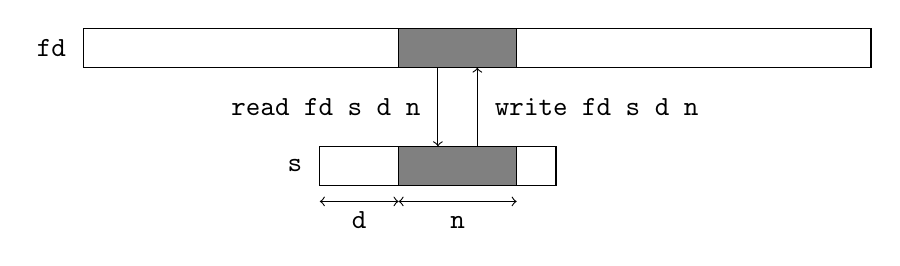
\begin{tikzpicture}[font={\ttfamily}]
\path[draw,fill=gray] (1,1.5) rectangle +(1.5, 0.5);
\path[draw] (-3,1.5) rectangle +(10, 0.5);
\node[anchor=east] at (-3.1,1.75) {fd};

\draw[->] (1.5, 1.5) to node [left=1mm] {read fd s d n} (1.5, 0.5);
\draw[<-] (2, 1.5) to node [right=1mm] {write fd s d n} (2, 0.5);

\path[draw,fill=gray] (1,0) rectangle +(1.5, 0.5);
\path[draw] (0,0) rectangle (3, 0.5);
\node[anchor=east] at (-0.1,0.25) {s};

\draw[<->] (0,-0.2) to node [below] {\phantom{n}d\phantom{n}} (1,-0.2);
\draw[<->] (1,-0.2) to node [below] {\phantom{d}n\phantom{d}} (2.5,-0.2);
\end{tikzpicture}
\end{myimage}
%
% \ml+read+ and \ml+single_write+ return the number of bytes actually
% read or written.
\ml+read+ と \ml+single_write+ は実際に読み込んだ/書き込んだバイト数を返します。

% Reads and write calls are performed from the file descriptor's current
% read/write position (if the file was opened in \ml+O_APPEND+ mode,
% this position is set at the end of the file prior to any
% write). After the system call, the current position is advanced by
% the number of bytes read or written.
入出力の命令はファイルディスクリプタの現在の入出力位置から行われます (ファイルが \ml+O_APPEND+ モードで開かれた場合、この位置は書き込み命令の前にファイルの末尾にセットされます)。システムコールの後、現在位置は読み込み/書き込みを行ったバイト数だけ進みます。


% For writes, the number of bytes actually written is usually the number
% of bytes requested. However there are exceptions: (i) if it is not
% possible to write the bytes (\eg{} if the disk is full) (ii) the
% descriptor is a pipe or a socket open in non-blocking mode (iii) due to
% {\ocaml}, if the write is too large.
書き込みでは実際に書き込むバイト数は要求されたバイト数と普通一致しますが、いくつか例外があります:
(i) バイト列を書き込めなかった場合 (例えばディスクが満杯なとき)
(ii) ディスクリプタがノンブロッキングモードで開かれたパイプまたはソケットな場合
(iii) 書き込む文字列が \ocaml の持つバッファより大きい場合

% The reason for (iii) is that internally {\ocaml} uses auxiliary
% buffers whose size is bounded by a maximal value. If this value is
% exceeded the write will be partial. To work around this problem
% {\ocaml} also provides the function \libvalue{Unix}{write} which
% iterates the writes until all the data is written or an error occurs.
% The problem is that in case of error there's no way to know the number
% of bytes that were actually written. Hence \ml+single_write+ should be
% preferred because it preserves the atomicity of writes (we know
% exactly what was written) and it is more faithful to the original Unix
% system call (note that the implementation of \ml+single_write+ is
% described in section~\ref{single_write}).
(iii) の理由は \ocaml が最大値の制限された補助バッファを使っているためです。バッファの最大値よりも書き込みが大きかった場合、書き込みは部分的になります。この問題を解決するために、 \ocaml には エラーが出るか全てのデータが書き込まれるまで書き込みを繰り返す \libvalue{Unix}{write} があります。しかしこの関数を使うとエラーが起こった場合に書き込まれたバイト数を知ることができません。\ml+single_write+を使うと書き込みの原始的になり(何が書き込まれたかが分かる)、オリジナルの Unix システムコールにより忠実になるので \ml+single_write+ を使うべきです。\ml+single_write+ の実装はセクション~\ref{single_write} で説明されています。

%%% The french version has that here, but I don't think it belongs
%%% here.
%% In the following chapter, we shall see that when we write to a
%% file descriptor which refers to a pipe or a lock file placed
%% in input/output blocking mode and which is then interrupted by a signal,
%% the call \ml+single_write+ returns an error \ml+EINTR+.

\begin{example}
% Assume \ml+fd+ is a descriptor open in write-only mode.
\ml+fd+ が書き込み専用モードで開かれたディスクリプタだとします。
%
\begin{lstlisting}
write fd "Hello world!" 3 7
\end{lstlisting}
%
% writes the characters \ml+"lo worl"+ in the corresponding file,
% and returns 7.
は \ml+"lo worl"+ という文字列を対応するファイルに書き込み、 7 を返します。
\end{example}

% For reads, it is possible that the number bytes actually read is
% smaller than the number of requested bytes. For example when the end
% of file is near, that is when the number of bytes between the current
% position and the end of file is less than the number of requested
% bytes. In particular, when the current position is at the end of file,
% \ml+read+ returns zero. The convention \quotes{zero equals end of
%   file} also holds for special files, pipes and sockets. For example,
% \ml+read+ on a terminal returns zero if we issue a \ml+ctrl-D+ on the
% input.
読み込みでは実際に読み込んだバイト数が読むように要求されたバイト数よりも小さいことがありえます。例えばファイルの終端が近いときは現在位置からファイルの終端までのバイト数が要求されたバイト数よりも小さくなります。特に現在位置がファイルの終端なとき \ml+read+ は 0 を返します。\quotes{ゼロはファイルの終端と等しい} という慣習はスペシャルファイルやパイプ、ソケットに対しても成り立ちます。例えば \ml+ctrl-D+ を端末に入力すると \ml+read+ は 0 を返します。

% Another example is when we read from a terminal. In that case,
% \ml+read+ blocks until an entire line is available. If the line length
% is smaller than the requested bytes \ml+read+ returns immediately with
% the line without waiting for more data to reach the number of
% requested bytes. (This is the default behavior for terminals, but it
% can be changed to read character-by-character instead of
% line-by-line, see section~\ref{sec/speciaux} and the type
% \libtype{Unix}{terminal\_io} for more details.)
\ml+read+ が要求した値よりも小さい値を返すもうひとつの例は端末から読み込む場合です。この場合 \ml+read+ はまず行の入力が利用可能になるまでブロックします。行が入力され、その長さが要求されたバイト数よりも短い場合、\ml+read+ は要求されたバイト数に達しようと次のデータを待つことをせずに行の入力が利用可能になった時点で値を返します(これは端末のデフォルトの動作ですが、文字ごとに読み込むように変えることもできます。セクション section~\ref{sec/speciaux} と \libtype{Unix}{terminal\_io} 型を参考にしてください)。

\begin{example}
% The following expression reads at most 100 characters from standard
% input and returns them as a string.
次のプログラムは標準入力から最大 100 文字を読み込み、文字列として返します。
%
\begin{lstlisting}
let buffer = Bytes.create 100 in
let n = read stdin buffer 0 100 in
  Bytes.sub buffer 0 n
\end{lstlisting}
\end{example}

\begin{example}
% The function \ml+really_read+ below has the same interface as
% \ml+read+, but makes additional read attempts to try to get
% the number of requested bytes. It raises the exception
% \ml+End_of_file+ if the end of file is reached while doing this.
以下の関数 \ml+really_read+ は \ml+read+ と同じインターフェースを持ちますが、要求されたバイト数を取得するために追加の読み込みを行います。読み込み中にファイルの終端に達した場合には \ml+End_of_file+ 例外が出ます。
%
\begin{lstlisting}
let rec really_read fd buffer start length =
  if length <= 0 then () else
  match read fd buffer start length with
  | 0 -> raise End_of_file
  | r -> really_read fd buffer (start + r) (length - r);;
\end{lstlisting}
%
\end{example}

\section{ディスクリプタのクローズ}

% The system call \syscall{close} closes a file descriptor.
システムコール \syscall{close} はファイルディスクリプタを閉じます。
%
\begin{listingcodefile}{tmpunix.mli}
val $\libvalue{Unix}{close}$ : file_descr -> unit
\end{listingcodefile}
%

% Once a descriptor is closed, all attempts to read, write, or do
% anything else with the descriptor will fail. Descriptors should be
% closed when they are no longer needed; but it is not mandatory. In
% particular, and in contrast to \ml+Pervasives+'
% channels, a file descriptor doesn't need to be closed to ensure that
% all pending writes have been performed as write requests made with
% \ml+write+ are immediately transmitted to the kernel. On the other
% hand, the number of descriptors allocated by a process is limited by
% the kernel (from several hundreds to thousands). Doing a \ml+close+ on
% an unused descriptor releases it, so that the process does not run out
% of descriptors.
ディスクリプタが閉じられると読み込みや書き込みなどのディスクリプタに関する操作は全て失敗します。ディスクリプタは必要なくなった時点で閉じられるべきですが、閉じることは必須ではありません。\ml+write+ 関数による書き込みの要求が即時にカーネルに伝わるために、\ml+Pervasives+ モジュールのチャンネルとは違って全ての書き込みが実行されたことを保証するためにチャンネルを閉じる必要はありません。一方プロセスが確保できるディスクリプタの数はカーネルによって (数百から数千に) 制限されていることから、使わないディスクリプタを \ml+close+ で開放しないとディスクリプタが枯渇します。

% \section{\label{ex/filecopy}Complete example: file copy}
\section{\label{ex/filecopy}完全な例: ファイルのコピー}

% We program a command \ml+file_copy+ which, given two arguments
% \ml+f1+ and \ml+f2+, copies to the file \ml+f2+ the bytes contained
% in \ml+f1+.
引数として与えられる \ml+f1+ と \ml+f2+ について、\ml+f1+ のバイト列を \ml+f2+ にコピーするコマンド \ml+file_copy+ を作ります。
%
\begin{listingcodefile}{file_copy.ml}
open Unix;;

let buffer_size = 8192;;
let buffer = Bytes.create buffer_size;;

let file_copy input_name output_name =
  let fd_in = openfile input_name [O_RDONLY] 0 in
  let fd_out = openfile output_name [O_WRONLY; O_CREAT; O_TRUNC] 0o666 in
  let rec copy_loop () = match read fd_in buffer 0 buffer_size with
    |  0 -> ()
    | r -> ignore (write fd_out buffer 0 r); copy_loop ()
  in
  copy_loop ();
  close fd_in;
  close fd_out;;
\end{listingcodefile}
%
\begin{codefile}{copy.ml}
open Unix
open File_copy
\end{codefile}
%
\begin{listingcodefile}{copy.ml}
let copy () =
  if Array.length Sys.argv = 3 then begin
    file_copy Sys.argv.(1) Sys.argv.(2);
    exit 0
  end else begin
    prerr_endline
      ("Usage: " ^ Sys.argv.(0) ^ " <input_file> <output_file>");
    exit 1
  end;;

handle_unix_error copy ();;
\end{listingcodefile}
%

% The bulk of the work is performed by the the function \ml+file_copy+.
% First we open a descriptor in read-only mode on the input file and
% another in write-only mode on the output file.
作業の多くは \ml+file_copy+ 関数によって実行されます。最初に入力ファイルのディスクリプタを読み込み専用で開き、次に出力ファイルのディスクリプタを書き込み専用モードで開きます。

% If the output file already exists, it is truncated (option
% \ml+O_TRUNC+) and if it does not exist it is created (option
% \ml+O_CREAT+) with the permissions \ml+rw-rw-rw-+ modified by the creation
% mask. (This is unsatisfactory: if we copy an executable file, we would
% like the copy to be also executable. We will see later how to give
% a copy the same permissions as the original.)
出力ファイルがすでに存在している場合ファイルは切り捨てられ (\ml+O_TRUNC+ オプション)、存在しない場合には作成されます (\ml+O_CREAT+ オプション)。作成されるファイルの権限は \ml+rw-rw-rw-+ をファイル作成マスクで改変したものですが、これは十分ではありません。実行可能ファイルをコピーする場合は、コピー先も実行可能であるべきだからです。コピー先のファイルと元のファイルの権限を同じにする方法は後述します。

% In the \ml+copy_loop+ function we do the copy by blocks of
% \ml+buffer_size+ bytes. We request \ml+buffer_size+ bytes to read. If
% \ml+read+ returns zero, we have reached the end of file and the copy
% is over. Otherwise we write the \ml+r+ bytes we have read in the
% output file and start again.
\ml+copy_loop+ 関数の中で \ml+buffer_size+ バイトのコピーを行います。まず\ml+buffer_size+ の読み込みを行い、これが 0 を返した場合はファイルの終端に到達しているのでコピーを終了します。そうでなければ読み込んだ \ml+r+ バイトを出力ファイルに書き込んで同じことを繰り返します。

% Finally, we close the two descriptors. The main program \ml+copy+
% verifies that the command received two arguments and passes them to
% the function \ml+file_copy+.
最後に二つのディスクリプタを閉めます。プログラム本体となる \ml+copy+ はコマンドが二つの引数を受け取ったことを確認し、その引数を \ml+file_copy+ 関数に渡します。

% Any error occurring during the copy results in a \ml+Unix_error+
% caught and displayed by \ml+handle_unix_error+. Example of errors
% include inability to open the input file because it does not
% exist, failure to read because of restricted permissions, failure to
% write because the disk is full, \etc
コピー中に起きた \ml+Unix_error+ は\ml+handle_unix_error+ によって補足され、エラーの内容が表示されます。ここで起こるエラーの例としては入力ファイルが存在しないために開くことができない、権限が足りなくてファイルを開くことができない、ディスクに容量がなくて書き込むことができない、などがあります。


\begin{exercise}
% Add an option \ml+-a+ to the program, such that
% \ml+file_copy -a f1 f2+ appends the contents of \ml+f1+ to the end of
% the file \ml+f2+.
\ml+file_copy -a f1 f2+ が \ml+f1+ の内容を \ml+f2+ の末尾に付け足すように、\ml+-a+ オプションを追加してください。
\end{exercise}
\begin{answer}
% If the option \ml+-a+ is supplied, we need to do
\ml+-a+ オプションが与えられた場合、行うべき処理が
%
\begin{lstlisting}
openfile output_name [O_WRONLY; O_CREAT; O_APPEND] 0o666
\end{lstlisting}
%
% instead of
ではなく
%
\begin{lstlisting}
openfile output_name [O_WRONLY; O_CREAT; O_TRUNC] 0o666
\end{lstlisting}
%
% Parsing the new option from the command line is left to the reader.
となります。 新しいオプションをコマンドラインからパースする部分は読者に残します。
\end{answer}

% \section{The cost of system calls and buffers}
\section{システムコールのコストとバッファ}

% In the example \ml+file_copy+, reads were made in blocks of 8192
% bytes. Why not read byte per by byte, or megabyte per by megabyte?
% The reason is efficiency.
\ml+file_copy+ の例では読み込みを 8192 バイトごとに行ないました。どうして 1 バイトごとや 1 メガバイトごとに読み込みをしないのでしょうか? 理由は効率です。
% Figure~\ref{fig/copy-speed} shows the copy speed of \ml+file_copy+, in
% bytes per second, against the size of blocks (the value
% \ml+buffer_size+). The amount of data transferred is the same
% regardless of the size of the blocks.
図~\ref{fig/copy-speed} に \ml+file_copy+ の速度を示します。一秒間にコピーできるバイト数を縦軸に、ブロックサイズ (\ml+buffer_size+ の値) を横軸に示しています。
\begin{myfigure}
\begin{myimage}[width="100\%"]
\begin{tikzpicture}[font=\tiny]
\pgfsetplotmarksize{0.8pt}
\draw plot[only marks,mark=*] file {data/speed-log.data};

% x-axis
\draw (0,-1) -- (7,-1);
\foreach \x in {0,...,7} { \draw (\x,-1) -- (\x,-0.95); };
\node at (0,-1.3) {\phantom{$^{2}$}1\phantom{$^{2}$}};
\node at (1,-1.3) {\phantom{$^{2}$}10\phantom{$^{2}$}};
\node at (2,-1.3) {\phantom{$^{2}$}100\phantom{$^{2}$}};
\foreach \x in {3,...,7} { \node at (\x,-1.3) {\phantom{$^{\x}$}10$^\x$}; };
\node at (8.5, -1.3) {Size (bytes)\phantom{1$^{1}$}};

% y-axis
\draw (-0.5,-0.5) -- (-0.5, 2.5);
\foreach \y in {-1,...,3} { \draw (-0.5,\y) -- (-0.45,\y); };
\node[anchor=east] at (-0.5,-1) {0.1\phantom{$^{3}$}};
\node[anchor=east] at (-0.5,0) {1\phantom{$^{3}$}};
\node[anchor=east] at (-0.5,1) {10\phantom{$^{3}$}};
\node[anchor=east] at (-0.5,2) {100\phantom{$^{3}$}};
\node[anchor=east] at (-0.5,3) {10$^{3}$};

\node[anchor=east] at (-0.5,3.5) {Speed (MB/s)};
\end{tikzpicture}
\end{myimage}
% \caption{Copy speed as a function of block size}
\caption{ブロックサイズの関数としてのコピー速度}
\label{fig/copy-speed}
\end{myfigure}
% For small block sizes, the copy speed is almost proportional to the
% block size. Most of the time is spent not in data transfers but in the
% execution of the loop \ml+copy_loop+ and in the calls to \ml+read+ and
% \ml+write+. By profiling more carefully we can see that most of the
% time is spent in the calls to \ml+read+ and \ml+write+. We conclude
% that a system call, even if it has not much to do, takes a minimum of
% about 4 micro-seconds (on the machine that was used for the test~---~a
% 2.8 GHz Pentium 4 ), let us say from 1 to 10 microseconds.  For small
% input/output blocks, the duration of the system call dominates.
転送されるデータの総量はブロックサイズに関わらず一定です。ブロックサイズが小さい時は、コピー速度はブロックサイズにほぼ比例しています。実行時間の多くがはデータの転送ではなく、\ml+copy_loop+ のループと \ml+read+ と \ml+write+ の呼び出しに使われているということがわかります。更に詳細に実行時間を計測すると、ほとんどが \ml+read+ と \ml+write+ の呼び出しに使われていることがわかります。システムコールは処理が大きくない場合でも (テストに使われた PC~---~2.8 GHz Pentium 4~---~ では) 最低 4 マイクロ秒、一般的には 1 から 10 マイクロ秒程度かかります。そのため入出力のブロックサイズが小さい場合にはシステムコールの時間が支配的になります。

% For larger blocks, between 4KB and 1MB, the copy speed is constant and
% maximal. Here, the time spent in system calls and the loop is small
% relative to the time spent on the data transfer. Also, the buffer
% size becomes bigger than the cache sizes used by the system and the
% time spent by the system to make the transfer dominates the cost of a
% system call\footnote{In fact, {\ocaml} limits the size of data
%   transfers to 16KB (in the current version) and repeats \ml+write+
%   system calls to make the complete transfer~---~see the discussion in
%   section~\ref{single_write}. But this limit is bigger than the
%   size of system caches and it is not observable.}.
ブロックが大きくて 4KB から 1MB の場合、コピー速度は最大値で一定です。ここではシステムコールとループにかかる時間がデータ転送にかかる時間に比べて小さくなっているということです。加えてバッファのサイズがシステムのキャッシュよりも大きくなるためにデータの転送がシステムコールのコストを上回るようになります\footnote{実際には \ocaml はデータ転送を (現在のバージョンでは) 16KB に制限し全体の転送が終わるまで \ml+write+ システムコールを繰り返します~---~セクション~\ref{single_write} 参照。しかしこの制限はシステムのキャッシュサイズよりも大きいので無視できます。}。

% Finally, for very large blocks (8MB and more) the speed is slightly
% under the maximum.  Coming into play here is the time needed to
% allocate the block and assign memory pages to it as it fills up.
最後に、ブロックがとても大きい (8 MB 以上) ときにはコピー速度は最大値よりも少しだけ小さくなります。ここで影響するのはブロックを確保してメモリのページを割り当てるのを書き込み中に行う時間です。

\begin{codefile}{speed_write.c}
#include <errno.h>
#include <string.h>
#include <caml/mlvalues.h>
#include <caml/memory.h>
#include <caml/signals.h>
#include <caml/unixsupport.h>

#define LONG_BUFFER_SIZE 9388608

CAMLprim value speed_write
        (value fd, value buf, value ofs, value len) {
  CAMLparam4(fd, buf, ofs, len);
  long numbytes;
  int ret = 0;
  char iobuf[LONG_BUFFER_SIZE];
  numbytes = Long_val(len);
  if (numbytes > LONG_BUFFER_SIZE) numbytes = LONG_BUFFER_SIZE;
  /* memmove (iobuf, &Byte(buf, Long_val(ofs)), numbytes); */
  /* enter_blocking_section (); */
  /* ret = write(Int_val(fd), iobuf, (int) numbytes); */
  ret = write(Int_val(fd), &Byte(buf, Long_val(ofs)), (int) numbytes);
  /* leave_blocking_section (); */
  if (ret == -1) uerror("write", Nothing);
  CAMLreturn (Val_int(ret));
}
\end{codefile}
%
\begin{codefile}{speed.ed}
f speed.ml
r file_copy.ml
3a
external speed_write :
   file_descr -> string -> int -> int -> int = "speed_write";;
.
/buffer_size/,/file_copy/c
let file_copy buffer_size input_name output_name =
  let buffer = Bytes.create buffer_size in
.
/write/s/write/speed_write/
$a

let rec power n k = if k > 0 then n * power n (pred k) else 1;;
let copy () =
  if Array.length Sys.argv = 2 then begin
    let file = Sys.argv.(1) in
    let tmp = Filename.temp_file "foo" "bar" in
    let mega_octets = float (10 * (lstat file).st_size) /. 1e6 in
    (* put file in cache *)
    file_copy 10 file "/dev/null";
    for i = 23 downto 0 do
      let start = let t = Unix.times () in t.tms_utime +. t.tms_stime in
      let block = power 2 i in
      for i = 1 to 10 do file_copy block file tmp done;
      let stop = let t = Unix.times () in t.tms_utime +. t.tms_stime in
      let time = stop -. start in
      let speed = mega_octets /. time in
      Printf.printf "%9d %.2f" block speed;
      print_newline ();
    done;
      exit 0
  end else begin
    prerr_endline ("Usage: " ^Sys.argv.(0)^ " <input_file> <output_file>");
    exit 1
  end;;

handle_unix_error copy ();;
.
wq
\end{codefile}
% $

% The moral of the story is that, a system call, even if it does very little work,
% costs dearly~---~much more than a normal function call: roughly, 2 to
% 20 microseconds for each system call, depending on the
% architecture. It is therefore important to minimize the number of
% system calls. In particular, read and write operations should be made
% in blocks of reasonable size and not character by character.
以上のことから学べることは、システムコールはほとんど何も処理をしていない場合でも大きな~---~通常の関数呼び出しよりもはるかに大きな~---~コストがかかるということです。アーキテクチャによって違いますが、だいたい 2 から 20 マイクロ秒が呼び出しごとにかかります。そのためシステムコールの数を減らすことが重要になります。読み込みと書き込みに関して言えば、一文字ごとではなくある程度のサイズのブロックごとに行われるべきです。

% In examples like \ml+file_copy+, it is not difficult to do
% input/output with large blocks. But other types of programs are more
% naturally written with character by character input or output (\eg{}
% reading a line from a file, lexical analysis, displaying a number \etc).
% To satisfy the needs of these programs, most systems provide
% input/output libraries with an additional layer of software between
% the application and the operating system. For example, in {\ocaml} the
% \ml+Pervasives+ module defines the abstract types
% \libtype{Pervasives}{in\_channel} and
% \libtype{Pervasives}{out\_channel}, similar to file descriptors, and
% functions on these types like \libvalue{Pervasives}{input\_char},
% \libvalue{Pervasives}{input\_line},
% \libvalue{Pervasives}{output\_char}, or
% \libvalue{Pervasives}{output\_string}.  This layer uses buffers to
% group sequences of character by character reads or writes into a
% single system call to read or write. This results in better
% performance for programs that proceed character by character.
% Moreover this additional layer makes programs more portable: we just
% need to implement this layer with the system calls provided by another
% operating system to port all the programs that use this library on
% this new platform.
\ml+file_copy+ の例では大きなブロックで入出力を行うのは難しくありません。しかしある種のプログラムでは一文字ごとに入出力を行うことが自然なことがあります(例えばファイルから一行ずつ読む処理、字句解析、数字の印字など)。このようなプログラムのために、ほとんどのシステムにはアプリケーションとオペレーティングシステムの間にソフトウェアのレイヤーを追加する入出力ライブラリがあります。例えば \ocaml には \ml+Pervasives+ モジュールにファイルディスクリプタと似た抽象型\libtype{Pervasives}{in\_channel} と \libtype{Pervasives}{out\_channel} が定義されていて、この型に関する関数 \libvalue{Pervasives}{input\_char},\libvalue{Pervasives}{input\_line}、\libvalue{Pervasives}{output\_char} あるいは \libvalue{Pervasives}{output\_string} があります。このレイヤーはバッファを使って複数回の一文字ごとの読み込みと書き込みを一回のシステムコールにまとめます。これによって一文字ごとに処理をするプログラムの効率が良くなります。さらにこのレイヤーによってプログラムがよりポータブルになります。\ml+Pervasives+ モジュールを使うプログラムを新しいオペレーティングシステムに移植するには、このライブラリをそのシステム上で使えるシステムコールを使って実装すれば良いからです。


% \section{Complete example: a small input/output library}
\section{完全な例: 簡単な入出力ライブラリ}

% To illustrate the buffered input/output techniques, we implement a fragment
% of {\ocaml} \ml+Pervasives+ library. Here is the interface:
バッファを使った入出力のテクニックの例として、\ocaml の \ml+Pervasives+ ライブラリの一部を実装します。 次のようなインタフェースを持ちます:
%
\begin{listingcodefile}{io.mli}
exception End_of_file

type in_channel
val open_in : string -> in_channel
val input_char : in_channel -> char
val close_in : in_channel -> unit

type out_channel
val open_out : string -> out_channel
val output_char : out_channel -> char -> unit
val close_out : out_channel -> unit
\end{listingcodefile}
%
% We start with the \quotes{input} part. The abstract type
% \ml+in_channel+ is defined as follows:
\quotes{読み込み} の部分から始めます。
抽象型 \ml+in_channel+ は次のように定義します:
%
\begin{listingcodefile}{io.ml}
open Unix;;

type in_channel =
  { in_buffer: bytes;
    in_fd: file_descr;
    mutable in_pos: int;
    mutable in_end: int };;
exception End_of_file
\end{listingcodefile}
%
% The character string of the \ml+in_buffer+ field is, literally, the
% buffer.  The field \ml+in_fd+ is a (Unix) file descriptor, opened on
% the file to read. The field \ml+in_pos+ is the current read position
% in the buffer.  The field \ml+in_end+ is the number of valid
% characters preloaded in the buffer.
文字列 \ml+in_buffer+ は文字通りのバッファです。フィールド \ml+in_fd+ は読み込むファイルに開かれた (Unix の) ファイルディスクリプタです。フィールド \ml+in_pos+ は読み込みの現在位置を示します。フィールド \ml+in_end+ は事前にバッファへ読み込まれた文字列のうち有効な部分長さです。
%
\begin{myimage}[width="85\%"]
\begin{tikzpicture}
\path[draw] (-3,2.5) rectangle +(10, 0.5);
\node[anchor=east] at (-3.1,2.75) {\texttt{in\_fd}};
\draw[dashed] (1,3) to node [left=2mm,text width=2.0cm,text centered]
% {characters read} (1,0);
{読み込んだ\\文字列} (1,0);

\draw[dashed] (4,3) to node [left=1mm,text width=2.5cm,text centered]
% {buffered characters to read} (4,0);
{バッファされ\\これから読み\\込まれる文字列} (4,0);

\path[draw] (-1,0) rectangle +(6, 0.5);
\node[anchor=east] at (-1.1,0.25) {\texttt{in\_buffer}};

% \node (fdpos) at (4,3.75) {read position of \texttt{in\_fd}};
\node (fdpos) at (4,3.75) {読み込み位置 \texttt{in\_fd}};
\draw[->] (fdpos.south) to (4,3);

\node (ipos) at (1,-0.75) {\texttt{\phantom{d}in\_pos\phantom{d}}};
\node (iend) at (4,-0.75) {\texttt{\phantom{p}in\_end\phantom{p}}};
\draw[->] (ipos.north) to (1,0);
\draw[->] (iend.north) to (4,0);
\end{tikzpicture}
\end{myimage}
% The fields \ml+in_pos+ and \ml+in_end+ will be modified in place during
% read operations; we therefore declare them as \ml+mutable+.
\ml+in_pos+ と \ml+in_end+ のフィールドは読み込み処理中に更新されるので \ml+mutable+ として宣言します。
%
\begin{listingcodefile}{io.ml}
let buffer_size = 8192;;
let open_in filename =
  { in_buffer = Bytes.create buffer_size;
    in_fd = openfile filename [O_RDONLY] 0;
    in_pos = 0;
    in_end = 0 };;
\end{listingcodefile}
%
% When we open a file for reading, we create a buffer of reasonable size
% (large enough so as not to make too many system calls; small enough so
% as not to waste memory). We then initialize the field \ml+in_fd+ with
% a Unix file descriptor opened in read-only mode on the given file. The
% buffer is initially empty (it does not contain any character from the
% file); the field \ml+in_end+ is therefore initialized to zero.
読み込みのためにファイルを開いたとき、同時に合理的なサイズの (システムコールが多くなりすぎない程度に大きく、メモリを無駄遣いしない程度に小さい) バッファを作ります。その後 \ml+in_fd+ フィールドを読み込み専用で開いたファイルに対する Unix のファイルディスクリプタで初期化します。バッファは最初空です (ファイルからのどんな文字列も含んでいません) 。そのため \ml+in_end+ フィールドは 0 で初期化します。
%
\begin{listingcodefile}{io.ml}
let input_char chan =
  if chan.in_pos < chan.in_end then begin
    let c =  chan.in_buffer.[chan.in_pos] in
      chan.in_pos <- chan.in_pos + 1;
      c
  end else begin
    match read chan.in_fd chan.in_buffer 0 buffer_size
    with 0 -> raise End_of_file
       | r -> chan.in_end <- r;
              chan.in_pos <- 1;
              chan.in_buffer.[0]
  end;;
\end{listingcodefile}
%
% To read a character from an \ml+in_channel+, we do one of two
% things.  Either there is at least one unread character in the buffer;
% that is to say, the field \ml+in_pos+ is less than the field
% \ml+in_end+. We then return this character located at \ml+in_pos+, and
% increment \ml+in_pos+. Or the buffer is empty and we call \ml+read+ to
% refill the buffer. If \ml+read+ returns zero, we have reached the end
% of the file and we raise the exception \ml+End_of_file+. Otherwise, we
% put the number of characters read in the field \ml+in_end+ (we may
% receive less characters than we requested, thus the buffer may be
% only partially refilled) and we return the first character read.
\ml+in_channel+ から文字を読むとき、次の二つのうち一つを行います。一つ目はバッファに一つ以上まだ読んでいない文字がある、つまり \ml+in_pos+ フィールドの値が \ml+in_end+ フィールドの値よりも小さい場合です。このときはバッファの \ml+in_pos+ にある文字を返し、 \ml+in_pos+ をインクリメントします。もう一つはバッファが空の場合で、このときは \ml+read+ を呼んでバッファにもう一度文字列を読み込みます。\ml+read+ が 0 を返したならファイルの終端に達したということなので \ml+End_of_file+ 例外を出します。そうでなければ \ml+in_end+ に呼んだ文字の数を代入します。
%
\begin{listingcodefile}{io.ml}
let close_in chan =
  close chan.in_fd;;
\end{listingcodefile}
%
% Closing an \ml+in_channel+ just closes the underlying Unix file descriptor.
\ml+in_channel+ を閉じる処理は対応する Unix のファイルディスクリプタを閉じるだけです。

% The \quotes{output} part is very similar to the \quotes{input}
% part. The only asymmetry is that the buffer now contains incomplete
% writes (characters that have already been buffered but not written to
% the file descriptor), and not reads in advance (characters that have
% buffered, but not yet read).
\quotes{書き込み} の部分は \quotes{読み込み} の部分にとても良く似ています。唯一異なるのはバッファがまだ読んでいない読み込み (バッファされたが読み込まれていない文字列) を保持するのではなくて、まだ完了していない書き込み (バッファされたがファイルディスクリプタに書き込まれていない文字列) を保持する点です。

\begin{myimage}[width="85\%"]
\begin{tikzpicture}
\path[draw] (-3,2.5) rectangle +(10, 0.5);
\node[anchor=east] at (-3.1,2.75) {\texttt{out\_fd}};
\draw[dashed] (1,3) to node [left=2mm,text width=2cm,text centered]
% {written characters} (1,0);
{書き込んだ\\文字列} (1,0);

\draw[dashed] (4,3) to node [left,text width=2.5cm,text centered]
% {buffered characters to write} (4,0);
{バッファされ\\これから書き\\込まれる文字列} (4,0);

\path[draw] (1,0) rectangle +(4, 0.5);
\node[anchor=east] at (0.9,0.25) {\texttt{out\_buffer}};

% \node (fdpos) at (1,3.75) {write position of \texttt{out\_fd}};
\node (fdpos) at (1,3.75) {書き込み位置 \texttt{out\_fd}};
\draw[->] (fdpos.south) to (1,3);

\node (opos) at (4,-0.75) {\texttt{out\_pos}};
\draw[->] (opos.north) to (4,0);
\end{tikzpicture}
\end{myimage}
%
\begin{listingcodefile}{io.ml}
type out_channel =
  { out_buffer: bytes;
    out_fd: file_descr;
    mutable out_pos: int };;

let open_out filename =
  { out_buffer = Bytes.create 8192;
    out_fd = openfile filename [O_WRONLY; O_TRUNC; O_CREAT] 0o666;
    out_pos = 0 };;

let output_char chan c =
  if chan.out_pos < Bytes.length chan.out_buffer then begin
    chan.out_buffer.[chan.out_pos] <- c;
    chan.out_pos <- chan.out_pos + 1
  end else begin
    ignore (write chan.out_fd chan.out_buffer 0 chan.out_pos);
    chan.out_buffer.[0] <- c;
    chan.out_pos <- 1
  end;;

let close_out chan =
  ignore (write chan.out_fd chan.out_buffer 0 chan.out_pos);
  close chan.out_fd;;
\end{listingcodefile}
%
% To write a character on an \ml+out_channel+, we do one of two things.
% Either the buffer is not full and we just store the character in the
% buffer at the position \ml+out_pos+ and increment that value. Or the
% buffer is full and we empty it with a call to \ml+write+ and then
% store the character at the beginning of the buffer.
\ml+out_channel+ に文字を書き込むには次の二つのうち一つを行います。一つ目はバッファが満杯ではない場合で、このときは文字をバッファを \ml+out_pos+ の位置に保存して \ml+out_pos+ をインクリメントします。もう一つはバッファが満杯の場合で、このときは \ml+write+ を呼んでバッファを空にしてからバッファの先頭に文字を読み込みます。

% When we close an \ml+out_channel+, we must not forget to write the
% buffer contents (the characters from 0 to \ml+out_pos - 1+) to the
% file otherwise the writes made on the channel since the last time
% the buffer was emptied would be lost.
\ml+out_channel+ を閉めるときにはバッファの内容 (位置 0 から \ml+out_pos - 1+ までの文字列) を書き込むことを忘れないでください。これを忘れると最後にバッファが空になってからチャンネルに書き込まれた内容が失われます。

\begin{exercise}
% Implement the function:
次の関数を実装してください:
%
\begin{lstlisting}
val output_string : out_channel -> string -> unit
\end{lstlisting}
%
% which behaves like a sequence of \ml+output_char+ on each
% character of the string, but is more efficient.
この関数は \ml+output_char+ をそれぞれの文字に対して複数回呼んだときと同じ動作をしますが、より効率的です。
\enlargethispage{2\baselineskip} %% To avoid a widow
\end{exercise}
\begin{answer}
% The idea is to copy the string to output into the buffer. We need to
% take into account the case where there is not enough space in the
% buffer (in that case the buffer needs to emptied), and also the case
% where the string is longer than the buffer (in that case it can
% be written directly). Here is a possible solution.
書き込む文字列をバッファにコピーするのが基本的なアイデアです。バッファに十分な空きが無く途中でバッファを空にする必要がある場合とそうでなく文字列全てをバッファに直接書き込める場合とを考える必要があります。解答例を以下に示します。
%
\begin{lstlisting}
open Unix;;
\end{lstlisting}
%
\begin{lstlisting}
let output_string chan s =
  let avail = Bytes.length chan.out_buffer - chan.out_pos in
  if Bytes.length s <= avail then begin
    Bytes.blit s 0 chan.out_buffer chan.out_pos (Bytes.length s);
    chan.out_pos <- chan.out_pos + Bytes.length s
  end
  else if chan.out_pos = 0 then begin
    ignore (write chan.out_fd s 0 (Bytes.length s))
  end
  else begin
    Bytes.blit s 0 chan.out_buffer chan.out_pos avail;
    let out_buffer_size = Bytes.length chan.out_buffer in
    ignore (write chan.out_fd chan.out_buffer 0 out_buffer_size);
    let remaining = Bytes.length s - avail in
    if remaining < out_buffer_size then begin
      Bytes.blit s avail chan.out_buffer 0 remaining;
      chan.out_pos <- remaining
    end else begin
      ignore (write chan.out_fd s avail remaining);
      chan.out_pos <- 0
    end
  end;;
\end{lstlisting}
%
\begin{lstlisting}
let ex2 () =
  if Array.length Sys.argv < 3 then begin
     prerr_string "Usage: test <sources> <dest>";
     exit 2;
  end;
  let fdin = open_in Sys.argv.(1) in
  let fdout = open_out Sys.argv.(2) in
  prerr_endline "copying";
  try while true do output_char fdout (input_char fdin) done
  with End_of_file ->
   prerr_endline "Done";
   output_string fdout "The end.\n";
   prerr_endline "Closing";
   close_out fdout;;

handle_unix_error ex2 ();;
\end{lstlisting}
%
\begin{lstlisting}
./ex2.byte ex2.ml ex2.out
(cat ex2.ml; echo "C'est la fin.") | diff --brief - ex2.out
rm ex2.out
\end{lstlisting}
\end{answer}


% \section{Positioning}
\section{入出力の位置}

% The system call \syscall{lseek} allows to set the current read/write
% position of a file descriptor.
システムコール \syscall{seek} はファイルディスクリプタの現在の入出力位置を変更します。
%
\begin{codefile}{tmpunix.mli}
type seek_command = Unix.seek_command
\end{codefile}
%
\begin{listingcodefile}{tmpunix.mli}
val $\libvalue{Unix}{lseek}$ : file_descr -> int -> seek_command -> int
\end{listingcodefile}
%
% The first argument is the file descriptor and the second one the
% desired position. The latter is interpreted according to the value
% of the third argument of type \libtype{Unix}{seek\_command}. This
% enumerated type specifies the kind of position:
第一引数はファイルディスクリプタで第二引数は移動させる位置です。第二引数は \libtype{Unix}{seek\_command} 型の第三引数に基づいて解釈されます。この列挙型は位置の種類を指定します:
%
\begin{mltypecases}
\begin{tabular}{@{}lp{0.8\textwidth}}
% \ml+SEEK_SET+ & Absolute position. The second argument specifies
% the character number to point to. The first character of a file is at
% position zero.\\
\ml+SEEK_SET+ & 第二引数は関数を呼び出した後の入出力位置を表す。ファイルの最初の文字は位置 0 である。 \\
%
% \ml+SEEK_CUR+ & Position relative to the current position.
% The second argument is an offset relative to the
% current position. A positive value moves forward and a negative value
%                 moves backwards.\\
\ml+SEEK_CUR+ & 第二引数は現在の入出力位置からの相対的なオフセットを表す。正の値のとき前に、負の値のとき後ろに動く。 \\
%
% \ml+SEEK_END+ & Position relative to the end of file. The
% second argument is an offset relative to the end of file.
% As for \ml+SEEK_CUR+, the offset may be positive or negative.
\ml+SEEK_END+ & 第二引数はファイルの終端からの相対的なオフセットを表す。\ml+SEEK_CUR+ と同様にオフセットは正負どちらにもなれる。
\end{tabular}
\end{mltypecases}
%
% The value returned by \ml+lseek+ is the resulting absolute
% read/write position.
\ml+lseek+ の返り値は関数を実行した後の入出力位置 (絶対位置) です。

% An error is raised if a negative absolute position is
% requested. The requested position can be located after the end
% of file. In that case, a \ml+read+ returns zero (end of
% file reached) and a \ml+write+ extends the file with zeros until
% that position and then writes the supplied data.
負の絶対位置が指定された場合はエラーとなります。ファイルの終端よりも後ろの位置を指定することは可能です。このとき \ml+read+ は (ファイルの末尾に達しているので) 0 を返し、\ml+write+ はまずファイルの終端から入出力位置まで 0 を書き込んでからデータを書き込みます。

\begin{example}
% To position the cursor on the 1000th character of a file:
カーソルを 1000 番目の文字に移動させるには以下のようにします:
%
\begin{lstlisting}
lseek fd 1000 SEEK_SET
\end{lstlisting}
%
% To rewind by one character:
一文字巻き戻すには以下のようにします:
%
\begin{lstlisting}
lseek fd (-1) SEEK_CUR
\end{lstlisting}
%
% To find out the size of a file:
ファイルのサイズを求めるには以下のようにします:
%
\begin{lstlisting}
let file_size = lseek fd 0 SEEK_END in ...
\end{lstlisting}
\end{example}

% For descriptors opened in \ml+O_APPEND+ mode, the read/write position
% is automatically set at the end of the file before each write.  Thus
% a call \ml+lseek+ is useless to set the write position, it may however
% be useful to set the read position.
ファイルディスクリプタが \ml+O_APPEND+ モードで開かれている場合、入出力位置は毎回の書き込みの前にファイルの終端にセットされます。そのため書き込み位置を指定するために \ml+lseek+ を読んでも意味がありません。一方読み込みを指定することには使えます。

% The behavior of \ml+lseek+ is undefined on certain type of files for
% which absolute access is meaningless: communication devices (pipes,
% sockets) but also many special files like the terminal.
% In most Unix implementations a call to \ml+lseek+ on these files is
% simply ignored: the read/write position is set but read/write
% operations ignore it. In some implementations, \ml+lseek+ on a pipe or
% a socket triggers an error.
コミュニケーションデバイス (パイプ、ソケット) や端末を始めとする多くのスペシャルファイルなどの、入出力の絶対位置が意味を持たないタイプのファイルについては \ml+lseek+ の動作は未定義です。Unix のほとんどの実装ではこれらのファイルに対する \ml+lseek+ は無視されます (入出力位置はセットされますが、入出力処理は入出力位置を無視します)。いくつかの実装ではパイプとソケットに対する \ml+lseek+ はエラーを出します。

\begin{exercise}
% The command \ml+tail+ displays the last $n$ lines of a file.
% How can it be implemented efficiently on regular files? What can we
% do for the other kind of files? How can the option \ml+-f+ be
% implemented (cf. \ml+man tail+)?
\ml+tail+ コマンドはファイルの末尾 $n$ 行を表示します。\ml+tail+ を通常ファイルに対して効率よく実装するにはどうすればよいでしょうか ? \ml+-f+ オプションはどのすれば実装できるでしょうか (参考: \ml+man tail+) ?
\enlargethispage{3\baselineskip} %% To avoid a widow
\end{exercise}
\begin{answer}
% A naive implementation of \ml+tail+ is to read the file sequentially
% from the beginning, keeping the last $n$ lines read in a circular
% buffer. When we reach the end of file, we display the buffer.
% When the data comes from a pipe or a special file which
% does not implement \ml+lseek+, there is no better way.
\ml+tail+ のナイーブな実装は最後に呼んだ $n$ 行を巡回バッファに記録しながらファイルを最初から読み、ファイルの末尾に達したところでバッファを表示するというものです。\ml+lseek+ の実装されないパイプやスペシャルファイルからデータが来るならば、これが最善の方法になります。

% However if the data is coming from a normal file, it is better to read
% the file from the end. With \ml+lseek+, we read the last 4096
% characters. We scan them for the end of lines. If there are at least
% $n$ of them, we output and display the corresponding lines.
% Otherwise, we start again by adding the next preceding 4096
% characters, \etc
もしデータが通常ファイルから来るならば、ファイルの末尾から読み込むほうが効率が良くなります。まず \ml+lseek+ を使って最後の 4096 文字を読み込み、その中に改行がないか調べます。$n$ 個以上の改行があるなら対応する行を出力しそうでなければ次の 4096 バイトを読み、同じことをします。

% To add the option \ml+-f+, we first proceed as above and then we go
% back at the end of the file and try to \ml+read+ from there. If
% \ml+read+ returns data we display it immediately and start again. If it
% returns \ml+0+ we wait some time (\ml+sleep 1+) and try again.
\ml+-f+ オプションを追加するにはまずオプション無しの場合の動作を行い、そのあとファイルの末尾に移動してから \ml+read+ します。\ml+read+ が返ったときはその内容をすぐに画面に表示しもう一度 \ml+read+ します。もし \ml+read+ が \ml+0+ を返したならプログラムは一定時間待ってから (\ml+sleep 1+) もう一度試します。
\end{answer}

% \section{Operations specific to certain file types}
\section{ファイルの種類に特有の操作}

% In Unix, data communication is done via file descriptors representing
% either permanent files (files, peripherals) or volatile ones (pipes
% and sockets, see chapters~\ref{sec/pipes} and \ref{sec/sockets}). File
% descriptors provide a uniform and media-independent interface for data
% communication. Of course the actual implementation of the operations
% on a file descriptor depends on the underlying media.
Unix ではデータのやり取りはディスクリプタを通して行われ、ディスクリプタは永続性のファイル (通常ファイル、周辺機器) または揮発性のファイル (パイプとソケット、 ~\ref{sec/pipes} 章と \ref{sec/sockets} 章参照) を表します。ファイルディスクリプタはデータのやり取りのための統一されたメディアによらないインタフェースを提供します。もちろんファイルディスクリプタに対する操作の実際の実装は背後にあるメディアによって異なります。

% However this uniformity breaks when we need to access all the
% features provided by a given media. General operations (opening,
% writing, reading, \etc) remain uniform on most descriptors but even,
% on certain special files, these may have an ad hoc behavior defined
% by the kind of peripheral and its parameters. There are also
% operations that work only with certain kind of media.
しかしあるメディアの全ての機能を使う必要がある場合は他のファイルと同じように扱うことはできません。ファイルのオープンや読み込み、書き込みなどの一般的な操作はほとんどのディスクリプタで同じ動作をします。しかしこのような一般的な操作であっても、周辺機器とパラメータで決まるアドホックな動作をするスペシャルファイルが存在します。またあるメディアに対してだけ可能な操作もあります。

% \subsection*{Normal files}
\subsection*{通常ファイル}

% We can shorten a normal file with the system calls
% \syscall{truncate} and \syscall{ftruncate}.
システムコール \syscall{truncate} と \syscall{ftruncate} を使うと通常ファイルを短くすることができます。
%
\begin{listingcodefile}{tmpunix.mli}
val $\libvalue{Unix}{truncate}$  : string -> int -> unit
val $\libvalue{Unix}{ftruncate}$ : file_descr -> int -> unit
\end{listingcodefile}
%
% The first argument is the file to truncate and the second the desired
% size. All the data after this position is lost.
第一引数は切り捨てるファイルで第二引数は切り捨てた後のサイズです。これより後ろの位置にある全てのデータは失われます。

% \subsection*{Symbolic links}
\subsection*{シンボリックリンク}

% Most operations on files \quotes{follow} symbolic links in the sense
% that they do not apply to the link itself but to the file on which the
% link points (for example \indexvalue{openfile},
% \indexvalue{stat}, \indexvalue{truncate}, \indexvalue{opendir}, \etc).
シンボリックリンクに対するほとんどの操作はリンクを \quotes{たどり} ます。つまり、操作はリンクそのものではなくリンクが指すファイルに適用されます (例えば \indexvalue{openfile}, \indexvalue{stat}, \indexvalue{truncate}, \indexvalue{opendir} などはこのような動作をします) 。

% The two system calls \syscall{symlink} and \syscall{readlink} operate
% specifically on symbolic links:
二つのシステムコール \syscall{symlink} と \syscall{readlink} はシンボリックリンクそのものを操作します。
%
\begin{listingcodefile}{tmpunix.mli}
val $\libvalue{Unix}{symlink}$  : string -> string -> unit
val $\libvalue{Unix}{readlink}$ : string -> string
\end{listingcodefile}
%
% The call \ml+symlink f1 f2+ creates the file \ml+f2+ as a symbolic
% link to \ml+f1+ (like the Unix command \ml+ln -s f1 f2+). The call
% \ml+readlink+ returns the content of a symbolic link, \ie{} the name of
% the file to which the link points.
\ml+symlink f1 f2+ は \ml+f1+ へのシンボリックリンク \ml+f2+ を作成します (Unix コマンド \ml+ln -s f1 f2+ と同様です) 。\ml+readlink+ はシンボリックリンクの内容、つまりリンクが指すファイルの名前を返します。

% \subsection*{\label{sec/speciaux}Special files}
\subsection*{\label{sec/speciaux}スペシャルファイル}

% Special files can be of \quotes{character} or \quotes{block} type.
% The former are character streams: we can read or write characters only
% sequentially. These are the terminals, sound devices, printers, \etc{}
% The latter, typically disks, have a permanent medium: characters can
% be read by blocks and even seeked relative to the current position.
スペシャルファイルは \quotes{キャラクタ} または \quotes{ブロック} に分類されます。前者は文字のストリームです。つまり文字の入出力は逐次的にしか行うことができません。例として端末やサウンドデバイス、プリンターなどがあります。後者は永続的な媒体を持つものであり、ディスクが典型です。文字はブロック単位で読み込むことができ、現在位置からの相対位置にシークすることができます。

% Among the special files, we may distinguish:
スペシャルファイルは以下のように分類できます:
\begin{mltypecases}
\begin{tabular}{@{}lp{0.8\textwidth}}
% \ml+/dev/null+ & This is the black hole which swallows
%   everything we put into and from which nothing comes out. This is
%   extremely useful for ignoring the results of a process: we redirect
%   its output to \ml+/dev/null+ (see chapter~\ref{sec/pipes}).\\
  \ml+/dev/null+ & あらゆるものを飲み込み何も出てこないブラックホール。 プロセスの出力を \ml+/dev/null+ にリダイレクトすることでプロセスの出力を無視できる。 \\
%
%\ml+/dev/tty*+ & These are the control terminals. \\
  \ml+/dev/tty*+ & 制御端末。 \\
%
% \ml+/dev/pty*+ & These are the pseudo-terminals: they are not real
%   terminals but simulate them (they provide the same interface). \\
\ml+/dev/pty*+ & 本物の端末ではないが端末をシミュレートし同じインターフェースを持つ擬似端末。 \\
%
% \ml+/dev/hd*+ & These are the disks. \\
\ml+/dev/hd*+ & ディスク。 \\
%
% \ml+/proc+ & Under Linux, system parameters organized as a
%  file system. They allow reads and writes.
\ml+/proc+ & システム変数。 Linux ではシステム変数はファイルシステムで管理され、入出力が許されている。
\end{tabular}
\end{mltypecases}

% The usual file system calls on special files can behave differently.
% However, most special files (terminals, tape drives, disks, \etc)
% respond to \ml+read+ and \ml+write+ in the obvious manner (but
% sometimes with restrictions on the number of bytes written or read),
% but many ignore \indexvalue{lseek}.
多くのファイルに対するシステムコールはスペシャルファイルに対して違った動作をします。しかし \ml+read+ と \ml+write+ に関しては、ほとんどのスペシャルファイル (端末、テープドライバ、ディスクなど) が通常ファイルと同じ動作をします (読み書きするバイト数に制限があることがあります)。ただしそのようなスペシャルファイルの多くが \indexvalue{lseek} を無視します。

% In addition to the usual file system calls, special files which
% represent peripherals must be commanded and/or configured
% dynamically. For example, for a tape drive, rewind or fast forward the
% tape; for a terminal, choice of the line editing mode, behavior of
% special characters, serial connection parameters (speed, parity,
% \etc).  These operations are made in Unix with the system call
% \syscall{ioctl} which group together all the particular
% cases. However, this system call is not provided by {\ocaml}; it is
% ill-defined and cannot be treated in a uniform way.
通常のファイルシステムに加えて、周辺機器を表すスペシャルファイルは動的に制御また設定される必要があります。例えばテープドライブには巻き戻しや早送りが、端末には行の編集モードや特殊文字による制御、シリアル通信用変数 (スピード、パリティなど) があります。Unix ではこれらデバイスのパラメータの設定は全てシステムコール \syscall{ioctl} を通して行います。しかし \ocaml にはこのシステムコールが提供されていません。\syscall{ioctl} は引数の形が特殊なので統一的に扱うことができないためです。

% \subsection*{\label{sec/termio}Terminals}
\subsection*{\label{sec/termio}端末}

% Terminals and pseudo-terminals are special files of type character
% which can be configured from {\ocaml}. The system call
% \syscall{tcgetattr} takes a file descriptor open on a special file
% and returns a structure of type \libtype{Unix}{terminal\_io} which
% describes the status of the terminal according to the \textsc{posix}
% standard.
端末と擬似端末はキャラクタタイプのスペシャルファイルで、 \ocaml から設定を変更することができます。システムコール \syscall{tcgetattr} はオープンされたスペシャルファイルのファイルディスクリプタを受け取り \textsc{posix} 規格に基づいて端末の状態を表す \libtype{Unix}{terminal\_io} 型の構造体を返します。
%
\begin{codefile}{tmpunix.mli}
type terminal_io = Unix.terminal_io
\end{codefile}
%
\begin{lstlisting}
type $\libtype{Unix}{terminal\_io}$ =
  { c_ignbrk : bool; c_brk_int : bool; ...;  c_vstop : char }
\end{lstlisting}
%
\begin{listingcodefile}{tmpunix.mli}
val $\libvalue{Unix}{tcgetattr}$ : file_descr -> terminal_io
\end{listingcodefile}
%
% This structure can be modified and given to the function
% \syscall{tcsetattr} to change the attributes of the peripheral.
この構造体を変更してシステムコール \syscall{tcsetattr} を呼ぶことで周辺機器の設定を変更できます。
%
\begin{codefile}{tmpunix.mli}
type setattr_when = Unix.setattr_when
\end{codefile}
%
\begin{listingcodefile}{tmpunix.mli}
val $\libvalue{Unix}{tcsetattr}$ : file_descr -> setattr_when -> terminal_io -> unit
\end{listingcodefile}
%

% The first argument is the file descriptor of the peripheral. The last
% argument is a structure of type \ml+terminal_io+ describing the
% parameters of the peripheral as we want them. The second argument is a
% value of the enumerated type \libtype{Unix}{setattr\_when} that
% indicates when the change must be done: immediately (\ml+TCSANOW+),
% after having transmitted all written data (\ml+TCSADRAIN+) or after
% having read all the received data (\ml+TCAFLUSH+). \ml+TCSADRAIN+ is
% recommended for changing write parameters and \ml+TCSAFLUSH+ for read
% parameters.
第一引数は操作する周辺機器のファイルディスクリプタです。最後の引数は \ml+terminal_io+ 型の構造体で、周辺機器への引数となります。第二引数は変更がいつ起きるべきかを指定する \libtype{Unix}{setattr\_when} 列挙型の値です。即時 (\ml+TCSANOW+)、 データを全て送ってから (\ml+TCSADRAIN+)、 データを全て受け取ってから (\ml+TCAFLUSH+) の三つを指定できます。書き込みに関するパラメータを変更するときには \ml+TCSADRAIN+ が、読み込みに関するパラメータを変更するときには \ml+TCSAFLUSH+ が推奨されます。

\begin{example}
% When a password is read, characters entered by the user should not be
% echoed if the standard input is connected to a terminal or a
% pseudo-terminal.
標準入力が端末または擬似端末の場合、パスワードを読む処理を行っている間はユーザが打ち込んだ文字列を表示するべきではありません。この処理は以下のように実装できます:
%
\begin{codefile}{passwd.ml}
open Unix;;
\end{codefile}
%
\begin{listingcodefile}{passwd.ml}
let read_passwd message =
  match
    try
      let default = tcgetattr stdin in
      let silent =
        { default with
          c_echo = false;
          c_echoe = false;
          c_echok = false;
          c_echonl = false;
        } in
      Some (default, silent)
    with _ -> None
  with
  | None -> input_line Pervasives.stdin
  | Some (default, silent) ->
      print_string message;
      flush Pervasives.stdout;
      tcsetattr stdin TCSANOW silent;
      try
        let s = input_line Pervasives.stdin in
        tcsetattr stdin TCSANOW default; s
      with x ->
        tcsetattr stdin TCSANOW default; raise x;;
\end{listingcodefile}
%
% The \ml+read_passwd+ function starts by getting the current settings
% of the terminal connected to \ml+stdin+. Then it defines a modified
% version of these in which characters are not echoed. If this fails the
% standard input is not a control terminal and we just read a
% line. Otherwise we display a message, change the terminal settings, read the
% password and put the terminal back in its initial state. Care must be
% taken to set the terminal back to its initial state even after a read
% failure.
\ml+read_passwd+ 関数は \ml+stdin+ につながっている端末の現在の設定を取得するところから始まります。その後文字を表示しないように変更した設定を定義します。もしこの処理が失敗した場合標準入力は制御端末ではないので普通に一行の入力を受け取ります。そうでなければメッセージを表示し、端末の設定を変え、パスワードを読み込み、端末の設定を元に戻します。読み込みが失敗した後でも端末の設定が元に戻るように注意が必要です。
\end{example}

%
% Sometimes a program needs to start another and connect its standard input
% to a terminal (or pseudo-terminal). {\ocaml} does not provide any
% support for this\footnote {The Cash library~\cite {Cash} supplies
%   such functions.}. To achieve that, we must manually look among the
% pseudo-terminals (in general, they are files with names in the form of
% \ml+/dev/tty[a-z][a-f0-9]+) and find one that is not already open. We
% can then open this file and start the program with this file on its
% standard input.
プログラムが別のプログラムを起動しその標準入力を端末 (もしくは擬似端末) につなげる必要がある場合があります。\ocaml はこれをサポートしていません\footnote{Case ライブラリ~\cite{Cash} にはこのような関数が含まれます。}。そのため擬似端末 (一般に \ml+/dev/tty[a-z][a-f0-9]+ という名前のついたファイル) の中からすでに開いているものを手動で探す必要があります。そしてその擬似端末のファイルをオープンすれば、新しいプログラムを標準入力がこのファイルになった状態で始めることができます。

% Four other functions control the stream of data of a terminal
% (flush waiting data, wait for the end of transmission and restart
% communication).
端末のデータの流れを制御する関数が 4 つあります (割り込みを送る、送信の終了を待つ、待っているデータをフラッシュする、やり取りを再開する)。
%
\begin{listingcodefile}{tmpunix.mli}
val $\libvalue{Unix}{tcsendbreak}$ : file_descr -> int -> unit
\end{listingcodefile}
%
% The function \syscall{tcsendbreak} sends an interrupt to the
% peripheral. The second argument is the duration of the interrupt
% (\ml+0+ is interpreted as the default value for the
% peripheral).
\syscall{tcsendbreak} 関数は周辺機器に割り込みを送ります。第二引数は割り込みの長さです (0 は周辺機器のデフォルト値と解釈されます)。
%
\begin{listingcodefile}{tmpunix.mli}
val $\libvalue{Unix}{tcdrain}$ : file_descr -> unit
\end{listingcodefile}
%
% The function \syscall{tcdrain} waits for all written data to
% be transmitted.
\syscall{tcdrain} 関数は全ての書き込みデータが送信されるのを待ちます。
%
\begin{codefile}{tmpunix.mli}
type flush_queue = Unix.flush_queue
\end{codefile}
%
\begin{listingcodefile}{tmpunix.mli}
val $\libvalue{Unix}{tcflush}$ : file_descr -> flush_queue -> unit
\end{listingcodefile}
%
% Depending on the value of the second argument, a call to the
% function \syscall{tcflush} discards the data written but not yet
% transmitted (\ml+TCIFLUSH+), or the data received but not yet read
% (\ml+TCOFLUSH+) or both (\ml+TCIOFLUSH+).
第二引数の値にもとづいて、 \syscall{tcflush} 関数は書き込まれたが送信されていないデータ (\ml+TCIFLUSH+) か受け取ったが読み込まれていないデータ (\ml+TCOFLUSH+) 、あるいはその両方 (\ml+TCIOFLUSH+) を捨てます。
%
\begin{codefile}{tmpunix.mli}
type flow_action = Unix.flow_action
\end{codefile}
%
\begin{listingcodefile}{tmpunix.mli}
val $\libvalue{Unix}{tcflow}$ : file_descr -> flow_action -> unit
\end{listingcodefile}
%
% Depending on the value of the second argument, a call to the
% function \syscall{tcflow} suspends the data transmission
% (\ml+TCOOFF+), restarts the transmission (\ml+TCOON+), sends a control
% character \textsc{stop} or \textsc{start} to request the
% transmission to be suspended (\ml+TCIOFF+) or restarted (\ml+TCION+).
第二引数の値にもとづいて、 \syscall{tcflow} 関数はデータの送信を止める (\ml+TCOOFF+) か、データの送信を再開する (\ml+TCOON+) か、制御文字 \textsc{stop} あるいは \textsc{start} を送って送信を止める (\ml+TCIOFF+) かをします。
%
\begin{listingcodefile}{tmpunix.mli}
val $\libvalue{Unix}{setsid}$ : unit -> int
\end{listingcodefile}
%
% The function \syscall{setsid} puts the process in a new
% session and detaches it from the terminal.
\syscall{setsid} 関数はプロセスを新しいセッションに移し端末から切り離します。

% \section{Locks on files}
\section{ファイルのロック}

% Two processes can modify the same file in parallel; however, their
% writes may collide and result in inconsistent data. In some cases data
% is always written at the end and opening the file with \ml+O_APPEND+
% prevents this. This is fine for \ml+log+ files but it does not
% work for files that store, for example, a database because writes are
% performed at arbitrary positions. In that case processes using the
% file must collaborate in order not to step on each others toes.  A
% lock on the whole file can be implemented with an auxiliary file (see
% page \pageref{page/lock}) but the system call \syscall{lockf} allows
% for finer synchronization patterns by locking only parts of a file.
二つのプロセスは同じファイルに同時に書き込むことができますが、書き込みが衝突した場合データの一貫性が失われることがあります。\ml+O_APPEND+ を使って常にファイルの末尾に書き込むようにしてこれを回避できることがあります。\ml+log+ ファイルにはこの方法で良いですが、データベースのように任意の場所に書き込みが起こるときは上手くいきません。そのような場合にはファイルを使うプロセスは他人のつま先を踏まないように協調する必要があります。ファイル全体に対するロックは補助ファイルを使うことで実装できます (\pageref{page/lock} ページ参照) が、システムコール \syscall{lockf} を使うとファイルの一部分をロックするより良い同期パターンを利用できます。
%
\begin{codefile}{tmpunix.mli}
type lock_command = Unix.lock_command
\end{codefile}
%
\begin{listingcodefile}{tmpunix.mli}
 val $\libvalue{Unix}{lockf}$ : file_descr -> lock_command -> int -> unit
\end{listingcodefile}


% \section{\label{sec/copyrec}Complete example: recursive copy of files}
\section{\label{sec/copyrec}完全な例: 再帰的なファイルのコピー}

% We extend the function \ml+file_copy+ (section~\ref{ex/filecopy}) to
% support symbolic links and directories in addition to normal files.
% For directories, we recursively copy their contents.
\ml+file_copy+ (セクション~\ref{ex/filecopy}) を拡張して通常ファイルだけではなくシンボリックリンクとディレクトリにも対応させます。ディレクトリについてはその中身も再帰的にコピーすることにします。

% To copy normal files we reuse the function \ml+file_copy+ we already
% defined.
通常ファイルのコピーにはすでに定義した \ref{ex/filecopy} 関数を再利用します。
\begin{lstlisting}
open Unix
...
let file_copy input_name output_name =
...
\end{lstlisting}
% The function \ml+set_infos+ below modifies the owner, the
% access rights and the last dates of access/modification
% of a file. We use it to preserve this information for copied files.
次の \ml+set_infos+ 関数はファイルの所有者とアクセス権限、最終アクセス/変更日時を変更します。コピー先のファイルの情報をコピー元と同じにするためにこの関数を使います。
%
\begin{codefile}{copy_rec.ml}
open Unix;;
open File_copy;;
\end{codefile}
%
\begin{listingcodefile}{copy_rec.ml}
let set_infos filename infos =
  utimes filename infos.st_atime infos.st_mtime;
  chmod filename infos.st_perm;
  try
    chown filename infos.st_uid infos.st_gid
  with Unix_error(EPERM,_,_) -> ()
\end{listingcodefile}
%
% The system call \syscall{utime} modifies the dates of access and
% modification.  We use \ml+chmod+ and \ml+chown+ to re-establish
% the access rights and the owner. For normal users, there are
% a certain number of cases where  \ml+chown+ will fail with a
% \quotes{permission denied} error. We catch this error and ignore it.
システムコール \syscall{utime} は最終アクセス/更新日時を、\ml+chmod+ と \ml+chown+がアクセス権限と所有者を変更します。通常ユーザが \ml+chown+ を実行すると \quotes{permission denied} エラーが出て失敗することがありますが、このエラーは捕捉した上で無視します。

% Here's the main recursive function.
処理の本体である再帰関数は以下のようになります:
\begin{listingcodefile}{copy_rec.ml}
let rec copy_rec source dest =
  let infos = lstat source in
  match infos.st_kind with
  | S_REG ->
      file_copy source dest;
      set_infos dest infos
  | S_LNK ->
      let link = readlink source in
      symlink link dest
  | S_DIR ->
      mkdir dest 0o200;
      Misc.iter_dir
        (fun file ->
          if file <> Filename.current_dir_name
              && file <> Filename.parent_dir_name
          then
            copy_rec
              (Filename.concat source file)
              (Filename.concat dest file))
        source;
      set_infos dest infos
  | _ ->
      prerr_endline ("Can't cope with special file " ^ source)
\end{listingcodefile}
%
% We begin by reading the information of the \ml+source+ file. If it is
% a normal file, we copy its contents with \ml+file_copy+ and its
% information with \ml+set_infos+. If it is a symbolic link, we read
% where it points to and create a link pointing to the same object.  If
% it is a directory, we create a destination directory, then we read the
% directory's entries (ignoring the entries about the directory itself
% or its parent) and recursively call \ml+copy_rec+ for each entry. All
% other file types are ignored, with a warning.
\ml+source+ ファイルの情報を読むところから処理が始まります。ファイルが通常ファイルの場合、 \ml+file_copy+ によってデータを、 \ml+set_infos+ によって情報をコピーします。ファイルがシンボリックリンクの場合、リンクがどこを指しているを読み取りそのファイルを指すリンクを作成します。ファイルがディレクトリの場合、目的となるディレクトリを作成しディレクトリのエントリを読み、各エントリに対して再帰的に \ml+copy\_rec+ を呼び出します。このときディレクトリそのものと親ディレクトリのエントリは無視します。これ以外のファイルについては警告を出して無視します。

% The main program is straightforward:
メインプログラムは単純です:
%
\begin{codefile}{copyrec.ml}
open Unix
open Copy_rec
\end{codefile}
%
\begin{listingcodefile}{copyrec.ml}
let copyrec () =
  if Array.length Sys.argv <> 3 then begin
    prerr_endline ("Usage: " ^Sys.argv.(0)^ " <source> <destination>");
    exit 2
  end else begin
    copy_rec Sys.argv.(1) Sys.argv.(2);
    exit 0
  end
;;
handle_unix_error copyrec ();;
\end{listingcodefile}

\begin{exercise}
\label{ex/copyrec}
% Copy hard links cleverly. As written above \ml+copy_rec+ creates $n$
% duplicates of the same file whenever a file occurs under $n$ different
% names in the hierarchy to copy. Try to detect this situation, copy
% the file only once and make hard links in the destination hierarchy.
ハードリンクを賢くコピーしてください。同じファイルが $n$ 個の異なる場所に存在する場合、上記のプログラムでは\ml+copy_rec+ は同じファイルを $n$ 個作成します。このような状況を検出し、コピーを一度だけして他の場所にはハードリンクを作るようにしてください。
\end{exercise}

\begin{answer}
% For the files that have already been copied we keep a map from their
% identity \ml+(st_dev, st_ino)+ to their destination file name. Before
% each copy we consult the map to see if a file with the same identity
% was already copied. If that's the case we do a hard link on the
% destination file name instead of redoing the copy. To minimize the
% size of the map we remember only the files which have more than one
% name, \ie{} those for which \ml+st_nlink > 1+.
すでにコピーされたファイルについて、識別子 \ml+(st_dev, st_ino)+ からコピー先へのマップを記録するようにします。各コピーを実行する前にマップを探索し、同じ識別子を持ったファイルがすでにコピーされていないかをチェックします。もしすでにコピーされたファイルが見つかったらファイルをコピーする代わりにコピー元ファイルと同じ名前のハードリンクを作成します。マップの大きさを最小化するために一つ以上の名前を持つファイル、つまり \ml+st_nlink > 1+ を満たすファイルのみについてマップを持つようにします。
%
\begin{codefile}{copyrec_ex.ml}
open File_copy
open Copy_rec
open Sys
open Unix
\end{codefile}
%
\begin{listingcodefile}{copyrec_ex.ml}
let copied_files = (Hashtbl.create 53 : ((int * int), string) Hashtbl.t)

let rec copy source dest =
  let infos = lstat source in
  match infos.st_kind with
    S_REG ->
      if infos.st_nlink > 1 then begin
        try
          let dest' =
            Hashtbl.find copied_files (infos.st_dev, infos.st_ino)
          in link dest' dest
        with Not_found ->
          Hashtbl.add copied_files (infos.st_dev, infos.st_ino) dest;
          file_copy source dest;
          set_infos dest infos
      end else begin
        file_copy source dest;
        set_infos dest infos
      end
\end{listingcodefile}
\begin{lstlisting}
  | S_LNK -> ...
\end{lstlisting}
\begin{codefile}{copyrec_ex.ml}
| _ -> ()
\end{codefile}
\end{answer}

% \section{Complete example: {\normalfont\texttt{T}}ape {\normalfont\texttt{AR}}chive}
\section{完全な例: TAR}

% The \ml+tar+ file format (for \ml+t+ape \ml+ar+chive) can store a file
% hierarchy into a single file. It can be seen as a mini file system.
\ml+tar+ ファイルフォーマット (\ml+t+ape \ml+ar+chive の略です) はファイル階層を一つのファイルに保存します。\ml+tar+ ファイルは小さなファイルシステムと見ることができます。

% In this section we define functions to read and write \ml+tar+
% files. We also program a command \ml+readtar+ such that \ml+readtar a+
% displays the name of the files contained in the archive \ml+a+ and
% \ml+readtar a f+ extracts the contents of the file \ml+f+ contained in
% \ml+a+. Extracting the whole file hierarchy of an archive and
% generating an archive for a file hierarchy is left as an exercise.
このセクションでは \ml+tar+ ファイルを読み書きする関数を定義します。そのほかに \ml+readtar+ という、 \ml+readtar a+ でアーカイブ \ml+a+ に含まれるファイルを表示し、\ml+readtar a f+ でアーカイブ \ml+a+ に含まれるファイル \ml+f+ を取り出すコマンドも作ります。ファイル階層全体を取り出すこととファイル階層からアーカイブを作ることは練習問題として読者に残します。

% \paragraph{File format specification}
\paragraph{ファイルフォーマットの仕様}

% A \ml+tar+ archive is a set of records. Each record represents a
% file; it starts with a header which encodes the information
% about the file (its name, type, size, owners, \etc) and is followed by
% the contents of the file. The header is a block of 512 bytes structured as
% shown in table~\ref{fig/tar}.
\ml+tar+ アーカイブは複数のレコードから成ります。それぞれのレコードがファイルを表します。レコードはファイルについての情報 (名前、種類、サイズ、所有者など) をエンコードするヘッダから始まり、ファイルの内容がその後に続きます。ヘッダは 512 バイトのブロックで、表~\ref{fig/tar} のような構造をしています。

% \begin{mytable}
% \begin{tabular}{rrlll}
% Offset & Length & Code Type & Name & Description \\
% \hline
%   0&   100 & string  &  \ml+name+   & File name \\
% 100&     8 & octal   &  \ml+perm+   & File permissions\\
% 108&     8 & octal   &  \ml+uid+    & Id of user owner\\
% 116&     8 & octal   &  \ml+gid+    & Id of group owner\\
% 124&    12 & octal   &  \ml+size+   & File size (in bytes)\\
% 136&    12 & octal   &  \ml+mtime+  & Date of last modification\\
% 148&     8 & octal   &  \ml+checksum+ & Header checksum \\
% 156&     1 &character&  \ml+kind+   & File type  \\
% 157&   100 & octal   &  \ml+link+   & Link\\
% 257&     8 & string  &  \ml+magic+  & Signature (\ml+"ustar\032\032\0"+)\\
% 265&    32 & string  &  \ml+user+   & Name of user owner\\
% 297&    32 & string  &  \ml+group+  & Name of group owner\\
% 329&     8 & octal   &  \ml+major+  & Peripheral major number\\
% 337&     8 & octal   &  \ml+minor+  & Peripheral minor number\\
% 345&   167 &         &              & Padding \smallskip\\
% \hline
% \end{tabular}
% \begin{flushleft}
% \small\textbf{Note.}\quad Field lengths are in number of
% bytes. All fields are encoded with character strings terminated with
% the null character \ml+'\000'+; except the fields \ml+kind+ and
% \ml+size+ in which \ml+'\000'+ optional.
% \end{flushleft}
% \ifnothtml{\vspace{\baselineskip}}
% \caption {Header structure}
% \label{fig/tar}
% \end{mytable}
\begin{mytable}
\begin{tabular}{rrlll}
オフセット  & 長さ   & コードの種類  & 名前            & 説明 \\
\hline
  0         &   100  & 文字列        &  \ml+name+      & ファイルの名前 \\
100         &     8  & 8進           &  \ml+perm+      & ファイルの権限 \\
108         &     8  & 8進           &  \ml+uid+       & 所有ユーザの ID \\
116         &     8  & 8進           &  \ml+gid+       & 所有グループの ID \\
124         &    12  & 8進           &  \ml+size+      & ファイルのサイズ (単位はバイト) \\
136         &    12  & 8進           &  \ml+mtime+     & 最終更新日\\
148         &     8  & 8進           &  \ml+checksum+  & ヘッダのチェックサム \\
156         &     1  & 文字          &  \ml+kind+      & ファイルの種類  \\
157         &   100  & 8進           &  \ml+link+      & リンク \\
257         &     8  & 文字列        &  \ml+magic+     & シグネチャ (\ml+"ustar\032\032\0"+)\\
265         &    32  & 文字列        &  \ml+user+      & 所有ユーザの名前 \\
297         &    32  & 文字列        &  \ml+group+     & 所有グループの名前 \\
329         &     8  & 8進           &  \ml+major+     & 周辺機器のメジャー番号 \\
337         &     8  & 8進           &  \ml+minor+     & 周辺機器のマイナー番号\\
345         &   167  &               &                 & パディング \smallskip\\
\hline
\end{tabular}
\begin{flushleft}
  \small\textbf{注意}\quad フィールドの長さの単位はバイト。全てのフィールドはヌル文字 \ml+'\000'+ で終わる文字列でエンコードされるが、フィールド \ml+kind+ と \ml+size+ については終端の \ml+'\000'+ は無くても良い。
\end{flushleft}
\ifnothtml{\vspace{\baselineskip}}
\caption {ヘッダの構造}
\label{fig/tar}
\end{mytable}
% The file contents is stored right after the header, its size is
% rounded to a multiple of 512 bytes (the extra space is filled with
% zeros). Records are stored one after the other. If needed, the file is
% padded with empty blocks to reach at least 20 blocks.
ファイルの内容はヘッダのすぐ後ろに保存され、サイズは 512 バイトの倍数まで 0 で拡張されます。レコードの後には別のレコードが続きます。ファイルは最低 20 ブロック (1 ブロックは 512 バイト) を持つように空のブロックでパディングされます。

% Since tar archives are also designed to be written on brittle media
% and reread many years later, the header contains a \ml+checksum+
% field which allows to detect when the header is damaged. Its value is
% the sum of all the bytes of the header (to compute that sum we assume
% that the \ml+checksum+ field itself is made of zeros).
\ml+tar+ アーカイブは脆い媒体に保存されて何年もしてから読み込まれることを想定しているので、ヘッダが傷ついたことを検出するための \ml+checksum+ フィールドがあります。その値はヘッダ内の全てのバイトの和です (チェックサムを計算するときには \ml+checksum+ フィールド自身は 0 として計算します)。

% The \ml+kind+ header field encodes the file type in a byte as follows\footnote {This field can
%   also take different values to encode
%   pathological cases, for example when the value of a field exceeds
%   its size or in extensions of the
%   \ml+tar+ format.}:
ヘッダの \ml+kind+ フィールドはファイルの種類を以下のように 1 バイトにエンコードします\footnote{このフィールドは他のフィールドの値が大きすぎて予約されたサイズより大きくなった場合や、 \ml+tar+ フォーマットの拡張などの例外的なケースをエンコードするための値も取ります。}:
%
\begin{center}
\begin{tabular}{cccccccc}
\ml+'\0'+ or \ml+'0'+ &
\ml+'1'+ & \ml+'2'+ &\ml+'3'+ & \ml+'4'+ & \ml+'5'+ & \ml+'6'+ & \ml+'7'+\\
\hline
\ml+REG+ &
\ml+LINK+ &
\ml+LNK+ &
\ml+CHR+ &
\ml+BLK+ &
\ml+DIR+ &
\ml+FIFO+ &
\ml+CONT+
\end{tabular}
\end{center}
% Most of the cases correspond to the values of the Unix file type
% \libtype{Unix}{file\_kind} stored in the \ml+st_kind+ field of the
% \libtype{Unix}{stats} structure.  \ml+LINK+ is for hard links which
% must lead to another file already stored within the archive. \ml+CONT+
% is for ordinary file, but stored in a contiguous area of memory (this
% is a feature of some file systems, we can treat it like an ordinary
% file).
ほとんどの場合 \ml+kind+ フィールドの値は \libtype{Unix}{stats} 構造体の \ml+st_kind+ フィールドに保存されているUnix のファイルの種類 \libtype{Unix}{file\_kind} に対応します。\ml+LINK+ はアーカイブに保存されたファイルに対するハードリンクを表します。\ml+CONT+ はメモリの連続した領域に保存された通常ファイルを表します (これはいくつかのファイルシステムが持つ機能であり、通常ファイルと同じように扱うことができます)。

% The \ml+link+ header field stores the link when \ml+kind+ is \ml+LNK+
% or \ml+LINK+.  The fields \ml+major+ and \ml+minor+ contain the major
% and minor numbers of the peripheral when \ml+kind+ is \ml+CHR+ or
% \ml+BLK+. These three fields are not used in other cases.
ヘッダの \ml+kind+ フィールドが \ml+LINK+ または \ml+LNK+ のとき、 \ml+link+ フィールドにはリンクの指す先のファイル名が保存されます。\ml+kind+ フィールドが \ml+CHR+ または \ml+BLK+ のとき、\ml+major+ と \ml+minor+ フィールドには周辺機器のメジャー番号とマイナー番号が保存されます。これらのフィールドはそれ以外のとき使用されません。


% The value of the \ml+kind+ field is naturally represented by a
% variant type and the header by a record:
\ml+kind+ フィールドの値はヴァリアント型によって、 ヘッダはレコードによって自然に表現されます。
%
\begin{codefile}{tarlib.ml}
open Unix;;
\end{codefile}
%
\begin{listingcodefile}{tarlib.ml}
type kind =
  | REG | LNK of string | LINK of string | CHR of int * int
  | BLK of int * int | DIR | FIFO | CONT

type header =
    { name : string; perm : int; uid : int; gid : int; size : int;
      mtime : int; kind : kind; user : string; group : string }
\end{listingcodefile}

% \paragraph {Reading a header}
\paragraph {ヘッダの読み込み}
% Reading a header is not very interesting, but it cannot be ignored.
ヘッダの読み込みはあまり面白い処理ではありませんが、無視することもできません。
%
\begin{listingcodefile}{tarlib.ml}
exception Error of string * string
let error err mes = raise (Error (err, mes));;
let handle_error f s =
  try f s with
  | Error (err, mes) ->
      Printf.eprintf "Error: %s: %s" err mes;
      exit 2

let substring s offset len =
  let max_length = min (offset + len + 1) (Bytes.length s) in
  let rec real_length j =
    if j < max_length && s.[j] <> '\000' then real_length (succ j)
    else j - offset in
  Bytes.sub s offset (real_length offset);;

let integer_of_octal nbytes s offset =
  let i = int_of_string ("0o" ^ substring s offset nbytes) in
  if i < 0 then error "Corrupted archive" "integer too large" else i;;

let kind s i = match s.[i] with
  | '\000' | '0' -> REG
  | '1' -> LINK (substring s (succ i) 99)
  | '2' -> LNK (substring s (succ i) 99)
  | '3' -> CHR (integer_of_octal 8 s 329, integer_of_octal 8 s 329)
  | '4' -> BLK (integer_of_octal 8 s 329, integer_of_octal 8 s 337)
  | '5' -> DIR | '6' -> FIFO | '7' -> CONT
  | _ -> error "Corrupted archive" "kind"

let header_of_string s =
  { name = substring s 0 99;
    perm = integer_of_octal 8 s 100;
    uid = integer_of_octal 8 s 108;
    gid = integer_of_octal 8 s 116;
    size = integer_of_octal 12 s 124;
    mtime = integer_of_octal 12 s 136;
    kind = kind s 156;
    user = substring s 265 32;
    group = substring s 297 32; }

let block_size = 512;;
let total_size size =
  block_size + ((block_size -1 + size) / block_size) * block_size;;
\end{listingcodefile}
%
% An archive ends either at the end of file where a new record would
% start or on a complete, but empty, block. To read a header we thus try
% to read a block which must be either empty or complete. For that we
% reuse the \ml+really_read+ function defined earlier. The end of file
% should not be reached when we try to read a block.
アーカイブの終端は本来なら新しいレコードが始まるべき場所にあるファイルの終端か、完全で空のブロックです。そのためヘッダを読み込むときに読むブロックは空なものか完全なものです。そこで \ml+really_read+ を再利用します。アーカイブが壊れていない限り、1 ブロックを読み込もうとしたときにファイルの終端を読むことはありません。
%
\begin{codefile}{tarlib.ml}
let rec really_read fd buffer start length =
  if length <= 0 then () else
    match read fd buffer start length with
      0 -> raise End_of_file
    | r -> really_read fd buffer (start+r) (length-r);;
\end{codefile}
%
\begin{listingcodefile}{tarlib.ml}
let buffer_size = block_size;;
let buffer = Bytes.create buffer_size;;

let end_of_file_error () =
  error "Corrupted archive" "unexpected end of file"
let without_end_of_file f x =
  try f x with End_of_file -> end_of_file_error ()

let read_header fd =
  let len = read fd buffer 0 buffer_size in
  if len = 0 ||  buffer.[0] = '\000' then None
  else begin
    if len < buffer_size then
      without_end_of_file (really_read fd buffer len) (buffer_size - len);
    Some (header_of_string buffer)
  end;;
\end{listingcodefile}

% \paragraph{Reading an archive}
\paragraph{アーカイブの読み込み}
% To perform an operation in an archive, we need to read the records
% sequentially until we find the target of the operation. Usually we
% just need to read the header of each record without its contents but
% sometimes we also need to get back to a previous one to read its
% contents. As such we keep, for each record, its header and its location
% in the archive:
アーカイブに操作を行うには、操作の対象を見つけるまでレコードを順に読んでいく必要があります。通常はそれぞれのレコードのヘッダだけを読みこむだけですみますが、前に読み込んだアーカイブに戻ってその内容を読む必要があることもあります。そのような場合のためにそれぞれのレコードごとにそのヘッダとアーカイブ内の位置を記録しておきます。
%
\begin{listingcodefile}{tarlib.ml}
type record = { header : header; offset : int; descr : file_descr };;
\end{listingcodefile}
%
% We define a general iterator that reads and accumulates the records
% of an archive (without their contents). To remain general, the
% accumulating function \ml+f+ is abstracted. This allows to use the
% same iterator function to display records, destroy them, etc.
アーカイブのレコード (ファイルの内容は除く) を読み込んで記録する一般的なイテレータを定義します。イテレータを一般的にするために、蓄積のための関数 \ml+f+ は抽象的なものにしておきます。こうすることでレコードの表示や破壊などの処理にも同じイテレータ関数を使うことができます。
%
\begin{listingcodefile}{tarlib.ml}
let fold f initial fd  =
  let rec fold_aux offset accu =
    ignore (without_end_of_file (lseek fd offset) SEEK_SET);
    match without_end_of_file read_header fd with
      Some h ->
        let r =
          { header = h; offset = offset + block_size; descr = fd } in
        fold_aux (offset + total_size h.size) (f r accu)
    | None -> accu in
  fold_aux 0 initial;;
\end{listingcodefile}
%
% The function \ml+fold_aux+ starts from a position \ml+offset+ with a
% partial result \ml+accu+. It moves to \ml+offset+ where a record
% should start, reads a header, constructs the record \ml+r+ and starts
% again at the end of the record with the new (less partial) result
% \ml+f r accu+. It stops when there's no header: the end of the archive
% was reached.
\ml+fold_aux+ 関数は処理を \ml+offset+ の位置から開始し、 \ml+accu+ の中に途中経過が含まれています。レコードが始まる位置 \ml+offset+ まで移動し、ヘッダを読み、レコード \ml+r+ を構築し、同じ処理を新しい (より処理の進んだ) 途中結果 \ml+f r accu+ とともにレコードの末尾から行います。この処理はヘッダが無くなるまで、つまりアーカイブの終端に達するまで繰り返されます。

% \paragraph{Display the record names}
\paragraph{レコードの名前の表示}
% We just display the name of records without keeping them:
\ml+fold+ 関数の使用例として、レコードの名前を保存すること無く表示する処理を示します:
\begin{listingcodefile}{tarlib.ml}
let list tarfile =
  let fd = openfile tarfile [ O_RDONLY ] 0o0 in
  let add r () = print_string r.header.name; print_newline () in
  fold add () fd;
  close fd
\end{listingcodefile}

% \paragraph{Display the contents of a record}
\paragraph{レコードの内容を表示する}
% The command \ml+readtar a f+ must look for the file \ml+f+ in the
% archive and, if it is a regular file, display its contents. If \ml+f+
% is a hard link on \ml+g+ in the archive, we follow the link and
% display \ml+g+ since even though \ml+f+ and \ml+g+ are represented
% differently in the archive they represent the same file. The fact that
% \ml+g+ or \ml+f+ is a link on the other or vice versa depends only on
% the order in which the files were traversed when the archive was
% created. For now we do not follow symbol links.
コマンド \ml+readtar a f+ はアーカイブの中のファイル \ml+f+ を探索し、もしそれが通常ファイルならばその内容を表示します。\ml+f+ がアーカイブ内のファイル \ml+g+ に対するハードリンクであれば、アーカイブの中では別になっていたとしても本当は二つのファイルは同一なので、そのリンクをたどって \ml+g+ の内容を表示します。\ml+g+ と \ml+f+ のどちらがリンクでどちらがリンク先であるかはアーカイブが作られるときにどちらが先に探索されたかのみに依存します。ここではシンボリックリンクを追うことはしません。


% Hard link resolution is done by the following mutually recursive
% functions:
ハードリンクの解決は以下の相互再帰関数によって行われます:
\begin{listingcodefile}{tarlib.ml}
let rec find_regular r list = match r.header.kind with
  | REG | CONT -> r
  | LINK name -> find_file name list
  | _ -> error r.header.name "Not a regular file"

and find_file name list = match list with
  | r :: rest ->
      if r.header.name = name then find_regular r rest
      else find_file name rest
  | [] -> error name "Link not found (corrupted archive)";;
\end{listingcodefile}
% The function \ml+find_regular+ finds the regular file corresponding to
% the record \ml+r+.  If \ml+r+ is a regular file itself, \ml+r+ is
% returned. If \ml+r+ is a hard link the function looks for the regular
% file in the archive's previous records stored in \ml+list+ with the
% function \ml+find_file+. In all other cases, the function aborts.
\ml+find_regular+ 関数はレコード \ml+r+ に対応する通常ファイルを探します。\ml+r+ が通常ファイルならば \ml+r+ を返します。\ml+r+ がハードリンクならば \ml+find_file+ 関数を使ってリンクの指すファイルをアーカイブにすでに保存されているレコード \ml+list+ の中から探します。それ以外の場合は関数は失敗します。

% Once the record is found we just need to display its contents. After
% positioning the descriptor at the start of the record's contents this
% operation is very similar to the \ml+file_copy+ example.
レコードが見つかった場合はその内容を表示します。ディスクリプタをレコードの開始地点に移動させた後は \ml+file_copy+ とよく似た処理になります。
\begin{listingcodefile}{tarlib.ml}
let copy_file file output =
  ignore (lseek file.descr file.offset SEEK_SET);
  let rec copy_loop len =
    if len > 0 then
      match read file.descr buffer 0 (min buffer_size len) with
      | 0 -> end_of_file_error ()
      | r -> ignore (write output buffer 0 r); copy_loop (len-r) in
  copy_loop file.header.size
\end{listingcodefile}
% We now just need to combine these functions correctly.
これらの関数を組み合わせれば完成です:
\begin{listingcodefile}{tarlib.ml}
exception Done
let find_and_copy tarfile filename =
  let fd = openfile tarfile [ O_RDONLY ] 0o0 in
  let found_or_collect r accu =
    if r.header.name = filename then begin
      copy_file (find_regular r accu) stdout;
      raise Done
    end else r :: accu in
  try
     ignore (fold found_or_collect [] fd);
     error "File not found" filename
  with
  | Done -> close fd
\end{listingcodefile}
% We read the records in the archive (but not their contents) until we
% find the record with the target name. We then call the function
% \ml+find_regular+ to find the record that actually contains the file.
% This second, backward, search must succeed if the archive is
% well-formed. The first search may however fail if the target name is
% not in the archive. In case of failure, the program takes care to
% distinguish between these two cases.
まずターゲットのファイル名が見つかるまでアーカイブのレコード (内容は除く) を読みます。その後 \ml+find_regular+ 関数で実際にそのファイルの内容を含んでいるレコードを探します。この二回目の逆順の探索はアーカイブが矛盾なく作られている限り成功します。しかし一回目の探索はファイルがアーカイブに存在しない場合に失敗するので、処理が失敗した場合でも二つのエラーを区別するようになっています。

% Here is the main function which implements the command \ml+readtar+:
\ml+readtar+ コマンドを実装したメイン関数は以下のようになります:
\begin{codefile}{readtar.ml}
open Unix
open Tarlib
\end{codefile}
\begin{listingcodefile}{readtar.ml}
let readtar () =
  let nargs = Array.length Sys.argv in
  if nargs = 2 then list Sys.argv.(1)
  else if nargs = 3 then find_and_copy Sys.argv.(1) Sys.argv.(2)
  else
    prerr_endline ("Usage: " ^Sys.argv.(0)^ " <tarfile> [ <source> ]");;

handle_unix_error (handle_error readtar) ();;
\end{listingcodefile}

\begin{exercise}\label{ex/readtar}
% Extend the command \ml+readtar+ so that it follows symbolic links in
% the sense that if the link points to a file of the archive that file's
% contents should be extracted.
\ml+readtar+ コマンドを拡張して、シンボリックリンクが指しているファイルがアーカイブ内に存在する場合はそのファイルの内容を表示するようにしてください。
\end{exercise}
\begin{answer}
% Behind this apparently trivial requirement are hidden difficulties.
% Symbolic links are arbitrary paths, they can point on directories
% (which is not allowed for hard links) and they may not correspond to
% files contained in the archive.
問題は一見単純なように見えますが、シンボリックリンクはハードリンクと違ってディレクトリを含んだ任意のパスを表すことができ、そのパスがアーカイブの中に存在するとは限らないことから、簡単ではありません。

% A simple solution is to recreate, in memory, the file hierarchy
% contained in the archive.
シンプルな解決法はアーカイブに含まれるファイル階層をメモリ上に再構築することです。
%
\begin{codefile}{readtar_ex.ml}
open Unix;;
open Tarlib;;
\end{codefile}
%
\begin{listingcodefile}{readtar_ex.ml}
type info = File | Link of string list | Dir of (string * inode) list
and inode = { mutable record : record option; mutable info : info;}
\end{listingcodefile}
%
% Nodes of this in-memory file system are described by the \ml+inode+
% type. The \ml+info+ field describes the file type, limited to ordinary
% files, symbolic links and directories. Paths are represented by lists
% of strings and directories by lists that associate a node to each file
% name in the directory. The \ml+record+ field stores the \ml+tar+
% record associated to the node. This field is optional because
% intermediate directories are not always present in the archive; it is
% mutable because a file may appear more than once in the archive and
% the last occurrence takes precedence over the other.
メモリ上に構築されるファイルシステムのノードは \ml+inode+ 型で表されます。\ml+info+ フィールドが通常ファイルとシンボリックリンクとディレクトリに制限されたファイルの種類を表します。パスは文字列のリストとして、ディレクトリは含まれるファイルの名前とノードの組のリストとして表されます。\ml+record+ フィールドはノードに対応する \ml+tar+ レコードを保持します。中間のディレクトリはアーカイブ内にレコードを持たない場合があるので、このフィールドはオプショナルです。ファイルはアーカイブ内に複数回現れることがあり、最後に現れたものが優先されるので \ml+info+ フィールドは変更可能になっています。
%
\begin{listingcodefile}{readtar_ex.ml}
let root () =
  let rec i =
    { record = None; info = Dir [ Filename.current_dir_name, i ] }
  in i
let link inode name nod = match inode.info with
  | File | Link _ -> error name "Not a directory"
  | Dir list ->
      try let _ = List.assoc name list in error name "Already exists"
      with Not_found -> inode.info <- Dir ((name, nod) :: list)

let mkfile inode name r =
  let f =  { record = r; info = File } in
  link inode name f; f
let symlink inode name r path =
  let s =  { record = r; info = Link path } in
  link inode name s; s
let mkdir inode name r =
  let d = mkfile inode name r in
  d.info <-
    Dir [ Filename.current_dir_name, d; Filename.parent_dir_name, inode ];
  d
\end{listingcodefile}
%
% As in Unix, each directory contains a link to itself and
% to its parent, except for the root directory (in contrast to Unix
% where it is its own parent). This allows us to detect and
% forbid any access outside the hierarchy contained in the archive.
Unix と同様に各ディレクトリは自分自身と親に対するリンクを持ちます。ただしルートディレクトリの親が自分自身となる Unix とは違い、いま考えているファイルシステムではルートディレクトリは親を持ちません。これによってアーカイブの外側のファイルに対するアクセスを検出しやめさせることができます。
%
\begin{listingcodefile}{readtar_ex.ml}
let rec find link inode path = match inode.info, path with
  | _, [] -> inode
  | Dir list, name :: rest ->
      let subnode = List.assoc name list in
      let subnode =
        match subnode.info with
          Link q ->
            if link && rest = [] then subnode else find false inode q
        | _ -> subnode  in
      find link subnode rest
  | _, _ -> raise Not_found;;
\end{listingcodefile}
%
% The function \ml+find+ finds in the archive the node corresponding to
% \ml+path+ by starting from the initial node \ml+inode+.  If the search
% result is a link, the flag \ml+link+ indicates whether the link itself
% should be returned (true) or the file pointed by the link (false).
\ml+find+ 関数はアーカイブから \ml+path+ に対応するノードを \ml+inode+ を始点として探索します。引数 \ml+link+ は探索がリンクを返した場合にリンクそのものを返すべきなのか (\ml+true+) それともリンクが指すファイルを返すべきなのか (\ml+false+) を決めます。
%
\begin{listingcodefile}{readtar_ex.ml}
let rec mkpath inode path =
  match inode.info, path with
  | _, [] -> inode
  | Dir list, name :: rest ->
      let subnode =
        try List.assoc name list
        with Not_found ->  mkdir inode name None in
      mkpath subnode rest
  | _, _ -> raise Not_found;;
\end{listingcodefile}
%
% The function \ml+mkpath+ traverses the path \ml+path+ creating missing
% nodes along the path.
\ml+mkpath+ 関数はパス \ml+path+ をたどってパス上の存在しないノードを作成します。
%
\begin{listingcodefile}{readtar_ex.ml}
let explode f =
  let rec dec f p =
    if f = Filename.current_dir_name then p
    else dec (Filename.dirname f) (Filename.basename f :: p) in
  dec (if Filename.basename f = "" then Filename.dirname f else f) [];;
\end{listingcodefile}
%
% The function \ml+explode+ parses a Unix path into a list of strings.
% It removes the end \quotes{\ml+/+} of directory names which are allowed
% in archives.
\ml+ml+ 関数は Unix のパスをパースして文字列のリストにします。このときアーカイブでは許されているディレクトリ末尾の \quotes{\ml+/+} を削除します。
%
\begin{codefile}{readtar_ex.ml}
let rec print top prefix inode  =
  let prefix, list =
    match inode.info
    with Dir list -> prefix ^ "/", list
    | _ -> prefix, [] in
  Printf.printf "%s" prefix;
  begin match inode.record with
    Some r ->  Printf.printf "-> %s" r.header.name;
  | None -> ()
  end;
  print_newline ();
  List.iter (function n, i ->
    if n <> "." && n <> ".." then  print top (prefix ^ n) i) list;;
\end{codefile}
%
\begin{listingcodefile}{readtar_ex.ml}
let add archive r =
  match r.header.kind with
  | CHR (_,_) | BLK (_,_) | FIFO -> ()
  | kind ->
      match List.rev (explode r.header.name) with
      | []  -> ()
      | name :: parent_rev ->
          let inode = mkpath archive (List.rev parent_rev) in
          match kind with
          | DIR -> ignore (mkdir inode name (Some r))
          | REG | CONT -> ignore (mkfile inode name (Some r))
          | LNK f -> ignore (symlink inode name (Some r) (explode f))
          | LINK f -> link inode name (find true archive (explode f))
          | _ -> assert false;;
\end{listingcodefile}
%
% The function \ml+add+ adds the record \ml+r+ to
% the archive. The archive, represented by its root node, is modified by a
% side effect.
\ml+add+ 関数はレコード \ml+r+ をアーカイブに追加します。ルートノードで表されるアーカイブは副作用で変更されます。
%
\begin{listingcodefile}{readtar_ex.ml}
let find_and_copy tarfile filename =
  let fd = openfile tarfile [ O_RDONLY ] 0 in
  let records = List.rev (fold (fun x y -> x :: y) [] fd) in
  let archive = root () in
  List.iter (add archive) records;
  let inode =
    try find false archive (explode filename)
    with Not_found -> error filename "File not found" in
  begin match inode.record with
  | Some ({ header = { kind = (REG | CONT) }} as r) -> copy_file r stdout
  | Some _ -> error filename "Not a regular file"
  | None -> error filename "Not found"
  end;
  close fd;;
\end{listingcodefile}
%
% We end as before.
最後はこれまでと同じです。
\begin{listingcodefile}{readtar_ex.ml}
let readtar () =
  let nargs = Array.length Sys.argv in
  if nargs = 2 then list Sys.argv.(1)
  else if nargs = 3 then find_and_copy Sys.argv.(1) Sys.argv.(2)
  else prerr_endline ("Usage: " ^Sys.argv.(0)^ " <tarfile> [ <source> ]");;

Printexc.print (handle_unix_error (handle_error readtar)) ();;
\end{listingcodefile}
\end{answer}

\begin{exercise}\label{ex/untar}
% Write a command \ml+untar+ such that \ml+untar a+ extracts and creates
% all the files in the archive  \ml+a+ (except special files)
% restoring if possible the information about the files
% (owners, permissions) as found in the archive.
\ml+untar a+ がアーカイブ \ml+a+ の全てのファイル (スペシャルファイルを除く) を抽出し新しいディレクトリとして作成するようなコマンド \ml+untar+ を作成してください。ファイルについての情報 (所有者、権限) は可能ならばアーカイブのものを復元してください。

% The file hierarchy should be reconstructed in the current working
% directory of the \ml+untar+ command. If the archive tries to create
% files outside a sub-directory of the current working directory this
% should be detected and prohibited. Nonexistent directories not explicitly
% mentioned in the archive should be created with the user's default
% permissions.
ファイル階層は \ml+untar+ コマンドが実行されたディレクトリに再構築されるべきです。コマンドが現在のワーキングディレクトリのサブディレクトリではない場所に書き込むことは許されません。アーカイブにレコードが無いディレクトリはユーザのデフォルト権限で作られるようにしてください。
\end{exercise}

\begin{answer}
% This exercise combines the previous exercise (exercise~\ref {ex/readtar})
% and the recursive file copy (exercise~\ref {ex/copyrec}).
この練習問題では一つ前の練習問題~\ref {ex/readtar}と再帰的なファイルのコピーについての練習問題~\ref {ex/copyrec} を組み合わせます。


% One small difficulty is the management of permissions: we must create
% the archive's directories with write permission and set them to their
% actual value only after all the files were extracted.
すこし難しい部分は権限の管理です。アーカイブのディレクトリを書き込み権限で作成して全てのファイルを抽出し終わってから本来の権限に設定しなければいけません。

% Let us first write an auxiliary function for \ml+mkpath p m+ that
% creates the missing directories along the path \ml+p+ with permissions
% \ml+m+ (and such that \ml+p+ may be terminated by a
% superfluous \quotes{\ml+/+}).
最初に補助関数 \ml+mkpath p m+ を書きます。この関数はパス \ml+p+ に含まれるディレクトリでまだ作成されていないものを、 \ml+m+ の権限で作成します。\ml+p+ の最後には余分な \quotes{\ml+/+} が含まれていても構いません。
%
\begin{codefile}{untarlib.ml}
open Sys;;
open Unix;;
open Tarlib;;
\end{codefile}
%
\begin{listingcodefile}{untarlib.ml}
let warning mes = prerr_string mes;prerr_newline ();;
open Filename
let mkpath p perm =
  let normal_path =
    if basename p = "" then dirname p else p in
  let path_to_dir = dirname normal_path in
  let rec make p =
    try ignore (stat p)
    with Unix_error (ENOENT, _, _) ->
      if p = current_dir_name then ()
      else if p = parent_dir_name then
        warning "Ill formed archive: path contains \"..\""
      else begin
        make (dirname p);
        mkdir p perm
      end in
  make path_to_dir;;
\end{listingcodefile}
%
% We also define a function \ml+set_infos+ similar to the one
% used to copy files (section~\ref {sec/copyrec}):
\ref {sec/copyrec} 節でファイルをコピーするときに利用したものと似た\ml+set_infos+ を定義します。
%
\begin{listingcodefile}{untarlib.ml}
let set_infos header =
  chmod header.name header.perm;
  let mtime = float header.mtime in
  utimes header.name mtime mtime;
  begin match header.kind with
  | LNK f -> ()
  | _ ->  chmod header.name header.perm
  end;
  try chown header.name  header.uid header.gid
  with Unix_error(EPERM,_,_) -> ();;
\end{listingcodefile}
%
% The main function of the program is \ml+untar_file_collect_dirs+ which
% processes a single record and accumulates directories explicitly
% created by the archive:
\ml+untar_file_collect_dirs+ は作成されるディレクトリを記録しながら一つのレコードをコピーします。
%
\begin{listingcodefile}{untarlib.ml}
let verbose = ref true;;
let default_dir_perm = 0o777;;
let default_file_perm = 0o666;;

let protect f x g y = try f x; g y with z -> g y; raise z
let file_exists f = try ignore (stat f); true with _ -> false;;

let untar_file_collect_dirs file dirs =
  let fh = file.header in
  if !verbose then begin print_string fh.name; print_newline () end;
  match fh.kind with
  | CHR (_,_) | BLK(_,_) | FIFO ->
      warning (fh.name ^ "Ignoring special files");
      dirs
  | DIR ->
      mkpath fh.name default_dir_perm;
      if file_exists fh.name then dirs
      else begin mkdir fh.name default_dir_perm; fh :: dirs end
  | x ->
      mkpath fh.name default_dir_perm;
      begin match x with
      | REG | CONT ->
          let flags = [ O_WRONLY; O_TRUNC; O_CREAT; ] in
          let out = openfile fh.name flags default_file_perm in
          protect (copy_file file) out close out
      | LNK f ->
          symlink f fh.name
      | LINK f ->
          begin
            try if (stat fh.name).st_kind = S_REG then unlink fh.name
            with Unix_error(_,_,_) -> ();
          end;
          Unix.link f fh.name;
      | _ -> assert false
      end;
      set_infos fh;
      dirs;;
\end{listingcodefile}
% The body of the program just iterates \ml+untar_file_collect_dirs+ on
% the records and finally updates the directories with the correct access
% rights.
メインプログラムは \ml+untar_file_collect_dirs+ を全てのレコードに適用し、最後にディレクトリのアクセス権限を修正するだけです。
%
\begin{listingcodefile}{untarlib.ml}
let extract tarfile =
  let fd = openfile tarfile [ O_RDONLY ] 0 in
  let new_directories =
    fold untar_file_collect_dirs [] fd in
  List.iter set_infos new_directories;
  close fd;;
\end{listingcodefile}
%
\begin{codefile}{untar.ml}
open Sys
open Unix
open Untarlib
\end{codefile}
%
\begin{listingcodefile}{untar.ml}
let untar () =
  let nargs = Array.length Sys.argv in
  if nargs = 2 then extract Sys.argv.(1)
  else prerr_endline ("Usage: " ^ Sys.argv.(0) ^ " <tarfile>");;
handle_unix_error untar ();;
\end{listingcodefile}
\end{answer}

\begin{exercise}
\label{ex/maketar}
% Write a program  \ml+tar+ such that \ml+tar -xvf a f1 f2 ...+
% constructs the archive \ml+a+ containing the list of files \ml+f1+,
% \ml+f2+, \etc{} and their sub-directories.
\ml+tar -xvf a f1 f2 ...+ が \ml+f1+, \ml+f2+ ... とそのサブディレクトリを含むアーカイブ \ml+a+ を作成するようなコマンド \ml+tar+ を書いてください。
\end{exercise}
\begin{answer}
% We reuse the data structures already defined above and collect them in
% a \ml+Tarlib+ module. We define a warning function which does not stop
% the program or alter the return code of the program.
一つ前の練習問題で定義したデータ構造を再利用するために \ml+Tarlib+ モジュールに集めておきます。プログラムを停止したりプログラムの返り値を変更したりせずに警告を表示する関数を定義します。
%
\begin{listingcodefile}{tar.ml}
open Sys
open Unix
open Tarlib

let warning path message =  prerr_endline (path ^ ": " ^ message)
\end{listingcodefile}
%
% We start with the function that writes a record header in a
% buffer. It's a tedious function but it must be done with care as a
% single error in a header can corrupt the entire archive. In particular
% we must pay attention to the limits imposed by the file format. For
% example the size of paths is limited to 99 bytes (There are extensions
% to the format to handle longer path but it's not the goal of this
% project).
レコードのヘッダをバッファに書き込む関数から始めます。処理は退屈ですが、ヘッダがおかしいとアーカイブ全体が読み込めなくなるので慎重になる必要があります。特にファイルのフォーマットによる制限には注意が必要です。例えばパスの長さは 99 バイトに制限されています(これより長いパスを扱えるようにするフォーマットの拡張もありますが、この練習問題では取り扱いません)。
%
\begin{listingcodefile}{tar.ml}
let write_header_to_buffer source infos kind =
  let size = if kind = REG then infos.st_size else 0 in
  Bytes.fill buffer 0 block_size '\000';
  let put len string offset =
    Bytes.blit string 0 buffer offset (min (Bytes.length string) len) in
  let put_int8 x = put 7 (Printf.sprintf "%07o" x) in
  let put_int12 x = put 11 (Printf.sprintf "%011o" x) in
  let put_char c offset = buffer.[offset] <- c in
  let put_path s offset =
    if Bytes.length s <= 99 then put 99 s offset
    else raise (Error ("path too long", s)) in
  put_path (if kind = DIR then source ^ "/" else source) 0;
  put_int8 infos.st_perm 100;
  put_int8 infos.st_uid 108;
  put_int8 infos.st_gid 116;
  put_int12 size 124;
  put_int12 (int_of_float infos.st_mtime) 136;
  put 7 "ustar  " 257;
  put 31 (getpwuid infos.st_uid).pw_name 265;
  put 31 (getgrgid infos.st_gid).gr_name 297;
  (* Fields dev and rdev are only used for special files, which we omit *)
  put_char
    begin match kind with
    | REG -> '0'
    | LINK s -> put_path s 157; '1'
    | LNK s ->  put_path s 157; '2'
    | DIR -> '5'
    | _ -> failwith "Special files not implemented"
    end 156;
  let rec sum s i =
    if i < 0 then s else sum (s + Char.code buffer.[i]) (pred i) in
  let checksum = sum (Char.code ' ' * 8) (block_size - 1)  in
  put 8 (Printf.sprintf "%06o\000 " checksum) 148;;
\end{listingcodefile}
%
% The following function creates a record header for a file. \ml+source+ is
% the file name, \ml+infos+ is the \libtype{Unix}{stats} information of
% the file and \ml+kind+ is the type of file.
次の関数はファイルに対するレコードのバッファを作成します。\ml+source+ はファイルの名前、 \ml+infos+ は \libtype{Unix}{stats} で取得できるファイルの情報、 \ml+kind+ はファイルの種類です。
%
\begin{listingcodefile}{tar.ml}
let header source infos kind = {
  name = source;
  size = if kind = REG then infos.st_size else 0;
  perm = infos.st_perm;
  mtime = int_of_float infos.st_mtime;
  uid = infos.st_uid;
  gid = infos.st_gid;
  user = (getpwuid infos.st_uid).pw_name;
  group = (getgrgid infos.st_gid).gr_name;
  kind = kind }
\end{listingcodefile}
%
% To write a file in the archive, we define a variant of \ml+file_copy+
% which takes as an argument the number of bytes to copy and verifies
% that the end of file corresponds to that size. Otherwise, an error is
% raised: this handles the abnormal case where a file is modified during
% the archival process. To limit the archive's corruption to a single
% file we do not write beyond that size.
アーカイブにファイルの内容を書き込むために、 \ml+file_copy+ に似た関数を定義します。この関数は引数としてコピーされるバイト数を受け取り、ファイルの末尾がそのサイズと対応していることを確認します。受け取ったバイト数だけ書き込んだ結果ファイルの末尾に到達しなかった場合、エラーを出します。これによってアーカイブ中にファイルが変更されるケースに対応できます。アーカイブの欠損を一つのファイルに抑えるために、引数で受け取ったバイト数を超えて書き込むことはしません。
%
\begin{listingcodefile}{tar.ml}
let write_file len source fdout =
  let fdin = openfile source [O_RDONLY] 0 in
  let error () = raise (Error ("File changed size", source)) in
  let rec copy_loop len =
    match read fdin buffer 0 buffer_size with
      0 ->
        close fdin; if len > 0 then error ()
    | r ->
        let len = len - r  in
        if len < 0 then (close fdin; error ());
        ignore (write fdout buffer 0 r); copy_loop len in
  copy_loop len;;

let padding fd len =
  if len > 0 then ignore (write fd (Bytes.make len '\000') 0 len);;
\end{listingcodefile}
%
% We now tackle the creation of the archive. The files already written
% in the archive are stored in a hashtable with their path so that they
% are not copied more than once. We also store the directories that were
% already written so as not to copy them again: it can happen that the
% archival root is already contained in another and we don't want to
% copy it again (even though that would be harmless).
ここからがアーカイブの作成になります。アーカイブに書き込まれたファイルはそのパスと共にハッシュテーブルに保存され、同じファイルが何度もコピーされることが無いように利用されます。またファイルだけではなくディレクトリについてもすでに書き込んだパスをハッシュテーブルを保存します。アーカイブのルートが他のディレクトリに含まれることがありえますが、そのような場合にコピーを行わないようにするためです (ただしコピーをしても問題はありません)。

% The data needed to write an archive is a file descriptor pointing on
% the file to write, the file and directory cache (see above) and a size
% variable that remembers the current archive size (to pad it to a
% minimal size if needed). The \ml+archive+ type collects all this
% information in a record:
アーカイブを書き込むのに必要となるのは書き込みファイルを指すファイルディスクリプタとファイルとディレクトリのキャッシュ (一つ前の練習問題参照)、 そして現在のアーカイブのサイズを記録する変数 (必要な場合に最小サイズにパディングするため) です。\ml+archive+ 型がこれらの情報を保持するレコードです:
%
\begin{listingcodefile}{tar.ml}
type archive =
    { regfiles : (int * int, string) Hashtbl.t;
      dirfiles : (int * int, bool) Hashtbl.t;
      fd : file_descr; st : stats; mutable size : int }

let try_new_dir archive dir =
  try Hashtbl.find archive.dirfiles dir
  with Not_found -> Hashtbl.add archive.dirfiles dir false; true
\end{listingcodefile}
%
% Here is the main function that writes an entire hierarchy starting
% from a \ml+file+ path given on the command line. This function is not
% difficult but needs some care with pathological cases. In particular
% we saw how to detect when a file is modified the archival. A sub case
% of this when the archive is being archived itself\ldots
コマンドラインで与えられるパス \ml+file+ から始まるファイル階層全体を書き込む関数は以下のようになります。この関数は難しくありませんが、いくつか例外的なケースがあります。例えばファイルがアーカイブ中に変更されたことを検出する方法については前に示しました。このケースの特別な場合は、アーカイブがアーカイブ自身をアーカイブしようとしている場合です。
%
\begin{listingcodefile}{tar.ml}
let verbose = ref true;;

let write_from archive file =
  if not (Filename.is_relative file) then
    raise (Error ("absolute path", file));
  let rec write_rec archive file =
    let source =
      if Filename.basename file = "" then Filename.dirname file else file in
    if !verbose then begin prerr_endline source end;
    let st = lstat source in
    if st.st_ino = archive.st.st_ino && st.st_dev = archive.st.st_dev
    then warning source "Skipping archive itself!"
    else
      let write_header kind =
        write_header_to_buffer source st kind;
        ignore (write archive.fd buffer 0 block_size) in
      match st.st_kind with
        S_REG ->
          begin try
            if st.st_nlink = 1 then raise Not_found;
            let path =
              Hashtbl.find archive.regfiles (st.st_ino, st.st_dev) in
            write_header (LINK path);
          with Not_found ->
            if st.st_nlink > 1 then
              Hashtbl.add archive.regfiles (st.st_ino, st.st_dev) source;
            write_header REG;
            write_file st.st_size source archive.fd;
            let t =
              (block_size-1 + st.st_size) / block_size * block_size in
            padding archive.fd (t - st.st_size);
            archive.size <- archive.size + t + block_size;
          end
      | S_LNK ->
          write_header (LNK (readlink source));
      | S_DIR when try_new_dir archive (st.st_ino, st.st_dev) ->
          write_header DIR;
          Misc.iter_dir
            begin
              fun file ->
                if file = Filename.current_dir_name then ()
                else if file = Filename.parent_dir_name then ()
                else write_rec archive (source ^ "/" ^ file)
            end
            source
      | S_DIR ->
          warning source "Ignoring directory already in archive."
      | _ ->
          prerr_endline ("Can't cope with special file " ^ source) in
  write_rec archive file;;
\end{listingcodefile}
%
% We keep track of regular files that may have hard links in the
% \ml+regfiles+ table. It's not necessary for files that have a single
% link.
ハードリンクを持つ可能性がある通常ファイルをハッシュテーブル \ml+regfile+ に記録します。リンクを一つしか持たないファイルは記録する必要がありません。

% Here's the main function. In case of error, it is better to remove the
% erroneous archive.
メイン関数は以下のようになります。エラーが出た場合には、アーカイブを削除したほうが良いでしょう。
%
\begin{listingcodefile}{tar.ml}
let min_archive_size = 20 * block_size;;

let build tarfile files =
  let fd, remove =
    if tarfile = "-" then stdout, ignore
    else openfile tarfile [ O_WRONLY; O_CREAT; O_TRUNC ] 0o666, unlink in
  try
    let arch =
         { regfiles = Hashtbl.create 13; dirfiles = Hashtbl.create 13;
           st = fstat fd; fd = fd; size =0 } in
    Array.iter (write_from arch) files;
    padding fd (min_archive_size - arch.size);
    close fd
  with z ->
    remove tarfile; close fd; raise z;;
\end{listingcodefile}
%
% We end by parsing the command line arguments.
最後にコマンドライン引数をパースする処理を書いて練習問題を終わります。
%
\begin{listingcodefile}{tar.ml}
let usage () =
  prerr_endline "Usage: tar -cvf tarfile file1 [ file2 ... ] ";
  exit 2;;

let tar () =
  let argn = Array.length Sys.argv in
  if argn > 3 && Sys.argv.(1) = "-cvf" then
    build Sys.argv.(2) (Array.sub Sys.argv 3 (argn-3))
  else usage ();;

let _ =
  try handle_unix_error tar ()
  with Error (mes, s) ->
    prerr_endline ("Error: " ^ mes ^ ": " ^ s); exit 1;;
\end{listingcodefile}
\end{answer}

%------------------------------------------------------------------------------
% Copyright (c) 1991-2014, Xavier Leroy and Didier Remy.
%
% All rights reserved. Distributed under a creative commons
% attribution-non-commercial-share alike 2.0 France license.
% http://creativecommons.org/licenses/by-nc-sa/2.0/fr/
%
% Translation by Mark Wong-VanHaren
% 英語版の日本語への翻訳: Yuki (github: inzkyk)
%------------------------------------------------------------------------------

% \chapter{\label{sec/processes}Processes}
\chapter{\label{sec/processes}プロセス}
\cutname{processes.html}

% A process is a program executing on the operating system.  It
% consists of a program (machine code) and a state of the program
% (current control point, variable values, call stack, open file
% descriptors, \etc).
プロセスとはオペレーティングシステム上で実行されるプログラムのことです。プロセスはプログラム (機械語) とその状態 (現在の実行位置、変数の値、関数呼び出しスタック、開いているファイルディスクリプタなど) からなります。

% This section presents the Unix system calls to create new processes
% and make them run other programs.
この章では新しいプロセスを作ったり新しいプログラムを実行したりするための Unix のシステムコールを紹介します。

% \section{Creation of processes}
\section{プロセスの作成}

% The system call \syscall{fork} creates a process.
システムコール \syscall{fork} はプロセスを作成します。
%
\begin{listingcodefile}{tmpunix.mli}
val $\libvalue{Unix}{fork}$ : unit -> int
\end{listingcodefile}
%
% The new \emph{child process} is a nearly perfect clone of the
% \emph{parent process} which called \ml+fork+.  Both processes execute
% the same code, are initially at the same control point (the return
% from \ml+fork+), attribute the same values to all variables, have
% identical call stacks, and hold open the same file descriptors to
% the same files.  The only thing which distinguishes the two processes
% is the return value from \ml+fork+: zero in the child process,
% and a non-zero integer in the parent.  By checking the return value
% from \ml+fork+, a program can thus determine if it is in the parent
% process or the child and behave accordingly:
\ml+fork+ を呼び出した \emph{親プロセス} のほぼ完璧な複製である \emph{子プロセス} が新しく作られます。二つのプログラムは同じプログラムを同じ実行位置 (\ml+fork+ から返った位置) から実行します。このとき全ての変数は同じ値を持ち、スタックは同一で、開かれているファイルディスクリプタも同じです。二つのプロセスを区別する唯一のものは \ml+fork+ の返り値です。子プロセスでは \ml+fork+ は 0 を返し、 親プロセスでは 0 でない整数を返します。\ml+fork+ の返り値を確認することで、プログラムは自分が親なのか子なのかを確認してそれによって動作を変えることができます。
%
\begin{lstlisting}
match fork () with
| 0 ->   (* 子プロセスだけが実行するコード *)
| pid -> (* 親プロセスだけが実行するコード *)
\end{lstlisting}
%
% The non-zero integer returned by \ml+fork+ in the parent process
% is the \emph{process id} of the child.  The process id is used by
% the kernel to uniquely identify each process.  A process can obtain
% its process id by calling \indexlibvalue{Unix}{getpid}.
\ml+fork+ によって親プロセスに返される 0 でない整数は子プロセスの \emph{プロセス ID} です。カーネルはプロセス IDを使ってプロセスを一意に識別します。プロセスは \indexlibvalue{Unix}{getpid} 関数を呼ぶことでプロセス ID を取得できます。

% The child process is initially in the same state as the parent process
% (same variable values, same open file descriptors).  This state is not
% shared between the parent and the child, but merely duplicated at the
% moment of the \ml+fork+.  For example, if one variable is bound to a
% reference before the \ml+fork+, a copy of that reference and its
% current contents is made at the moment of the \ml+fork+; after the
% \ml+fork+, each process independently modifies its \quotes{own}
% reference without affecting the other process.
子プロセスは親プロセスと同じ状態 (同じ変数の値、同じファイルディスクリプタ) に初期化されます。この状態は親と子で共有されるのではなく、 \ml+fork+ が呼ばれたときにコピーされます。例えば \ml+fork+ の前に定義した参照変数があった場合、 \ml+fork+ の後には親と子プロセスはこの参照を互いに影響を及ぼすこと無く独立に変更できます。

% Similarly, the open file descriptors are copied at the moment of the
% \ml+fork+: one may be closed and the other kept open.  On the other
% hand, the two descriptors designate the same entry in the file table
% (residing in system memory) and share their current position: if one
% reads and then the other, each will read a different part of the file;
% likewise, changes in the read/write position by one process with \ml+lseek+ are
% immediately visible to the other.
同様にファイルディスクリプタも \ml+fork+ が呼ばれたときにコピーされます。そのため一方を閉じたとしてももう一方は開いたままです。ただし二つのディスクリプタは (システムメモリにある) ファイルテーブル内の同じエントリを指すので、入出力の現在位置を共有します。親と子のどちらかが読み込みを行った場合、その次に読み込むのがどちらであっても読み込み位置は変化します。また \ml+lseek+ による入出力位置の変更はもう一方のプロセスにすぐに伝わります。

%% I don't think that's very enlighting at this point.
% The descriptors in the child and
% parent thus act like the argument and result descriptors after a
% \ml+dup+, but they are in different processes as opposed to the same
% one.

% \section{Complete Example: the command {\normalfont\texttt{leave}}}
\section{完全な例: {\normalfont\texttt{leave}} コマンド}

% The command \ml+leave hhmm+ exits immediately, but
% forks a background process which, at the time \ml+hhmm+, reports that
% it is time to leave.
\ml+leave hhmm+ コマンドは時刻 \ml+hhmm+ に利用を終える時間だとユーザに報告するバックグラウンドプロセスをフォークしてすぐに終了します。このコマンドを作成します。
%
\begin{listingcodefile}[style=numbers]{leave.ml}open Sys;;
open Unix;;

let leave () =
 let hh = int_of_string (String.sub Sys.argv.(1) 0 2)
 and mm = int_of_string (String.sub Sys.argv.(1) 2 2) in
 let now = localtime(time ()) in
 let delay = (hh - now.tm_hour) * 3600 + (mm - now.tm_min) * 60 in
$\label{prog:delay}$
 if delay <= 0 then begin
   print_endline "Hey! That time has already passed!";
   exit 0
 end;
 if fork () <> 0 then exit 0;
 sleep delay;
 print_endline "\007\007\007Time to leave!";
 exit 0;;

handle_unix_error leave ();;
\end{listingcodefile}
%
% The program begins with a rudimentary parsing of the command line,
% in order to extract the time provided.  It then calculates the delay
% in seconds (line~\ref{prog:delay}). The \indexlibvalue{Unix}{time}
% call returns the current date, in seconds from the epoch (January 1st
% 1970, midnight).  The function \indexlibvalue{Unix}{localtime} splits
% this duration into years, months, days, hours, minutes and seconds.
% It then creates a new process using \ml+fork+.  The parent process
% (whose return value from \ml+fork+ is a non-zero integer) terminates
% immediately.  The shell which launched \ml+leave+ thereby returns
% control to the user.  The child process (whose return value from
% \ml+fork+ is zero) continues executing.  It does nothing during the
% indicated time (the call to \ml+sleep+), then displays its message and
% terminates.
プログラムは最初にコマンドラインをパースして時刻を取得し、報告するまでの秒数を計算します (\ref{prog:delay} 行目) 。\indexlibvalue{Unix}{time} 関数はエポック (1970 年 1 月 1 日 午前 0 時 0 分 0 秒) から現在時刻までの経過秒数を返します。 \indexlibvalue{Unix}{localtime} を使うとこの値から年、月、日、時、分、秒を計算することができます。プログラムはその後 \ml+fork+ で新しいプロセスを作ります。親プロセス (\ml+fork+ の返り値が 0 でないプロセス) はすぐに終了するため、\ml+leave+ を起動したシェルの制御はすぐにユーザに戻ります。子プロセス (\ml+fork+ の返り値が 0 のプロセス) の実行は続き、\ml+sleep+ を呼んで指定された時間まで待ってからメッセージを表示して終了します。

% \section{Awaiting the termination of a process}
\section{プロセスの終了を待つ}

% The system call \ml+wait+ waits for one of the child processes created
% by \ml+fork+ to terminate and returns information about how it did.
% It provides a parent-child synchronization mechanism and a very
% rudimentary form of communication from the child to the parent.
システムコール \ml+wait+ は \ml+fork+ によって作られた子プロセスの一つが終了するまで待ち、そのプロセスがどのように終了したかについての情報を返します。これは親子間の同期メカニズムであり、子から親へのとても原始的な形のコミュニケーションです。
\label{wait}
%
\begin{codefile}{tmpunix.mli}
type process_status = Unix.process_status
type wait_flag = Unix.wait_flag
\end{codefile}
%
\begin{listingcodefile}{tmpunix.mli}
val $\indexlibvalue{Unix}{wait}$ : unit -> int * process_status
val $\libvalue{Unix}{waitpid}$ : wait_flag list -> int -> int * process_status
\end{listingcodefile}
%
% The primitive system call is \syscall{waitpid} and the function
% \ml+wait ()+ is merely a shortcut for the expression \ml+waitpid [] (-1)+.
基礎となるシステムコールは \syscall{waitpid} であり、 \ml+wait ()+ という呼び出しは \ml+waitpid [] (-1)+ の短縮形に過ぎません。
%
% The behavior of \ml+waitpid [] p+ depends on the value of \ml+p+:
\ml+waitpid [] p+ の動作は \ml+p+ の値によって異なります。
\begin{itemize}
% \item If \ml+p+ $> 0$, it awaits the termination of the child with id
%   equal to \ml+p+.
  \item \ml+p+ $> 0$ ならば、プロセス ID が \ml+p+ である子プロセスの終了を待つ。
% \item If \ml+p+ $= 0$, it awaits any child with the same group id as the
%   calling process.
  \item \ml+p+ $= 0$ ならば、同じグループ ID を持つ任意の子プロセスの終了を待つ。
% \item If \ml+p+ $= -1$, it awaits any process.
  \item \ml+p+ $= -1$ ならば、任意の子プロセスの終了を待つ。
% \item If \ml+p+ $<-1$, it awaits a child process with group id equal
%   to \ml+-p+.
  \item \ml+p+ $<-1$ ならば、グループ ID が \ml+-p+ である子プロセスの終了を待つ。
\end{itemize}
% The first component of the result is the process id of the child
% caught by \ml+wait+. The second component of the result is a value of type
% \libtype{Unix}{process\_status}:
返り値の最初の要素は \ml+wait+ によって終了を捕捉された子プロセスのプロセス ID です。2番目の要素は以下に示す \libtype{Unix}{process\_status} 型の値です:
%
\begin{mltypecases}
\begin{tabular}{@{}lp{0.8\textwidth}}
% \ml+WEXITED r+ & The child process terminated normally via
% \ml+exit+ or by reaching the end of the program; \ml+r+ is the return
% code (the argument passed to \ml+exit+).\\
  \ml+WEXITED r+ & 子プロセスは \ml+exit+ が呼ばれるかプログラムの終端に達することによって通常の方法で終了した。\ml+r+ はリターンコード (\ml+exit+ の引数) を表す。  \\
%
% \ml+WSIGNALED s+ & The child process was killed by a signal
% (ctrl-C, \ml+kill+, \etc, see chapter~\ref{sec/signals}
% for more information about signals); \ml+s+ identifies the signal.\\
  \ml+WSIGNALED s+ & 子プロセスはシグナル (ctrl+C, \ml+kill+ など。 \ref{sec/signals} 章参照) によって終了した。\ml+s+ がシグナルの種類を表す。 \\
%
% \ml+WSTOPPED s+ & The child process was halted by the signal
% \ml+s+; this occurs only in very special cases where a process
% (typically a debugger) is currently monitoring the execution of
% another (by calling \ml+ptrace+).
  \ml+WSTOPPED s+ & 子プロセスはシグナル \ml+s+ によって停止された。これが起こるのはあるプロセス (典型的にはデバッガ) が他のプロセスの実行を (\ml+ptrace+ を使って) モニターしているという特殊なケースに限られる。
\end{tabular}
\end{mltypecases}
%
% If one of the child processes has already terminated by the time the
% parent calls \ml+wait+, the call returns immediately.  Otherwise, the
% parent process blocks until some child process terminates (a behavior
% called \quotes{rendezvous}). To wait for $n$ child processes, one must
% call \ml+wait+ $n$ times.
子プロセスの一つが \ml+wait+ を呼んだ時点ですでに終了していた場合は呼び出しはすぐに返ります。そうでなければ親プロセスは子プロセスのどれかが終了するまでブロックします (\quotes{ランデブー} と呼ばれる動作です)。この子プロセスの終了を待つには \ml+wait+ を $n$ 回呼ぶ必要があります。

% The command \ml+waitpid+ accepts two optional flags for its first
% argument: the flag \ml+WNOHANG+ indicates not to wait if there is
% a child that responds to the request but has not yet terminated.
% In that case, the first result is \ml+0+ and the second undefined.
% The flag \ml+WUNTRACED+ returns the child processes that have been
% halted by the signal \ml+sigstop+.  The command raises the exception
% \ml+ECHILD+ if no child processes match \ml+p+ (in particular, if
% \ml+p+ is \ml+-1+ and the current process has no more children).
\ml+waitpid+ 関数は二つのオプショナルなフラグを第一引数に受け取ります。一つ目の \ml+WNOHANG+ フラグは終了していない子プロセスが無い場合に待たないことを指示します。子プロセスが無かった場合の返り値は第一要素が 0 で第二要素は未定義です。もう一つの \ml+WUNTRACED+ フラグは \ml+sigstop+ シグナルによって停止させられた子プロセスを返すことを指示します。\ml+waitpid+ は \ml+p+ に該当する子プロセスがないとき(あるいは \ml+p+ が \ml+-1+ で現在のプロセスが子プロセスを持たないとき)には例外を出します。
\begin{example}
\label{ex/forksearch}
% The function \ml+fork_search+ below performs a linear search in an
% array with two processes. It relies on the function \ml+simple_search+
% to perform the linear search.
以下の \ml+fork_search+ 関数は二つのプロセスを使って線形探索を行います。線形探索には \ml+simple_search+ 関数を使っています。
%
\begin{listingcodefile}[style=numbers]{forksearch.ml}
open Unix;;
exception Found;;

let simple_search cond v =
 try
   for i = 0 to Array.length v - 1 do
     if cond v.(i) then raise Found
   done;
   false
 with Found -> true;;

let fork_search cond v =
 let n = Array.length v in
 match fork () with
 | 0 ->
     let found = simple_search cond (Array.sub v (n/2) (n-n/2)) in $\label{prog:found}$
     exit (if found then 0 else 1) $\label{prog:searchexit}$
 | _ ->
     let found = simple_search cond (Array.sub v 0 (n/2)) in
     match wait () with
     | (pid, WEXITED retcode) -> found || (retcode = 0) $\label{prog:wexit}$
     | (pid, _)               -> failwith "fork_search";;$\label{prog:wwexit}$
\end{listingcodefile}
%
% After the \ml+fork+, the child process traverses the upper half of
% the table, and exits with the return code $1$ if it found an element
% satisfying the predicate \ml+cond+, or $0$ otherwise
% (lines~\ref{prog:found} and~\ref{prog:searchexit}). The parent process
% traverses the lower half of the table, then calls \ml+wait+ to
% sync with the child process (lines~\ref{prog:wexit}
% and~\ref{prog:wwexit}). If the child terminated normally, it combines
% its return code with the boolean result of the search in the lower
% half of the table. Otherwise, something horrible happened, and the
% function \ml+fork_search+ fails.
\ml+fork+ された子プロセスはテーブルの上半分を探索し、 \ml+cond+ を満たす要素を見つけた場合は $1$ を、それ以外の場合は $0$ をリターンコードとして終了します (~\ref{prog:found} 行目と~\ref{prog:searchexit} 行目)。親プロセスはテーブルの下半分を探索し、 \ml+wait+ を呼んで子プロセスと同期します (~\ref{prog:wexit} 行目と~\ref{prog:wwexit}行目)。 子プロセスが通常の方法で終了した場合、そのリターンコードとテーブルの下半分の探索結果を組み合わせます。そうでなければエラーが起こっているので、 \ml+fork_search+ 関数は失敗します。
\end{example}

% In addition to the synchronization between processes, the \ml+wait+
% call also ensures recovery of all resources used by the child
% processes.  When a process terminates, it moves into a \quotes{zombie}
% state, where most, but not all, of its resources (memory, \etc) have
% been freed. It continues to occupy a slot in the process table to
% transmit its return value to the parent via the \ml+wait+ call.
% Once the parent calls \ml+wait+, the zombie process is removed from
% the process table. Since this table is of fixed size, it is important
% to call \ml+wait+ on each forked process to avoid leaks.
\ml+wait+ はプロセス間の同期を行いますが、それ以外に子プロセスが持つリソースの完全な開放も行います。終了した子プロセスは \quotes{ゾンビ} 状態となり大部分のリソース (メモリなど) が開放されますが、子プロセスは \ml+wait+ を呼んだ親プロセスに返り値を伝える必要があるので、プロセステーブルのスロットには乗ったままです。親プロセスが \ml+wait+ を呼べば、子プロセスはプロセステーブルからも削除されます。このテーブルの大きさは固定なので、リークを防ぐためにもフォークした全てのプロセスを \ml+wait+ することが重要です。

\label{double-fork}
% If the parent process terminates before the child, the child is
% given the process number~$1$ (usually \ml+init+) as parent. This
% process contains an infinite loop of \ml+wait+ calls, and will
% therefore make the child process disappear once it finishes. This
% leads to the useful \quotes{double fork} technique if you cannot
% easily call \ml+wait+ on each process you create (because you cannot
% afford to block on termination of the child process,
% for example).
親プロセスが子プロセスよりも先に終了した場合、子の親はプロセス ID が 1 のプロセス (通常は \ml+init+) に移ります。このプロセスは \ml+wait+ の無限ループを含むので、子プロセスは終了するとすぐに回収されます。この仕組みによって \quotes{ダブルフォーク} という便利なテクニックが使えるようになります。このテクニックは子プロセスの終了をブロックして待つことができないときなどに使われます。
%
\begin{lstlisting}
match fork () with
| 0 -> if fork () <> 0 then exit 0;
      (* 子プロセスの処理を行う *)
| _ -> wait ();
      (* 親プロセスの処理を行う *)
\end{lstlisting}
%
% The child terminates via \ml+exit+ just after the second \ml+fork+.
% The grandson becomes an orphan, and is adopted by \ml+init+.  In this
% way, it leaves no zombie processes. The parent immediately calls
% \ml+wait+ to reap the child. This \ml+wait+ will not block for long
% since the child terminates very quickly.
子プロセスは二回目のフォークの後すぐに終了します。これによって孫プロセスは親を失うので、\ml+init+ の養子となります。この方法ではゾンビプロセスが生まれることはありません。親はフォーク後すぐに \ml+wait+ を呼んで子を回収します。子はすぐに終了するので、この \ml+wait+ が長い間ブロックすることはありません。

\medskip

% \section{Launching a program}
\section{プログラムの起動}

% The system calls \syscall{execve}, \syscall{execv}, and
% \syscall{execvp} launch a program within the current process.
% Except in case of error, these calls never return: they halt the progress
% of the current program and switch to the new program.
システムコール \syscall{execve}、 \syscall{execv}、 そして \syscall{execvp} は現在のプロセスでプログラムを起動します。現在のプログラムの実行を止めて新しいプログラムに移るので、エラーの場合を除いてこの呼び出しが返ることはありません。
%
\begin{listingcodefile}{tmpunix.mli}
val $\libvalue{Unix}{execve}$ : string -> string array -> string array -> unit
val $\libvalue{Unix}{execv}$  : string -> string array -> unit
val $\libvalue{Unix}{execvp}$ : string -> string array -> unit
\end{listingcodefile}
%
% The first argument is the name of the file containing the program to
% execute. In the case of \ml+execvp+, this name is looked for in the
% directories of the search path (specified in the environment variable
% \ml+PATH+).
第一引数は実行するプログラムを含むファイルの名前です。\ml+execvp+ を使った場合ファイルの名前は (環境変数 \ml+PATH+ で指定される) 探索パスのディレクトリから探索されます。

% The second argument is the array of command line arguments with which
% to execute the program; this array will be the \ml+Sys.argv+ array
% of the executed program.
第二引数はプログラムを実行するときに渡されるコマンドライン引数の配列です。実行するプログラムの中ではこの配列が \ml+Sys.argv+ となります。

% In the case of \ml+execve+, the third argument is the environment
% given to the executed program; \ml+execv+ and \ml+execvp+
% give the current environment unchanged.
\ml+execve+ を使うと第三引数にプログラムが実行される環境を渡すことができます。\ml+execv+ と \ml+execvp+ では現在の環境がそのまま使われます。

% The calls \ml+execve+, \ml+execv+, and \ml+execvp+ never return a
% result: either everything works without errors and the process starts
% the requested program or an error occurs (file not found, \etc), and
% the call raises the exception \ml+Unix_error+ in the calling program.
\ml+execve+ と \ml+execv+、そして \ml+execvp+ が結果を返すことはありません。エラーが起こること無くプロセスが指定されたプログラムを実行するか、実行ファイルが見つからないなどのエラーが起きて呼び出し元のプログラムに \ml+Unix_error+ を出すかのどちらかです。

\begin{example}
% The following three forms are equivalent:
次の三つは同じ動作をします:
\begin{lstlisting}
execve "/bin/ls" [|"ls"; "-l"; "/tmp"|] (environment ())
execv  "/bin/ls" [|"ls"; "-l"; "/tmp"|]
execvp "ls"      [|"ls"; "-l"; "/tmp"|]
\end{lstlisting}
\end{example}

\begin{example}
% Here is a \quotes{wrapper} around the command \ml+grep+ which
% adds the option \ml+-i+ (to ignore case) to the list of arguments:
受け取った \ml+grep+ コマンドへの引数に \ml+-i+ オプション (大文字と小文字を区別しない) を追加して起動するための \quotes{ラッパー} コマンドは以下のように書けます:
%
\begin{listingcodefile}{grep.ml}
open Sys;;
open Unix;;
let grep () =
 execvp "grep"
   (Array.concat
      [ [|"grep"; "-i"|];
        (Array.sub Sys.argv 1 (Array.length Sys.argv - 1)) ])
;;
handle_unix_error grep ();;
\end{listingcodefile}
\end{example}

\begin{example}
% Here's a \quotes{wrapper} around the command \ml+emacs+ which
% changes the terminal type:
\ml+emacs+ コマンドをターミナルのタイプを変えて起動するための \quotes{ラッパー} コマンドは以下のように書けます:
%
\begin{listingcodefile}{emacs.ml}
open Sys;;
open Unix;;
let emacs () =
 execve "/usr/bin/emacs" Sys.argv
   (Array.concat [ [|"TERM=hacked-xterm"|]; (environment ()) ]);;
handle_unix_error emacs ();;
\end{listingcodefile}
\end{example}

% The process which calls \ml+exec+ is the same one that executes the
% new program.  As a result, the new program inherits some features of
% the execution environment of the program which called \ml+exec+:
\ml+exec+ を呼んだプロセスは新しいプログラムを実行するプロセスと同じです。そのため新しいプログラムは \ml+exec+ を呼んだプログラムの実行環境の一部を引き継ぎ、以下に上げるものは同じになります:
\begin{itemize}
% \item the same process id and parent process
  \item プロセス ID と親プロセス
%% It's strange to say the following since the behavior is defined by
%% the parent, commented out.
%, same behavior in relation to the parent process which called \ml+wait+
% \item same standard input, standard output and standard error
  \item 標準出力、標準入力、標準エラー出力
% \item same ignored signals (see chapter~\ref{sec/signals})
  \item 無視されるシグナル (\ref{sec/signals} 章を参照)
\end{itemize}

% \section{Complete example: a mini-shell}
\section{完全な例: ミニシェル}

% The following program is a simplified command interpreter: it reads
% lines from standard input, breaks them into words, launches the
% corresponding command, and repeats until the end of file on the
% standard input.  We begin with the function which splits a string into
% a list of words.  Please, no comments on this horror.
次のプログラムは単純なコマンドインタープリターです。標準入力から行入力を読み、単語ごとに区切り、コマンドを起動し、標準入力から EOF を受け取るまでこれを繰り返します。文字列を単語のリストに分割する関数から始めます。このひどい処理についてはどうかノーコメントとさせてください。

\begin{listingcodefile}{minishell.ml}
open Unix;;
open Printf;;

let split_words s =
 let rec skip_blanks i =
   if i < String.length s & s.[i] = ' '
   then skip_blanks (i+1)
   else i in
 let rec split start i =
   if i >= String.length s then
     [String.sub s start (i-start)]
   else if s.[i] = ' ' then
     let j = skip_blanks i in
     String.sub s start (i-start) :: split j j
   else
     split start (i+1) in
 Array.of_list (split 0 0);;
\end{listingcodefile}
%
% We now move on to the main loop of the interpreter.
次はインタープリターのメイン処理です:
%
\begin{listingcodefile}{minishell.ml}
let exec_command cmd =
 try execvp cmd.(0) cmd
 with Unix_error(err, _, _) ->
   printf "Cannot execute %s : %s\n%!"
     cmd.(0) (error_message err);
   exit 255

let print_status program status =
 match status with
 | WEXITED 255 -> ()
 | WEXITED status ->
     printf "%s exited with code %d\n%!" program status;
 | WSIGNALED signal ->
     printf "%s killed by signal %d\n%!" program signal;
 | WSTOPPED signal ->
     printf "%s stopped (???)\n%!" program;;
\end{listingcodefile}
%
% The function \ml+exec_command+ executes a command and handles errors.
% The return code 255 indicates that the command could not be executed.
% (This is not a standard convention; we just hope that few commands
% terminate with a return code of 255.)  The function
% \ml+print_status+ decodes and prints the status information returned
% by a process, ignoring the return code of 255.
\ml+exec_command+ 関数がコマンドを実行とエラーの対処を行います。リターンコード 255 はコマンドが実行されなかったことを意味します (これは通常の慣習ではありません。リターンコード 255 で終了するプログラムはほとんど無いはずだという想定からこのようにしています)。\ml+print_status+ は終了プロセスが返した状態をデコードして出力します。
%
\begin{listingcodefile}{minishell.ml}
let minishell () =
 try
   while true do
     let cmd = input_line Pervasives.stdin in
     let words = split_words cmd in
     match fork () with
     | 0 -> exec_command words
     | pid_son ->
         let pid, status = wait () in
         print_status "Program" status
   done
 with End_of_file -> ()
;;

handle_unix_error minishell ();;
\end{listingcodefile}
%
% Each time through the loop, we read a line from \ml+stdin+ with the
% function \ml+input_line+.  This function raises the \ml+End_of_file+
% exception when the end of file is reached, causing the loop to
% exit. We split the line into words, and then call \ml+fork+.  The
% child process uses \ml+exec_command+ to execute the command.  The
% parent process calls \ml+wait+ to wait for the command to finish and
% prints the status information returned by \ml+wait+.
% ループでは毎回 \ml+input_line+ 関数を使って \ml+stdin+ から行入力を読み込みます。
\ml+input_line+ 関数は EOF に達すると \ml+End_of_file+ を出すので、これをもってループの終了とします。その後は行入力を単語に区切ってから \ml+fork+ を呼び出します。子プロセスは \ml+exec_command+ を呼んでコマンドを実行します。親プロセスは \ml+wait+ を使ってコマンドの終了を待った後、\ml+wait+ の返す子プロセスの状態を出力します。

\begin{exercise}
\label{shell}
% Add the ability to execute commands in the background if they are
% followed by \ml+&+.
コマンドの最後に \ml+&+ が付いている場合にコマンドをバックグラウンドで実行する機能を追加してください。
\end{exercise}
\begin{answer}
% If the command line ends with \ml+&+, we do not call \ml+wait+ in
% the parent process and immediately continue with the next iteration
% of the loop. But there is one difficulty: the parent may now have
% multiple children executing at the same time (the commands in the
% background which haven't terminated yet, plus the last synchronous
% command), and \ml+wait+ could synchronize with any of these children.
% Thus, for synchronous command, \ml+wait+ must be repeated until the
% recovered child is the one actually executing that command.
コマンドが \ml+&+ で終わっていた場合には親プロセスが \ml+wait+ を呼ばずに次のループにすぐに移るようにすればよいです。しかし一つ難しいところがあります:親プロセスは同時に実行される複数の子プロセスを持つことになるので、\ml+wait+ がそのうちのどれとも同期するようになってしまうことです。そのため同期的に実行されるコマンドの終了を待っているときには回収した子が終了を待っている子であると確認するまで \ml+wait+ を何度も呼ぶ必要があります。
%
\begin{codefile}{shell.ml}
open Minishell
open Sys
open Unix
let parse_command_line cmd =
 let rec skip_blanks_backward i =
  if i >= 0 && cmd.[i] = ' ' then skip_blanks_backward (i-1) else i in
 let i = skip_blanks_backward (String.length cmd - 1) in
 let rest, ampersand =
  if i >= 0 && cmd.[i] = '&' then
    String.sub cmd 0 (1 + skip_blanks_backward (i-1)), true
  else cmd, false in
 split_words rest, ampersand
;;
let shell () =
 try
\end{codefile}
\begin{listingcodefile}{shell.ml}
   while true do
     let cmd = input_line Pervasives.stdin in
     let words, ampersand = parse_command_line cmd in
     match fork () with
     | 0 -> exec_command words
     | pid_son ->
         if ampersand then ()
         else
           let rec wait_for_son () =
             let pid, status = wait () in
             if pid = pid_son then
               print_status "Program" status
             else
               let p = "Background program " ^ (string_of_int pid) in
               print_status p status;
               wait_for_son () in
           wait_for_son ()
   done
\end{listingcodefile}
\begin{codefile}{shell.ml}
 with End_of_file -> ()
;;
handle_unix_error shell ();;
\end{codefile}
\end{answer}

%------------------------------------------------------------------------------
% Copyright (c) 1991-2014, Xavier Leroy and Didier Remy.
%
% All rights reserved. Distributed under a creative commons
% attribution-non-commercial-share alike 2.0 France license.
% http://creativecommons.org/licenses/by-nc-sa/2.0/fr/
%
% Translation by Thaddeus Meyer
%------------------------------------------------------------------------------

% \chapter{\label{sec/signals}Signals}
\chapter{\label{sec/signals}シグナル}
\cutname{signals.html}

% Signals, or software interrupts, are external, asynchronous events
% used to alter the course of a program.  These may occur at any
% time during the execution of a program.  Because of this,
% they differ from other methods of inter-process communication, where
% two processes must be explicitly directed to wait for external messages;
% for example, by calling \indexvalue{read} on a pipe (see
% chapter~\ref{sec/pipes}).
シグナル、あるいはソフトウェア割り込みは
プログラムの処理を切り替えるためのプログラム外部からの非同期イベントです。
シグナルはプログラムの実行中のどんなときにでも起こりえます。
この点において、 \indexvalue{read} 関数やパイプ (\ref{sec/pipes} 章参照) のような
外部からのメッセージを明示的に待つプロセス間通信とは異なっています。

% The amount of information transmitted via a signal is minimal, just
% the type of signal, and although they were not originally
% intended for communication between processes, they do make it
% possible to transmit atomic information about the state of an
% external entity (\eg{} the state of the system or another process).
シグナルによって伝わるのはシグナルの種類という最小限の情報だけです。
シグナルはもともとプロセス間通信を目的とするものではありませんでしたが、
外部装置 (つまりシステムや他のプロセス) の状態の原始的な情報を送ることで
プロセス間通信を可能にしています。

% \section{Default behavior}
\section{デフォルトの動作}

% When a process receives a signal, there are four possible outcomes:
プロセスがシグナルを受け取ったときの動作としてありえるのは次の四つです:
%
\begin{itemize}
\item
% The signal terminates the process.  Additionally, the system may write
% an image of the process state in a core file (a \emph{core dump}, which
% may be later examined with a debugger).
  シグナルがプロセスを終了させる。
  加えてシステムはプロセスの状態のイメージをコアファイルに書き込むことができる
  (コアダンプと呼ばれ、デバッガによって調べられる)。
%
\item
% The signal suspends process execution, but retains it in memory.  The
% parent process (usually the shell) is not terminated, and so may
% choose to continue the process or restart it in the background by
% sending the process additional signals.
  シグナルはプロセスの実行を停止させるが、メモリー上に保持する。
  親プロセス (たいていはシェル) は終了しないので、
  あとで追加のシグナルを送ることでプロセスの実行をフォアグラウンドまたはバックグラウンドで再開させることができる。
%
\item % Nothing occurs: the signal is completely ignored.
  シグナルは完全に無視され、何も起きない。
%
\item
% The signal triggers the execution of an associated function in the
% receiving process.  Normal execution of the process resumes after the
% function returns.
シグナルを受け取ったプロセスで関連づいた関数が実行される。
それまでのプロセスの実行は関数が返ってから再開される。
\end{itemize}
%

% There are several types of signals, each associated with a particular event.
シグナルにはいくつか種類があり、それぞれ特定のイベントと結びついています。
% Table~\ref{tab/signals} lists some of them with their default behaviors.
表~\ref{tab/signals} にシグナル (の一部) とそのデフォルトの動作を示します。
% \begin{mytable}
% \begin{tabular}{lll}
% Name & Event & Default Behavior \\
% \hline
% \ml+sighup+ &
% Hang-up (end of connection) &
% Termination \\
% \ml+sigint+ &
% Interruption (\ml+ctrl-C+) &
% Termination \\
% \ml+sigquit+ &
% Strong interruption (\ml+ctrl-\+) &
% Term.\ \& core dump \\
% \ml+sigfpe+ &
% Arithmetic error (division by zero) &
% Term.\ \& core dump \\
% \ml+sigkill+ &
% Very strong interruption (cannot be ignored) &
% Termination \\
% \ml+sigsegv+ &
% Memory protection violation &
% Term.\ \& core dump \\
% \ml+sigpipe+ &
% Writing to a pipe without readers &
% Termination \\
% \ml+sigalrm+ &
% Timer interrupt &
% Ignored \\
% \ml+sigtstp+ &
% Temporary halt (\ml+ctrl-Z+) &
% Suspension \\
% \ml+sigcont+ &
% Resuming a stopped process &
% Ignored \\
% \ml+sigchld+ &
% A child process died or was stopped &
% Ignored \smallskip\\
% \hline
% \end{tabular}
% \caption{Some signals and their default behaviors}
% \label{tab/signals}
% \end{mytable}
\begin{mytable}
\begin{tabular}{lll}
名前 & イベント & デフォルトの動作 \\
\hline
\ml+sighup+ &
ハングアップ (接続の終了) &
終了 \\
\ml+sigint+ &
割り込み (\ml+ctrl-C+) &
終了 \\
\ml+sigquit+ &
終了 (\ml+ctrl-\+) &
終了\ \& コアダンプ \\
\ml+sigfpe+ &
算術エラー (0 による除算) &
終了\ \& コアダンプ \\
\ml+sigkill+ &
中止 (無視できない) &
終了 \\
\ml+sigsegv+ &
不正なメモリ参照 &
終了\ \& コアダンプ \\
\ml+sigpipe+ &
読み込み先のいないパイプへの書き出し &
終了 \\
\ml+sigalrm+ &
タイマー割り込み &
無視 \\
\ml+sigtstp+ &
一時中断 (\ml+ctrl-Z+) &
中断 \\
\ml+sigcont+ &
中断したプロセスの再開 &
無視 \\
\ml+sigchld+ &
子プロセスが終了あるいは停止した &
無視 \smallskip\\
\hline
\end{tabular}
\caption{シグナル (一部) とそのデフォルトの動作}
\label{tab/signals}
\end{mytable}


% The signals received by a process come from several possible sources:
プロセスが受け取るシグナルはいくつかの方法で送られます:
%
\begin{itemize}

% \item The user may send signals via the keyboard.  By typing \verb'ctrl-C',
%   the console operator sends the \ml+sigint+ signal to the processes
%   controlled by her terminal (that were not already put in the background).
%   In the same way, the \ml+sigquit+ signal is sent by typing \verb'ctrl-\'\footnote{These
%     are the default keystrokes, but it is possible to change them by
%     modifying the properties of the terminal, see section~\ref {sec/termio}.}.
%     When the terminal is closed (either through voluntary disconnection or owing to a disconnected network link), the \ml+sighup+ signal is sent.
\item ユーザがキーボードで送る。
  コンソールで \verb'ctrl-C' と打つことで \ml+sigint+ シグナルを
  ターミナルがフォアグラウンドで実行しているプロセスに送ることができる。
  同様に \verb'ctrl-\' は \ml+sigquit+ シグナルを送る\footnote{これらは端末のデフォルトのキーであり、
    端末の設定を返ることで変更できます。~\ref {sec/termio} 節参照。}。
  端末が自分自身を終了するか、ネットワークのリンクが切れることで端末が終了したとき、 \ml+sighup+ シグナル送られる。

% \item The user may issue the shell command \ml+kill+.  This makes it possible
%   to send a specific signal to a specific process.  For example,
%   \ml+kill -KILL 194+ sends the \ml+sigkill+ signal to the process with id 194, which
%   causes the process to be killed.
\item ユーザがシェルコマンド \ml+kill+ で送る。
  \ml+kill+ を使うと特定のプロセスに特定のシグナルを送ることができる。
  例えば \ml+kill -KILL 194+ は \ml+sigkill+ シグナルを ID が 194 のプロセスに送り、プロセスを停止させる

% \item Another program may invoke the system call
%   \ml+kill+ (the preceding example being a specific case).
\item 他のプログラムがシステムコール \ml+kill+ で送る (一つ前のケースと同じ)。

% \item The system, for misbehaving processes.  For example, a process
%   attempting to divide by zero will receive a \ml+sigfpe+ signal.
  \item プロセスの誤った動作を受けてシステムが送る。例えばゼロによる除算を行おうとしたプロセスには
  \ml+sigfpe+ が送られる。

% \item The system, to notify a process that its execution environment has
%   been changed.  For example, when a child process terminates, its parent
%   will receive a \ml+sigchld+ signal.
  \item システムが実行環境が変化したことを通知するために送る。
  例えば子プロセスが終了すると、親には \ml+sigchld+ シグナルが送られる。

\end{itemize}


% \section{\label{sec/usingsignals}Using signals}
\section{\label{sec/usingsignals}シグナルの利用}

% The system call \syscall{kill} makes it possible to send a
% signal to a process.
システムコール \syscall{kill} を使うとプロセスにシグナルを送ることができます。
%
\begin{listingcodefile}{tmpunix.mli}
val $\libvalue{Unix}{kill}$ : int -> int -> unit
\end{listingcodefile}
%
% The first parameter is the process id of the destination process and
% the second the signal number to send. An error occurs if we attempt to
% send a signal to a process not owned by the user.  A process may send
% signals to itself.  When the \ml+kill+ system call returns, it is
% guaranteed that the signal was delivered to the destination
% process. If a process receives the same signal in rapid succession it
% will execute the code associated with the signal only once.  Therefore
% a program cannot count the number of times it receives a signal,
% rather only the number of times it responds to it.
第一引数はシグナルを送るプロセスの ID で、第二引数は送るシグナルの番号です。
\ml+kill+ を呼んだユーザによって所有されていないプロセスにシグナルを送ろうとするとエラーとなります。
プロセスは自分自身にシグナルを送ることができます。
システムコール \ml+kill+ が値を返した場合、シグナルが目的のプロセスに届いたことが保証されます。

プロセスが同じシグナルを短い間に何度も受け取った場合、そのシグナルに対応するコードは一度しか実行しないことがあります。
そのためプロセスは受け取ったシグナルの数を数えることはできず、数えられるのはシグナルに反応した回数となります。

% The system call \syscall{alarm} makes it possible to schedule
% interruptions based on the system clock.
システムコール \syscall{alarm} を使うとシステムクロックを使って割り込みを予約することができます。
%
\begin{listingcodefile}{tmpunix.mli}
val $\libvalue{Unix}{alarm}$ : int -> int
\end{listingcodefile}
%
% The call \ml+alarm s+ returns immediately but causes the \ml+sigalrm+
% signal to be sent to the calling process at least \ml+s+ seconds later
% (note that there is no guarantee on the maximum wait time).  The call returns
% the number of seconds remaining to an alarm scheduled by a previous call.
% If \ml+s+ is \ml+0+, the effect is simply to cancel an earlier alarm.
\ml+alarm s+ という呼び出しはすぐに返りますが、その後少なくとも \ml+s+ 秒後
(最大で何秒後かについての保証はありません) に \ml+sigalrm+ シグナルが送られます。
この呼び出しが返すのはこれまでの \ml+alarm+ によって設定されたアラームまでの残り秒数です。
\ml+s+ が \ml+0+ の場合、これまでのアラームをキャンセルします。

% \section{Changing the effect of a signal}
\section{シグナルに対する動作の変更}

% The system call \syscall{signal} makes it possible to modify the behavior
% of a process when it receives a signal of a certain type.
システムコール \syscall{signal} を使うとプロセスが指定した種類のシグナル
を受け取ったときの動作を変更できます。
%
\begin{codefile}{tmpsys.mli}
type signal_behavior = Sys.signal_behavior
\end{codefile}
%
\begin{listingcodefile}{tmpsys.mli}
val $\libvalue{Sys}{signal}$ : int -> signal_behavior -> signal_behavior
\end{listingcodefile}
%
% The first argument is the signal number and the second argument, a
% value of type \libtype{Sys}{signal\_behavior}, indicates the desired
% behavior for the signal. With:
第一引数は動作を変更するシグナルの番号で、 \libtype{Sys}{signal\_behavior} 型の第二引数は
そのシグナルに対応する動作を指定します。 \ml+signal_behavior+ には以下の値があります:
\begin{mltypecases}
\begin{tabular}{@{}ll}
  % \ml+Signal_ignore+ & The signal is ignored. \\
\ml+Signal_ignore+ & シグナルを無視する。 \\
%
% \ml+Signal_default+ & The default behavior occurs.\\
\ml+Signal_default+ & デフォルトの動作を行う。 \\
%
% \ml+Signal_handle f+ & The function \ml+f+ is
% invoked each time the signal is received.
\ml+Signal_handle f+ & シグナルを受け取ると \ml+f+ を実行する。
\end{tabular}
\end{mltypecases}

% Forking a process with the system call \indexlibvalue{Unix}{fork}
% preserves signal behavior: the initial definitions for the child are
% those of the parent at the time when \ml+fork+ was executed.  The
% \indexlibvalue{Unix}{execve} system call sets all the behaviors to
% \ml+Signal_default+ except that signals ignored before are still
% ignored afterward.
システムコール \indexlibvalue{Unix}{fork} によってプロセスをフォークしてもシグナルに関する動作は
引き継がれます。フォーク直後の子プロセスのシグナルへの動作は \ml+fork+ が実行された時点での親プロセスのものと同じです。
システムコール \indexlibvalue{Unix}{execve} は無視されているシグナルは無視されたままにし、
それ以外のシグナルについては \ml+Signal_default+ に動作を変更します。

\begin{example}
% Occasionally we want to log-off or end a session while allowing
% background tasks (large calculations, \quotes{spyware} programs, \etc)
% to continue to run.  If this is desired, processes which normally
% exit on receiving \ml+sighup+ (sent at the time the user disconnects)
% should be prevented from doing so. The Unix command \ml+nohup+ does
% exactly this:
ログオフしたりセッションを終了した後でもバックグラウンドでタスク (大規模な計算や \quotes{スパイウェア} など)
を実行したままにしておきたいことがあります。
プロセスの \ml+sighup+ シグナル (ユーザが接続を終了すると送られます) に対する
デフォルトの動作はプロセスの終了なので、このシグナルを無視するように変更すれば
プロセスを実行されたままにすることができます。
Unix コマンド \ml+nohup+ はまさにこのことを行います:
\begin{lstlisting}
nohup cmd arg1 ... argn
\end{lstlisting}
% executes the command \ml+cmd arg1 ... argn+ in a way unaffected by
% the signal \ml+sighup+ (certain shells execute \ml+nohup+
% automatically for all processes launched as background tasks).  Here's how
% to implement this in three lines:
\ml+nohup+ はコマンド \ml+cmd arg1 ... argn+ を \ml+fighup+ に影響されない状態で実行します
(バックグラウンドで起動された全てのプロセスに対して自動的に \ml+nohup+ を実行するシェルもあります)。
\ml+nohup+ は 3 行で実装できます:
%
\begin{listingcodefile}{nohup.ml}
open Sys;;
signal sighup Signal_ignore;;
Unix.execvp argv.(1) (Array.sub argv 1 (Array.length argv - 1));;
\end{listingcodefile}
%
% The system call \indexlibvalue{Unix}{execvp} preserves the fact that
% \ml+sighup+ is ignored.
システムコール \indexlibvalue{Unix}{execvp} は \ml+sighup+ が無視される状態を引き継ぎます。
\end{example}

\begin{example}
% Carefully exiting when a program is misbehaving. For example,
% a program like \ml+tar+ can try to save important information
% in a file or destroy the corrupted file before terminating.  For this
% it is possible to include the following lines at the beginning of the program:
異常動作をしたプログラムの注意深い終了処理。
例えば \ml+tar+ のようなプログラムは、
異常動作によって終了することになっても終了する前にファイルの重要な情報を書き込んだり
壊れたファイルを削除することが望ましいです。
以下のコードをプログラムの最初に書けばプログラムが終了するときの動作を設定することができます。
%
\begin{lstlisting}
signal sigquit (Signal_handle quit);
signal sigsegv (Signal_handle quit);
signal sigfpe  (Signal_handle quit);
\end{lstlisting}
%
% where the function \ml+quit+ is of the form:
ここで \ml+quit+ は以下のような形をしています:
%
% (* Try to save important information in a file *);
\begin{lstlisting}
let quit _ =
  (* ファイルの重要な情報の書き込みを試みる *)
  exit 100;;
\end{lstlisting}
\end{example}

\begin{example}
% Capturing user-initiated interruptions. Some interactive programs
% need to return to a main control loop when a user
% presses \ml+ctrl-C+.  For this we just need to raise an exception when the
% \ml+sigint+ signal is received.
ユーザが発した割り込みのキャプチャ。
インタラクティブなプログラムではユーザが \ml+ctrl-C+ を押したときにメインループを
抜けるようになっていることがあります。
\ml+sigint+ シグナルを受け取ったときに例外を出すようにすれば実装できます。
%
\begin{lstlisting}
exception Break;;
let break _ = raise Break;;
...
let main_loop () =
  signal sigint (Signal_handle break);
  while true do
    try (* ユーザのコマンドを読み込んで評価する  *)
    with Break -> (* "stopped" と表示する *)
  done;;
\end{lstlisting}
\end{example}

\begin{example}
\label{ex/beep}
% To carry out periodic tasks (animations, \etc) interleaved with
% the execution of the main program.  For example, here is how
% to create \quotes{beep} sounds every 30 seconds, regardless of
% the activity of the main program (calculations or input/output).
アニメーションなどのメインプログラムと切り離された周期的なタスクの実行。
例えば次のプログラムメインプログラムの動作 (計算、入出力) に関係なく 30 秒ごとに \quotes{ビープ} 音を鳴らします。

\begin{lstlisting}
let beep _ =
  output_char stdout '\007'; flush stdout;
  ignore (alarm 30);;
...
signal sigalrm (Signal_handle beep); ignore (alarm 30);;
\end{lstlisting}
\end{example}

% \subsection*{Checkpoints}
\subsection*{チェックポイント}

% Signals are useful for asynchronous communication~---~indeed, it is
% their raison d'\^etre~---~but this asynchronous nature also makes them
% one of the major difficulties of system programming.
シグナルは非同期コミュニケーションに便利です~---~実際それが存在理由です~---~
が、この非同期であるという特徴のせいでシグナルはシステムプログラミングにおける
難しい部分になっています。

% The signal handling function is executed asynchronously and thus
% pseudo-concurrently with the main program of the process.  As signal
% handling functions cannot return a value, they usually modify global
% variables. This can result in race conditions between the signal
% handler and the main program if they try to modify the same variable.
% As explained in the next section one solution is to temporarily block
% signals when this variable is accessed by the main program.
シグナルハンドラは非同期に実行されるので、この関数とプロセスのメインプログラムとは
擬似的に並列な状態で実行されます。
シグナルハンドラが値を返せないことから、通常この関数は通常グローバル変数を変更します。
したがってメインプログラムも同時にその変数を変更しようとした場合、競合状態に陥ること可能性があります。
これに対する一つの解決法は次の節で説明するようにシグナルハンドラが
変更する変数をメインプログラムが変更するときにはシグナルを一時的にブロックすることです。

% In fact, {\ocaml} does not treat signals in a strictly asynchronous
% fashion.  On receiving a signal, {\ocaml} records the receipt of the
% signal but the signal handling function will only be executed at
% certain \emph{checkpoints}.  These are frequent enough to provide the
% illusion of asynchronous execution.  The checkpoints typically occur
% during allocations, loop controls, or interactions with the system
% (particularly system calls). {\ocaml} guarantees that a program that
% does not loop, does not allocate, and does not interact with the
% system will not have its execution interleaved with that of a
% signal handler. In particular, storing an unallocated value (integer,
% boolean, \etc{}~---~but not a float!) in a reference cell cannot
% result in the race condition described above.
厳密にいうと、 \ocaml はシグナルを非同期に扱いません。
\ocaml は受け取ったシグナルを記録しますが、シグナルハンドラが実行されるのは特定の \emph{チェックポイント} においてだけです。
チェックポイントはハンドラが非同期に実行されると考えても良い程度に頻繁に設けられています。
通常アロケーションやループ制御、システムとのやり取り (システムコールを含む) のときにチェックポイント
が設けられます。
ループが含まれず、アロケーションをせず、システムとのやり取りをしないプログラムについて、
\ocaml はメインプログラムとシグナルハンドラの実行が互い違いにならないことを保証しています。
そのため例えばアロケートされない値 (整数および真偽値など。小数値は含まれません!) の参照セルは
上記の状況でも競合状態に陥りません。

% \section{How to mask signals}
\section{シグナルのマスク}

% Signals may be blocked.  Blocked signals are not ignored, but put on
% standby, generally to be delivered later.  The
% \syscall{sigprocmask} system call makes it possible to change the mask
% for incoming signals:
シグナルはブロックできます。
ブロックされたシグナルは無視されるわけではなく、後で届けられるよう待機状態になります。
システムコール \syscall{sigprocmask} を使うとシグナルのマスクすることができます。
%
\begin{codefile}{tmpunix.mli}
type sigprocmask_command = Unix.sigprocmask_command
\end{codefile}
%
\begin{listingcodefile}{tmpunix.mli}
val $\libvalue{Unix}{sigprocmask}$ : sigprocmask_command -> int list -> int list
\end{listingcodefile}
%
% \ml+sigprocmask cmd sigs+ changes the list of blocked signals and
% returns the list of signals that were blocked before the execution of
% the function. This makes it possible to later reset the mask to its
% previous state. The argument \ml+sigs+ is a list of signals and \ml+cmd+
% a value of type \libtype{Unix}{sigprocmask\_command} which determines the
% effect of the call:
\ml+sigprocmask cmd sigs+ はブロックするシグナルを変更し、
この呼び出しの前にブロックされていたシグナルのリストを返します。
返り値によってマスクを元の状態に戻すことが可能になります。
引数 \ml+sigs+ はシグナルのリストであり、 \libtype{Unix}{sigprocmask\_command} 型の値 \ml+cmd+ によって
呼び出しの効果が異なります:
\begin{mltypecases}
\begin{tabular}{@{}ll}
% \ml+SIG_BLOCK+ & The signals \ml+sigs+ are added to the list of blocked signals. \\
\ml+SIG_BLOCK+ & \ml+sigs+ 内のシグナルがブロックするシグナルのリストに追加される。 \\
%
% \ml+SIG_UNBLOCK+ & The signals \ml+sigs+ are removed from the set of blocked signals. \\
\ml+SIG_UNBLOCK+ & \ml+sigs+ 内のシグナルがブロックするシグナルのリストから削除される。 \\
%
% \ml+SIG_SETMASK+ & The signals \ml+sigs+ are exactly the signals to be blocked.
\ml+SIG_SETMASK+ & \ml+sigs+ 内のシグナルがブロックするシグナルとなる。
\end{tabular}
\end{mltypecases}
%
% A typical usage of \ml+sigprocmask+ is to mask certain
% signals temporarily.
典型的な \ml+sigprocmask+ の利用法はあるシグナルをマスクすることです。
%
\begin{lstlisting}
let old_mask = sigprocmask cmd sigs in
(* 処理を行う *)
let _ = sigprocmask SIG_SETMASK old_mask
\end{lstlisting}
%
% Often, one has to guard against possible errors by using
% the following pattern:
次のパターンを使うと起こりがちなエラーを防ぐことができます。
%
\begin{codefile}{sign.ml}
open Unix;;
let tmp cmd sigs =
\end{codefile}
%
\begin{listingcodefile}{sign.ml}
let old_mask = sigprocmask cmd sigs in
let treat () = (* 処理を行う *) in
let reset () = ignore (sigprocmask SIG_SETMASK old_mask) in
Misc.try_finalize treat () reset ()
\end{listingcodefile}

% \section{\label{sec/sigsyscalls}Signals and system calls}
\section{\label{sec/sigsyscalls}シグナルとシステムコール}

% Certain system calls can be interrupted by unignored signals. These
% system calls are known as \emph{slow} calls, which can take an
% arbitrary amount of time (for example terminal \io,
% \indexlibvalue{Unix}{select}, \indexlibvalue{Unix}{system}, \etc).  If
% an interruption occurs, the system call is not completed and raises
% the exception \ml+EINTR+.  However file \io{} is not interruptible:
% although these operations can suspend the running process to execute
% another process for disk \io{}, when this occurs the interruption will
% always be brief if the disk functions correctly.  In particular, the
% throughput of data depends only on the system, and not another user's
% process.
いくつかのシステムコールは無視されていないシグナルによって中断されます。
このようなシステムコールは \emph{遅い} システムコールと呼ばれる、
実行にいくらでも長い時間がかかりうるもの (例えば端末との \io や \indexlibvalue{Unix}{select}、 \indexlibvalue{Unix}{system} など) です。
割り込みが起こった場合、これらのシステムコールは実行を完了しないまま \ml+EINTR+ 例外を出します。

一方ファイル \io は割り込みされません。
ファイル \io 中に実行中のプロセスを中断して他のプロセスを実行することはありますが、
ディスクが正常に機能しているならばこの中断は常に短時間になります。
ゆえにデータのスループットはシステムのみに依存し、他のユーザのプロセスから影響を受けることはありません。

% Ignored signals are never delivered and a masked signal is not
% delivered until unmasked. But in all other cases we must protect our
% system calls against unwanted interruptions. A typical example is a
% parent waiting for the termination of a child.  In this case, the
% parent executes \indexvalue{waitpid} \ml+[] pid+ where \ml+pid+ is the
% process id of the child.  This is a blocking system call, it is thus
% \emph{slow} and could be interrupted by the arrival of a signal,
% especially since the \ml+sigchld+ signal is sent to the parent when a
% child process dies.
無視されたシグナルは届かず、マスクされたシグナルはマスクを解くまで届きません。
しかしそれ以外の場合はシステムコールをマスクしていないシステムコールから守る必要があります。
典型的な例は子プロセスの終了を待っている親プロセスです。
子のプロセス ID を \ml+wait+ とすると親は \indexvalue{waitpid} \ml+[] pid+ を実行しますが、
\ml+waitpid+ はブロックするシステムコールなので \emph{遅い} システムコールであり、シグナルによって中断される可能性があります。
特に子プロセスが終了したときには \ml+sigchld+ シグナルが親に送られます。

% The module \ml+Misc+ define the function \ml+restart_on_EINTR+ which
% makes it possible to repeat a system call when it is interrupted by a
% signal, \ie{} when the \ml+EINTR+ exception is raised.
\ml+Misc+ モジュールの \ml+restart_on_EINTR+ 関数はシステムコールが中断されたとき、
すなわち \ml+EINTR+ 例外が出たときにシステムコールをやり直します。

%
\begin{codefile}{misc.mli}
val restart_on_EINTR : ('a -> 'b) -> 'a -> 'b
(** [restart_on_EINTR f x] calls [f x] repeatedly until it does not fail
with [EINTR] *)
\end{codefile}
%
\begin{listingcodefile}{misc.ml}
let rec restart_on_EINTR f x =
  try f x with Unix_error (EINTR, _, _) -> restart_on_EINTR f x
\end{listingcodefile}
% To wait on a child correctly, call
% \ml+restart_on_EINTR (waitpid flags) pid+.
子プロセスの終了をシグナルで中断されないように待つには、\ml+restart_on_EINTR (waitpid flags) pid+ を呼びます。

\begin{example}\label{ex/childs}
% Children can also be recovered asynchronously in the signal handler of
% \ml+sigchld+, especially when their return value does not matter to
% the parent. But when the process receives the \ml+sigchld+ signal, it
% is not possible to know the exact number of terminated processes, since if
% the signal is received several times within a short period of time the
% handler is invoked only once. This leads to the library function
% \ml+Misc.free_children+ function to handle the \ml+sigchld+ signal.
子プロセスの返り値が親プロセスにとって重要でない場合、 \ml+sigchld+ の
シグナルハンドラによって子プロセスを非同期に回収することも可能です。
ただし短い時間に何度も同じシグナルを受け取った場合シグナルハンドラが一度しか起動しないことがあるので、
\ml+sigchld+ を受け取ったときに子プロセスがいくつ終了したかを知ることはできません。
このことから、\ml+sigchld+ シグナルを処理するためには以下のライブラリ関数 \ml+Misc.free_chidlren+ が必要になります。
%
\begin{codefile}{misc.mli}
val free_children : int -> unit
(** [free_children signal] free all zombie children of the current process,
    discarding their exit status. *)
\end{codefile}
%
\begin{listingcodefile}{misc.ml}
let free_children _ =
  try while fst (waitpid [ WNOHANG ] (-1)) > 0 do () done
  with Unix_error (ECHILD, _, _) -> ()
\end{listingcodefile}
%
% \ml+free_children+ executes \ml+waitpid+ in
% non-blocking mode (option \ml+WNOHANG+) to recover any dead children
% and repeats until either there are only live children (zero is
% returned instead of a child id) or there are no children (\ml+ECHILD+
% exception).
\ml+free_children+ は \ml+waitpid+ をノンブロッキングモード (\ml+WNOHANG+ オプション) で実行して
実行を終了した子プロセスを回収するということを
子プロセスが全て実行中となる (\ml+waitpid+ が子のプロセス ID ではなく 0 を返す) か
子プロセスがなくなる (\ml+ECHILD+ 例外が出される) まで繰り返します。

% Note that it is not important to guard against the \ml+EINTR+
% exception because \ml+waitpid+ is non-blocking when called with the
% \ml+WNOHANG+ option.
\ml+waitpid+ が \ml+WNOHANG+ オプションでノンブロッキングとなっているので \ml+EINTR+ に対する
処理は必要ありません。
\end{example}

\begin{example}
% The function \ml+system+ in the \ml+Unix+ module is simply defined as:
\ml+Unix+ モジュールの \ml+system+ 関数は次のように単純に定義されています:
%
\begin{lstlisting}
let system cmd = match fork () with
  | 0 -> begin try
          execv "/bin/sh" [| "/bin/sh"; "-c"; cmd |]
         with _ -> exit 127
         end
  | id -> snd (waitpid [] id);;
\end{lstlisting}
%
% The specification of the \ml+system+ function in the C standard
% library states that the parent ignores \ml+sigint+ and
% \ml+sigquit+ signals and masks the \ml+sigchld+ signal during the
% command's execution.  This makes it possible to stop or kill the child
% process without affecting the main program's execution.
C 標準ライブラリの \ml+system+ 関数の規格では、親プロセスは \ml+sigint+ と \ml+sigquit+を無視し
コマンドの実行中は \ml+sigchld+ をマスクするようになっています。
これによって親プロセスに影響を与えること無く子プロセスを中断したり終了させることが可能になります。

% We prefer to define the function \ml+system+ as a specialization of the
% more general function \ml+exec_as_system+ which does not necessarily
% go through the shell.
ここでは \ml+system+ 関数をより一般的な \ml+exec_as_system+ 関数の特殊化として定義します。
この関数ではシェルを必ずしも起動されません。
%
\begin{codefile}{misc.mli}
val system : string -> process_status
(** [system cmd] behaves as [Unix.system cmd] except that [sigchld] is
blocked and [sigint] and [sigquit] are ignored during the execution
of the command [cmd] *)

val exec_as_system : ('a -> process_status) -> 'a -> process_status
(** [system exec args] behaves as [system cmd] except that it takes as
arguments a function [exec] and arguments [args] to be passed to [exec]
to start in the new process. In particular, [system] is an abbreviation for
[exec_as_system (execv "/bin/sh") \[|"-c"; cmd; |\] v]. *)
\end{codefile}
%
\begin{codefile}{misc.ml}
open Sys;;
open Unix;;
\end{codefile}
%
\begin{listingcodefile}[style=numbers]{misc.ml}
let exec_as_system exec args =
  let old_mask = sigprocmask SIG_BLOCK [ sigchld ] in
  let old_int = signal sigint Signal_ignore in
  let old_quit = signal sigquit Signal_ignore in
  let reset () =
    ignore (signal sigint old_int);
    ignore (signal sigquit old_quit);
    ignore (sigprocmask SIG_SETMASK old_mask) in
  let system_call () = match fork () with
    | 0 ->
        reset (); $\label{prog:sreset}$
        (try exec args with _ -> exit 127)
    | k ->
        snd (restart_on_EINTR (waitpid []) k) in
  try_finalize system_call () reset ();; $\label{prog:stry}$

let system cmd =
  exec_as_system (execv "/bin/sh") [| "/bin/sh"; "-c"; cmd |];;
\end{listingcodefile}
%
% Note that the signal changes must be made before the call
% to \ml+fork+ is executed because the parent could receive signals
% (\eg{} \ml+sigchld+ if the child were to finish immediately) before it
% proceeds. These changes are reset for the child on line~\ref{prog:sreset}
% before executing the command. Indeed, all ignored signals
% are preserved by \ml+fork+ and \ml+exec+ and their behavior is
% preserved by \ml+fork+.  The \ml+exec+ system call uses the
% default behavior of signals except if the calling process ignores a
% signal in which case it also does.
シグナルの変更は \ml+fork+ の実行の前に行う必要があることに注意してください。
フォークを実行した後にシグナルを変更するようにすると、
シグナルが変更しきる前にシグナル (例えばすぐに終了した子プロセスからの \ml+sigchld+) を受け取ってしまう可能性があるためです。
シグナルの変更は子プロセスではコマンドの実行の前に \ref{prog:sreset} 行目でリセットされます。
\ml+fork+ と \ml+exec+ は無視するシグナルを保存し、 \ml+fork+ はシグナルに対する動作を保存します。
\ml+exec+ は無視していないシグナルの動作をデフォルトに戻します。

% Finally, the parent must also reset the changes immediately after the
% call, even if an error occurs. This is why
% \ml+try_finalize+ is used on line~\ref{prog:stry}.
最後に親プロセスはエラーが起きた場合でもシグナルの変更をリセットする必要があります。
このために \ref{prog:stry} 行目では \ml+try_finalize+ が使われます。
\end{example}


% \section{The passage of time}
\section{時間の経過}

% \subsection*{Legacy approach to time}
\subsection*{時刻に対するレガシーなアプローチ}

% Since the earliest versions of Unix, time has been counted in seconds.
% For compatibility reasons, therefore, one can always measure time in seconds.
% The current time is defined as the number of seconds since January 1st, 1970
% at \ml+00:00:00+ \textsc{gmt}.  It is returned by the function:
Unix の初期のバージョンから、時間は秒で測られてきました。
そのため互換性が重要となるならば、常に秒単位で時間を計測するべきです。
現在時刻は 1970 年 1 月 1 日 \ml+00:00:00+ \textsc{gmt} からの経過秒数と定義されます。
次の関数で取得できます:

%
\begin{listingcodefile}{tmpunix.mli}
val $\indexlibvalue{Unix}{time}$ : unit -> float
\end{listingcodefile}
%

% The \syscall{sleep} system call can pause the execution of a program
% for the number of seconds specified in its argument:
システムコール \syscall{sleep} は引数で指定した秒数だけプログラムの実行を止めます:

%
\begin{listingcodefile}{tmpunix.mli}
val $\indexlibvalue{Unix}{time}$ : unit -> float
\end{listingcodefile}
%

% However, this function is not primitive. It is programmable with
% more elementary system calls using the function \ml+alarm+ (see
% above) and \ml+sigsuspend+:
しかしこの関数は原始的ではありません。
さらに基本的なシステムコール \ml+alarm+ (前の節を参照) と \ml+sigsuspend+ を使うことで
\ml+sleep+ を実装することができます。

%
\begin{listingcodefile}{tmpunix.mli}
val $\libvalue{Unix}{sigsuspend}$ : int list -> unit
\end{listingcodefile}
%

% The \ml+sigsuspend l+ system call temporarily suspends the signals in the
% list \ml+l+ and then halts the execution of the program until the reception
% of a signal which is not ignored or suspended (on return, the
% signal mask is reset to its old value).
\ml+sigsuspend l+ はリスト \ml+l+ 内のシグナルを一時的に差し止め、
無視も差し止めもされていないシグナルを受け取るまでプログラムの実行を停止します。
値が返るときにシグナルマスクは元の値に戻ります。

\begin{example} % Now we may program the \ml+sleep+ function:
\ml+sleep+ は以下のように実装できます:
%
\begin{codefile}{sleep.ml}
open Sys;;
open Unix;;
\end{codefile}
%
\begin{listingcodefile}[style=numbers]{sleep.ml}
let sleep s =
  let old_alarm = signal sigalrm (Signal_handle (fun s -> ())) in $\label{prog:sold}$
  let old_mask = sigprocmask SIG_UNBLOCK [ sigalrm ] in
  let _ = alarm s in
  let new_mask = List.filter (fun x -> x <> sigalrm) old_mask in
  sigsuspend new_mask;
  let _ = alarm 0 in
  ignore (signal sigalrm old_alarm);
  ignore (sigprocmask SIG_SETMASK old_mask)$\label{prog:ssigproc}$;;
\end{listingcodefile}
%
% Initially, the behavior of the \ml+sigalrm+ signal does nothing.  Note
% that \quotes{doing nothing} is the same as ignoring the signal.  To
% ensure that the process will be awakened by the reception
% of the signal, the \ml+sigalrm+ signal is put in an unblocked
% state.  Then the process is put on standby by suspending all other
% signals which were not already suspended (\ml+old_mask+). After the alarm
% is signaled, the preceding modifications are erased. (Note that
% line~\ref{prog:ssigproc} could be placed immediately after
% line~\ref{prog:sold} because the call to \ml+sigsuspend+ preserves
% the signal mask.)
初期状態では何もしないことが \ml+sigalrm+ シグナルに対する動作です。
\quotes{何もしない} とはシグナルを無視することとは異なることに注意してください。
\ml+sigalrm+ シグナルを受け取ったときにプロセスが起動することを保証するために、
このシグナルは無視されないようにします。
そのあと \ml+sigalrm+ 以外のマスクされているシグナルを全て差し止めてから
スタンバイ状態に移行します。
この変更はアラームのシグナルの後で取り消されます。
\ml+sigsuspend+ がシグナルマスクを変更しないことから、\ref{prog:ssigproc} 行目は
\ref{prog:sold} 行目の直後に置くこともできます。
\end{example}

% \subsection*{Modern times}
\subsection*{現代的な時刻の取り扱い}

% In more modern versions of Unix, time can also be measured in microseconds.
% In {\ocaml}, time measured in microseconds is represented by a float.
% The \syscall{gettimeofday} function is the equivalent of the \ml+time+
% function for modern systems.
現代的なバージョンの Unix では時刻をマイクロ秒単位で測定することができます。
\ocaml ではマイクロ秒単位で測定した時刻は浮動小数点型で表されます。
システムコール \syscall{gettimeofday} は現代的なシステムにおいて \ml+time+ の代わりとなるものです。

%
\begin{listingcodefile}{tmpunix.mli}
val $\libvalue{Unix}{gettimeofday}$ : unit -> float
\end{listingcodefile}

% \subsection*{Timers}
\subsection*{タイマー}
% In present-day Unix each process is equipped with three timers, each
% measuring time from a different perspective. The timers are
% identified by a value of type \libtype{Unix}{interval\_timer} :
現在出回っている Unix では各プロセスはそれぞれ違う時間を測定する 3 つのタイマーを持ちます。
タイマーは \libtype{Unix}{interval\_timer} 型の値として確認できます:
%
\begin{mltypecases}
\begin{tabular}{@{}ll}
% \ml+ITIMER_REAL+ & Real time (\ml+sigalrm+). \\
\ml+ITIMER_REAL+ & 実時間 (\ml+sigalrm+). \\
% \ml+ITIMER_VIRTUAL+ & User time (\ml+sigvtalrm+). \\
\ml+ITIMER_VIRTUAL+ & ユーザ時間 (\ml+sigvtalrm+). \\
% \ml+ITIMER_PROF+ & User time and system time (\ml+sigprof+).
\ml+ITIMER_PROF+ & ユーザ時間とシステム時間 (\ml+sigprof+).
\end{tabular}
\end{mltypecases}
%
% The state of a timer is described by the \libtype{Unix}{interval\_timer\_status}
% type which is a record with two fields (each a \ml+float+)
% representing time:
タイマーの状態は \libtype{Unix}{interval\_timer\_status} 型のレコードによって表され、
各フィールドは以下の時間を表します (どちらも \ml+float+ です):
%
\begin{itemize}
% \item The field \ml+it_interval+ is the period of the timer.
\item \ml+it_interval+ フィールドはタイマーの周期を表す。
% \item The field \ml+it_value+ is the current value of the timer;
% when it turns \ml+0+ the signal \ml+sigvtalrm+ is sent and
% the timer is reset to the value in \ml+it_interval+.
\item \ml+it_value+ フィールドはタイマーの現在の値を表す。
  この値が \ml+0+ になった場合 \ml+sigvtalrm+ シグナルが送られ、
  タイマーの値は \ml+it_interval+ にリセットされる。
\end{itemize}
%
% A timer is therefore inactive when its two fields are \ml+0+.
% The timers can be queried or modified with the following functions:
二つのフィールドが \ml+0+ の場合タイマーはアクティブではありません。
タイマーは次の関数で取得および変更できます:
%
\begin{codefile}{tmpunix.mli}
type interval_timer = Unix.interval_timer
type interval_timer_status = Unix.interval_timer_status
\end{codefile}
%
\begin{listingcodefile}{tmpunix.mli}
val $\indexlibvalue{Unix}{getitimer}$ : interval_timer -> interval_timer_status
val $\indexlibvalue{Unix}{setitimer}$ :
    interval_timer -> interval_timer_status -> interval_timer_status
\end{listingcodefile}
%
% The value returned by \ml+setitimer+ is the old value of
% the timer at the time of the modification.
\ml+settimer+ の返り値は変更前の値です。

\begin{exercise}[noanswer]
% To manage several timers, write a module with the following interface:
複数のタイマーを管理するために、以下のインターフェースを持つモジュールを書いてください:
%
\begin{listingcodefile}{timers.mli}
module type Timer = sig
  open Unix
  type t
  val new_timer : interval_timer -> (unit -> unit) -> t
  val get_timer : t -> interval_timer_status
  val set_timer : t -> interval_timer_status -> interval_timer_status
end
\end{listingcodefile}
%
% The function \ml+new_timer k f+ should create a new timer of the
% timer-type \ml+k+ starting the action \ml+f+, and inactive on creation;
% the function \ml+set_timer t+ should set the value of the timer \ml+t+
% (and return the old value).
\ml+new_timer k f+ はタイプ \ml+k+ の新しいタイマーを作り \ml+f+ の実行を始めます。
タイマー作成時にはアクティブではありません。
\ml+set_timer t+ はタイマーの値を \ml+t+ に設定し古い値を返します。

\end{exercise}

% \subsection*{Date calculations}
\subsection*{日付の計算}

% Modern versions of Unix also provide functions to handle dates, see
% the structure \libtype{Unix}{tm} which allows dates and times to be
% expressed according to a calendar (year, month, \etc) and the
% conversion functions: \indexlibvalue{Unix}{gmtime},
\indexlibvalue{Unix}{localtime}, \indexlibvalue{Unix}{mktime}, \etc
Unix の現代的なバージョンには日付を処理するための関数も含まれています。
\libtype{Unix}{tm} 構造体はカレンダー (年、月など) によって表現でき、
\indexlibvalue{Unix}{gmtime} や
\indexlibvalue{Unix}{localtime}、 \indexlibvalue{Unix}{mktime} などによって他の単位と変換できます。

% \section{Problems with signals}
\section{シグナルの問題点}

% Owing to their asynchronous nature, the use of signals for inter-process communication
% presents some limitations and difficulties:
シグナルは非同期なので、シグナルをプロセス間通信に使うと制限と困難がいくつかあります:
%
\begin{itemize}

% \item Very little information is transmitted~---~the signal's
% type and nothing else.
\item 送られる情報が少なすぎる~---~シグナルの種類のみ。

% \item A signal may occur at any point during the execution of the
%   program. Therefore, a signal handling function that accesses global
%   variables must cooperate with the main program to avoid race
%   conditions.
\item シグナルプログラムの実行中いつでも起きるので、グローバル変数にアクセスするシグナルハンドラは
  競合状態を避けるためにメインプログラムと協調しなければならない。

% \item The use of signals by the main program entails that long system
%   calls made by the program may be interrupted, even if the signals
%   keep their default behavior.
\item シグナルをメインプログラムから使うと、
  シグナルに対する動作がデフォルトの動作であったとしても、
  実行に時間のかかるシステムコールが中断される可能性が生まれることになる。

% \item Library functions must always consider the possibility of
%   signal use and guard against system call interruption.
\item ライブラリ関数はシグナルの可能性を常に考慮しシステムコールの割り込みに対する対処をしなければならない。

\end{itemize}
%

% Signals offer only a limited form of asynchronous communication but
% carry all the difficulties and problems associated with it. If possible,
% it is therefore better not to use them. For example, to wait for a small
% amount of time, \indexvalue{select} can be used instead of alarms. But
% in certain situations signals must be taken into account (for example in
% command line interpreters).
シグナルは制限された非同期通信であるにもかからわず、
非同期通信にまつわる困難や問題は全て含みます。
そのため可能であれば利用を避けるべきです。
たとえば短い時間だけ待つためには \indexvalue{select} がアラームの代わりに使えます。
ただしコマンドラインのインタープリターなどのシグナルを考えなければいけない状況もあります。

% Signals are possibly the least useful concept in the Unix system.  On
% certain older versions of Unix (System V, in particular) the behavior
% of a signal is automatically reset to \ml+Signal_default+ when it is
% received. The signal handling function can of course register itself
% again. For example in the \quotes{beep} example on
% page~\pageref{ex/beep}, it would be necessary to write:
シグナルはおそらく Unix システムの中で最も有用でない概念です。
古いバージョンの Unix (System V など) ではシグナルの動作は受け取った後に自動的に
\ml+Signal_default+ にリセットされます。そのためシグナルハンドラは
自分自身をもう一度設定し直す必要があり、以下のように書く必要がありました:
%
\begin{lstlisting}
let rec beep _ =
  set_signal sigalrm (Signal_handle beep);
  output_char stdout '\007'; flush stdout;
  ignore (alarm 30);;
\end{lstlisting}
%
% However the problem is that the signals that are received between the
% instant were the behavior is automatically reset to
% \ml+Signal_default+ and the moment were \ml+set_signal+ is invoked are
% not treated correctly and depending on the type of the signal they may
% be ignored or cause the process to die instead of invoking the signal
% handling function.
しかし問題はシグナルを受け取ってシグナルの動作が自動的に \ml+Signal_default+ に戻ってから
\ml+set_signal+ が実行されるまでの短い間にシグナルを受け取った場合です。
この場合シグナルはハンドラを呼びだすことなく、種類に応じて無視されるかプロセスを終了させます。

% Other flavors of Unix (\textsc{bsd} or Linux) provide better support:
% the behavior associated with a signal is not altered when it is
% received, and during the handling of a signal other signals of the
% same type are put on hold.
その他の Unix (\textsc{bsd} と Linux) はより良い動作をします。
シグナルを受け取ってもその動作を置き換えず、
シグナルを処理している間は他のシグナルは保留されます。

%------------------------------------------------------------------------------
% Copyright (c) 1991-2014, Xavier Leroy and Didier Remy.
%
% All rights reserved. Distributed under a creative commons
% attribution-non-commercial-share alike 2.0 France license.
% http://creativecommons.org/licenses/by-nc-sa/2.0/fr/
%
% Translation by Daniel C. Buenzli
%------------------------------------------------------------------------------

% \chapter{\label{sec/pipes}Classical inter-process communication: pipes}
\chapter{\label{sec/pipes}古典的なプロセス間通信: パイプ}

\cutname{pipes.html}

% So far, we have learned how to manage processes and how they can communicate
% with the environment by using files. In the remainder of the
% course we see how processes running in parallel can cooperate by
% communicating among themselves.
これまでは見てきたのはプロセスを管理する方法とファイルを使って外部環境と通信する方法です。
コースの残りの部分では、並列に実行されるプロセス同士がコミュニケーションを取りながら協調する方法を見ていきます。

% \section{Pipes}
\section{パイプ}

% Regular files are not a satisfactory communication medium for processes
% running in parallel. Take for example a reader/writer situation in
% which one process writes data and the other reads them. If a file is used
% as the communication medium, the reader can detect that the file
% does not grow any more (\ml+read+ returns zero), but it does not know
% whether the writer is finished or simply busy computing
% more data. Moreover, the file keeps track of all the data transmitted,
% requiring needless disk space.
並列に実行されるプロセス同士がやり取りを行う手段として通常ファイルは十分ではありません。
例えば一つのファイルにあるプロセスが書き込み、その内容を別のプロセスが読み込む状況を考えてみてください。
やり取りの手段としてファイルを使った場合、読み込み側はファイルが終端に達したことを (\ml+read+ が 0 を返すことで)
検出することができますが、その理由が書き込みが終わったためなのかそれとも計算がまだ続いているためなのかを知ることはできません。
さらにファイルはやり取りされるデータを全て保持する必要があるので、ディスクを不必要に圧迫します。

% Pipes provide a mechanism suitable for this kind of communication. A
% pipe is made of two file descriptors. The first one
% represents the pipe's output. The second one represents
% the pipe's input. Pipes are created by the system call
% \syscall{pipe}:
パイプはこのようなやり取りに向いた仕組みです。
パイプは二つのファイルディスクリプタからなります。
一つがパイプの出力を表し、もう一方がパイプの入力を表します。
パイプはシステムコール \syscall{pipe} で作成できます。
%
\begin{listingcodefile}{tmpunix.mli}
val $\libvalue{Unix}{pipe}$ : unit -> file_descr * file_descr
\end{listingcodefile}
%
% The call returns a pair \ml+(fd_in, fd_out)+ where \ml+fd_in+ is a
% file descriptor open in \emph{read mode} on the pipe's output and
% \ml+fd_out+ is file descriptor open in \emph{write mode} on the pipe's
% input. The pipe itself is an internal object of the kernel that can
% only be accessed via these two descriptors. In particular, it has no
% name in the file system.
\ml+pipe+ を呼ぶと \ml+(fd_in, fd_out)+ が返ります。
\ml+fd_in+ は \emph{読み込み専用} で開かれたパイプの出力を表すファイルディスクリプタで、
\ml+fd_out+ は \emph{書き込み専用} で開かれたパイプの入力を表すファイルディスクリプタです。
パイプ自身はこれら 2 つのディスクリプタからのみアクセス可能なカーネルの内部オブジェクトです。
またパイプはファイルシステムにおいて名前を持ちません。

%% To draw fd and pipes
\tikzset{
  fd/.style={draw,rectangle,inner sep=3mm, rounded corners,
             text width=1.2cm, text centered},
  pipe/.style={draw,cylinder,minimum size=6mm,minimum height=18mm,
               anchor=shape center}}


\begin{myimage}[width="60\%"]
\begin{tikzpicture}
\node (pipe) [pipe] {};
\node (out) [fd, left=of pipe] {\texttt{fd\_out}};
\node (in) [fd, right=of pipe] {\texttt{fd\_in}};
\draw [->] (out) to (pipe);
\draw [->] (pipe) to (in);
\end{tikzpicture}
\end{myimage}

% A pipe behaves like a queue (\emph{first-in, first-out}). The first
% thing written to the pipe is the first thing read from the pipe.
% Writes (calls to \indexvalue{write} on the pipe's input
% descriptor) fill the pipe and block when the pipe is full. They block
% until another process reads enough data at the other end of the pipe
% and return when all the data given to \ml+write+ have been
% transmitted. Reads (calls to \indexvalue{read} on the pipe's output
% descriptor) drain the pipe. If the pipe is empty, a call to \ml+read+
% blocks until at least a byte is written at the other end. It then
% returns immediately without waiting for the number of bytes requested
% by \ml+read+ to be available.
パイプは先入れ先出しのキューのように振る舞います。
最初にパイプに書き込んだものが最初にパイプから読み込まれます。
書き込み (パイプの入力ディスクリプタへの \ml+write+) はパイプを満たし、
パイプが満杯の場合はブロックします。
ブロックは他のプロセスがパイプの他方の端から十分な量のデータを読み込むまで続き、
\ml+write+ に渡された全てのデータが書き込まれるまで続きます。
読み込み (パイプの出力ディスクリプタへの \ml+read+) はパイプの中身を消費します。
パイプが空のとき \ml+read+ はパイプの他方の端に少なくとも 1 バイトが書き込まれるまでブロックします。
\ml+read+ は要求されたバイト数だけ読み込むまで待つこと無く返ります。

% Pipes are useless if they are written and read by the same process
% (such a process will likely block forever on a substantial write or on
% a read on the empty pipe). Hence they are usually read and written by
% different processes. Since a pipe has no name, one of these processes
% must be created by forking the process that created the pipe. Indeed,
% the two file descriptors of the pipe, like any other file descriptors,
% are duplicated by the call to \indexvalue{fork} and thus refer to the
% same pipe in the parent and the child process.
入出力が同じプロセスから起きるのならばパイプは役に立ちません。
そのようなプロセスは大量の書き込みや空のパイプへの読み込みによって永遠にブロックしてしまうからです。
そのため普通パイプへの入出力は別々のプロセスが行います。
パイプは名前を持たないことから、パイプを利用するプロセスの片方はパイプを作成したプロセスからのフォークによって
作られる必要があります。
\begin{example} %The following snippet of code is typical.
次の短いコードは典型的なパイプの使用例です。
%
\begin{lstlisting}
let (fd_in, fd_out) = pipe () in
match fork () with
| 0 -> close fd_in; ... write fd_out buffer1 offset1 count1 ...
| pid -> close fd_out; ... read fd_in buffer2 offset2 count2 ...
\end{lstlisting}
%
% After the \ml+fork+ there are two descriptors open on the pipe's
% input, one in the parent and the other in the child. The same
% holds for the pipe's output.
\ml+fork+ のあとパイプの入力を指すディスクリプタは二つあり、親プロセスと子プロセスが一つづつ持っています。
出力用ディスクリプタについても同様です。
%
\begin{myimage}[width="45\%"]
\begin{tikzpicture}
\node (pipe) at (0,0) [pipe] {};
\node (outfather) at (-2,1.5) [fd, font=\fontsize{7pt}{7pt}\selectfont] {\texttt{fd\_out}\\ 親プロセス};
\node (outchild) at (-2,-1.5) [fd, font=\fontsize{7pt}{7pt}\selectfont] {\texttt{fd\_out}\\ 子プロセス};
\node (infather) at (2,1.5) [fd, font=\fontsize{7pt}{7pt}\selectfont] {\texttt{fd\_in}\\ 親プロセス};
\node (inchild) at (2,-1.5) [fd, font=\fontsize{7pt}{7pt}\selectfont] {\texttt{fd\_in}\\ 子プロセス};
\draw [->] (outfather.south) to [bend right=30] (pipe.west);
\draw [->] (outchild.north) to [bend left=30] (pipe.west);
\draw [->] (pipe.east) to [bend right=30] (infather.south);
\draw [->] (pipe.east) to [bend left=30] (inchild.north);
\end{tikzpicture}
\end{myimage}
%
% In this example the child becomes the writer and the parent the
% reader. Consequently the child closes its descriptor \ml+fd_in+ on the
% pipe's output (to save descriptors and to avoid programming
% errors). This leaves the descriptor \ml+fd_in+ of the parent unchanged
% as descriptors are allocated in process memory and after the fork the
% parent's and child's memory are disjoint. The pipe, allocated in system
% memory, still lives as there's still the descriptor \ml+fd_in+ of the
% parent open in read mode on the pipe's output. Following the same
% reasoning the parent closes its descriptor on the pipe's input. The
% result is as follows:
この例では子が書き込みを、親が読み取りを行います。
子はパイプの出力 \ml+fd_in+ をクローズしますが、これはディスクリプタを節約しプログラミング上のミスを防ぐためです。
ディスクリプタはプロセスのメモリに確保され、フォークすると親子でメモリが別々になるので、
子プロセスでディスクリプタをクローズしたとしても親プロセス \ml+fd_in+ はその影響を受けません。
パイプはシステムメモリに確保され、親プロセスの \ml+fd_in+ がパイプの出力に読み込みモードで開いている限り
生き続けます。同じ理由で親プロセスはパイプの入力へのディスクリプタをクローズします。
結果的に以下のような状態となります:


%
\begin{myimage}[width="45\%"]
\begin{tikzpicture}
\node (pipe) at (0,0) [pipe] {};
\node (outchild) at (-2,-1.5) [fd,, font=\fontsize{7pt}{7pt}\selectfont] {\texttt{fd\_out}\\ 子プロセス};
\node (infather) at (2,1.5) [fd, font=\fontsize{7pt}{7pt}\selectfont] {\texttt{fd\_in}\\ 親プロセス};
\draw [->] (outchild.north) to [bend left=30] (pipe.west);
\draw [->] (pipe.east) to [bend right=30] (infather.south);
\end{tikzpicture}
\end{myimage}
%
% Data written by the child on \ml+fd_out+ is transmitted to \ml+fd_in+ in the parent.
子プロセスが \ml+fd_out+ に書き込んだデータは親の \ml+fd_in+ に書き込まれます。
\end{example}
% When all the descriptors on a pipe's input are closed and the pipe is
% empty, a call to \ml+read+ on its output returns zero:
% end of file. And when all the descriptors on a pipe's output are
% closed, a call to \ml+write+ on its input kills the writing
% process. More precisely the kernel sends the signal \ml+sigpipe+ to
% the process calling \ml+write+ and the default handler of this signal
% terminates the process. If the signal handler of \ml+sigpipe+ is
% changed, the call to \ml+write+ fails with an \ml+EPIPE+ error.
パイプの入力へのディスクリプタが全てクローズされかつパイプが空のとき、
パイプの出力への \ml+read+ は 0 (ファイルの終端) を返します。
パイプの出力へのディスクリプタが全てクローズされているとき、
パイプの入力への \ml+write+ は書き込みプロセスを終了せます。
より正確に言うと、カーネルが \ml+write+ を呼んだプロセスに \ml+sigpipe+ シグナルを送り、
このシグナルのデフォルトの動作がプロセスの終了です。
\ml+sigpipe+ シグナルのハンドラが変更していた場合は、 \ml+write+ は \ml+EPIPE+ エラーを出して失敗します。

% \section{\label{ex/crible}Complete example: parallel sieve of Eratosthenes}
\section{\label{ex/crible}完全な例: 並列エラトステネスのふるい}

% This is a classic example of parallel programming. The task of the
% program is to enumerate the prime numbers and display them
% interactively as they are found. The idea of the algorithm is as
% follows. A process enumerates on its output the integers from 2 onwards. We
% connect this process to a \quotes{filter} process that reads an
% integer $p$ on its input and displays it.
これは並列プログラミングの古典的な例です。
ここで扱うのは素数を順に列挙しながら見つかった順にインタラクティブに表示するという問題です。
アルゴリズムのアイデアは次のようなものです。
あるプロセスが 2 から順に整数を出力します。
このプロセスに整数 $p$ を一つ受け取って表示する別の \emph{フィルター} プロセスをつなげます。

\tikzset{process/.style={draw,rectangle,inner sep=2mm, rounded corners,
             text width=1cm, minimum height=1cm, text
             centered,font=\small},
         output/.style={font=\small,above}}

\begin{myimage}[width="38\%"]
\begin{tikzpicture}
\node (intgen) at (0,0) [process] {ints};
\node (read) at (3.5,0) [process] {read $p$};
\draw [->] (intgen) to node [output] {2, 3, 4, \ldots} (read);
\end{tikzpicture}
\end{myimage}
%
% Therefore, the first filter process reads $p=2$. Then it creates a new
% filter process connected to its output and filters out the multiples
% of $p$ it gets on its input; all numbers it reads that are not a
% multiple of $p$ are rewritten on its output.
最初のフィルタープロセスは 2 を最初に受け取ることから $p=2$ となります。
このプロセスは自分の出力と接続した新しいフィルタープロセスを作成します。
そして新しいプロセスに $p$ の倍数でない整数を入力します。
%
\begin{myimage}[width="65\%"]
\begin{tikzpicture}
\node (intgen) at (0,0) [process] {ints};
\node (filter2) at (3.5,0) [process] {filter $2n$};
\node (read) at (7,0) [process] {read $p$};
\draw [->] (intgen) to node [output] {2, 3, 4, \ldots} (filter2);
\draw [->] (filter2) to node [output] {3, 5, 7, \ldots} (read);
\end{tikzpicture}
\end{myimage}
%
% Hence the next process reads $p=3$, which it displays and then starts
% to filter multiples of 3, and so on.
新しいフィルタープロセスは 3 を最初に受け取るので $p=3$ となります。
このプロセスは 3 の倍数をフィルターし、同じことが次のプロセスへと続きます。
%
\begin{myimage}[width="100\%"]
\begin{tikzpicture}
\node (intgen) at (0,0) [process] {ints};
\node (filter2) at (3.5,0) [process] {filter $2n$};
\node (filter3) at (7,0) [process] {filter $3n$};
\node (ldots) at (10,0) {\ldots};
\node (read) at (11,0) [process] {read $p$};
\draw [->] (intgen) to node [output] {2, 3, 4, \ldots} (filter2);
\draw [->] (filter2) to node [output] {3, 5, 7, \ldots} (filter3);
\draw [->] (filter3) to node [output] {5, 7, 11, \ldots} (ldots);
\end{tikzpicture}
\end{myimage}
%
% This algorithm cannot be directly implemented in Unix because it
% creates too many processes (the number of primes already found plus
% one). Most Unix systems limit the number of process to a few dozens.
% Moreover, on a uniprocessor machine, too many processes active
% simultaneously can bring the system to its knees because of the
% high costs incurred by switching process contexts. In the following
% implementation each process first reads $n$ primes $p_1, \ldots, p_n$
% on its input before transforming itself in a filter that eliminate the
% multiples of $p_1, \ldots, p_n$. In practice $n = 1000$ gives a
% reasonable slowdown on process creation.
このアルゴリズムは見つける素数の数よりひとつ多い数のプロセスが必要になりますが、
これだとプロセスを多く作りすぎるのでUnix で直接実装できません。
多くの Unix システムではプロセス数を数十程度に制限しています。
同時に実行されるプロセスが多すぎる場合、プロセスが一つしか無い機械ではコンテキストスイッチによるコストによって
性能が大幅に減少します。
そのためこれからの実装では
プロセスは最初の $n$ 個の素数 $p_1, \ldots, p_n$ を出力し、
$p_1, \ldots, p_n$ の倍数でない整数を次のプロセスへと渡します。
$n=1000$ 程度にすればプロセス生成のコストが見えなくなります。


%% the index $k$ is used below as the limit on the whole sieve; I chose
%% $n$ to use for the # of primes stored in each filter stage.

% We start with the process that enumerates integers from 2 to $k$.
まず 2 から $k$ までの整数を生成するプロセスを作ります。
%
\begin{listingcodefile}{sieve.ml}
open Unix;;

let input_int = input_binary_int
let output_int = output_binary_int

let generate k output =
  let rec gen m =
    output_int output m;
    if m < k then gen (m+1)
  in
  gen 2;;
\end{listingcodefile}
% To output and input the integers, the following functions are used:
整数の入出力には次の関数が使われます:
%
\begin{lstlisting}
val $\libvalue{Pervasives}{output\_binary\_int}$ : out_channel -> int -> unit
val $\libvalue{Pervasives}{input\_binary\_int}$ : in_channel -> int
\end{lstlisting}
%
% The function \ml+output_binary_int+ from the standard library writes a
% four-byte binary representation of an integer on an
% \ml+out_channel+. The integer can be read back by the function
% \ml+input_binary_int+ on an \ml+in_channel+. Using these functions
% from the standard library has two advantages: first, there is no need to
% code the function converting integers to a bytewise
% representation\footnote{The representation used by these functions is
%   unspecified but it is guaranteed to be platform-independent for a
%   particular version of the language.}; second, since
% these functions use buffered \io, fewer system calls are
% performed, which results in better performance. The following functions
% create an \ml+in_channel+ or \ml+out_channel+ to buffer the
% \io{} on the given descriptor:
標準ライブラリの \ml+output_binary_int+ 関数は整数を表す 4 バイトのバイナリを
\ml+out_channel+ に書き込みます。
この整数は \ml+in_channel+ に対する \ml+input_binary_int+ で読み込むことができます。
これらの関数を使うことには二つのメリットがあります。
まず、整数をバイト表現に変換する関数を作る必要がありません\footnote{ここで紹介したライブラリ関数
  によって使われる内部表現は規定されていませんが、言語のバージョンが同じならばプラットフォーム非依存である
  ことが保証されています。}。
さらに、これらの関数はバッファされた \io を使うことのでシステムコールの回数が減り、パフォーマンスが上昇します。
次の関数は \io をバッファするための \ml+in_channel+ または \ml+out_channel+ を作成します。
%
\begin{listingcodefile}{tmpunix.mli}
val $\indexlibvalue{Unix}{in\_channel\_of\_descr}$ : file_descr -> in_channel
val $\indexlibvalue{Unix}{out\_channel\_of\_descr}$ : file_descr -> out_channel
\end{listingcodefile}
%
% They allow a program to perform buffered \io{} on descriptors acquired
% indirectly or that are not the result of opening a file. These
% functions are not here to mix buffered \io{} with non-buffered
% \io; this is possible but very brittle and highly
% discouraged~---~particularly for input. Note also that it is possible
% but very risky to create more than one \ml+in_channel+ (for example)
% on the same descriptor.
これらの関数を使うと間接的に手に入れたディスクリプタ、あるいはファイルを開いていない
ディスクリプタに対してバッファされた \io を行うことができます。
バッファされた \io をバッファされていない \io と混ぜることはしてはいけません。
混ぜることは不可能ではありませんが、とてもエラーを含みやすい~---~特に入力に対しては~---~ので決して
行うべきではありません。
また一つのディスクリプタに対して二つ以上の \ml+in_channel+ あるいは \ml+out_channel+ を開くことも可能ですが、
これも危険なので行うべきではありません。


% We now continue with the filter process. It uses the auxiliary function
% \ml+read_first_primes+. A call to \ml+read_first_primes input count+
% reads \ml+count+ prime numbers on \ml+input+ (an \ml+in_channel+) and eliminates
% multiples of the primes already read. These \ml+count+ primes are
% displayed as soon as they are read and we return them in a list.
フィルタープロセスの話を勧めます。
このプロセスは補助関数 \ml+read_first_primes+ を使用します。
\ml+read_first_primes input count+ は \ml+count+ 個の素数を \ml+input+ (\ml+in_channel+) から
読み、すでに計算された素数は読み飛ばします。
\ml+count+ 個の素数は読み込まれた時点で出力され、計算された素数を保存するリストに入ります。
%
\begin{listingcodefile}[style=numbers]{sieve.ml}
let print_prime n = print_int n; print_newline ()

let read_first_primes input count =
  let rec read_primes first_primes count =
    if count <= 0 then first_primes else
    let n = input_int input in
    if List.exists (fun m -> n mod m = 0) first_primes then
      read_primes first_primes count
    else begin
      print_prime n;
      read_primes (n :: first_primes) (count - 1)
    end
  in
  read_primes [] count$\label{prog:pprime}$;;
\end{listingcodefile}
%
% And here is the concrete filter function:
フィルター関数は以下のようになります:
%
\begin{listingcodefile}[style=numbers]{sieve.ml}
let rec filter input =
  try
    let first_primes = read_first_primes input 1000 in
    let (fd_in, fd_out) = pipe () in
    match fork () with $\label{prog:sievefilterfork}$
    | 0 ->
        close fd_out;
        filter (in_channel_of_descr fd_in)
    | p ->
        close fd_in;
        let output = out_channel_of_descr fd_out in
        while true do $\label{prog:sievefilterwhile}$
          let n = input_int input in
          if List.exists (fun m -> n mod m = 0) first_primes then ()
          else output_int output n
        done $\label{prog:sievefilterdone}$
  with End_of_file -> ();;
\end{listingcodefile}
%
% The filter starts by calling \ml+read_first_primes+ to read the first
% 1000 prime numbers on its input (the \ml+input+ argument of type
% \ml+in_channel+). Then we create a pipe and clone the process with
% \ml+fork+. The child starts to filter the output of this pipe.  The
% parent reads numbers on its input and writes each one to the pipe if it
% is not a multiple of one of the 1000 primes it initially read.
フィルタは \ml+read_first_primes+ を呼んで最初の 1000 個の素数を出力するところから始まります
(引数 \ml+input+ は \ml+in_channel+ 型です)。
そのあとパイプを作ってから子プロセスをフォークします、
親プロセスは整数を入力 \ml+input+ から読み、それが最初に計算した 1000 個の素数の倍数でない場合はそれをパイプに
入力します。

% Finally, the main program just connects the integer generator to the
% first filter process with a pipe. Invoking the program \ml+sieve k+
% enumerates the primes smaller than \ml+k+. If \ml+k+ is omitted (or
% not an integer), it defaults to \ml+max_int+.
最後に整数を出力するプロセスと最初のフィルタープロセスをつなぐ処理を書けばメインプログラムの完成です。
プログラムを \ml+sieve k+ で起動すると \ml+k+ より小さい素数が列挙されます。
\ml+k+ が省略された場合には \ml+k+ は \ml+max_int+ となります。
%
\begin{listingcodefile}[style=numbers]{sieve.ml}
let sieve () =
  let len = try int_of_string Sys.argv.(1) with _ -> max_int in
  let (fd_in, fd_out) = pipe () in
  match fork () with $\label{prog:sievefork}$
  | 0 ->
      close fd_out;
      filter (in_channel_of_descr fd_in)
  | p ->
      close fd_in;
      generate len (out_channel_of_descr fd_out);; $\label{prog:gen}$

handle_unix_error sieve ();;
\end{listingcodefile}
%

% In this example we do not wait for the child before stopping the
% parent. The reason is that parent processes are \emph{generators} for
% their children.
この例では親プロセスが終了するときに子プロセスの終了を待つことはしません。
この理由は親プロセスが子プロセスの \emph{ジェネレータ} であるためです。

% When \ml+k+ is given, the parent will terminate first and close
% the descriptor on the input of the pipe connected to its child. Since
% {\ocaml} empties the buffers of descriptors open in write mode when a
% process stops, the child process will read the last integer provided
% by the parent. After that the child also stops {\etc} Thus, in this
% program children become orphaned and are temporarily attached to the
% process \ml+init+ before they die in turn.
\ml+k+ が与えられたとき最初に実行を終えるのは親プロセスであり、終了するとき子プロセスに繋がったパイプの
入力へのディスクリプタをクローズします。
\ocaml はプロセスが終了するときに書き込みモードで開かれたディスクリプタのバッファを空にすることから、
子プロセスは親プロセスが書き込んだ最後の整数まで読みきることができます。
その子プロセスが終了するときに継いても同様です。
そのためこのプログラムでは子プロセスは一時的に親を失って \ml+init+ の子となります

% If \ml+k+ is not given, all processes continue indefinitely until one or
% more are killed. The death of a process results in the death of its child
% as described above. It also closes the output of the pipe connected to
% its parent. This will in turn kill the parent at the next write on the
% pipe (the parent will receive a \ml+sigpipe+ signal whose default
% handler terminates the process).
\ml+k+ が与えられていない場合はいずれかのプロセスが終了するまで全てのプロセスがずっと動き続けます。
プロセスの終了すると上記のように子プロセスも終了します。
またプロセスが終了すると
親プロセスにつながっているパイプの出力をクローズするので、親プロセスは
次の書き込みをしたときに終了します (正確には書き込みのときに \ml+sigpipe+ を受け取り、そのデフォルトの動作によって終了します)。


\begin{exercise}
% What needs to be changed so that the parent waits on the termination
% of its children?
親プロセスが子プロセスの終了を待つようにするにはどうすればよいでしょうか ?
\end{exercise}
\begin{answer}
% Of course the parent must wait on its child. However, before that the
% input of the pipe on which the child reads must be closed by the
% parent, otherwise the child will wait indefinitely for new integers from the
% parent. This leads to a deadlock (closing the channel empties the
% buffer before closing the corresponding descriptor, therefore no data
% is lost).  Concretely, the line~\ref{prog:gen} of the \ml+sieve+
% function needs to be replaced by:
親プロセスは子プロセスを待たなくてはいけませんが、そのまえに
出力を子プロセスが読み込むパイプの入力を親が閉じる必要ががあります。
これを閉じなかった場合子プロセスは次の整数が来るのを永遠に待つことになり、
デッドロックを引き起こします (チャンネルを閉じると対応するディスクリプタのバッファが空になるので、
データが失われることはありません)。具体的には \ml+sieve+ 関数の~\ref{prog:gen} 行目を以下のようにします:
\begin{lstlisting}
let output = out_channel_of_descr fd_out in
generate len output;
close_out output;
ignore(waitpid [] p);;
\end{lstlisting}
Accordingly, we enclose the
lines~\ref{prog:sievefilterwhile}--\ref{prog:sievefilterdone} of the
\ml+filter+ function (represented by \ml+...+ below) with the
following lines:
\begin{lstlisting}
try
  ...
with End_of_file ->
  close_out output;
  ignore (waitpid [] p)
\end{lstlisting}
\end{answer}

\begin{exercise}
% Whenever a prime is found, the function \ml+print_prime+ evaluates
% \ml+print_newline ()+. This performs a system call to empty the standard
% output buffer and artificially limits the execution speed of the program.
% In fact \ml+print_newline ()+ executes \ml+print_char '\n'+
% followed by \ml+flush Pervasives.stdout+. What can happen if
% \ml+print_newline ()+ is replaced by \ml+print_char '\n'+? What needs
% to be added to solve the problem?
素数が見つかったとき、\ml+print_prime+ 関数は \ml+print_newline ()+ を実行します。
この実行によって出力のバッファを空にするシステムコールが呼ばれるので、
プログラムの実行速度が制限されます。
\ml+print_newline ()+ は \ml+print_char '\n'+ と \ml+flush Pervasives.stdout+ を実行しますが、
\ml+print_newline ()+ を \ml+print_char '\n'+ とした場合何が起こるでしょうか ?
この問題を解決するにはどうすればよいでしょうか ?
\end{exercise}
\begin{answer}
% Since the child process is an exact copy of the parent, \io{}
% buffers of the standard library are duplicated when \ml+fork+ is
% executed. If the buffers are not emptied after each write,
% they must be emptied explicitly just before the call to
% \ml+fork+. All is needed is to add
% \ml+flush Pervasives.stdout+ after the line~\ref{prog:pprime} of the
% function \ml+read_first_prime+.
子プロセスは親プロセスの完全なコピーであることから、
標準ライブラリの\io バッファは \ml+fork+ のときに複製されます。
そのため各書き込みごとにバッファを空にしない場合、
\ml+fork+ の直前にバッファを空にしておく必要があります。
\ml+read_first_prime+ 関数の~\ref{prog:pprime} 行目の後に
\ml+flush Pervasives.stdout+ を追加すればよいです。
\end{answer}
%
\begin{codefile}{finalsieve.ed}
f finalsieve.ml
r sieve.ml
/let print_prime/s/print_newline *()/print_char '\\n'/
/    let (fd_in, fd_out)/a
    flush Pervasives.stdout;
.
/while true do/,/done/c
        try
          while true do
            let n = input_int input in
            if List.exists (fun m -> n mod m = 0) first_primes then ()
            else output_int output n
          done;
        with End_of_file ->
          close_out output;
          ignore (waitpid [] p)
.
/generate len (out_channel_of_descr/c
      let output = out_channel_of_descr fd_out in
      generate len output;
      close_out output;
      ignore(waitpid [] p);;
.
wq
\end{codefile}

% \section{Named pipes}
\section{名前付きパイプ}

% On some Unix systems (System~V, SunOS, Ultrix, Linux, \textsc{bsd})
% pipes with a name in the file system can be created. These \emph{named
%   pipes} (also known as \emph{fifo}) allow processes to communicate
% even if they are not in a parent/child relationship. This contrasts
% with regular pipes that limit communication between the pipe creator
% and its descendants.
いくつかの Unix システム (System~V, SunOS, Ultrix, Linux など) では
ファイルシステム内で名前を持つパイプを作成できます。
この \emph{名前付きパイプ} (あるいは \emph{fifo}) を使うと親子関係にないプロセス同士が
やり取りを行うことができます。
パイプを作ったプロセスとその子でしかやり取りのできない通常のパイプとは対称的です。

% The system call \syscall{mkfifo} creates a named pipe:
システムコール \syscall{mkfifo} は名前付きパイプを作成します:
%
\begin{listingcodefile}{tmpunix.mli}
val $\libvalue{Unix}{mkfifo}$ : string -> file_perm -> unit
\end{listingcodefile}
%
% The first argument is the name of the pipe, and the second one represents the
% requested access permissions.
第一引数がパイプの名前を、第二引数がアクセス権限を表します。

% Named pipes are opened with a call to \libvalue{Unix}{openfile} like any
% regular file. Reads and writes on a named pipe have the same semantics
% as those on regular ones. Opening a named pipe in read-only mode
% (resp. write-only mode) blocks until the pipe is opened by another
% process for writing (resp. reading); if this has already happened,
% there's no blocking. Blocking can be avoided altogether by opening the
% pipe with the flag \ml+O_NONBLOCK+, but in this case reads and writes
% on the pipe won't block either. After the
% pipe is opened, the function \ml+clear_nonblock+ will change this flag to make further
% reads or writes on the pipe blocking. Alternatively,
% \ml+set_nonblock+ will make reads and writes non-blocking.
名前付きパイプは \libvalue{Unix}{openfile} を使って通常ファイルと同じように
開くことができます。名前付きパイプの入出力も通常ファイルと同じです。
名前付きパイプを読み込み専用 (あるいは書き込み専用) モードで開くと
そのパイプが別のプロセスによって書き込みモード (あるいは読み込みモード) で開かれるまでブロックします。
すでに開かれていた場合にはブロックはありません。
\ml+O_NONBLOCK+ フラグでパイプを開くことでブロックを避けることができますが、
この場合パイプへの入出力もブロックしなくなります。
\ml+clear_nonblock+ を使うとパイプを開いた後で入出力をブロックするように変更でき、
\ml+set_nonblock+ を使うとブロックしないようにすることができます。
%
\begin{listingcodefile}{tmpunix.mli}
val $\indexlibvalue{Unix}{clear\_nonblock}$ : file_descr -> unit
val $\indexlibvalue{Unix}{set\_nonblock}$ : file_descr -> unit
\end{listingcodefile}

% \section{Descriptor redirections}
\section{ディスクリプタのリダイレクト}

% So far, we still do not know how to connect the standard input and
% output of processes with a pipe as the shell does to execute
% commands like \ml+cmd1 | cmd2+. Indeed, the descriptors we get on the
% ends of a pipe with a call to \ml+pipe+ (or to \ml+openfile+ on a
% named pipe) are \emph{new} descriptors, distinct from \ml+stdin+,
% \ml+stdout+ or \ml+stderr+.
ここまでの説明では、シェルが \ml+cmd1 | cmd2+ のようなコマンドを実行するときのように
標準入出力をパイプに接続する方法はわかりません。
\ml+pipe+ で作ったパイプの両端を指すのは \emph{新しい} ディスクリプタであり、
\ml+stdin+ や \ml+stdout+、 \ml+stderr+ ではありません。

% To address this problem, Unix provides the system call \syscall{dup2}
% (read: \quotes{\emph{dup}licate a descriptor \emph{to} another
%   descriptor}) that gives one file descriptor another one's meaning.
% This
% can be done because there is a level of indirection between a file
% descriptor (an object of type \libtype{Unix}{file\_descr}) and the object in the
% kernel called a \emph{file table entry} that points to the actual
% file or pipe and maintains its current read/write position.
この問題に対処するために、Unix には \syscall{dup2} というシステムコールがあります
(\ml+dup2+ は「あるディスクリプタを別のディスクリプタに複製する (\emph{dup}licate \emph{to})」 と読めます) 。
\ml+dup2+ はあるディスクリプタを別のディスクリプタとして振る舞うようにします。
これが可能なのはファイルディスクリプタ (\libtype{Unix}{file\_descr} 型のオブジェクト)
と \emph{ファイルテーブルエントリ} と呼ばれるカーネル内部のオブジェクトとの間に
間接参照の仕組みが存在するからです。 \emph{ファイルテーブルエントリ} が開かれているファイルやパイプ、
現在の入出力位置などの情報を保持します。
%
\begin{listingcodefile}{tmpunix.mli}
val $\libvalue{Unix}{dup2}$ : file_descr -> file_descr -> unit
\end{listingcodefile}
%
% The effect of \ml+dup2 fd1 fd2+ is to update the descriptor \ml+fd2+ to refer to
% the file table entry pointed to by \ml+fd1+. After the call, these two
% descriptors refer to same file or pipe, at the same read/write
% position.
\ml+dup2 fd1 fd2+ を呼ぶとディスクリプタ \ml+fd2+ が \ml+fd1+ の指すファイルテーブルエントリを指すようになります。
この呼び出しの後には同じファイルまたはパイプを指し、同じ入出力位置を持つファイルディスクリプタが二つあることになります。

\begin{myimage}[width="80\%"]
\begin{tikzpicture}
[ft/.style={draw,rectangle,text width=1.5cm, inner sep=2mm,text centered}]
\node at (1.5,3.5) {\texttt{dup2 fd1 fd2} の前};
\node (fd1) at (0,2) [fd] {\texttt{fd1}};
\node (fd2) at (0,0) [fd] {\texttt{fd2}};
\node (ft1) at (3,2) [ft, font=\fontsize{7pt}{7pt}\selectfont] {ファイル\\テーブル\\エントリ 1};
\node (ft2) at (3,0) [ft, font=\fontsize{7pt}{7pt}\selectfont] {ファイル\\テーブル\\エントリ 2};
\draw [->] (fd1) to (ft1);
\draw [->] (fd2) to (ft2);

\node at (7.5,3.5) {\texttt{dup2 fd1 fd2} の後};
\node (fd1) at (6,2) [fd] {\texttt{fd1}};
\node (fd2) at (6,0) [fd] {\texttt{fd2}};
\node (ft1) at (9,2) [ft, font=\fontsize{7pt}{7pt}\selectfont] {ファイル\\テーブル\\エントリ 1};
\node (ft2) at (9,0) [ft, font=\fontsize{7pt}{7pt}\selectfont] {ファイル\\テーブル\\エントリ 2};
\draw [->] (fd1) to (ft1);
\draw [->] (fd2.east) .. controls +(left:-1cm) and +(right:-1cm) .. (ft1.west);
\end{tikzpicture}
\end{myimage}

\begin{example}
% Standard input redirection.
標準入力のリダイレクト
%
\begin{lstlisting}
let fd = openfile "foo" [O_RDONLY] 0 in
dup2 fd stdin;
close fd;
execvp "bar" [|"bar"|]
\end{lstlisting}
%
% After the call to \ml+dup2+, the descriptor \ml+stdin+ points to the
% file \ml+foo+. Any read on \ml+stdin+ will read from the file \ml+foo+
% (so does any read on \ml+fd+; but since we won't use it, we close it
% immediately). This setting on \ml+stdin+ is preserved by \ml+execvp+
% and  the program \ml+bar+ will execute with its standard input
% connected to the file \ml+foo+. This is the way the shell executes
% commands like \ml+bar < foo+.
\ml+dup2+ を呼ぶとディスクリプタ \ml+stdin+ はファイル \ml+foo+ を指すようになります。
つまり \ml+stdin+ を読み込むとファイル \ml+foo+ から読むことになります (\ml+fd+ への読み込みも同様ですが、
これは使用しないのですぐに閉じます) 。\ml+stdin+ の設定は \ml+execvp+ で保存されるので、
プログラム \ml+bar+ は標準入力がファイル \ml+foo+ に繋がった状態で実行されます。
これはシェルで \ml+bar < foo+ としたときと同じ動作です。

\end{example}

\begin{example}
% Standard output redirection.
標準出力のリダイレクト
%
\begin{lstlisting}
let fd = openfile "foo" [O_WRONLY; O_TRUNC; O_CREAT] 0o666 in
dup2 fd stdout;
close fd;
execvp "bar" [|"bar"|]
\end{lstlisting}
%
% After the call to \ml+dup2+, the descriptor \ml+stdout+ points to
% the file \ml+foo+. Any write on \ml+stdout+ will write to the file
% \ml+foo+ (so does any write on \ml+fd+; but since we won't use it we
% close it immediately). This setting on \ml+stdout+ is preserved by
% \ml+execvp+ and the program \ml+bar+ will execute with its standard output
% connected to the file \ml+foo+. This is the way the shell executes
% commands like \ml+bar > foo+.
\ml+dup2+ を呼ぶとディスクリプタ \ml+stdout+ はファイル \ml+foo+ を指すようになります。
つま\ml+stdout+ への書き込みはファイル \ml+foo+ への書き込みとなります (\ml+fd+ への書き込みも同様ですが、
これは使用しないのですぐに閉じます) 。\ml+stdout+ の設定は \ml+execvp+ で保存されるので、
プログラム \ml+bar+ は標準出力がファイル \ml+foo+ に繋がった状態で実行されます。
これはシェルで \ml+bar > foo+ としたときと同じ動作です。

\end{example}

\begin{example} % Connecting the output of a program to the input of another.
あるプログラムの出力を他のプログラムの入力にする
%
\begin{lstlisting}
let (fd_in, fd_out) = pipe () in
match fork () with
| 0 ->
       dup2 fd_in stdin;
       close fd_out;
       close fd_in;
       execvp "cmd2" [|"cmd2"|]
| _ ->
       dup2 fd_out stdout;
       close fd_out;
       close fd_in;
       execvp "cmd1" [|"cmd1"|]
\end{lstlisting}
%
% The program \ml+cmd2+ is executed with its standard input connected to
% the output of the pipe. In parallel, the program \ml+cmd1+ is executed
% with its standard output connected to the input of the pipe. Therefore
% whatever \ml+cmd1+ writes on its standard output is read by \ml+cmd2+
% on its standard input.
プログラム \ml+cmd2+ は標準入力がパイプの出力となった状態で実行されます。
それと並行してプログラム \ml+cmd1+ は標準出力がパイプの入力となった状態で実行されます。
結果として \ml+cmd1+ が標準出力に書いたものはすべて \ml+cmd2+ が標準入力から読みます。

% What happens if \ml+cmd1+ terminates before \ml+cmd2+? When \ml+cmd1+
% terminates, all its open descriptors are closed.  This means that there's no
% open descriptor on the input of the pipe. When \ml+cmd2+ has read all
% the data waiting in the pipe, the next read returns an end of file;
% \ml+cmd2+ will then do what it is assigned to do when it reaches the
% end of its standard input~---~for example, terminate.
\ml+cmd1+ が \ml+cmd2+ よりも前に終了すると何が起こるでしょうか?
\ml+cmd1+ が終了すると全ての開かれているディスクリプタが閉じられるので、
パイプの入力を指すディスクリプタがなくなります。
結果として \ml+cmd2+ がパイプにあるデータを全て読んだ次の読み込みは EOF を返します。
\ml+cmd2+ は標準入力が末尾に達したときの動作を行います~---~例えば終了するなど。

%% I commented out these examples, the problem is that you need
%% more assumptions on foo bar gee files for them to be understandable.

%% Here's an example:
%% %
%% \begin{lstlisting}
%% cat foo bar gee | grep buz
%% \end{lstlisting}
%% %
% Now,  if \ml+cmd2+ terminates before \ml+cmd1+, the last descriptor on
% the output of the pipe is closed and \ml+cmd1+ will get
% a signal (which by default kills the process) the next time
% it tries to write on its standard output.
反対に \ml+cmd2+ が \ml+cmd1+ よりも前に終了した場合、
パイプの出力を指す最後のディスクリプタが閉じられるので \ml+cmd1+ は次に標準出力に書き込んだときに \ml+sigpipe+ シグナル
を受け取ります (このシグナルのデフォルトの動作はプロセスの終了です)。

%% See comment above.

%% Here's an example, type
%% %
%% \begin{lstlisting}
%% grep buz gee | more
%% \end{lstlisting}
%% %
%% and quit \ml+more+ before \ml+grep+ ends by typing a \ml+q+. At that moment
%% \ml+grep+ ends prematurely without reaching the end of \ml+gee+.
\end{example}

\begin{exercise}
% Implement some of the other redirections provided by the shell
% \ml+sh+. Namely:
シェルが持つ他のリダイレクトを実装してください。具体的には以下です:
%
\begin{lstlisting}
>>      2>      2>>     2>1     <<
\end{lstlisting}
%
\end{exercise}
\begin{answer}
\begin{itemize}
% \item For \ml+>>+, the answer is similar to the \ml+>+ redirection, except that the
%   file  is opened with the flags \ml+[O_WRONLY; O_APPEND; O_CREAT]+.
\item \ml+>>+ については、ファイルを開くときのフラグを \ml+[O_WRONLY; O_APPEND; O_CREAT]+ に変えれば
  他は \ml+>+ と同じです。
%
% \item For \ml+2>+, the answer is similar to the \ml+>+ redirection, except that
%   \ml+dup2 fd stderr+ is executed instead of \ml+dup2 fd stdout+
\item \ml+2>+ については、 \ml+dup2 fd stdout+ を \ml+dup2 fd stderr+ に変えれば他は \ml+>+ と同じです。
%
  % \item For \ml+2>1+, we must call \ml+dup2 stderr stdout+ before executing the command.
\item \ml+2>1+ については、コマンドを実行する前に \ml+dup2 stderr stdout+ を実行すればよいです。
%
% \item For \ml+<<+, the shell \ml+sh+ must create a temporary file in
% \ml+/tmp+ containing the lines that follow \ml+<<+ and execute the
% command with its standard input redirected from this file. Another
% solution is to connect the command's standard input to the output of a
% pipe and let a child process write the lines following \ml+<<+ on the
% input of that pipe.
\item \ml+<<+ については、 シェル \ml+sh+ は \ml+/tmp+ フォルダに一時的なファイルを作って
  \ml+<<+ に続く文字列を保存し、標準入力をこのファイルにリダイレクトしてからコマンドを実行する必要があります。
  別の解法はコマンドの標準入力をパイプの出力につなぎ、子プロセスを使ってそのパイプの入力に \ml+<<+ に続く文字列を入力することです。

\end{itemize}
\end{answer}

% Swapping two descriptors requires care. The naive sequence
% \ml+dup2 fd1 fd2;+ \ml+dup2 fd2 fd1+ does not work. Indeed, the second
% redirection has no effect since after the first one both descriptors
% \ml+fd1+ and \ml+fd2+ already point to the same file table entry.  The
% initial value pointed by \ml+fd2+ was lost. This is like swapping the
% contents of two reference cells: a temporary variable is needed to
% save one of the two values. Here we can save one of the
% descriptors by copying it with the system call \syscall{dup}.
二つのディスクリプタを交換する場合には注意が必要です。
\ml+dup2 fd1 fd2;+ \ml+dup2 fd2 fd1+ では上手く行きません。
一つ目の \ml+dup2+ によって \ml+fd1+ と \ml+fd2+ の両方のディスクリプタが
ファイルテーブルエントリ内の同じファイルを指すようになるので、最初に \ml+fd2+ に指されていた値は失われ、
二つ目の \ml+dup2+ は意味を持ちません。
ここで行いたいのは 2 つの参照セルの交換なので、片方の値を保存しておく一時的な変数が必要になります。
システムコール \syscall{dup} によってディスクリプタをコピーして保存することができます。
%
\begin{listingcodefile}{tmpunix.mli}
val $\libvalue{Unix}{dup}$ : file_descr -> file_descr
\end{listingcodefile}
%
% The call to \ml+dup fd+ returns a new descriptor pointing on the same
% file table entry as \ml+fd+. For example we can swap \ml+stdout+ and
% \ml+stderr+ with:
\ml+dup fd+ は \ml+fd+ が指すファイルテーブルエントリと同じファイルを指す新しいディスクリプタを返します。
これを使うことで、例えば \ml+stdout+ と \ml+stderr+ の交換は次のように行なえます:
%
\begin{codefile}{dup.ml}
open Unix;;
let exchange () =
\end{codefile}
%
% There is an error in the original: tmp should be the dup of
% stdout, not stderr.  As originally written, both stdout and stderr
% will point to the standard error port.
\begin{listingcodefile}{dup.ml}
let tmp = dup stdout in
dup2 stderr stdout;
dup2 tmp stderr;
close tmp;;
\end{listingcodefile}
%
% After the swap, do not forget to close the temporary descriptor
%% The original referred to this as a memory leak, but it is more
%% accurate to call it a descriptor leak, since the symptoms of the two
%% are different.
% \ml+tmp+ to prevent a descriptor leak.
ディスクリプタのリークを防ぐために交換の後で \ml+tmp+ をクローズします。

% \section{Complete example: composing $N$ commands}
\section{完全な例: $N$ 個のコマンドの合成}

% We program a command \ml+compose+ such that
以下のようなコマンドを作成します:
\begin{lstlisting}
compose cmd$\(_1\)$ cmd$\(_2\)$ ... cmd$\(_n\)$
\end{lstlisting}
% behaves like the shell command:
このコマンドは次のシェルコマンドのように動作します:
\begin{lstlisting}
cmd$\(_1\)$ | cmd$\(_2\)$ | ... | cmd$\(_n\)$
\end{lstlisting}
\begin{listingcodefile}[style=numbers]{compose.ml}
open Sys;;
open Unix;;

let compose () =
  let n = Array.length Sys.argv - 1 in
  for i = 1 to n - 1 do $\label{prog:composefor}$
    let (fd_in, fd_out) = pipe () in
    match fork () with
    | 0 ->
        dup2 fd_out stdout;
        close fd_out;
        close fd_in;
        execv "/bin/sh" [| "/bin/sh"; "-c"; Sys.argv.(i) |]
    | _ ->
        dup2 fd_in stdin;
        close fd_out;
        close fd_in
  done;
  match fork () with
  | 0 -> execv "/bin/sh" [|"/bin/sh"; "-c"; Sys.argv.(n) |]
  | _ ->
      let rec wait_for_children retcode =
        try
          match wait () with
          | (pid, WEXITED n) -> wait_for_children (retcode lor n)
          | (pid, _)         -> wait_for_children 127
        with
          Unix_error(ECHILD, _, _) -> retcode in
      exit (wait_for_children 0)
;;
handle_unix_error compose ();;
\end{listingcodefile}
%
% The bulk of the work is done by the \ml+for+ loop starting at
% line~\ref{prog:composefor}. For each command except the last one, we
% create a new pipe and a child process. The child connects the pipe's
% input to its standard output and executes the command. After the
% \ml+fork+ it inherits the standard input of its parent. The main
% process (the parent) connects the pipe's output to its standard input
% and continues the loop. Suppose (induction hypothesis) that at the
% beginning of the $i$th iteration, the situation is as follows:
処理の大部分は~\ref{prog:composefor} 行目から始まる \ml+for+ ループが行います。
最後のコマンドを除いた各コマンドについて、新しいパイプと子プロセスを作成します。
子プロセスはパイプの入力を標準出力に接続してからコマンドを実行します。
\ml+fork+ のあと子プロセスは親プロセスの標準入力を引き継ぎます。
メインプロセス (親プロセス) はパイプの出力を標準入力としてループを続けます。
$i$ 番目の反復において以下のような状況になると (帰納法の仮定として) 仮定します:
%
\tikzset{
fd/.style={draw,ellipse,font=\small},
pipe/.style={draw,cylinder,minimum size=4mm,minimum
  height=10mm,anchor=shape center},
process/.style={draw,rectangle,inner sep=1mm, rounded corners,
                text width=1.3cm, minimum height=1cm, text
                centered,font=\small}}
\begin{myimage}[width="80\%"]
\begin{tikzpicture}
\node (stdin) at (0,0)[fd] {\texttt{stdin}};
\node (cmd1) at (2.5,0) [process] {\texttt{cmd}$_1$};
\node (pipe1) at (4.5,0) [pipe] {};
\node (cmd2) at (6.5,0) [process] {\texttt{cmd}$_2$};
\node (ldots1) at (8.25,0) {\ldots};
\draw[->] (stdin) to (cmd1);
\draw[->] (cmd1) to (pipe1);
\draw[->] (pipe1) to (cmd2);
\draw[->] (cmd2) to (ldots1);

\node (ldots2) at (0.75,-1.5) {\ldots};
\node (cmd) at (2.5,-1.5) [process] {\texttt{cmd}$_{i-1}$};
\node (pipe2) at (4.5,-1.5) [pipe] {};
\node (compose) at (6.5,-1.5) [process] {\texttt{compose}};
\node (stdout) at (9,-1.5) [fd] {\texttt{stdout}};
\draw[->] (ldots2) to (cmd);
\draw[->] (cmd) to (pipe2);
\draw[->] (pipe2) to (compose);
\draw[->] (compose) to (stdout);
\end{tikzpicture}
\end{myimage}
% Rounded boxes represent processes. Their standard input is on the
% left, their standard output on the right. The ellipses represent
% the initial standard input and output of the \ml+compose+ process.
% Just after the call to \ml+pipe+ and \ml+fork+ we have:
丸角の四角形がプロセスを表します。プロセスの標準入力を左に、標準出力を右に示しています。
楕円は \ml+compose+ プロセスの最初の標準入出力を表します。
この状態から \ml+pipe+ と \ml+fork+ を実行すると以下のような状況となります:
%
\begin{myimage}[width="100\%"]
\begin{tikzpicture}
\node (ldots) at (0, 0) {\ldots};
\node (cmd) at (1.5, 0) [process] {\texttt{cmd}$_{i-1}$};
\node (pipe1) at (3.5, 0) [pipe] {};
\node (composec) at (5.5,0) [process] {\texttt{compose} {\fontsize{6pt}{6pt}\selectfont (子プロセス)}};
\node (pipe2) at (7.5, 0) [pipe] {};
\node (composef) at (9.5,0) [process] {\texttt{compose} {\fontsize{6pt}{6pt}\selectfont (親プロセス)}};
\node (stdout) at (12,0) [fd] {\texttt{stdout}};
\draw[->] (cmd) to (pipe1);
\draw[->] (pipe1) to (composec);
\draw[->] (pipe1.east) to [bend right=45] (composef.west);
\draw[->] (composec.east) to [bend right=45] (stdout.west);
\draw[->] (composef) to (stdout);
\end{tikzpicture}
\end{myimage}
%
% When the parent calls \ml+dup2+, we get:
親プロセスが \ml+dup2+ を実行すると、こうなります:
%
\begin{myimage}[width="100\%"]
\begin{tikzpicture}
\node (ldots) at (0, 0) {\ldots};
\node (cmd) at (1.5, 0) [process] {\texttt{cmd}$_{i-1}$};
\node (pipe1) at (3.5, 0) [pipe] {};
\node (composec) at (5.5,0) [process] {\texttt{compose} {\fontsize{6pt}{6pt}\selectfont (子プロセス)}};
\node (pipe2) at (7.5, 0) [pipe] {};
\node (composef) at (9.5,0) [process] {\texttt{compose} {\fontsize{6pt}{6pt}\selectfont (親プロセス)}};
\node (stdout) at (12,0) [fd] {\texttt{stdout}};
\draw[->] (cmd) to (pipe1);
\draw[->] (pipe1) to (composec);
\draw[->] (composec.east) to [bend right=45] (stdout.west);
\draw[->] (pipe2) to (composef);
\draw[->] (composef) to (stdout);
\end{tikzpicture}
\end{myimage}
%
% When the child calls \ml+dup2+ and \ml+execv+, we get:
子プロセスが \ml+dup2+ と \ml+execv+ を実行すると、こうなります:
\begin{myimage}[width="100\%"]
\begin{tikzpicture}
\node (ldots) at (0, 0) {\ldots};
\node (cmd) at (1.5, 0) [process] {\texttt{cmd}$_{i-1}$};
\node (pipe1) at (3.5, 0) [pipe] {};
\node (cmd2) at (5.5,0) [process] {\texttt{cmd}$_{i}$};
\node (pipe2) at (7.5, 0) [pipe] {};
\node (composef) at (9.5,0) [process] {\texttt{compose}};
\node (stdout) at (12,0) [fd] {\texttt{stdout}};
\draw[->] (cmd) to (pipe1);
\draw[->] (pipe1) to (cmd2);
\draw[->] (cmd2) to (pipe2);
\draw[->] (pipe2) to (composef);
\draw[->] (composef) to (stdout);
\end{tikzpicture}
\end{myimage}
%
% and everything is ready for the next iteration.
これで次の反復への準備が整います。

% The last command is forked after the loop because there's no need to
% create a new pipe: the process \ml+compose+ already has the right
% standard input (the output of the next to last command) and output
% (the one initially given to the command \ml+compose+) for the
% child. Hence it is sufficient to \ml+fork+ and \ml+exec+. The parent then
% waits for its children to terminate: it calls \ml+wait+ repeatedly
% until the error \ml+ECHILD+ (no child to wait for) is raised. The
% children's return codes are combined with a bitwise \quotes{or}
% (\ml+lor+ operator) to create a meaningful return code for
% \ml+compose+ : zero if all the children returned zero, different from
% zero otherwise.
最後のコマンドではパイプを作る必要がないのでループの外でフォークが実行されます。
\ml+compose+ プロセスの標準入力 (最後から二番目のコマンドの出力) と標準出力
(最初 \ml+compose+ コマンドに与えられたもの) が最初から正しいので、
ただ \ml+fork+ と \ml+exec+ 呼ぶだけで十分です。
親プロセスはそれから子プロセスの終了を待つために
\ml+wait+ を \ml+ECHILD+ エラー (終了待ちの子がいない) が出るまで繰り返し呼びます。
子プロセスのリターンコードはビットごとの \quotes{or} (\ml+lor+ 演算子) によってまとめられ、
\ml+compose+ の返り値となります。これによって全ての子プロセスが 0 を返した場合には 0 が、
そうでない場合には 0 以外が \ml+compose+ コマンドから返ります。

% Note that we execute commands through the shell \ml+/bin/sh+. This
% prevents us from having to parse complex commands into tokens as
% in the following invocation:
\ml+/bin/sh+ を使ってコマンドを実行していることに注意してください。
次のようなコマンドを単語に分割する処理を \ml+/bin/sh+ に任せています:
%
\begin{lstlisting}
compose "grep foo" "wc -l"
\end{lstlisting}
%
% Adding this functionality to our program would complicate it needlessly.
ミニシェルの例のようにこの処理を自分で書くこともできますが、
コードを不必要に複雑にしてしまうだけでしょう。

% \section{Input/output multiplexing}
\section{入出力の多重化}

% In all the examples so far, processes communicate \emph{linearly}:
% each process reads data coming from at most one other process. In this
% section we highlight and solve the problems occurring whenever a
% process needs to read data coming from \emph{many} processes.
これまでの全ての例において、プロセス間の通信は \emph{線形} でした。
つまりそれぞれのプロセスが読み込むのは多くとも一つのプロセスからのデータでした。
この節では \emph{複数の} プロセスからのデータを読み込む問題の解決方法を見ていきます。

% Consider the example of a multi-windowed terminal emulator. Suppose we
% have a computer, called the client, connected to a Unix machine by a
% serial port. We want to emulate, on the client, many terminal windows
% connected to different user processes on the Unix machine. For example,
% one window can be connected to a shell and another to a text
% editor. Outputs from the shell are displayed in the first window and
% those from the editor in the other. If the first window is
% active, keystrokes from the client's keyboard are sent to the input of
% the shell and if the second window is active they are sent to the
% input of the editor.
複数のウィンドウを持つ端末エミュレータを例として考えます。
あるコンピュータ (クライアントと呼びます) がシリアルポートで Unix マシンに接続しており、
Unix マシン上の異なるプロセスに接続するためにクライアント上で複数の
ウィンドウをエミュレートする必要があるとします。
例えばウィンドウの一つはシェルに、他のウィンドウはテキストエディタに使いたいという状況です。
シェルからの出力は最初のウィンドウに、テキストエディタからの出力は二番目のウィンドウに表示します。
最初のウィンドウがアクティブならばクライアントのキーボードからの入力はシェルに送られ、
二番目のウィンドウがアクティブな場合はエディタに送られます。

% Since there's only a single physical link between the client and the
% Unix machine, we need to multiplex the virtual connections between
% windows and processes by interleaving the data transmissions.
% Here's the protocol we are going to use. On the serial port, we send
% messages with the following structure:
Unix マシンとクライアントの間には物理的な接続が一つしか無いことから、
データの送受信を分割してウィンドウとプロセスの間に仮想的な接続を多重化する必要があります。
次のプロトコルを使用します。
シリアルポートでは以下のようにメッセージを送ります:

%
\begin{itemize}
% \item One byte indicating the process number or window number of the receiver.
\item 受信者のプロセス番号またはウィンドウ番号を表す 1 バイト
% \item One byte indicating the number $N$ of bytes that are following.
\item これから続くバイト数 $N$ を表す 1 バイト
% \item $N$ bytes of data to send to the receiver.
\item 受信者に送られる $N$ バイトのデータ
\end{itemize}
%
% On the Unix machine, user processes (shell, editor, \etc) are
% connected by a pipe to one or more auxiliary processes that read and
% write on the serial port and (de)multiplex the data. The serial port
% is a special file (\ml+/dev/ttya+, for example), on which the
% auxiliary processes \ml+read+ and \ml+write+ to communicate with the
% client.
Unix マシンではユーザプロセス (シェルやエディタなど) はパイプによって一つ以上の補助プロセス
に接続され、補助プロセスはデータの多重化 (あるいは逆多重化) やシリアルポートへの入出力を行います。
シリアルポート (例えば \ml+/dev/ttya+) はスペシャルファイルであり、補助プロセスがクライアントと
やり取りを行うために使われます。

% Demultiplexing (transmission from the client to the user processes)
% does not pose any particular problem. We just need a process that reads
% messages on the serial port and writes the extracted data on the pipe
% connected to the standard input of the receiving user process.
逆多重化 (クライアントからユーザプロセスへのデータ転送) は難しくありません。
シリアルポートからデータを読み、抽出したデータを目的のユーザプロセスの標準入力に接続されたパイプに
書き込めばよいです。
%
\tikzset{
fd/.style={draw,ellipse,font=\small},
pipe/.style={draw,cylinder,minimum size=4mm,minimum
  height=10mm,anchor=shape center},
process/.style={draw,rectangle,inner sep=1mm, rounded corners,
                text width=1.4cm, minimum height=1cm, text
                centered,font=\small}}

\begin{myimage}[width="55\%"]
\begin{tikzpicture}
\node (dev) at (0,0) [fd] {\texttt{/dev/ttya}};
\node (demux) at (3,0) [process] {逆多重化};
\node (shell) at (5.5,0.75) [process] {\texttt{shell}};
\node (emacs) at (5.5,-0.75) [process] {\texttt{emacs}};
\draw[->] (dev) to (demux);
\draw[->] (demux) to (shell.west);
\draw[->] (demux) to (emacs.west);
\end{tikzpicture}
\end{myimage}
%
% Multiplexing (transmission from user processes to the client) is
% more tricky. Let us try to mimic the demultiplexer: a process reads
% sequentially the output of the pipes connected to the standard output
% of the user processes and then writes the data it reads as message on
% the serial port by adding the receiving window number and the length
% of the data.
多重化 (ユーザプロセスからクライアントへのデータ転送) はもっと複雑になります。
まず逆多重化と同じようなことを試してみましょう。
ユーザプロセスの標準出力に接続されたパイプからの出力を読み込み、
受信者のウィンドウ番号とデータの長さをつけてシリアルポートに送るプロセスです。

%
\begin{myimage}[width="100\%"]
\begin{tikzpicture}
\node (dev) at (0,0) [fd] {\texttt{/dev/ttya}};
\node (demux) at (3,0) [process] {逆多重化};
\node (shell) at (5.5,0.75) [process] {\texttt{shell}};
\node (emacs) at (5.5,-0.75) [process] {\texttt{emacs}};
\node (mux) at (8,0) [process] {多重化};
\node (dev2) at (11,0) [fd] {\texttt{/dev/ttya}};
\draw[->] (dev) to (demux);
\draw[->] (demux) to (shell.west);
\draw[->] (demux) to (emacs.west);
\draw[->] (shell.east) to (mux);
\draw[->] (emacs.east) to (mux);
\draw[->] (mux) to (dev2);
\end{tikzpicture}
\end{myimage}
%
% This does not work, because reading a pipe can block. For example, if we
% try to read the output of the shell but it has nothing to
% display at that moment, the multiplexer process will block, and waiting
% characters from the editor will be ignored.
% There's no way to know in advance on which pipes there is
% data waiting to be displayed (in parallel algorithms, the situation
% where a process is perpetually denied access to a shared resource is
% called \emph{starvation}).
パイプからの読み込みがブロックする可能性があるので、これは上手く行きません。
例えばシェルからの出力を読み込みを行ない、その時点では表示するものがなかった場合、
多重化プロセスはブロックし、エディターからの文字列は無視されます。
表示されるべきデータがあるのはどちらのプロセスのパイプなのかを事前に知る方法はありません
(並列アルゴリズムにおいては、あるプロセスが共有リソースへのアクセスをずっと拒否される状況を \emph{飢餓} と言います)。

% Here is another approach: we associate with each user process a
% \emph{repeater} process. The repeater reads the output of the pipe
% connected to the standard output of the user process, transforms the
% data into messages and writes the result directly on the serial port
% (each repeater process opens \ml+/dev/ttya+ in write mode).
次に別のアプローチを示します。
各ユーザプロセスに \emph{リピータ} プロセスを結びつけます。
このリピータはユーザプロセスの標準出力に接続したパイプの出力を読み、
データをメッセージに変換し、メッセージをシリアルポートに直接書き込みます。
各リピータプロセスは \ml+/dev/ttya+ を書き込みモードで開きます。
%
\begin{myimage}[width="100\%"]
\begin{tikzpicture}
\node (dev) at (0,0) [fd] {\texttt{/dev/ttya}};
\node (demux) at (3,0) [process, font=\fontsize{5pt}{5pt}\selectfont] {逆多重化};
\node (shell) at (5.5,0.75) [process] {\texttt{shell}};
\node (emacs) at (5.5,-0.75) [process] {\texttt{emacs}};
\node (rep1) at (8,0.75) [process, font=\fontsize{5pt}{5pt}\selectfont] {リピータ};
\node (rep2) at (8,-0.75) [process, font=\fontsize{5pt}{5pt}\selectfont] {リピータ};
\node (dev2) at (11,0) [fd] {\texttt{/dev/ttya}};
\draw[->] (dev) to (demux);
\draw[->] (demux) to (shell.west);
\draw[->] (demux) to (emacs.west);
\draw[->] (shell.east) to (rep1);
\draw[->] (emacs.east) to (rep2);
\draw[->] (rep1.east) to (dev2.175);
\draw[->] (rep2.east) to (dev2.185);
\end{tikzpicture}
\end{myimage}
%

% Since each user process has its output transmitted independently,
% blocking problems are solved. However the protocol may not be
% respected. Two repeaters may try to write a message at the same time
% and the Unix kernel does not guarantee the atomicity of writes, \ie{}
% that they are performed in a single uninterruptible operation.
% Thus the kernel may choose to write only a part of a message from a
% repeater to \ml+/dev/ttya+, then write a full message from another
% repeater and finally write the remaining part of the first message.
% This will utterly confuse the demultiplexer on the client:
% it will interpret the second message as part of the data of the
% first and then interpret the rest of the data as a new message header.
各ユーザプロセスの出力は独立して転送されることから、ブロッキングの問題は解決されます。
しかしこの方法を使うとプロトコルが破られる場合があります。
二つのリピータが同時にメッセージを書き込んだ場合、 Unix カーネルはそれらの書き込みの原始性、
すなわち書き込みが割り込まれることなく行われなければいけないことに気が付きません。
そのため書き込みはあるメッセージの一部を送り、その次に別のメッセージを送ってから、
最初のメッセージの残りの部分を送るかもしれません。
場合クライアントの多重化プロセスはこれに対処できず、
二番目のメッセージを最初のメッセージの後半部分と解釈し、
それ以降のデータを次のデータのヘッダと解釈するでしょう。

% To avoid this, repeater processes must synchronize so that at anytime
% at most one of them is writing on the serial port (in parallel
% algorithms we say that we need to enforce the mutual exclusion of
% repeaters on the access to the serial link). Technically, this can be
% done with concepts we have already seen so far: repeaters can create a
% specific file (the \quotes{lock}) with the \ml+O_EXCL+ flag before
% sending a message and destroy it after they are done writing to the
% serial port. However this technique is not very efficient because the
% lock creation and destruction costs are too high.
これを避けるためには、シリアルポートに書き込むプロセスがどんなときでも多くとも一つになるように
リピータプロセス同士が同期する必要があります (並列アルゴリズムではこのことを「リピータのシリアル接続へのアクセスは
排他制御される必要がある」と言います)。
技術的には、これまでに見た概念でこれを行うことができます。
リピータはメッセージを送る前に特定のファイル (\quotes{ロック}) を \ml+O_EXCL+ フラグで作成し、
シリアルポートへの書き込みが終わった後にそのファイルを削除するようにすればよいです。
しかしロックの作成と削除にコストが掛かり過ぎるので、あまり効率的とは言えません。

% A better solution is to take the first approach (a single
% multiplexer process) and set the output of the pipes connected to the
% standard output of user processes in non-blocking mode with
% \ml+set_nonblock+. A read on an empty pipe will not block but return
% immediately by raising the error \ml+EAGAIN+ or \ml+EWOULDBLOCK+. We
% just ignore this error and try to read the output of the next user
% process. This will prevent starvation and avoid any mutual exclusion
% problem. However it is a very inefficient solution, the multiplexer
% process performs what is called \quotes{busy waiting}: it uses
% processing time even if no process is
% sending data. This can be alleviated by introducing calls to
% \ml+sleep+ in the reading loop; unfortunately, it is very difficult to find
% the right frequency. Short \ml+sleep+s cause needless processor load when there
% is little data, and long \ml+sleep+s introduce perceptible delays when there is a lot of data.
より良い解決法は最初のアプローチ (一つの多重化プロセス) をとり、
ユーザプロセスの標準出力に接続されたパイプからの出力を \ml+set_nonblock+ によってノンブロッキング
に設定することです。
空のパイプからの読み込みはブロックせずすぐに \ml+EAGAIN+ または \ml+EWOULDBLOCK+ エラーを出して返るので、
このエラーは無視して次のプロセスの出力を読みにいくことができます。
こうすることで飢餓と排他制御の問題を回避できます。
しかしこれはとても非効率的な方法でもあります。
多重化プロセスがデータを送っているプロセスがなくても実行を止めず、
\quotes{ビジーウェイト} と呼ばれることを行うためです。
この非効率性は読み込みループに \ml+sleep+ を入れることで緩和できますが、
残念ながら \ml+sleep+ する正しい時間を見つけるのはとても難しいです。
\ml+sleep+ が短いとデータが少ないときにプロセッサに無駄な負荷がかかりますが、
\ml+sleep+ が短いとデータが多いときに知覚可能なレベルの遅延を引き起こします。

% This is a serious problem. To solve it, the designers of \textsc{bsd}
% Unix introduced a new system call, \ml+select+, which is now
% available on most Unix variants. A call to \ml+select+ allows a
% process to wait (passively) on one or more input/output events.
% An event can be:
これは深刻な問題であり、\textsc{bsd} の設計者たちはこの問題を解決するために
\ml+select+ という新しいシステムコールを Unix に追加しました。
このシステムコールはほとんどの Unix で利用可能です。
\ml+select+ を呼ぶと一つ以上の入出力のイベントを (受動的に) 待つことができます。
ここでイベントとは以下のことです:
%
\begin{itemize}
% \item A read event: there is data to read on that descriptor.
\item 読み込みイベント: ディスクリプタからデータを読み込む準備が整った。

% \item A write event: it is possible to write on that descriptor without blocking.
\item 書き込みイベント: ディスクリプタにブロックせずにデータを書き込む準備が整った。

% \item An exceptional event: an exceptional condition is
%   true on that descriptor. For example, on certain network connections
%   high-priority data (\emph{out-of-band data}) can be sent that
%   overtakes normal data waiting to be sent. Receiving this kind of
%   high-priority data is an exceptional condition.
\item 例外的なイベント: ディスクリプタについて例外的な条件が真になった。
  例えばネットワーク接続において優先度の高いデータ (\emph{アウトオブバンドデータ}) が
  送信待ちの通常データを追い抜いて送信された。この種の優先度の高いデータは例外的な条件となる。
\end{itemize}
%
% The system call \syscall{select} has the following signature:
システムコール \syscall{select} は次のシグネチャを持ちます:
%
\begin{listingcodefile}{tmpunix.mli}
val $\libvalue{Unix}{select}$ :
    file_descr list -> file_descr list -> file_descr list ->
      float -> file_descr list * file_descr list * file_descr list
\end{listingcodefile}
%
% The first three arguments are sets of descriptors represented by
% lists: the first argument is the set of descriptors to watch for read
% events; the second argument is the set of descriptors to watch for
% write events; the third argument is the set of descriptors to watch
% for exceptional events. The fourth argument is a timeout in
% seconds. If it is positive or zero, the call to \ml+select+ will return
% after that time, even if no event occurred. If it is negative, the call
% to \ml+select+ waits indefinitely until one of the requested events occurs.
最初の三つの引数がディスクリプタの集合をリストで表します。
最初の引数が読み込みイベントを監視するディスクリプタの集合で、
二つ目が書き込みイベントを監視するディスクリプタの集合、
三つ目が例外的なイベントを監視するディスクリプタの集合です。
第四引数はタイムアウトまでの秒数です。
この値が 0 以上のとき、\ml+select+ はイベントが何も起こらなかったとしても
その時間が経てば返ります。
この値が負のとき、\ml+select+ は監視を要求されたイベントの一つが起こるまでブロックします。

% The \ml+select+ call returns a triplet of descriptor lists: the first
% component is the list of descriptors ready for reading, the second
% component those ready for writing and the third one those on which an
% exceptional condition occurred. If the timeout expires before any
% event occurs, the three lists are empty.
\ml+select+ はディスクリプタのリストの三つ組を返します。
最初の要素が読み込みの準備ができたディスクリプタを、
二つ目の要素が書き込みの準備ができたディスクリプタを、
三つ目の要素が例外的な条件が真となったディスクリプタを、それぞれ表します。
イベントが起こる前にタイムアウトした場合、これら三つのリストは全て空です。

\begin{example}
% The code below watches read events on the descriptors \ml+fd1+ and
% \ml+fd2+ and returns after 0.5 seconds.
以下のコードはディスクリプタ \ml+fd1+ と \ml+fd2+ の読み込みイベントを監視し、 0.5 秒後に返ります。
\begin{lstlisting}
match select [fd1; fd2] [] [] 0.5 with
| [], [], [] -> (* 0.5 秒でタイムアウトした *)
| fdl, [], [] ->
    if List.mem fd1 fdl then
         (* fd1 から読む *)
    if List.mem fd2 fdl then
         (* fd2 から読む *)
\end{lstlisting}
\end{example}

\begin{example}
% The following \ml+multiplex+ function is central to the
% multiplexer/demultiplexer of the multi-windowed terminal emulator
% described above.
以下の \ml+multiplex+ 関数は説の最初で説明したマルチウィンドウに対応したターミナルエミュレータの
多重化/逆多重化の中心となります。

% To simplify, the multiplexer just sets the receiver of messages
% according to their provenance and the demultiplexer redirects data
% directly to the receiver number. In other words, we assume that either
% each sender talks to a receiver with the same number, or that the
% correspondence between them is magically established in the middle of
% the serial link by rewriting the receiver number.
単純のために、多重化関数はメッセージの受信者番号を送信者番号と同じようにラベル付けし、
逆多重化関数は受け取ったデータを受信者番号に直接リダイレクトすることにします。
つまり、ユーザプロセスとクライアントのどちらについても、送信者は必ず同じ番号の受信者と
やり取りをすると仮定します。
あるいは同じことですが、送信者と受信者の対応付けは
シリアル接続の内部で受信者番号を書き換えることで行われると仮定します。

% The \ml+multiplex+ function takes a descriptor open on the serial port
% and two arrays of descriptors of the same size, one containing pipes
% connected to the standard input of the user processes, the other
% containing pipes connected to their standard output.
\ml+multiplex+ 関数はシリアルポートへ開いたディスクリプタと
同じサイズのディスクリプタの配列二つを受け取ります。
配列の一つにはユーザプロセスの標準入力につながったパイプが、
もう一方にはユーザプロセスの標準出力に繋がったパイプが含まれています。
%
\begin{listingcodefile}{multiplex.ml}
open Unix;;

let rec really_read fd buff start length =
  if length <= 0 then () else
    match read fd buff start length with
    | 0 -> raise End_of_file
    | n -> really_read fd buff (start+n) (length-n);;

let buffer = String.create 258;;

let multiplex channel inputs outputs =
  let input_fds = channel :: Array.to_list inputs in
  try
    while true do
      let (ready_fds, _, _) = select input_fds [] [] (-1.0) in
      for i = 0 to Array.length inputs - 1 do
        if List.mem inputs.(i) ready_fds then begin
          let n = read inputs.(i) buffer 2 255 in
          buffer.[0] <- char_of_int i;
          buffer.[1] <- char_of_int n;
          ignore (write channel buffer 0 (n+2));
          ()
        end
      done;
      if List.mem channel ready_fds then begin
        really_read channel buffer 0 2;
        let i = int_of_char(buffer.[0])
        and n = int_of_char(buffer.[1]) in
        if n = 0 then close outputs.(i) else
        begin
          really_read channel buffer 0 n;
          ignore (write outputs.(i) buffer 0 n);
          ()
        end
      end
    done
  with End_of_file -> () ;;
\end{listingcodefile}

% The \ml+multiplex+ function starts by constructing a set of
% descriptors (\ml+input_fds+) that contain the input descriptors
% (those connected to the standard output of the user processes) and the
% descriptor of the serial port. On each iteration of the
% \ml+while+ loop we call \ml+select+ to watch for pending reads in
% \ml+input_fds+. We do not watch for any write or exceptional event and
% we do not limit the waiting time. When \ml+select+ returns, we test whether
% there is data waiting on an input descriptor or on the serial port.
\ml+multiplex+ 関数は読み込みに使うディスクリプタの集合 \ml+input_fds+ を
作るところから始まります。この集合にはユーザプロセスの標準出力につながっているディスクリプタと
シリアルポートのディスクリプタが含まれます。
一番外側の \ml+while+ の反復では \ml+select+ を呼んで \ml+input_fds+ 内に
書き込み待ちがないか確認します。ここでは例外的なイベントを待つことはせず、
待ち時間に制限を設けることもありません。
\ml+select+ が返ったならば、
ユーザプロセスからの入力ディスクリプタまたはシリアルポートのディスクリプタが入力を待っているかを調べます。

% If there is data on an input descriptor we \ml+read+ this input into a
% buffer, add a message header and write the result on the serial
% port. If \ml+read+ returns zero this indicates that the corresponding
% pipe was closed. The terminal emulator on the client will receive a
% message with zero bytes, signaling that the user process
% with that number died; it can then close the corresponding window.
ユーザプロセスからの入力ディスクリプタの準備ができているならば \ml+read+ でデータを
バッファに読み、メッセージのヘッダをつけてシリアルポートに書き込みます。
\ml+read+ が 0 を返した場合対応するユーザプロセスのパイプが閉じられたことを意味します。
クライアントのターミナルエミュレータは 0 バイトのメッセージによって
ウィンドウに対応する番号のユーザプロセスが終了したことを通知されるので、
そのウィンドウを閉じることができます。

% If there is data on the serial port, we read the two-byte message
% header which gives us the number \ml+i+ of the receiver and the number
% \ml+n+ of bytes to read. We then read \ml+n+ bytes on the channel and
% write them on the output \ml+i+ connected to the standard input of the
% corresponding user process. However, if \ml+n+ is 0, we close the
% output $i$. The idea is that the terminal emulator at the other end
% sends a message with \ml+n = 0+ to indicate an end of file on the
% standard input of the receiving user process.
シリアルポートにデータがある場合、
まず 2 バイトのヘッダから受信者番号 \ml+i+ と読み込むデータのバイト数 \ml+n+ を読み込みます。
その後シリアルポートのチャンネルから \ml+n+ バイトを読み、読み込んだデータを
\ml+i+ 番目のユーザプロセスの標準入力に書き込みます。
このとき \ml+n+ が 0 ならば、 \ml+i+ 番目の出力ディスクリプタを閉じます。
接続先のターミナルエミュレータが発する \ml+n = 0+ というメッセージはそのエミュレータのプロセスの標準入力
が終端に達したことを意味するからです。

% We get out of the loop when \ml+really_read+ raises the exception
% \ml+End_of_file+, which indicates an end of file on the
% serial port.
\ml+really_read+ が \ml+End_of_file+ 例外を送出したら一番外側のループを抜けます。
この例外はシリアルポートが EOF に達したことを意味します。
\end{example}

% \section{\label{single_write}Miscellaneous: \texttt{write}}
\section{\label{single_write}その他: \texttt{write}}

% The function \ml+write+ of the \ml+Unix+ module iterates the system call
% \syscall{write} until all the requested bytes are effectively written.
\ml+Unix+ モジュールの \ml+write+ 関数は要求されたデータがバイト数まで全て書き込まれ終わる
までシステムコール \syscall{write} を呼び続けます。
\begin{listingcodefile}{tmpunix.mli}
val $\libvalue{Unix}{write}$ : file_descr -> string -> int -> int -> int
\end{listingcodefile}
%
% However, when the descriptor is a pipe (or a socket, see
% chapter~\ref{sec/sockets}), writes may block and the system call
% \ml+write+ may be interrupted by a signal. In this case the {\ocaml}
% call to \ml+Unix.write+ is interrupted and the error \ml+EINTR+ is
% raised. The problem is that some of the data may already have been
% written by a previous system call to \ml+write+ but the actual size
% that was transferred is unknown and lost. This renders the function
% \ml+write+ of the \ml+Unix+ module useless in the presence of signals.
しかしディスクリプタがパイプ (あるいはソケット、 \ref{sec/sockets} 参照) だった場合、
書き込みはブロックしシステムコール \ml+write+ はシグナルによって中断する可能性があります。
このような場合には \ocaml の \ml+Unix.write+ は中断され \ml+EINTR+ エラーが送出されます。
ここで問題となるのはシステムコール \ml+write+ によってデータの一部が書き込まれたにも関わらず
そのサイズがわからないまま失われてしまうということです。
このためシグナルがある状況では \ml+Unix+ モジュールの \ml+write+ は役に立たなくなってしまいます。

% To address this problem, the \ml+Unix+ module also provides the
% \quotes{raw} system call \ml+write+ under the name
% \ml+single_write+.
この問題を解決するために、 \ml+Unix+ モジュールには \ml+single_write+ という名前の \quotes{生の}
システムコールがあります。
\begin{listingcodefile}{tmpunix.mli}
val $\libvalue{Unix}{single\_write}$ : file_descr -> string -> int -> int -> int
\end{listingcodefile}
% With \ml+single_write+, if an error is raised it is guaranteed that no
% data is written.
\ml+single_write+ を使えば、エラーが起こったときにデータが書き込まれていないことを保証できます。

% The rest of this section shows how to implement this
% function. Fundamentally, it is just a matter of interfacing {\ocaml} with
% C (more information about this topic can be found in the relevant
% section of the {\ocaml} manual). The following code is written in the file
% \ml+single_write.c+:
この説の残りではこの関数をどうやって実装するかを示します。
基本的にこれは \ocaml と C の間のインターフェースの問題です (\ocaml にはこのトピックの情報が載っています) 。
次のコードは \ml+single_write.c+ に保存されます。
%
\begin{listingcodefile}[style=numbers]{single_write.c}
#include <errno.h>
#include <string.h>
#include <caml/mlvalues.h>
#include <caml/memory.h>
#include <caml/signals.h>
#include <caml/unixsupport.h>

CAMLprim value caml_single_write
        (value fd, value buf, value vofs, value vlen) {
  CAMLparam4(fd, buf, vofs, vlen);
  long ofs, len;
  int numbytes, ret;
  char iobuf[UNIX_BUFFER_SIZE];
  ofs = Long_val(vofs)
  len = Long_val(vlen)
  ret = 0;
  if (len > 0) {
    numbytes = len > UNIX_BUFFER_SIZE ? UNIX_BUFFER_SIZE : len;
    memmove (iobuf, &Byte(buf, ofs), numbytes);
    caml_enter_blocking_section (); $\label{prog:enterbs}$
    ret = write(Int_val(fd), iobuf, numbytes);
    caml_leave_blocking_section (); $\label{prog:leavebs}$
    if (ret == -1) uerror("single_write", Nothing);
  }
  CAMLreturn (Val_int(ret));
}
\end{listingcodefile}
%
% The first two lines include standard C headers. The following four
% lines include C headers specific to {\ocaml} installed by the
% distribution. The \ml+unixsupport.h+ header defines reusable C
% functions of the {\ocaml} Unix library.
最初の二行は標準の C ヘッダをインクルードします。
その次の四行はディストリビューションと共にインストールされる \ocaml 特有の C ヘッダをインクルードします。
\ml+unixsupport.h+ ヘッダは \ocaml の Unix ライブラリの再利用可能な C の関数を定義しています。

% The most important line is the call to \ml+write+. Since the call may
% block (if the descriptor is a pipe or a socket) we need to release the
% global lock on the {\ocaml} runtime immediately before the call
% (line~\ref{prog:enterbs}) and reacquire it right after
% (line~\ref{prog:leavebs}). This makes the function compatible with the
% \ml+Thread+ module (see chapter~\ref{sec/coprocessus}): it allows
% other threads to execute during the blocking call.
一番重要な行は \ml+write+ を呼ぶ行です。
この関数は (ディスクリプタがパイプかソケットの場合に) ブロックすることがあるので、
呼び出す前に \ocaml ランタイムのグローバルのロックを開放し (\ref{prog:enterbs} 行目) 、
呼び出した後にロックを取得します (\ref{prog:leavebs} 行目)。
これによってこの関数は \ml+Thread+ モジュール (\ref{sec/coprocessus} 章参照) と同時に利用できます。
ブロックしている間に他のスレッドが実行できるからです。

% During the system call {\ocaml} may perform a garbage collection and
% the address of the {\ocaml} string \ml+buf+ may move in memory. To
% solve this problem we copy \ml+buf+ into the C string \ml+iobuf+.
% This has an additional cost, but only in the order of magnitude of
% 10\% (and not 50\% as one might think) because the overall cost of the
% function is dominated by the system call. The size of this C string is
% defined in \ml+unix_support.h+. If an error occurs during the system
% call (indicated by a negative return value) it is propagated to
% {\ocaml} by the function \ml+uerror+, defined in the {\ocaml} Unix library.
システムコールの間に \ocaml はガベージコレクションが実行され、
\ocaml の文字列 \ml+buf+ がメモリ内を移動する可能性があります
この問題を解決するために \ml+buf+ を C の文字列 \ml+iobuf+ にコピーします。
これには追加のコストがかかりますが、10\% 前後のオーダーです (50\% 程度と考えるかもしれませんが、そうではありません)。
関数全体のコストはシステムコールがほとんどを占めるためです。
バッファに使う C の文字列の大きさは \ml+unix_support.h+ に定義されています。
システムコール中にエラーが起こった場合 (負の返り値で示されます) はそのエラーは
\ml+uerror+ 関数によって \ocaml に運ばれます。 \ml+uerror+ 関数は \ocaml の Unix ライブラリで定義されています。

% To access this code from {\ocaml}, the file \ml+unix.mli+ declares:
この関数を \ocaml から利用するには、 \ml+unix.mli+ を作って以下の宣言を書きます:
%
\begin{codefile}{write.mli}
open Sys
open Unix
val single_write : file_descr -> string -> int -> int -> int
(** Same as [write] but does not attempt to write all data. Return after
the first successful partial transfer. *)
\end{codefile}
%
\begin{codefile}{write.ml}
open Sys
open Unix
\end{codefile}
%
\begin{listingcodefile}{write.ml}
external unsafe_single_write :
  file_descr -> string -> int -> int -> int = "caml_single_write"
\end{listingcodefile}
%
% But in practice we verify the arguments before calling the function:
実際に使うときには関数を呼ぶ前に引数を確認します:
\begin{listingcodefile}{write.ml}
let single_write fd buf ofs len =
  if ofs < 0 || len < 0 || ofs > String.length buf - len
  then invalid_arg "Unix.write"
  else unsafe_single_write fd buf ofs len
\end{listingcodefile}
%
% This function has been available in the \ml+Unix+ module since version
% \texttt{3.08}. But if we had written the program above ourselves we would
% need to compile it as follows to use it (assuming the {\ocaml} code is
% in the files \ml+write.mli+ and \ml+write.ml+):
\ml+single_write+ 関数はバージョン \texttt{3.08} から \ml+Unix+ モジュールで利用可能ですが、
上記のように自分で書いた場合には以下のようにしてコンパイルする必要があります
(\ocaml のコードは \ml+write.mli+ と \ml+write.ml+ にあると仮定します)。
%
\begin{lstlisting}
ocamlc -c single_write.c write.ml
ocamlc -custom -o prog unix.cma single_write.o write.cmo mod1.ml mod2.ml
\end{lstlisting}
%
% It is often more practical to build a library \ml+write.cma+ containing
% both the C and the {\ocaml} code:
通常は以下のようにして C と \ocaml のコードを両方含むライブラリ \ml+write.cma+ を
使ったほうが実用的です。
%
\begin{lstlisting}
ocamlc -custom -a -o write.cma single_write.o write.cmo
\end{lstlisting}
%
% The library \ml+write.cma+ can then be used like \ml+unix.cma+:
ライブラリ \ml+write.cma+ は \ml+unix.cma+ のように使えます。
%
\begin{lstlisting}
ocamlc -o main.byte unix.cma write.cma main.ml
\end{lstlisting}

% The semantics of \ml+single_write+ is as close as possible to the
% system call \ml+write+. The only remaining difference is when the
% original string is very long (greater than \ml+UNIX_BUFFER_SIZE+); the
% call may then not write all the data and must be iterated.  The
% atomicity of \ml+write+ (guaranteed for regular files) is thus not
% guaranteed for long writes. This difference is generally insignificant but one should
% be aware of it.
\ml+single_write+ の動作はシステムコール \ml+write+ にできるだけ似せてありますが、
書き込む文字列がとても長い場合の動作だけことなります。
文字列が \ml+UNIX_BUFFER_SIZE+ よりも長い場合一度のシステムコールで全てのデータを書き込む
ことができないので、システムコールは繰り返されます。
そのため \ml+write+ の原子性 (通常ファイルに対しては成り立ちます) は
\ml+single_write+ では長い文字列に対しては成り立ちません。
この違いは通常重要ではありませんが意識しておくべきでしょう。

% On top of this function we can implement a higher-level function
% \ml+really_write+, analogous to the function \ml+really_read+ of the
% multiplexer example, that writes exactly the requested amount of data
% (but not atomically).
この関数を元にして更に高レベルの関数 \ml+really_write+ を実装することができます。
要求されたデータを (アトミックでなく) 全て書き込むので、
\ml+multiplexer+ 関数で使った \ml+readlly_read+ 関数に似ています。
%
\begin{codefile}{misc.mli}
val really_write : file_descr -> string -> int -> int -> unit
(** as [single_write] but restarts on [EINTR] until all bytes have been
written. When an error occurs, some unknown number of bytes may have been
written. Hence, an error should in general be considered as fatal. *)
\end{codefile}
%
\begin{listingcodefile}{misc.ml}
let rec really_write fd buffer offset len =
  let n = restart_on_EINTR (single_write fd buffer offset) len in
  if n < len then really_write fd buffer (offset + n) (len - n);;
\end{listingcodefile}
%
\begin{codefile}{copyintr.ml}
open Sys
open Unix

let buffer_size = 10240

let copy fdin fdout =
  let buffer = String.create buffer_size in
  let rec copy ()  =
    let len = 1 + Random.int (buffer_size - 1) in
    let n = Misc.restart_on_EINTR (read fdin buffer 0) len in
    if n > 0 then
      begin
        Misc.really_write fdout buffer 0 n;
        copy ()
      end in
  copy ()

let main () =
  let eintr _ = () in
  let _ = signal sigalrm (Signal_handle eintr) in
  let _ = setitimer ITIMER_REAL { it_interval = 1e-5; it_value = 1e-5; } in
  copy stdin stdout;;

handle_unix_error main ()
\end{codefile}
%
\begin{codefile}{copyintr.test}
COP=./copyintr.byte
$COP < $COP | $COP | $COP | diff --brief - $COP
\end{codefile}

%------------------------------------------------------------------------------
% Copyright (c) 1991-2014, Xavier Leroy and Didier Remy.
%
% All rights reserved. Distributed under a creative commons
% attribution-non-commercial-share alike 2.0 France license.
% http://creativecommons.org/licenses/by-nc-sa/2.0/fr/
%
% Translation by Till Varoquaux, Priya Hattiangdi and Prashanth Mundkur
% Reworked by Daniel C. Buenzli
%------------------------------------------------------------------------------

% \chapter{\label{sec/sockets}Modern communication: sockets}
\chapter{\label{sec/sockets}モダンなプロセス間通信: ソケット}
\cutname{sockets.html}

% Communication with pipes has some limitations. First, it is local to a
% machine: with named pipes, communicating processes must run on the
% same machine and what's more, with anonymous pipes, they must share a
% common ancestor. Furthermore, pipes are not very suitable for a
% particularly useful model of communication: the \emph{client-server}
% model. In this model, only one program, the \emph{server}, has direct
% access to a shared resource.  The other programs, the \emph{clients},
% access the resource by connecting to the server. The server serializes
% and controls the access to the shared resource. (Example: the
% \textsc{x}-window windowing system~---~the shared resources are
% the screen, the keyboard and the mouse.)
パイプを使った通信にはいくつか制限があります。まず、パイプを使うとローカルのマシンとしか通信できません。名前付きパイプではやり取りをするプロセスが同じマシンで実行される必要があり、名前無しパイプでは二つのプロセスは親子関係になくてはいけません。次に、パイプでは \emph{クライアント-サーバ} モデルという便利な通信モデルを使うことが難しいです。このモデルではちょうど一つの \emph{サーバ} プログラムだけが共有リソースにアクセスできます。そして他の \emph{クライアント} はサーバにアクセスすることで共有リソースにアクセスします。サーバが共有リソースへのアクセスの制御と管理を行うということです。例えば \textsc{x}-window システムでは共有リソースとはスクリーンとキーボード、そしてマウスです。

% The client-server model is difficult to implement with pipes. The
% major difficulty is to establish the connection between a client and
% the server. With anonymous pipes, it is impossible: the server and the
% client would need a common ancestor that allocated an arbitrarily
% large number of pipes in advance. With named pipes, the server could
% read connection requests on a particular pipe. These requests would
% contain the name of another named pipe created and used by the client
% to communicate with the server. The problem is to ensure the mutual
% exclusion of simultaneous connection requests performed by multiple
% clients.
クライアント-サーバモデルをパイプで実装するのは難しいです。一番の困難はクライアントとサーバの間の接続を確立する部分です。名前無しパイプではこれは不可能です。サーバとクライアントに共通の親が必要であり、その親は任意の数のパイプを前もって保持する必要があるからです。名前付きパイプを使えばサーバがクライアントからの接続を読むことは不可能ではありません。しかしこの場合サーバが受け取るリクエストにはクライアントがサーバとやり取りするのに使う他の名前付きパイプの名前も含まれるので、複数のクライアントからの接続リクエストをどう排他制御するかが問題となります。

% Sockets are a generalization of pipes addressing these issues. The
% client-server model is shown in figure~\ref{fig/client-server}.
ソケットはこれらの問題を解決するために一般化されたパイプです。ソケットの説明のために、まずクライアント-サーバモデルを図~\ref{fig/client-server} に示します。

\begin{myfigure}
\begin{myimage}[width="70\%"]
\begin{tikzpicture}
[port/.style={draw,fill,circle,minimum size=1mm,inner sep=0mm},
 server/.style={draw, rectangle, inner sep=2mm,rounded corners},
 client/.style={draw, ellipse}]
\node (V) at (0,4) [server] {サーバ $V$};
\node (Vp1) at (V.-8) [port] {};
\node (Vp2) at (V.8) [port] {};
\node (U) at (-1,2) [server] {サーバ $U$};
\node (Up1) at (U.-8) [port] {};
\node[below right] at (Up1.east) {(1)}; % because of babel french

\node (Up2) at (U.8) [port] {};

\node (W) at (0,0) [server] {サーバ $W$};
\node (Wp1) at (W.-8) [port] {};
\node (Wp2) at (W.8) [port] {};

\node (A) at (5,3) [client] {クライアント $A$};
\node (Ap) at (A.west) [port] {};

\node (B) at (5,1) [client] {クライアント $B$};
\node (Bp) at (B.west) [port] {};

\draw [<->] (Up1) to [bend right=15] node[below]{(2)} (Ap);
\draw [<->,dashed] (Up2) to [bend left=15] node[above]{(3)} (Ap);

\draw [<->] (Vp2) to [bend left=20] node[above]{(5)} (Ap);
\draw [<->] (Wp2) to [bend right=20] node[below]{(6)} (Bp);
\draw [densely dotted] (U.north) to [bend left=20] node[left]{(4)} (V.south);
\draw [densely dotted] (U.south) to [bend right=20] (W.north);
\end{tikzpicture}
\end{myimage}
\caption{クライアント-サーバモデル}
\label{fig/client-server}
\end{myfigure}

\begin{enumerate}
\item
% The server $U$ creates a socket $s$ on a port $p$ known to the clients and
% waits for connections on it (1).
  サーバ $U$ がソケット $s$ をポート $p$ に作成し、接続を待つ (1)。クライアントはポート番号 $p$ を知っている。
%
\item
% The client $A$ creates a socket and connects to the server on the port
% $p$~(2). On the server, the system allocates a new socket to
% communicate privately with
% the client $A$ (3). In this example, the server forks off an auxiliary
% server $V$~(4), closes its connection with the client $A$ (represented by the
% dashed line) and lets its child $V$ handle the connection with $A$~(5).
  クライアント $A$ がソケットを作成し、ポート $p$ に接続する (2)。サーバ上では、システムがクライアント $A$ とプライベートにやり取りするための新しいソケットを確保する (3)。この例ではサーバは補助サーバ $V$ をフォークし、$A$ との接続を閉じる (4)。 閉じられた接続は破線で示されている。以降はこの子プロセス $V$ が $A$ との通信を行う (5)。
%
\item
% The server can then accept a new client $B$, establish another
% connection handled in parallel by another clone $W$~(6), and so on.
  サーバは新しいクライアント $B$ を受け付けることができる。新しい接続が作成され、クローンしたプロセス $W$ によって通信が行われる (6)。以降も同様となる。
%
\item
% The server can close its service by closing the file descriptor
% associated with the socket $s$. After a while the system frees the
% port $p$ which can then be reused, for example to install another
% service.
  サーバはソケット $s$ に結び付けられたファイルディスクリプタを閉じることでサービスを終了できる。システムはポート $p$ を開放して再利用する。このポートは例えば他のサービスをインストールするのに使われる。

\end{enumerate}

% In the model described above, the server $U$ and the client $A$
% establish a private connection (3) to communicate without interference
% from other clients. For that reason, this mode of communication is
% referred to as the \emph{connection-oriented} mode. If the transaction
% is short the server can handle the request directly (without forking)
% through the connection (3). In this case, the next client must wait
% for the server to be available, either because it is handling the
% connection (3), or because it explicitly manages several connections
% via multiplexing.
上記のモデルでは、サーバ $U$ とクライアント $A$ はプライベートな接続 (3) を確立することで他のクライアントの影響を受けずにやり取りを行います。このことから、この通信方式は \emph{コネクション型通信} と呼ばれます。通信が短ければサーバが (フォークせずに) 直接リクエストを処理することもできます。しかしこうするとサーバが接続 (3) を処理するのを待つため、あるいは複数の接続が多重化によって管理されているために、クライアントはサーバが利用可能になるまで待たなければいけません。

% Sockets also allow a \emph{connectionless} communication mode.  In
% this mode, less frequently used, the server does not establish a
% private connection with the client, but responds directly to the
% client's requests. We will briefly comment on this model in
% section~\ref{sec/mode-deconnecte} but in the remainder of this
% chapter, we mainly describe \emph{connection-oriented} communication.
ソケットを使うと \emph{コネクションレス型通信} を利用することもできます。この方式ではサーバはクライアントとプライベートな接続を確立することなく直接通信します。コネクション型通信と比べるとこの方式が使われることは少ないです。~\ref{sec/mode-deconnecte} 節で少しコメントしますが、この章では主にコネクション型通信を扱います。

% \section{Sockets}
\section{ソケット}

% Sockets, an extension of pipes, were introduced in \textsc{bsd}
% 4.2. They are now found on all Unix machines connected to a
% network. Special system calls are provided to establish connections
% following the client-server model; they enable local and remote
% communication between processes in a (nearly) transparent way.
ソケットはパイプの拡張であり、\textsc{bsd} 4.2 で初めて実装されました。現在ではネットワークに接続するすべての Unix がソケットの機能を持ちます。クライアント-サーバモデルに沿った通信を行うための専用のシステムコールが存在します。このシステムコールによって、プロセス間のローカル通信およびリモート通信を (ほぼ) 透過的に行うことができます。

% The \emph{communication domain} of a socket limits the processes (and
% the format of their address) with which we can communicate on the
% socket. Different communication domains are available, for example:
ソケットの \emph{通信ドメイン} は通信できるプロセス (およびそのアドレスのフォーマット) を制限します。異なる通信ドメインが利用可能です。例えば:

\begin{itemize}
% \item the Unix domain: an address is a name in the file system
%   of a machine. Communication is limited to processes
%   running on that machine (like with pipes).
\item Unix ドメイン:
  アドレスはマシンのファイルシステム上の名前。通信は同じマシンで実行されるプロセス間に限られる (パイプを使った通信など)。
%
% \item the Internet domain: an address is an address of a
%   machine on the Internet network (addresses of the form
%   \ml+129.199.129.1+, for example) and a port number on that
%   machine. Communication is possible between processes running on any
%   two machines connected to Internet.\footnote{ The Internet network
%     is made of local networks, usually Ethernet networks, connected by
%     specialized links. It connects millions of machines world-wide. In
%     the Internet domain, there is no difference between programs that
%     communicate with a neighboring machine, connected to the same
%     Ethernet cable, and those that communicate with a machine on the other
%     side of the planet, through a dozen routers and a satellite link.}
\item インターネットドメイン: アドレスはインターネットネットワークにおけるマシンのアドレス (例えば \ml+129.199.129.1+ のような形をしたもの) とマシンのポート番号。通信はインターネットに接続している任意の二つのマシンで実行されるプロセス間で可能\footnote{インターネットは専用のリンクで接続されたローカルネットワーク (通常はイーサネットネットワーク) で構成され、世界中の何百万台のマシンが接続しています。インターネットドメインにおいては、同じイーサネットケーブルで接続されている隣のマシンとの通信と、いくつものルータと通信衛星を使って接続された地球の反対側にあるマシンとの通信にはなんの違いもありません。}。
\end{itemize}

% The \emph{communication type} of a socket indicates whether
% communication is reliable (no loss or duplication of data) and the way
% the data is sent and received (a stream of bytes, or a sequence of
% packets~---~small blocks of bytes). The communication type
% constrains the protocol used to transmit data. Different communication
% types are available, here are three of them with their propertie:
ソケットの \emph{通信方式} は通信が信頼できるか (データの消失や重複があるか)、そしてデータの送受信の方法 (バイトストリーム、パケット列~---~バイトの小さなブロック) を示します。通信方式はデータの送受信に使われるプロトコルを規定します。いくつかの通信方式が利用可能です。三つの通信方式をその特徴と共に示します:
%
\begin{center}
\begin{tabular}{lll}
  % Type & Reliable & Data representation \\
  方式 & 信頼性 & データ表現 \\
  \hline
  % Stream & yes & byte stream \\
  ストリーム & 信頼できる & バイトストリーム \\
  % Datagram & no & packets \\
  データグラム & 信頼できない & パケット \\
  % Segmented packets & yes & packets \\
  セグメント化されたパケット & 信頼できる & パケット \\
\hline
\end{tabular}
\end{center}
%
% The \quotes{stream} type is very similar to communication with pipes.
% It is used most frequently, in particular to transmit unstructured
% byte sequences (\eg{} \ml+rsh+).  The \quotes{segmented packets} type
% transmits data as packets: each write delimits a packet, each read
% returns at most a packet. It is well suited for message-oriented
% communication. The \quotes{datagram} type is the closest to the
% hardware properties of an Ethernet network: data is transmitted with
% packets and there is no guarantee that they reach their
% destination. It is the most economical type in terms of network
% resources. Some programs use it to transmit data that is not of
% crucial importance (\eg{} \ml+biff+); others, to get more network
% performance but with the burden of managing data losses manually.
\quotes{ストリーム} 方式はパイプを使った通信にとても良く似ており、一番良く使われます。例えば構造化されていないバイトシーケンスの転送 (例えば \ml+rsh+) などに使われます。\quotes{セグメント化されたパケット} 方式はデータをパケットとして転送します。すべての書き込みはパケットごとに区切られ、すべての読み込みは多くとも一つのパケットしか読み込めません。この方式はメッセージ指向の通信に適しています。\quotes{データグラム} 方式はイーサネットネットワークのハードウェアの特徴に一番近いです。データはパケットで転送されますが、それぞれのパッケットが目的地に届く保証はありません。ネットワークのリソースという観点では、この方式が一番無駄が少ないです。この方式は致命的な重要性を持たないデータの転送を行うプログラム (例えば \ml+biff+) によって使われます。またデータの消失を手動で管理することでネットワークのパフォーマンスを向上させることもできます。
%
% \section{Socket creation}
\section{ソケットの作成}

% The \syscall{socket} system creates a new socket:
システムコール \syscall{socket} は新しいソケットを作成します:
%
\begin{codefile}{tmpunix.mli}
type socket_domain = Unix.socket_domain
type socket_type = Unix.socket_type
\end{codefile}
%
\begin{listingcodefile}{tmpunix.mli}
val $\libvalue{Unix}{socket}$ : socket_domain -> socket_type -> int -> file_descr
\end{listingcodefile}
%
% The result is a file descriptor that represents the new
% socket. Initially, this descriptor is \quotes{disconnected},
% it is not ready to accept any \ml+read+ or \ml+write+.
返り値は新しいソケットを表すファイルディスクリプタです。初期状態ではこのディスクリプタは \quotes{切断} 状態であり、 \ml+read+ や \ml+write+ を受け付ける準備が整っていません。

% The first argument is a value of type \libtype{Unix}{socket\_domain}, it
% specifies the socket's communication domain:
第一引数は \libtype{Unix}{socket\_domain} 型の値で、通信ドメインを指定します:
%
\begin{mltypecases}
\begin{tabular}{@{}ll}
\ml+PF_UNIX+ & ユニックスドメイン \\
\ml+PF_INET+ & インターネットドメイン
\end{tabular}
\end{mltypecases}
%
% The second argument, a value of type \libtype{Unix}{socket\_type},
% specifies the desired communication type:
第二引数は \libtype{Unix}{socket\_type} 型の値で、通信方式を指定します:
%
\begin{mltypecases}
\begin{tabular}{@{}ll}
% \ml+SOCK_STREAM+ & Byte streams, reliable. \\
% \ml+SOCK_DGRAM+ & Packets, unreliable. \\
% \ml+SOCK_RAW+ & Direct access to the lower layers of the network. \\
% \ml+SOCK_SEQPACKET+ & Packets, reliable.
\ml+SOCK_STREAM+ & 信頼できるバイトストリーム \\
\ml+SOCK_DGRAM+ & 信頼できないパケット \\
\ml+SOCK_RAW+ & ネットワークの下層への直接のアクセス \\
\ml+SOCK_SEQPACKET+ & 信頼できるパケット
\end{tabular}
\end{mltypecases}
%
% The third argument is the communication protocol to use. It is usually
% \ml+0+ which selects the default protocol for the given communication
% domain and type (\eg{} \textsc{udp} for \ml+SOCK_DGRAM+ or
% \textsc{tcp} for \ml+SOCK_STREAM+).  Other values allow to use special
% protocols, for example \textsc{icmp} (\emph{Internet Control Message
%   Protocol}) used by the \ml+ping+ command to send packets which
% return automatically to the sender. The numbers for these special protocols
% are in the \ml+/etc/protocols+ file or in the \ml+protocols+ table of
% the \textsc{nis} (\emph{Network Information Service}) database, if
% any. The system call \syscall{getprotobyname} returns information about a
% protocol in a portable manner:
第三引数は通信で使うプロトコルです。通信ドメインに対するデフォルトのプロトコル (例えば \ml+SOCK_DGRAM+ に対しては \textsc{udp}、\ml+SOCK_STREAM+ に対しては \textsc{tcp} など) を選択する \ml+0+ が通常使われます。第三引数に他の値を設定すると特殊なプロトコルを使うことができます。例えば \ml+ping+ コマンドは \textsc{icmp} (\emph{Internet Control Message Protocol}) を使って、自動的に送信者に送り返すパケットを送ります。特殊なプロトコルに対する引数の値は \ml+/etc/protocols+ ファイルまたは \textsc{nis} (\emph{Network Information Service}) データベース の \ml+protocols+ テーブルが存在すればそこにあります。システムコール \syscall{getprotobyname} はプロトコルに関する情報をポータブルな形で返します。
%
\begin{codefile}{tmpunix.mli}
type protocol_entry = Unix.protocol_entry
\end{codefile}
%
\begin{listingcodefile}{tmpunix.mli}
val $\libvalue{Unix}{getprotobyname}$ : string -> protocol_entry
\end{listingcodefile}
%
% Given the name of a protocol the result is a record
% of type \libtype{Unix}{protocol\_entry}. The \ml+p_proto+ field of
% this record has the protocol number.
引数はプロトコルの名前で、返り値は \libtype{Unix}{protocol\_entry} 型のレコードです。このレコードの \ml+p_proto+ フィールドがプロトコルの番号を表します。

% \section{Addresses}
\section{アドレス}

% Several socket operations use socket addresses, represented by the variant
% type \ml+sockaddr+:
ソケットに関する操作はソケットアドレスを利用するものがあります。ソケットアドレスはヴァリアント型 \ml+sockaddr+ によって表されます:
\begin{lstlisting}
type $\libtype{Unix}{sockaddr}$ =
  | ADDR_UNIX of string
  | ADDR_INET of inet_addr * int
\end{lstlisting}
% \ml+ADDR_UNIX f+ is an address in the Unix domain, \ml+f+ is
% the name of the corresponding file in the machine's file
% system. \ml+ADDR_INET (a,p)+ is an address in the Internet domain,
% \ml+a+ is the Internet address of a machine and \ml+p+ a port
% number on this machine.
\ml+ADDR_UNIX f+ は Unix ドメインにおけるアドレスです。 \ml+f+ は対応するファイルのマシンのファイルシステムにおける名前です。 \ml+ADDR_INET (a,p)+ はインターネットドメインにおけるアドレスです。 \ml+a+ がマシンのインターネットアドレスで、\ml+p+ がそのマシンのポート番号です。

% Internet addresses are represented by the abstract type
% \ml+inet_addr+. The following functions convert strings of the form
% \ml+128.93.8.2+ to values of type \ml+inet_addr+, and vice versa:
インターネットアドレスは抽象型 \ml+inet_addr+ を表します。次の二つの関数は \ml+128.93.8.2+ のような形をした文字列と \ml+inet_addr+ 型の値の間の変換を行います。
%
\begin{codefile}{tmpunix.mli}
type inet_addr = Unix.inet_addr
\end{codefile}
%
\begin{listingcodefile}{tmpunix.mli}
val $\indexlibvalue{Unix}{inet\_addr\_of\_string}$ : string -> inet_addr
val $\indexlibvalue{Unix}{string\_of\_inet\_addr}$ : inet_addr -> string
\end{listingcodefile}
%

% Another way to obtain internet addresses is to look them up by host name in
% the \ml+/etc/hosts+ table, the \textsc{nis} database or in domain name
% servers. The system call \syscall{gethostbyname} does that. On
% modern machines, the domain name servers are consulted first and
% \ml+/etc/hosts+ is only used as a fallback but in general that may
% depend on the machine's configuration.
インターネットアドレスを調べるもう一つの方法はホストの名前を使って \ml+/etc/hosts+ にあるテーブル、\textsc{nis} データベース、あるいはドメインネームサーバから引くことです。システムコール \syscall{gethostbyname} がこれを行います。現代的なマシンではドメインネームサーバへの問い合わせが最初に行われ、\ml+/etc/hosts+ はフォールバックとしてしか使われませんが、一般的にはこの順番はマシンの設定によります。
%
\begin{codefile}{tmpunix.mli}
type host_entry = Unix.host_entry
\end{codefile}
%
\begin{listingcodefile}{tmpunix.mli}
val $\libvalue{Unix}{gethostbyname}$ : string -> host_entry
\end{listingcodefile}
%
% The argument is the host name to look for and the result a record of
% type \libtype{Unix}{host\_entry}. The \ml+h_addr_list+ field of this
% record is an array of Internet addresses corresponding to the machine
% (the same machine can be connected to multiple networks under
% different addresses).
引数はホストの名前で、返り値は \libtype{Unix}{host\_entry} 型のレコードです。このレコードの \ml+h_addr_list+ フィールドが目的のマシンのインターネットアドレスを表します (同じマシンが複数のネットワークに違うアドレスで接続することは可能です)。

% Regarding port numbers, the most common services are listed in the
% table \ml+/etc/services+ which can be read in a portable manner using
% the \syscall{getservbyname} function:
最もよく使われるサービスが使うポート番号は \ml+/etc/services+ のテーブルにリストされており、\syscall{getservbyname} 関数でポ−タブルに取得できます。
%
\begin{codefile}{tmpunix.mli}
type service_entry = Unix.service_entry
\end{codefile}
%
\begin{listingcodefile}{tmpunix.mli}
val $\libvalue{Unix}{getservbyname}$ : string -> string -> service_entry
\end{listingcodefile}
%
% The first argument is the service name (\ml+"ftp"+ for \textsc{ftp}
% servers, \ml+"smtp"+ for email, \ml+"nntp"+ for news servers,
% \ml+"talk"+ and \ml+"ntalk"+ for commands of that name, \etc) and the
% second argument is the name of the protocol: usually \ml+"tcp"+ if the
% service is using the stream connection type or \ml+"udp"+ for the
% datagram type. The result of \ml+getservbyname+ is a record of type
% \libtype{Unix}{service\_entry} whose \ml+s_port+ field contains the
% desired number.
第一引数はサービスの名前 (\textsc{ftp} サーバには \ml+"ftp"+、E メールには \ml+"smtp"+、ニュースサーバには \ml+"nntp"+、\ml+talk+ と \ml+ntalk+ にはコマンドと同じ文字列、など) です。第二引数はプロトコルの名前です。プロトコルの名前にはサービスの通信方式がストリーム方式の場合は \ml+"tcp"+ が、データグラム方式の場合は\ml+"udp"+ が通常使われます。\ml+getservbyname+ の返り値は \libtype{Unix}{service\_entry} 型の値で、\ml+s_port+ フィールドがサービスが用いるポート番号を表します。


\begin{example} % To obtain the address of the \textsc{ftp} server
  % \ml+pauillac.inria.fr+:
\ml+pauillac.inria.fr+ の \textsc{ftp} サーバのアドレスを入手するには以下のようにします:
%
\begin{lstlisting}
ADDR_INET((gethostbyname "pauillac.inria.fr").h_addr_list.(0),
          (getservbyname "ftp" "tcp").s_port)
\end{lstlisting}
% \enlargethispage{1\onelineskip} %% To avoid a widow
\end{example}

% \pagebreak

% \section{Connection to a server}
\section{サーバへの接続}

% The system call \syscall{connect} establishes a connection with a
% server on a socket.
システムコール \syscall{connect} はソケットに関連づいたサーバとの通信を確立します。
%
\begin{codefile}{tmpunix.mli}
type sockaddr = Unix.sockaddr
\end{codefile}
%
\begin{listingcodefile}{tmpunix.mli}
val $\libvalue{Unix}{connect}$ : file_descr -> sockaddr -> unit
\end{listingcodefile}
%
% The first argument is a socket descriptor and the second argument is
% the server's address.
第一引数はソケットのディスクリプタで、第二引数はサーバのアドレスです。

% Once the connection is established, calls to \indexvalue{write} on the
% socket descriptor send data to the server and calls to \indexvalue{read}
% receive data from the server. Sockets behave like pipes for read and
% write operations. First, \ml+read+ blocks if no data is available and
% can return fewer bytes than requested. Second, whenever the server
% closes the connection \ml+read+ returns \ml+0+ and \ml+write+ sends a
% \ml+sigpipe+ signal to the calling process.
接続が確立されると、ソケットのディスクリプタに対する \indexvalue{write} はサーバにデータを送信し、\indexvalue{read} はサーバからのデータを受信します。ソケットは入出力の操作に対してパイプのように振る舞います。まず、 \ml+read+ はデータが利用可能でない場合にはブロックし、要求よりも少ないバイト数を返すことがあります。次に、サーバが接続を閉じると \ml+read+ は \ml+0+ を返し、 \ml+write+ は読んだプロセスに \ml+sigpipe+ シグナルを送ります。

% \ml+connect+ binds the socket to a local address chosen by the
% system. Sometimes, it is preferable to manually choose this address.
% This can be done by calling the function \ml+bind+ (see
% section~\ref{sec/service}) before \ml+connect+.
\ml+connect+ 関数はソケットをシステムによって選ばれたローカルアドレスにバインドします。このアドレスを手動で選んだほうが良い場合もあります。そのような場合は \ml+connect+ 関数を呼ぶ前に \ml+bind+ 関数 (\ref{sec/service} 節を参照) を呼ぶことでアドレスを選ぶことができます。

% The \ml+netstat+ Unix command lists the current connections on the
% machine and their status.
Unix コマンド \ml+netstat+ は現在のマシン上の接続と状況をリストします。

% \section{Disconnecting sockets}
\section{ソケットの切断}

% There are two ways to disconnect a socket. The first is to
% call \indexvalue{close} on the socket. This closes the read and write
% sides of the connection, and deallocates the socket. But sometimes
% this is too brutal, for example we may want to close the connection
% from the client to the server to indicate an end of file but keep the
% connection open in the other direction to get remaining data from the
% server. The system call \syscall{shutdown} allows to close the
% connection gradually.
ソケットを切断する方法は二つあります。最初の方法はソケット \indexvalue{close} を呼んで入出力用の接続が閉じることです。しかしこれでは大雑把すぎることがあります。例えばファイルの終端を伝えるためにクライアントからサーバの接続を閉じつつもサーバからのデータを受け取るために反対側の接続は保ちたい場合があります。システムコール \syscall{shutdown} を使うと接続の一部を切断できます。
%
\begin{codefile}{tmpunix.mli}
type shutdown_command = Unix.shutdown_command
\end{codefile}
%
\begin{listingcodefile}{tmpunix.mli}
val $\libvalue{Unix}{shutdown}$ : file_descr -> shutdown_command -> unit
\end{listingcodefile}
%
% The first argument is the descriptor of the socket to close and the
% second a value of type \libtype{Unix}{shutdown\_command} indicating
% which direction to close:
第一引数は閉じるソケットのディスクリプタで、第二引数は \libtype{Unix}{shutdown\_command} 型の値で、どちらの方向の節毒を閉じるのかを指定します。
\begin{mltypecases}
\begin{tabular}{@{}lp{0.7\textwidth}}
% \ml+SHUTDOWN_RECEIVE+ & Closes the socket for reading; \ml+write+
% on the other end of the connection will send a \ml+sigpipe+ signal to
% the caller. \\
  \ml+SHUTDOWN_RECEIVE+ & 読み込み用のソケットを閉じる。接続のもう一端における \ml+write+ は \ml+sigpipe+ シグナルを呼び出しプロセスに送るようになる。 \\
%
% \ml+SHUTDOWN_SEND+ & Closes the socket for writing; \ml+read+ on the
% other end of the connection returns an end of file. \\
  \ml+SHUTDOWN_SEND+ & 書き込み用のソケットを閉じる。接続のもう一端における \ml+read+ はEOF を返すようになる。 \\
%
% \ml+SHUTDOWN_ALL+ & Closes the socket for reading and writing;
% unlike \ml+close+, the socket descriptor is not deallocated.
  \ml+SHUTDOWN_ALL+ & 読み込みと書き込み用のソケットを両方閉じる。\ml+close+ と違い、閉じられたソケットのディスクリプタは開放されない。
\end{tabular}
\end{mltypecases}
%
% Note that disconnecting a socket can take some time whether done with
% \ml+close+ or \ml+shutdown+.
ソケットの切断には \ml+close+ と \ml+shutdown+ のどちらを使っても多少の時間がかかることがあることに注意してください。

% \section{\label{sec/univclient}Complete example: the universal client}
\section{\label{sec/univclient}完全な例: ユニバーサルクライアント}

% We program a \ml+client+ command such that \ml+client host port+
% establishes a connection on the port \ml+port+ of the machine named
% \ml+host+, sends on the resulting socket the data it reads on its
% standard input and writes the data it receives on its standard output.
% For instance, the command
\ml+client host port+ が \ml+host+ マシンの \ml+port+ ポートへの接続を確立するような \ml+client+コマンドを作成します。さらにこのコマンドは標準入力からのデータを作成したソケットから送信し、受信したデータを標準出力へ書き込みます。例えば、以下のコマンド
\begin{lstlisting}
echo -e 'GET /~remy/ HTTP/1.0\r\n\r\n' | ./client pauillac.inria.fr 80
\end{lstlisting}
% connects to the port \ml+80+ of \ml+pauillac.inria.fr+ and sends an
% \textsc{http} request for the web page \ml+/~remy/+.
は \ml+pauillac.inria.fr+ の \ml+80+ 版ポートに接続し、ウェブページ \ml+/~remy/+ に対する \textsc{http} リクエストを送ります。

% This command is a \quotes{universal} client application in the sense
% that it factors out the code to establish a connection common to many
% clients and delegates the implementation of the specific protocol to
% the program that calls \ml+client+.
\ml+client+ が行うのはクライアントとの接続を確立する部分だけであり、特定のプロトコルの実装は \ml+client+ を呼んだプログラムに任されます。この意味で、 \ml+client+ コマンドは \quotes{ユニバーサルな} クライアントアプリケーションです。

% The library function \ml+Misc.retransmit fdin fdout+ reads data on the
% descriptor \ml+fdin+ and writes it on \ml+fdout+. It terminates,
% without closing the descriptors, when the end of file is reached on
% the input descriptor. Note that \ml+retransmit+ may be interrupted by
% a signal.
ライブラリ関数 \ml+Misc.retransmit fdin fdout+ はディスクリプタ \ml+fdin+ から読んだデータを \ml+fdout+ に書き込みます。入力ディスクリプタの終端に達するとディスクリプタを閉じずに関数は終了します。\ml+retransmit+ はシグナルで中断されることがあることに注意してください。
\begin{codefile}{misc.mli}
val retransmit : file_descr -> file_descr -> unit
(** [retransmit fdin fdout] copies the contents of fdin into fdout, until
it receives end of file in fdin. It does not close descriptors at the
end. *)
\end{codefile}
\begin{listingcodefile}{misc.ml}
let retransmit fdin fdout =
  let buffer_size = 4096 in
  let buffer = String.create buffer_size in
  let rec copy () = match read fdin buffer 0 buffer_size with
    | 0 -> ()
    | n -> ignore (write fdout buffer 0 n); copy ()
  in
  copy ();;
\end{listingcodefile}
% The serious matter starts here.
本当の問題はここからです。
\begin{listingcodefile}[style=numbers]{client.ml}
open Sys;;
open Unix;;

let client () =
  if Array.length Sys.argv < 3 then begin
    prerr_endline "Usage: client <host> <port>";
    exit 2;
  end;
  let server_name = Sys.argv.(1)
  and port_number = int_of_string Sys.argv.(2) in
  let server_addr =
    try (gethostbyname server_name).h_addr_list.(0)
    with Not_found ->
      prerr_endline (server_name ^ ": Host not found");
      exit 2 in
  let sock = socket PF_INET SOCK_STREAM 0 in
  connect sock (ADDR_INET(server_addr, port_number));
  match fork () with
  | 0 -> $\label{prog:add_signal_ignore}$
      Misc.retransmit stdin sock;
      shutdown sock SHUTDOWN_SEND;
      exit 0
  | _ ->
      Misc.retransmit sock stdout;
      close stdout;
      wait ();;

handle_unix_error client ();;
\end{listingcodefile}

% We start by determining the Internet address of the machine to which
% we want to connect. It can be specified by a host name or in numerical
% form, \ml+gethostbyname+ correctly handles both cases. Then, we create
% a socket of type stream in the Internet domain with the default protocol
% and connect it to the address of the machine.
接続するインターネットアドレスを決めることから処理が始まります。アドレスはホストネームまたは数字の形を使うことができます。\ml+gethostbyname+ がどちらの場合にも対応しているためです。それからインターネットドメインでストリームタイプのソケットをデフォルトプロトコルで作成し、決定したアドレスのマシンに接続します。

% The process is then cloned with \ml+fork+. The child process copies
% the data from its standard input to the socket. Once the end of
% standard input is reached it closes the connection in the sending
% direction and terminates. The parent process copies the data it reads
% on the socket to its standard output. Once the end of file is reached
% on the socket, it closes the standard output, synchronizes with the
% child process and terminates.
プロセスは \ml+fork+ を使ってクローンします。子プロセスは標準入力からのデータをソケットにコピーします。標準入力の終端に達すると、子プロセスは送信方向の接続を閉じて終了します。親プロセスはソケットから呼んだデータを標準出力にコピーします。ファイルの終端に達すると標準出力を閉じ、子プロセスの終了を待ってから終了します。

% The connection is closed either by the client or by the server:
このプログラムにおいて、接続が切れる原因は以下の三つです:
\begin{itemize}
% \item If the child client receives an end of file on its standard
%   input, it closes the connection in the client to server direction
%   and terminates. The server upon receiving the end of file on its
%   socket should, possibly after some further processing, close the
%   connection in the other direction. Thus the parent client eventually
%   receives an end of file on the socket and terminates normally.
\item 子プロセスが標準入力から EOF を受け取った場合。子プロセスはクライアントからサーバ方向の接続を閉じる。これによってサーバはソケットから EOF を受け取るので、おそらくはいくらかの処理をした後に反対方向の接続を閉じる。そして親プロセスはソケットから EOF を受け取り通常終了する。
%
% \item If the server closes the connection. The parent client receives
%   an end of file on the socket and waits on the child. The
%   child client is killed by a \ml+sigpipe+ signal the next time it
%   tries to write on the socket. This does not however report that the
%   connection was lost. If that is needed we can ignore
%   the \ml+sigpipe+ signal by inserting the following line after
%   line~\ref{prog:add_signal_ignore}:
\item サーバが接続を閉じた場合。親プロセスはソケットから EOF を受け取り子プロセスの終了を待つ。子プロセスは次にソケットに対する \ml+write+ を実行したときに \ml+sigpipe+ シグナルを受け取って終了する。接続が切れたことは呼び出し側に報告されないが、もし必要ならば以下のコードを~\ref{prog:add_signal_ignore} 行目の後に入れることで \ml+sigpipe+ を無視することができる。
\begin{lstlisting}
ignore (signal sigpipe Signal_ignore)
\end{lstlisting}

% \noindent and the write will raise an \ml+EPIPE+ error instead.
\noindent これによって代わりに \ml+EPIPE+ エラーが出るようになる。
%
% \item If the parent or child client exits prematurely the socket will
%   be closed for reading or writing.
%   Whenever the server detects this information, it closes its
%   side of the connection, which is eventually detected by the other part of the
%   client.
\item 親または子プロセスが実行の途中で終了した場合、入力または出力用のソケットは閉じられる。ソケットが閉じられたことをサーバが検知した場合、サーバはその方向の接続を閉じる。これによってもう一方向の接続もしばらくしてから閉じられることになる。
\end{itemize}


% \section{\label{sec/service}Establishing a service}
\section{\label{sec/service}サービスの確立}

% Having seen how a client connects to a server, we now show how a
% server can provide a service for clients. First we need to associate a
% particular address to a socket to make it reachable from the network.
% The system call \syscall{bind} does this:
前の節でクライアントがサーバに接続する方法を見たので、今度はサーバーがクライアントにサービスを提供する方法について見ていきます。まずソケットに特定のアドレスを関連付けネットワークから到達可能にします。システムコール \syscall{bind} がこれを行います。
%
\begin{listingcodefile}{tmpunix.mli}
val $\libvalue{Unix}{bind}$ : file_descr -> sockaddr -> unit
\end{listingcodefile}
%
% The first argument is the socket descriptor and the second the address
% to bind. The constant Internet address \libvalue{Unix}{inet\_addr\_any} can be
% used to bind all the Internet addresses that the machine has (it may
% be on multiple sub-networks).
第一引数はソケットのディスクリプタで、第二引数はバインドするアドレスです。インターネットアドレスとして定数 \libvalue{Unix}{inet\_addr\_any} を使うと、マシンが持つすべてのインターネットアドレス (複数のサブネットワーク内におけるアドレス) をバインドすることができます。

% We then indicate that the socket can accept connections with the
% system call \syscall{listen}:
システムコール \syscall{listen} を使ってソケットが接続を受け入れられる状態にします:
%
\begin{listingcodefile}{tmpunix.mli}
val $\libvalue{Unix}{listen}$ : file_descr -> int -> unit
\end{listingcodefile}
%
% The first argument is the socket descriptor and the second is the
% number of request that can be be put on hold while the server is busy
% (ranges from a few dozen to several hundreds for large servers). When
% the number of waiting clients exceeds this number, additional client
% connection requests fail.
第一引数はソケットのディスクリプタで、第二引数はサーバーがビジー状態のときに保持できるリクエストの数です(数十から大きなサーバーでは数百程度になります) 。接続を待っているクライアントが第二引数で指定した値よりも大きくなった場合、それ以降の接続リクエストは失敗します。

% Finally, connection requests on a socket descriptor are received via the
% system call \syscall{accept}:
最後に、ソケットのディスクリプタに対するへの接続リクエストはシステムコール \syscall{accept} を通じて受け入れられます。
%
\begin{listingcodefile}{tmpunix.mli}
val $\libvalue{Unix}{accept}$ : file_descr -> file_descr * sockaddr
\end{listingcodefile}
%
% When the call returns the socket given in argument is still free and
% can accept more connection request. The first component of the result
% is a new descriptor connected to the client, everything written
% (resp. read) on that socket can be read (resp. is written) on the
% socket the client gave to \ml+connect+. The second component of the
% result is the address of the client. It can be used to check that the
% client is authorized to connect (for example this is what the
% \textsc{x} server does, \ml+xhost+ can be used to add new
% authorizations), or to establish a second connection from the server
% to the client (as \textsc{ftp} does for each file transfer request).
\ml+accept+ の呼び出しが返った場合、引数として与えられたソケットは影響を受けないので続けて接続リクエストを受け入れることができます。返り値の第一要素はクライアントに接続した新しいディスクリプタです。サーバがこのディスクリプタに書き込んだデータは、クライアントが \ml+connect+ に渡したディスクリプタから読み込むことができます。またクライアントが \ml+connect+ に渡したディスクリプタに書き込んだデータは、\ml+accept+ の返り値の第一要素のディスクリプタから読み込むことができます。

\ml+accept+ の返り値の第一要素はクライアントのアドレスです。接続したクライアントが接続する権限を持っているかを確認したり (例えば \textsc{x} サーバはこの処理を行います。 \ml+xhost+ で新しい許可されたユーザを追加できます)、サーバーからクライアントへの二つめの接続を作成する (\textsc{ftp} はすべてのファイル転送リクエストに対してこの処理を行います) ことに使うことができます。

% The general structure of a \textsc{tcp} server is as follows.
\textsc{tcp} サーバの一般的な構造は以下のようになっています:
%
\begin{codefile}{misc.mli}
val install_tcp_server_socket : Unix.sockaddr -> Unix.file_descr
(** [install_tcp_server_socket sockaddr] creates a socket in the internet
 domain,  binds it to the address [sockaddr], listens to it, and returns
it. *)

val tcp_server :
 (file_descr -> file_descr * sockaddr -> 'a) -> sockaddr -> unit
(** [tcp_server f addr] installs the tcp service [f] at the Internet domain
   address  [addr]. For each connection to the service, the
   function [f] receives the server's socket and the client's
   socket-address pair as parameters. It is the responsibility of  [f] to
   close the client connection when done. *)
\end{codefile}
%
\begin{listingcodefile}{misc.ml}
let install_tcp_server_socket addr =
  let s = socket PF_INET SOCK_STREAM 0 in
  try
    bind s addr;
    listen s 10;
    s
  with z -> close s; raise z;;
\end{listingcodefile}
% The library function \ml+Misc.install_tcp_server addr+ creates a
% socket of type stream in the Internet domain with the default protocol
% and prepares it to accept new connection requests on the address \ml+addr+
% with \ml+bind+ and \ml+listen+. Given that this is a library
% function, we close the socket in case of an error.
ライブラリ関数 \ml+Misc.install_tcp_server addr+ は \ml+bind+ と \ml+listen+ を使ってストリームタイプでインターネットドメインのソケットをデフォルトプロトコルで作成し、アドレス \ml+addr+ からの接続を受けられるように準備します。この関数はライブラリ関数なので、エラーの場合にはソケットを閉じます。

\begin{listingcodefile}{misc.ml}
let tcp_server treat_connection addr =
  ignore (signal sigpipe Signal_ignore);
  let server_sock = install_tcp_server_socket addr in
  while true do
      let client = restart_on_EINTR accept server_sock in
      treat_connection server_sock client
  done;;
\end{listingcodefile}
% The library function \ml+Misc.tcp_server+ creates a socket with
% \ml+install_tcp_server+ and enters an infinite loop. At each iteration
% of the loop it waits for a connection request with \ml+accept+ and
% treats it with the function \ml+treat_connection+. Since this is a
% library function we restart the \ml+accept+ call if it is
% interrupted. We also ignore the signal \ml+sigpipe+ so that unexpected
% disconnection raise an \ml+EPIPE+ exception that can be caught by
% \ml+treat_connection+ rather than killing the server. Note that it in
% any case it is \ml+treat_connection+'s duty to close the \ml+client+
% descriptor at the end of the connection.
ライブラリ関数 \ml+Misc.tcp_server+ は \ml+Misc.install_tcp_server+ でソケットを作成した後無限ループに入ります。ループでは \ml+accept+ を使って接続要求を待ち、受け入れた接続は \ml+treat_connection+ 関数を使って処理します。\ml+treat_connection+ はライブラリ関数なことから、\ml+accept+ が途中で終了した場合にはやり直します。また予期しない接続の切断が起こったときにサーバプログラムを終了させるのではなく、\ml+EPIPE+ 例外が \ml+treat_connection+ によって捕捉されるように\ml+sigpipe+ シグナルを無効化しておきます。接続を閉じるときにディスクリプタ \ml+client+ を閉じるのは例外の有無にかかわらず \ml+treat_connection+ の責任です。

% The function \ml+treat_connection+ is also given the descriptor of the
% server so that if it \ml+fork+s or or \ml+double_fork+s it can be
% closed by the child.
\ml+treat_connection+ 関数はアドレスの他にサーバのディスクリプタも受け取りますが、これは \ml+treat_connection+ 関数が \ml+fork+ や \ml+double_fork+ をした場合でもサーバを閉じられるようにするためです。

% Now suppose we have the following, application specific, \ml+service+
% function that talks to the client end ends by closing the connection:
以下のアプリケーション特有の \ml+service+ 関数を考えます。この \ml+service+ 関数はクライアントと通信を行ってから接続を閉じます。
%
\begin{lstlisting}
let service (client_sock, client_addr) =
  (* ディスクリプタが client_sock のクライアントと処理を行う *)
  (* 処理が終わったならば: *)
  close client_sock;;
\end{lstlisting}
%

% The server itself can treat each connection sequentially. The
% following library function, in \ml+Misc+, captures this pattern:
この場合サーバは接続を順番に処理することができます。次の \ml+Misc+ モジュールにあるライブラリ関数はこのパターンに対処します:
\begin{codefile}{misc.mli}
val sequential_treatment :
file_descr -> (file_descr * sockaddr -> unit) ->
file_descr * sockaddr -> unit
(** [sequential_treatment server service client] runs [service] provided
      on server for one client. The server is given by its socket [server]
      and the client is given by its socket-address pair [client]. After
      initialization the service is performed by applying [service] to
      [client]. The treatment is sequential, that is, the function only
      returns when the service is completed. *)
\end{codefile}
%
\begin{listingcodefile}{misc.ml}
let sequential_treatment server service client = service client
\end{listingcodefile}
% However as the server cannot handle any other requests while serving a client,
% this scheme is only appropriate for quick services, where the
% \ml+service+ function always runs in a short, bounded, amount of time (for
% instance, a date server).
% % L'exception \ml+EPIPE+ peut <EA>tre lev<E9>e par un client qui ferme
% % pr<E9>matur<E9>ment la connexion, c'est au service de prendre cet aspect
% % en compte.  qu'il convient d'ignorer: la requ<EA>te en cours est
% % simplement interrompue.  Les autres types d'erreurs devront <EA>tre
% % rattrap<E9>es par la fonction \ml+service+.
\ml+sequential_treatment+ 関数を使った場合サーバがあるクライアントを処理している間は他の接続リクエストを処理することができないので、この関数が使えるのは \ml+service+ 関数が決まった短い時間で終わるサービスのときに限られます。

% Most servers delegate the service to a child process: \ml+fork+ is called
% immediately after \ml+accept+ returns. The child process handles the
% connection and the parent process immediately retries to \ml+accept+. We
% obtain the following library function in \ml+Misc+:
ほとんどのサーバプログラムは \ml+accept+ が返った直後に \ml+fork+ を呼ぶことでサービスの実行を子プロセスに移譲します。子プロセスが接続を処理し、親プロセスはもう一度 \ml+accept+ を行います。\ml+Misc+ モジュールの以下の関数がこの操作を行います。
%
\begin{codefile}{misc.mli}
val fork_treatment :
 file_descr -> (file_descr * sockaddr -> unit) ->
 file_descr * sockaddr -> unit
(** same as [sequential_treatment] but the treatment is concurrently
 performed by a forked child process of the server. The parent process
 will have to free the child when completed. *)
\end{codefile}
%
\begin{listingcodefile}{misc.ml}
let fork_treatment server service (client_sock, _ as client) =
  let treat () = match fork () with
    | 0 -> close server; service client; exit 0
    | k -> ()
  in
  try_finalize treat () close client_sock;;
\end{listingcodefile}
%
% Note that it is essential that the parent closes \ml+client_sock+
% otherwise the close made by the child will not terminate the
% connection (besides the parent would also quickly run out of
% descriptors). The descriptor is also closed if the fork fails, for the
% server may eventually decide the error is not fatal and continue to
% operate.
親プロセスがディスクリプタ \ml+client_socket+ を閉じることが重要であることに注意してください。ここで閉じることを忘れると子プロセスが \ml+client_socket+ を閉じても接続を終了しなくなり、すぐに親プロセスのディスクリプタが枯渇します。このディスクリプタはフォークが失敗したときにも閉じられます。エラーが致命的でなければサーバの実行が続くためです。

% Similarly, the child immediately closes the \ml+server+ descriptor on
% which the connection request was received. First, it does not need
% it. Second, the server may stop accepting new connections before
% the child has terminated. The call to \ml+exit 0+ is important since
% it ensures that the child terminates after the execution of the
% service and that it does not start to execute the server loop.
同様に、子プロセスは接続リクエストを受け取った \ml+server+ ディスクリプタをすぐに閉じます。一つ目の理由はこのディスクリプタが必要がないことです。二つ目の理由は子プロセスが終了する前にサーバが新しい接続の受け付けを終了する場合があることです。ml+exit 0+ の呼び出しは子プロセスがサービスの実行を終えた後に終了するためおよびサーバループを実行し始めないことを確実にするためにあるので重要です。

% So far we ignored the fact that children will become zombie processes
% and that we need to recover them. There are two ways to to so. The
% simple approach is to have a grandchild process handle the connection
% using a double fork (see page~\pageref{double-fork}). This gives the
% following library function, also in \ml+Misc+:
今までのライブラリ関数では子プロセスがいずれゾンビプロセスになり回収する必要が生じるというのを無視してきました。この問題の解決方法は二つ考えられます。一つ目のシンプルな方法はダブルフォーク (~\pageref{double-fork} ページ参照)を使って孫プロセスに接続を処理させる方法です。この方法では \ml+Misc+ モジュールの以下のライブラリ関数を使います:
%
\begin{codefile}{misc.mli}
val double_fork_treatment :
file_descr -> (file_descr * sockaddr -> unit) ->
file_descr * sockaddr -> unit
(** same as [fork_treatment] but the treatment is performed after a double
   fork. The forked process will be freed automatically on
   completion. *)
\end{codefile}
%
\begin{listingcodefile}{misc.ml}
let double_fork_treatment server service (client_descr, _ as client) =
  let treat () = match fork () with
    | 0 ->
        if fork () <> 0 then exit 0;
        close server; service client; exit 0
    | k ->
        ignore (restart_on_EINTR (waitpid []) k)
  in
  try_finalize treat () close client_descr;;
\end{listingcodefile}
%
% However with this approach the server loses all control on the
% grandchild process. It is better to have the processes handling
% services and the server in the same process group so that the whole
% group can be killed at once to terminate the service. For this reason servers
% usually keep the fork treatment but add children recovering code, for
% example in the handler of the \ml+sigchld+ signal (see the function
% \ml+Misc.free_children+ on page~\pageref{ex/childs}).
しかしこの方法でサーバプロセスが孫プロセスを管理する方法が一切無くなってしまいます。サービスを終了するときにサーバプロセスとサービスを実行している複数のプロセス全てが終了するように、サービスを同じプロセスグループで管理するのが望ましいです。この理由からサーバはフォークを行いながらも子プロセスを回収できるようにしておくことが多いです。例えば \ml+sigchld+ シグナルのハンドラを使うことができます (\pageref{ex/childs} ページの \ml+Misc.free_children+ 関数を参照)。

% \section {Tuning sockets}
\section {ソケットの設定}

% Sockets have numerous internal parameters that can be tuned: the size
% of the transfer buffer, the size of the minimum transfer, the behavior
% on closing, \etc{}
ソケットには設定できる内部変数がたくさんあります。例えば転送バッファのサイズや転送の最小サイズ、接続を閉じるときの動作などです。

% These parameters have different types, for this reason there are as
% many \libvalue{Unix}{getsockopt} and \libvalue{Unix}{setsockopt}
% \ocaml{} functions as there are types. Consult the \ocaml{}
% documentation of the function \libvalue{Unix}{getsockopt} and its variants
% to get a detailed list of those options and the \textsc{posix}
% reference for \syscall{getsockopt} and \syscall{setsockopt} for their
% exact meaning.
これらの変数は異なった型を持ちます。そのため \ocaml には型の数だけ\libvalue{Unix}{getsockopt} 関数と \libvalue{Unix}{setsockopt} 関数があります。\libvalue{Unix}{getsockopt} 関数とその仲間の詳細なリストは \ocaml のドキュメントを、\syscall{getsockopt} と \syscall{setsockopt} の厳密な意味は \textsc{posix} のリファレンスをそれぞれ参照してください。

\begin{example}
% The following two parameters apply only to sockets of type stream in the
% Internet domain.
この例で紹介する二つの変数はストリームタイプでインターネットドメインのソケットにしか適用することができません。

% In the \textsc{tcp} protocol, the disconnection of a socket is
% negotiated and hence takes some time.  Normally a call to
% \indexvalue{close} returns immediately, and lets the system
% negotiates the disconnection. The code below turns \ml+close+ on the
% socket \ml+sock+ into a blocking operation. It blocks either
% until all the sent data has been transmitted or until 5 seconds have
% passed.
\textsc{tcp} プロトコルではソケットの切断にやり取りが必要なために少し時間がかかります。通常は \indexvalue{close} の呼び出しはすぐに返って切断に必要なやり取りはシステムが行います。次のコードを実行すると \ml+sock+ に対する \ml+close+ がブロックするようになります。この例では全てのデータが送られるか 5 秒が経過するまでブロックします。
%
\begin{lstlisting}
setsockopt_optint sock SO_LINGER (Some 5);;
\end{lstlisting}
%

% The \ml+SO_REUSEADDR+ option allows the \indexvalue{bind} system call
% to allocate a new socket on a local address immediately after the
% socket \ml+sock+ bound on that address is closed (there is however the
% risk to get packets intended for the old connection). This option
% allows to stop a server and restart it immediately, very useful for
% testing purposes.
\ml+SO_REUSEADDR+ オプションを使うとローカルアドレスに対するソケットを閉じた直後に システムコール \indexvalue{bind} で再利用することが可能になります (前の接続のデータを受け取ってしまう可能性はあります)。このオプションを使うとサーバを停止してすぐに再起動できるのでテスト用途にとても便利です。
%
\begin{lstlisting}
setsockopt sock SO_REUSEADDR;;
\end{lstlisting}
\end{example}

% \section{Complete example: the universal server}
\section{完全な例: ユニバーサルなサーバ}

% We program a \ml+server+ command such that:
次の \ml+server+ コマンドを作成します:
%
\begin{lstlisting}
./server port cmd arg1 ... argn
\end{lstlisting}
%
% receives connection requests on the port \ml+port+ and, for each
% connection, executes \ml+cmd+ with the arguments \ml+arg1 ... argn+
% and the socket connection as its standard input and output. For
% example, if we execute:
このコマンドはポート \ml+port+ からの接続リクエストを受け取り、それぞれの接続について \ml+cmd+ を引数 \ml+arg1 ... argn+ として、標準入出力をソケットの接続として実行します。例えば以下のコマンド:
%
\begin{lstlisting}
./server 8500 grep foo
\end{lstlisting}
%
% on the \ml+pomerol+ machine and the universal client (see
% section~\ref{sec/univclient}) on an other machine as follows:
をマシン \ml+pomerol+ で実行し、別のマシンでユニバーサルクライアント (\ref{sec/univclient} ページ参照) を以下のように実行します:
%
\begin{lstlisting}
./client pomerol 8500 < /etc/passwd
\end{lstlisting}
%
% the client displays the same result as if we had typed:
クライアントは以下のコマンドを実行したときと同じ出力を表示します:
%
\begin{lstlisting}
grep foo < /etc/passwd
\end{lstlisting}
%
% except that \ml+grep+ is executed on \ml+pomerol+, and not on the local machine.
\ml+grep+ がローカルのマシンではなく \ml+pomerol+ で実行される点が異なります。

% This command is a \quotes{universal} server in the sense that it factors
% out the code common to many server and delegates the implementation of
% the specific service and communication protocol to the \ml+cmd+ program it
% launches.
\ml+server+ コマンドは多くのサーバが行うコードをまとめていて、特定のサービスやコミニケーションプロトコルの実装は起動されるプログラム \ml+cmd+ に任されています。この意味で \ml+service+ コマンドは \emph{ユニバーサルな} サーバです。

%
\begin{listingcodefile}[style=numbers]{server.ml}
open Sys;;
open Unix;;

let server () =
  if Array.length Sys.argv < 2 then begin
    prerr_endline "Usage: client <port> <command> [arg1 ... argn]";
    exit 2;
  end;
  let port = int_of_string Sys.argv.(1) in
  let args = Array.sub Sys.argv 2 (Array.length Sys.argv - 2) in
  let host = (gethostbyname(gethostname ())).h_addr_list.(0) in $\label{prog:gethost}$
  let addr = ADDR_INET (host, port) in
  let treat sock (client_sock, client_addr as client) =
    (* ログを出力 *)
    begin match client_addr with
    | ADDR_INET(caller, _) ->
        prerr_endline ("Connection from " ^ string_of_inet_addr caller);
    | ADDR_UNIX _ ->
        prerr_endline "Connection from the Unix domain (???)";
    end;
    (* 接続を処理 *)
    let service (s, _) =
      dup2 s stdin; dup2 s stdout; dup2 s stderr; close s;
      execvp args.(0) args
    in
    Misc.double_fork_treatment sock service client in
  Misc.tcp_server treat addr;;

handle_unix_error server ();;
\end{listingcodefile}
%
% The address given to \ml+tcp_server+ contains the Internet address
% of the machine running the program; the usual way to get it
% (line~\ref{prog:gethost}) is by calling
% \indexlibvalue{Unix}{gethostname}. But in general many addresses are
% referencing the same machine. For instance, the address of the
% \ml+pauillac+ machine is \ml+128.93.11.35+, it can also be accessed
% locally (provided we are already on the \ml+pauillac+ machine) with
% the address \ml+127.0.0.1+. To provide a service on all the addresses
% pointing to this machine, we can use the constant Internet address
% \libvalue{Unix}{inet\_addr\_any}.
\ml+tcp_server+ に渡されるアドレスにはプログラムを実行しているマシンのインターネットアドレスが含まれます。このアドレスを取得するには普通 \indexlibvalue{Unix}{gethostname} を使います(\ref{prog:gethost} 行目)。しかし一般的には複数のアドレスが一つのマシンを指していることがあります。例えばマシン \ml+pauillac+ のアドレスが \ml+128.93.11.35+ だったとしても、ローカルならば (すでに \ml+pauillac+ の中にいるならば)このマシンには \ml+127.0.0.1+ を使ってアクセスすることができます。定数インターネットアドレス \libvalue{Unix}{inet\_addr\_any} を使えば、マシンを指す全てのアドレスにサービスを行うことができます。

% The service is handled by a \quotes{double fork}. The \ml+service+
% function, executed by the child, redirects standard input and the two
% standard output on the connection socket and executes the requested
% command (note that the handling of the service cannot be done
% sequentially).
サービスは \quotes{ダブルフォーク} で処理されます。孫プロセスによって実行される \ml+service+ は標準入力と標準出力、そして標準エラー出力をソケットにリダイレクトしてからコマンドを実行します。サービスの処理をブロックしながら順番に行うことはできないことに注意してください。

% The connection is closed without any intervention of the \ml+server+
% program. One of the following cases occurs:
クライアントからの接続は \ml+server+ の親プロセスからの介入なしに閉じられます。以下の三つのケースが考えられます。

\begin{itemize}
% \item The client closes the connection in the client to server
%   direction. The command launched by the server receives an end of
%   file on its standard input. It finishes what it has to do, and calls
%   \ml+exit+ when it is done. This closes the standard outputs which
%   are the last descriptors open for writing on the connection and the
%   client receives an end of file on its socket.
\item クライアントがサーバ方向の接続を閉じた。サーバによって起動されたコマンドは標準入力に EOF を受け取る。行うべきを行った後、コマンドを実行するプロセスは \ml+exit+ を実行して終了する。これによって標準出力が閉じられ、このディスクリプタはクライアントにつながるソケットの出力を指す最後のディスクリプタであるから、クライアントは次の読み込みで EOF を受け取る。

% \item The client ends prematurely and closes the connection in the
%   server to client direction. The command launched by the server may
%   then receive a \ml+sigpipe+ signal the next time it tries to write
%   data on the connection. This may kill the process but is perfectly
%   acceptable since nothing is now reading the output of this command.
\item クライアントが途中で終了し、サーバからクライアント方向の接続が閉じた。サーバによって起動されたコマンドは次の書き込みで \ml+sigpipe+ シグナルを受け取る場合がある。これによってプロセスが終了するが、誰もコマンドの出力を読んでいないことから、これは問題ない。

% \item The command launched by the server exits before having read the
%   end of file on its input.  The client receives a \ml+sigpipe+ signal
%   (or an \ml+EPIPE+ exception) when it tries to write on the
%   connection.
\item サーバによって起動されたコマンドが入力から EOF を読む前に終了した。クライアントは次に書き込みで \ml+sigpipe+ シグナル (あるいは \ml+EPIPE+ 例外) を受け取る。
\end{itemize}

% \subsection*{Precautions}
\subsection*{注意点}

% Writing a server requires more care than writing a client. While the
% client usually knows the server to which it connects, the server knows
% nothing about its clients and particularly if the service is public,
% the client can be \quotes{hostile}. The server must therefore guard
% itself against all pathological cases.
サーバを書くのはクライアントを書くよりも労力が要ります。クライアントは接続するサーバのことを普通知っているのに対し、サーバはクライアントのことを何も知らないからです。とくにサーバがパブリックな場合、クライアントは \quotes{敵} である可能性があります。そのため例外的なケースに対する防御をしなければいけません。

% A typical attack is to open connections and leave them open without
% transmitting requests. After accepting the connection the server is
% blocked on the socket as long as the client stays connected. An
% attacker can saturate the service by opening a lot of unused
% connections. The server must be robust against these attacks: it must
% only accept a limited number of simultaneous connections to avoid
% system resources exhaustion and it must terminate connections that
% remain inactive for too long.
典型的な攻撃は接続を開けた後リクエストを送ることなく開いたままにするというものです。接続を受け入れた後サーバはクライアントが接続している間ずっとブロックします。攻撃者は何もしない接続を大量に開くことでサービスを飽和させることができます。そのためサーバは同時接続数を制限してリソースを枯渇を防ぐと共に、長い間何もしていない接続を終了させる必要があります。

%% Il devra aussi, pouvoir continuer à servir normalement les requêtes en cours
%% indépendemment de l'attaque.

% A sequential server handling connections without forking is
% immediately exposed to this blocking issue. It will be unresponsive for
% further request even though it does nothing. A solution for a
% sequential server is to multiplex the connections, but it can be
% tricky to implement. The solution with a parallel server is more
% elegant, but it still needs a timeout, for example by programming an alarm
% (see section~\ref{sec/usingsignals}).
サーバがフォークを行わず、接続を来た順番に処理する場合、このブロッキングの問題が生じることになります。処理している接続は何もしていないにもかかわらず他の接続に応答することができなくなります。順番に処理するサーバに対する解決法として通信の多重化がありますが、これは実装するのが難しくなります。並列サーバはよりエレガントですが、それでもタイムアウトは必要になります。タイムアウトには例えばアラームを使うことができます(\ref{sec/usingsignals} 節参照)。

% \section{\label{sec/mode-deconnecte}Communication in connectionless mode}
\section{\label{sec/mode-deconnecte}コネクションレス型通信}

% The \textsc{tcp} protocol used by most connections of type
% \ml+SOCK_STREAM+ works only in connection-oriented mode. Conversely,
% the \textsc{udp} protocol used by most connections of type
% \ml+SOCK_DGRAM+ always works in connectionless mode, there is
% no established connection between the two machines. For this type of
% sockets, data is transmitted with the system calls \syscall{recvfrom}
% and \syscall{sendto}.
\ml+SOCK_STREAM+ タイプの接続のほとんどで使われる \textsc{tcp} プロトコルではコネクション型通信だけを使うことができます。逆に、\ml+SOCK_DGRAM+ タイプの接続のほとんどで使われる \textsc{udp} プロトコルでは常にコネクションレス型通信が使われ、二つのマシンの間には確立された接続がありません。このタイプのソケットではデータの転送はシステムコール \syscall{recvfrom} と \syscall{sendto} を使って行われます。
%
\begin{codefile}{tmpunix.mli}
type msg_flag = Unix.msg_flag
\end{codefile}
%
\begin{listingcodefile}{tmpunix.mli}
val $\libvalue{Unix}{recvfrom}$ :
  file_descr -> string -> int -> int -> msg_flag list -> int * sockaddr

val $\libvalue{Unix}{sendto}$ :
  file_descr -> string -> int -> int -> msg_flag list -> sockaddr -> int
\end{listingcodefile}
%
% Their interface is similar to \ml+read+ and \ml+write+, they
% return the size of the transferred data. The
% call \ml+recvfrom+ also returns the address of the sending machine.
転送されたデータのサイズを返すという点で、インタフェースは \ml+read+ と \ml+write+ に似ています。\ml+recvfrom+ は読み込んだバイト数の他にデータを送っているマシンのアドレスも返します。

% We can call \indexvalue{connect} on a socket of type \ml+SOCK_DGRAM+
% to obtain a pseudo-connection. This pseudo-connection is just an
% illusion, the only effect is that the address passed in argument is
% memorized by the socket and becomes the address used for sending and
% receiving data (messages coming from other addresses are ignored). It
% is possible to call \ml+connect+ more than once to change the address
% or disconnect the pseudo-connection by connecting to an invalid
% address like \ml+0+. In contrast, doing this with a socket of type stream
% would generally issue an error.
\ml+SOCK_DGRAM+ タイプのソケットに \indexvalue{connect} を呼ぶと疑似接続が取得できます。この疑似接続は本当は存在せず、 \indexvalue{connect} の引数に渡されたアドレスがソケットによって記憶され、データの送受信で使われるようになるというだけです (他のアドレスからのデータは無視されます)。\ml+connect+ を複数回読んでアドレスを変更したり、0 などの無効なアドレスを渡して疑似接続を切断することは可能です。反対にストリームタイプのソケットにこのようなことを行うとエラーが出ます。

% \section{Low level reads and writes}
\section{低レベル入出力}

% The system calls \syscall{recv} and \syscall{send} respectively
% generalize \indexvalue{read} and \indexvalue{write} but they work only
% on socket descriptors.
システムコール \syscall{recv} と \syscall{send} はそれぞれ \indexvalue{read} と \indexvalue{write} に対応しますが、ソケットのディスクリプタ専用です。
%
\begin{listingcodefile}{tmpunix.mli}
val $\libvalue{Unix}{recv}$ : file_descr -> bytes -> int -> int -> msg_flag list -> int
val $\libvalue{Unix}{send}$ : file_descr -> bytes -> int -> int -> msg_flag list -> int
\end{listingcodefile}
%
% Their interface is similar to \ml+read+ and \ml+write+ but they add
% a list of flags of type \libtype{Unix}{msg\_flag} whose semantics is:
\syscall{recv} と \syscall{send} のインタフェースは \ml+read+ と \ml+write+ に似ていますが、\libtype{Unix}{msg\_flag} 型のフラグのリストが引数に追加されています。この型の値と意味を次に示します:
%
\begin{mltypecases}
\begin{tabular}{@{}ll}
% \ml+MSG_OOB+ & Process out-of-band data. \\
\ml+MSG_OOB+ & アウトオブバンドデータを処理する。 \\
% \ml+MSG_DONTROUTE+ & Short-circuit the default routing table. \\
\ml+MSG_DONTROUTE+ & デフォルトのルーティングテーブルを使用しない。 \\
%
% \ml+MSG_PEEK+ & Examines the data without reading it.
\ml+MSG_PEEK+ & データを読むことなく確認だけ行う。
\end{tabular}
\end{mltypecases}
%
% These primitives can be used in connection-oriented mode instead of
% \ml+read+ and \ml+write+ or in pseudo-connected mode instead of
% \ml+recvfrom+ and \ml+sendto+.
これらのプリミティブ (原始的な関数) はコネクション型通信通信でも \ml+read+ と \ml+write+ の代わりに利用できるほか、疑似通信モードでも \ml+recvfrom+ と \ml+sendto+ の代わりに利用できます。

% \section{High-level primitives}
\section{高レベルプリミティブ}

% Examples like the universal client-server are so frequent that the
% \ml+Unix+ module provides higher-level functions to establish
% or use network services.
ユニバーサルクライアント/サーバの例はよく利用されるので、\ml+Unix+ モジュールにはネットワークサービスを確立したり利用するための高レベルな関数があります。
%
\begin{listingcodefile}{tmpunix.mli}
val $\indexlibvalue{Unix}{open\_connection}$ : sockaddr -> in_channel * out_channel
val $\indexlibvalue{Unix}{shutdown\_connection}$ : Pervasives.in_channel -> unit
\end{listingcodefile}
%
% The \ml+open_connection+ function opens a connection to the given address
% and creates a pair of \ml+Pervasives+ input/output channels on the resulting
% socket. Reads and writes on these channels communicate with the server
% but since the output channel is buffered we must flush it to ensure
% that a request has been really sent. The client can shutdown the
% connection abruptly by closing either of the channels (this will close
% the socket) or more \quotes{cleanly} by calling
% \ml+shutdown_connection+. If the server closes the connection, the
% client receives an end of file on the input channel.
\ml+open_connection+ は引数のアドレスに対する接続を開き、そのソケットに対する入出力用の \ml+Pervasives+ チャンネルの組を作成します。返り値のチャンネルに対する入出力はサーバとの通信となりますが、チャンネルはバッファされるために、リクエストを本当に送られたことを保証するにはチャンネルをフラッシュする必要があります。クライアントはチャンネルを閉じる (この操作はソケットも閉じます) ことで任意のタイミングで接続を閉じることができるほか、 \ml+shutdown_connection+ を使って \quotes{きれいに} 接続を閉じることもできます。サーバが接続を閉じた場合、クライアントは入力チャンネルから EOF を受け取ります。

% A service can be established with the \ml+establish_server+ function.
\ml+establish_server+ 関数でサービスを確立することができます。
%
\begin{listingcodefile}{tmpunix.mli}
val $\indexlibvalue{Unix}{establish\_server}$ :
  (in_channel -> out_channel -> unit) -> sockaddr -> unit
\end{listingcodefile}
%
% The function \ml+establish_server f addr+ establishes a service on the
% address \ml+addr+ and handles requests with the function \ml+f+. Each
% connection to the server creates a new socket and forks. The child
% creates a pair of \ml+Pervasives+ input/output channels on the socket
% to communicate with the client and gives them to \ml+f+ to provide the
% service. Once \ml+f+ returns the child closes the socket and exits. If
% the client closes the connection cleanly, the child gets and end of
% file on the input channel and if it doesn't it may receive a
% \ml+sigpipe+ signal when \ml+f+ writes on the output channel.  As for the
% parent, it has probably already handled another request! The
% \ml+establish_server+ function never terminates, except in
% case of error (\eg{} of the {\ocaml} runtime or the system during
% the establishment of the service).
\ml+establish_server f addr+ はアドレス \ml+addr+ にサービスを確立し、リクエストを関数 \ml+f+ で処理します。コネクションがあるたびにサーバは新しいソケットを作成してフォークします。子プロセスはクライアントと通信に利用する入出力用の \ml+Pervasives+ チャンネルを作成し \ml+f+に渡します。\ml+f+ が返ると子プロセスはソケットを閉じて終了します。クライアントが接続をきれいに閉じたならば、子プロセスは入力チャンネルに EOF を受け取ります。そうでなくクライアントが接続を突然閉じた場合には \ml+f+ が書き込みを行おうとしたときに \ml+sigpipe+ を受け取ります。いずれの場合でもこのとき親プロセスは他のリクエストを処理しているはずです。\ml+establish_server+ はエラー (サービスの確立時の \ocaml ランタイムやシステムのエラーなど) の場合を除いて返りません。


% \section{Examples of protocols}
\section{プロトコルの例}

% In simple cases (\ml+rsh+, \ml+rlogin+, \ldots), the data transmitted
% between a client and a server is naturally represented by two streams
% of bytes, one from the client to the server and the other in the
% reverse direction. In other cases, the data to transmit is more
% complex, and requires to be encoded and decoded to/from the streams of
% bytes. The client and the server must then agree on a precise
% transmission protocol, which specifies the format of requests and
% responses exchanged on the connection. Most protocols used by Unix
% commands are specified in documents called \quotes{\textsc{rfc}}
% (request for comments): these documents start as proposals open
% for discussion, and gradually become standards over time, as users
% adopt the described protocol.\footnote{\textsc{rfc}s are available
%   via anonymous \textsc{ftp} on numerous sites. In France:
%   \href{ftp://ftp.inria.fr}{\texttt{ftp.inria.fr}} , in the directory
%   \href{ftp://ftp.inria.fr/pub/rfc/}{\texttt{rfc}}. The reference site
%   is \url{http://www.faqs.org/rfcs/}. }
クライアントとサーバの間でやり取りされるデータは単純なプロトコル (\ml+rsh+, \ml+rlogin+, \ldots) ではクライアントからサーバへ、およびサーバからクライアントへの二つのバイト列として自然に表現できます。その他のプロトコルではやり取りされるデータはもっと複雑であり、バイト列からデータへ、あるいはデータからバイト列へのデコード/エンコードが必要になります。クライアントとサーバはリクエストの形式と接続で交わされるレスポンスについて取り決めた転送プロトコルについて合意しておく必要があります。Unix コマンドが利用するプロトコルの多くは \quotes{\textsc{rfc}} (request for comments) と呼ばれるドキュメントに記載されています。これらのドキュメントは議論のための提案として始まりましたが、時が経ちユーザがこのプロトコルに慣れるにしたがって標準となりました\footnote{\textsc{rfc} はたくさんのサイトから匿名 \textsc{ftp} で入手できます。フランスでは \href{ftp://ftp.inria.fr}{\texttt{ftp.inria.fr}} のディレクトリ \href{ftp://ftp.inria.fr/pub/rfc/}{\texttt{rfc}} から入手できます。リファレンスサイトは \url{http://www.faqs.org/rfcs/} です。}。

% \subsection*{\quotes{Binary} protocols}
\subsection*{\quotes{バイナリ} プロトコル}

% Most binary protocols transmit data in a compact format, as close as
% possible to the in-memory representation, in order to minimize the
% encoding/decoding work needed for transmission and save network
% bandwidth. Typical examples of protocols of this type are the
% \textsc{x}-window protocol, which governs exchanges between the
% \textsc{x} server and \textsc{x} applications, and the
% \textsc{nfs} protocol (\rfc{1094}).
バイナリプロトコルの多くはデータをメモリ内の表現にできるだけ近いコンパクトな形式で転送します。エンコード/デコードに必要な処理を最小化しネットワーク帯域を節約するためです。このタイプのプロトコルの典型的な例は \textsc{x} サーバと \textsc{x} アプリケーションの間の通信で利用される \textsc{x}-window プロトコルと \textsc{nfs} プロトコル (\rfc{1094}) です。

% Binary protocols usually encode data as follows. An integer or
% floating point number is represented by its 1, 2, 4, or 8 bytes binary
% representation. A string by its length as an integer followed by its
% contents as bytes. A structured object (tuple, record) by the
% representation of its fields in order. A variable size structure
% (array, list) by its length as an integer followed by the
% representation of its elements. If the exact type of data being
% transmitted in known to a process it can easily recreate it in its
% memory. When different type of data is exchanged on a socket the data
% encoding can be preceded by an integer to identify the data that
% follows.
バイナリプロトコルはデータを次のようにエンコードすることが多いです。整数と浮動小数点数には同じ 1, 2, 4, あるいは 8 バイトのバイナリ表現が使われます。文字列には長さを示す整数とその後に続く内容で表現されます。構造化されたオブジェクト (タプル、レコード) はフィールドを順番通りに並べて表現されます。可変長のオブジェクト (配列、リスト) は長さを表す整数とそれに続く要素で表現されます。転送されるデータの型が正確に分かっているならば、受け取ったプロセスは簡単にメモリ上に復元できます。そうでなく異なるタイプのデータがソケットでやり取りされた場合、データのエンコードはタイプを表すデータ先頭の整数を読み取ってから行われます。

\begin{example}
% The \ml+XFillPolygon+ call of the \textsc{x} library, which draws and
% fills a polygon, sends a message with the following structure to the
% \textsc{x} server:
\textsc{x} ライブラリの \ml+XFillPolygon+ 関数は
多角形を塗りつぶす関数であり、以下の形のメッセージを送信します:
\begin{itemize}
% \item the byte 69 (the code of the \ml+FillPoly+ command)
\item バイト 69 (\ml+FillPoly+ コマンドの番号)
% \item a padding byte
\item パディングバイト
% \item a 16 bit integer specifying the number $n$ of vertices of the polygon
\item 多角形の頂点数 $n$ を表す 16 ビット整数
% \item a 32 bit integer identifying the window on which to draw
\item 描画するウィンドウを表す 32 ビット整数
% \item a 32 bit integer identifying the \quotes{graphic context}
\item \quotes{グラフィクスコンテキスト} を表す 32 ビット整数
% \item a \quotes{form} byte, indicating whether the polygon is convex, \etc
\item \quotes{形} を表すバイト。 多角形が凸であるか、など。
% \item a byte indicating whether the coordinates of the vertices are absolute or relative
\item 頂点の座標が絶対か相対かを表すバイト
% \item $4n$ bytes encoding the coordinates of the polygon's vertices by two 16 bit integers
\item 頂点の座標を 16 ビット整数でエンコードした $4n$ バイト
\end{itemize}
\enlargethispage{1\onelineskip} %% To avoid a widow
\end{example}
% \pagebreak

% With binary protocols we must pay attention to the computer
% architecture of the communicating machines. In particular for
% multi-byte integers, \emph{big-endian} machines store the most
% significant byte first (that is, in memory, at the lower-address) and
% \emph{little-endian} machines store the least significant byte
% first. For instance, the 16 bit integer $12345 = 48 \times 256 + 57$
% is represented by the byte $48$ at the address $n$ and the byte $57$
% at the address $n+1$ on a big-endian machine, and by the byte
% $57$ at the address $n$ and the byte $48$ at the address $n+1$ on a
% little-endian machine. Hence protocols must precisely specify which
% convention they use when multi-bytes integers are transmitted. Another
% option is to allow both and have it specified in the header of the
% transmitted message.
バイナリプロトコルでは接続するマシンのアーキテクチャに注意する必要があります。例えば複数のバイトからなる整数は \emph{ビッグエンディアン} のマシンでは最上位バイトを先に (メモリの若いアドレスに) 格納しますが、 \emph{リトルエンディアン}のマシンでは最下位バイトが先になります。16 ビット整数 $12345 = 48 \times 256 + 57$はビッグエンディアンのマシンではアドレスが $n$ の場所に $48$ が、 $n+1$ の場所に $57$ が格納されますが、リトルエンディアンのマシンではアドレスが $n$ の場所に $57$ が、 $n+1$ の場所に $48$ が格納されます。このためプロトコルは複数のバイトからなる整数を転送する場合にどちらの方法を使うのかを指定する必要があります。あるいは転送されるメッセージのヘッダにどちらの方法を使うか書くことでどちらも使えるようにすることもできます。

% The {\ocaml} system helps to encode and decode data structures (a
% procedure called
% \emph{marshalling}, \emph{serialization} or \emph{pickling} in the
% literature) by providing two functions to convert an {\ocaml} value
% into a sequence of bytes and vice versa:
\ocaml システムにはデータ構造をエンコード/デコードする (文献によっては \emph{マーシャリング} とか \emph{シリアライゼーション} とか \emph{ピックリング} などと呼ばれる処理です) ための関数が二つあります。これらの関数を使うと \ocaml の値とバイト列の間の変換を行うことができます。
%
\begin{listingcodefile}{tmppervasives.mli}
val $\indexlibvalue{Pervasives}{output\_value}$ : out_channel -> 'a -> unit
val $\indexlibvalue{Pervasives}{input\_value}$ : in_channel -> 'a
\end{listingcodefile}
%
% These function are defined to save values to a disk file and get
% them back but they can also be used to transmit any value on a pipe or
% a socket. They handle any {\ocaml} values except functions, preserve
% sharing and circularities inside values and work correctly between
% machines of different endianness. More information can be found in the
% \libmodule{Marshal} module.
\ml+output_values+ と \ml+input_values+ は値をディスクに保存してあとで読み出せるようにするための関数ですが、任意の値をパイプやソケットへ送ることにも利用できます。関数を除く全ての \ocaml の値を処理でき、値の間の共有や循環を保存し、エンディアンの異なるマシン間でも利用できます。これ以上の情報は \libmodule{Marshal} モジュールで確認できます。

% Note that semantically, the type of \ml+input_value+ is incorrect. It
% is too general, it is not true that the result of \ml+input_value+ is
% of type \ml+'a+ for any type \ml+'a+. The value returned by
% \ml+input_value+ belongs to a precise type, and not to all possible
% types. But this type cannot be determined at compile time, it depends
% on the content of the channel read at runtime. Type-checking
% \ml+input_value+ correctly requires an extension to the ML language
% known as dynamic objects: values are paired with a representation of
% their type allowing to perform runtime type checks. Consult
% \cite{Dynamiques} for a detailed presentation.
セマンティクス上は \ml+input_value+ の型が間違っていることを指摘しておきます。全ての型 \ml+'a+ に対して \ml+input_value+ の返り値の型が\ml+'a+ になることはないので、この関数の型は一般的すぎます。\ml+input_value+ の返り値は明確な型であり、全ての可能な型ではありませんが、これをコンパイル時にチェックすることはできません。返り値の型は実行時に入力チャンネルから読み込むデータに依存しているからです。\ml+input_value+ に正しく型検査を行うにはダイナミックオブジェクトと呼ばれる ML 言語の拡張が必要になります。ダイナミックオブジェクトでは値が型と組にされ、実行時の型検査が可能になります。詳細は \cite{Dynamiques} を参照してください。

\begin{example}
% If the \textsc{x}-window protocol was written in {\ocaml}, we would
% define a variant type \ml+request+ for requests sent to the
% server and a \ml+reply+ type for server responses:
\textsc{x}-ウィンドウプロトコルが \ocaml で書かれていたならば、サーバへのクエストのためのヴァリアント型 \ml+request+ とサーバからのレスポンスのためのヴァリアント型 \ml+reply+ が定義されていたでしょう。
%
\begin{lstlisting}
type request =
  | FillPolyReq of (int * int) array * drawable * graphic_context
                                    * poly_shape * coord_mode
  | GetAtomNameReq of atom
  | ...
and reply =
  | GetAtomNameReply of string
  | ...
\end{lstlisting}
%
% The core of the server would be a loop that reads and decodes a
% request and responds by writing a reply:
サーバの主な処理はリクエストをデコードして返事を書くループとなるはずです:
%
% (* Get a connection request on the descriptor s *)
\begin{lstlisting}
(* 接続リクエストをディスクリプタ s に受け取る *)
let requests = in_channel_of_descr s
and replies  = out_channel_of_descr s in
try
  while true do
    match input_value requests with
        ...
      | FillPoly(vertices, drawable, gc, shape, mode) ->
          fill_poly vertices drawable gc shape mode
      | GetAtomNameReq atom ->
          output_value replies (GetAtomNameReply(get_atom_name atom))
      | ...
  done
with End_of_file -> (* 接続の終了 *)
\end{lstlisting}
%
% The functions of the \textsc{x} library,
% linked with each application would have the following structure:
アプリケーションとリンクされる \textsc{x} ライブラリの関数は次のような構造になるでしょう:
%
%  (* First establish a connection with the server on the descriptor s *)
\begin{lstlisting}
(* まずサーバとの接続を確立してディスクリプタを s とする *)
...
let requests = out_channel_of_descr s
and replies  = in_channel_of_descr s;;

let fill_poly vertices drawable gc shape mode =
  output_value requests
               (FillPolyReq(vertices, drawable, gc, shape, mode));;
let get_atom_name atom =
  output_value requests (GetAtomNameReq atom);
  match input_value replies with
  | GetAtomNameReply name -> name
  | _ -> fatal_protocol_error "get_atom_name";;
\end{lstlisting}
\end{example}


% \paragraph{Remote procedure call}
\paragraph{遠隔手続き呼び出し}

% Another typical incarnation of binary protocols is remote procedure
% calls (\textsc{rpc}). A user on machine A wants to call a function
% \ml+f+ on a machine B. This is obviously not directly possible. It can
% be programmed on a case by case basis using the system to open
% a connection to the machine B, execute the call and send the
% result back to the machine A.
バイナリプロトコルのもう一つの使用例は遠隔手続き呼び出しです。遠隔手続き呼び出しとは、マシン A のユーザがマシン B で関数を \ml+f+ を実行するというものです。関数を直接呼び出すことは当然できません。ですが、マシン B に接続して関数を実行し、結果をマシン A に送り返すという作業を呼び出しごとにプログラムすることは可能です。

\begin{myfigure}
\begin{myimage}[width="80\%"]
\begin{tikzpicture}
[box/.style={draw, rectangle, inner sep=2mm,rounded corners}]

\node (Sys1) at (0,0) [box, minimum width=30mm] {システム};
\node (Rpc1) at (0,1.5) [box] {RPC サーバ};
\node (User1) at (1,2.75) [box] {ユーザ 1};
\node (User2) at (-1,3.5) [box] {ユーザ 2};
\node (M1label) at (0,4.5) {マシン A};
\node (M1) [box,fit=(Sys1)(Rpc1)(User1)(User2)(M1label)] {};
\draw [<->] (Sys1) to (Rpc1);
\draw [<->] (Rpc1) to (User1);
\draw [<->] (Rpc1) to (User2);

\node (Sys2) at (5.5,0) [box, minimum width=30mm] {システム};
\node (Rpc2) at (5.5,1.5) [box] {RPC サーバ};
\node (Callf) at (4.5,2.55) [box] {f の呼び出し};
\node (Callg) at (6.5,3.5) [box] {g の呼び出し};
\node (M2label) at (5.5,4.5) {マシン B};
\node (M2) [box,fit=(Sys2)(Rpc2)(Callf)(Callg)(M2label)] {};
\draw [<->] (Sys2) to (Rpc2);
\draw [<->] (Rpc2) to (Callf);
\draw [<->] (Rpc2) to (Callg);

\draw [<->] (Sys1.east) to (Sys2.west);
\draw [<-, dashed] (User1) to [bend right=8] (Callf);
\draw [->, dashed] (User1) to [bend left=8] (Callf);
\draw [<-, dashed] (User2) to [bend right=5] (Callg);
\draw [->, dashed] (User2) to [bend left=5] (Callg);
\end{tikzpicture}
\end{myimage}
\caption{遠隔手続き呼び出し}
\label{fig/rpc}
\end{myfigure}

% But since this is a common situation, an \textsc{rpc} service can
% handle that (see figure~\ref{fig/rpc}). An \textsc{rpc} server runs on
% both machine A and B. A user on machine A requests the \textsc{rpc}
% server on the machine to execute a function on the distant machine
% B. The server on A relays the request to the \textsc{rpc} server on
% machine B which executes the call to \ml+f+, sends the result back to
% the server on A which gives the result to the user. The point is that
% another user can call another function on B by going through the same
% server on A. The connection work is shared by the \textsc{rpc} service
% installed on the machines A and B and from the perspective of the
% users, everything happens as if these calls were simple function calls
% (dashed arrows).
遠隔手続き呼び出しは一般的な状況であるために、これを行う \textsc{rpc} サービスが存在します (図~\ref{fig/rpc})。\textsc{rpc} サーバはマシン A と B の両方で実行され、以下のように動作します。まずマシン A 上のユーザがマシン A 上の \textsc{rpc} サーバに遠隔地のマシン B 上における関数の実行をリクエストします。次にマシン A 上の \textsc{rpc} サーバはリクエストをマシン B 上の \textsc{rpc} サーバにリレーし、マシン B は \ml+f+ を実行して結果をマシン A 上の  \textsc{rpc} サーバに送り返します。最後にマシン A 上の \textsc{rpc} サーバが結果をユーザに渡して終わりです。

マシン B 上で実行される他の関数に対する遠隔手続き呼び出しが、マシン A 上の同じ \textsc{rpc} サーバで処理されることになります。マシン A と B にインストールされた \textsc{rpc} サービスの間で接続処理は共有され、ユーザからはこれらの遠隔手続き呼び出しの処理が単純な関数呼び出しに見えます (図の破線)。

% \subsection*{\quotes{Text} protocols}
\subsection*{\quotes{テキスト} プロトコル}

% Network services where the efficiency of the protocol is not crucial
% are often \quotes{text} protocols. A \quotes{text} protocol is in fact a
% small command language. Requests are command lines, the first word
% identifies the request type and the possible remaining words the
% command's arguments.  Responses are also made of one or more lines of
% text, often starting with a numerical code to identify the kind of
% response. Here are some \quotes{text} protocols:
プロトコルの効率が重要でないネットワークサービスでは \quotes{テキスト} プロトコルがよく利用されます。 \quotes{テキスト} プロトコルは実際のところ小さなコマンド言語です。リクエストは複数のコマンドであり、最初の語がリクエストのタイプを、残りの語がコマンドの引数を表します。応答も一つ以上のテキストからなり、大抵は応答の種類を表す数字コードから始まります。\quotes{テキスト} プロトコルの例をいくつか示します:
\begin{center}
\begin{tabular}{lll}
% Name & Descr. & Purpose \\
名前 & 説明 & 目的 \\
\hline
\textsc{smtp} (Simple Mail Transfer Protocol)
&\rfc{821}
% &Electronic mail
& 電子メール
\\
\textsc{ftp}
(File Transfer Protocol)
&\rfc{959}
% &File transfer
& ファイル転送
\\
\textsc{nntp}
(Network News Transfer Protocol)
&\rfc{977}
% &News reading
& ニュースの閲覧
\\
\http/1.0 (HyperText Transfer Protocol)
& \rfc{1945}
% &Web navigation
& ウェブの巡回
\\
\http/1.1 (HyperText Transfer Protocol)
& \rfc{2068}
% &Web navigation\smallskip\\
& ウェブの巡回\smallskip\\
\hline
\end{tabular}
\end{center}
% The great advantage of these protocols is that the exchanges between
% the server and the client are human readable. For example we can just
% use the \ml+telnet+ command to talk directly to the server. Invoke
% \ml+telnet host service+ where \ml+host+ is the host name on which the
% server is running the service \ml+service+ (\eg{} \ml+http+, \ml+smtp+,
% \ml+nntp+, \etc) and then type in the requests as a client would, the
% server's responses will be printed on standard output. This makes it easier to
% understand the protocol. However coding and decoding requests and
% responses is more involved than for binary protocols and the message
% size also tends to be larger which is less efficient.
これらのプロトコルの大きな利点はクライアントとサーバ間のやり取りが人間にも読めることです。例えば \ml+telnet+ コマンドを使ってサーバと直接対話することができます。\ml+host+ を接続するホストの名前、 \ml+service+ をサーバで実行されたサービスの名前 (\ml+http+ や\ml+smtp+、 \ml+nntp+ など) として \ml+telnet host service+ を起動すると、クライアントとしてのリクエストを打ち込ことができ、それに対するサーバからの応答は標準出力に出力されます。これによってプロトコルは理解しやすくなりますが、コーディングとリクエストと応答のデコードはバイナリプロトコルよりも複雑になり、メッセージはより大きく、したがって非効率になる傾向にあります。

\begin{example}
% Here is an example of an interactive dialog, in the shell, to send an
% email on an \textsc{smtp} server. The
% lines preceded by~\ifhtmlelse{>>}{$\rightarrow$} go from the client to the
% server, and are typed in by the user. The lines preceded
% by~\ifhtmlelse{<<}{$\leftarrow$} go from the server to the client.
シェルから \textsc{smtp} サーバにメールを送ったときの対話ログの例を示します。\ifhtmlelse{>>}{$\rightarrow$} から始まる行はクライアントからサーバへ向かうテキストであり、\ifhtmlelse{<<}{$\leftarrow$} から始まる行はサーバからクライアントへ向かうテキストです。
{\ifnothtml{%
   \lstset{language={},literate={{<<}{{$\leftarrow$}}2 {>>}{{$\rightarrow$}}2}}}
\begin{lstlisting}
    telnet margaux smtp
    Trying 128.93.8.2 ...
    Connected to margaux.inria.fr.
    Escape character is '^]'.
<<  220 margaux.inria.fr Sendmail 5.64+/AFUU-3 ready at Wed, 15 Apr 92 17:40:59
>>  HELO pomerol.inria.fr
<<  250 Hello pomerol.inria.fr, pleased to meet you
>>  MAIL From:<god@heavens.sky.com>
<<  250 <god@heavens.sky.com>... Sender ok
>>  RCPT To:<xleroy@margaux.inria.fr>
<<  250 <xleroy@margaux.inria.fr>... Recipient ok
>>  DATA
<<  354 Enter mail, end with "." on a line by itself
>>  From: god@heavens.sky.com (Himself)
>>  To: xleroy@margaux.inria.fr
>>  Subject: Hello!
>>
>>  Is everything ok down there?
>>  .
<<  250 Ok
>>  QUIT
<<  221 margaux.inria.fr closing connection
    Connection closed by foreign host.
\end{lstlisting}}
% The commands \ml+HELO+, \ml+MAIL+ and \ml+RCPT+ respectively send to
% the server: the name of the client machine, the address of the sender
% and the address of the recipient. The \ml+DATA+ command asks to send
% the body of the email. The body of the message is then entered and
% ended by a line containing the single character \ml+'.'+ (would the body
% of the email contain such a line, we just double the initial \ml+'.'+ on
% that line, this additional period is then suppressed by the server).
コマンド \ml+HELO+、\ml+MAIL+ そして \ml+RCPT+ はそれぞれクライアントのマシン名、送信者のアドレス、受信者のアドレスをサーバに送信します。\ml+DATA+ コマンドは電子メールの本文を送信してよいかをサーバに訪ねます。その後にメールの本文を入力し、 \ml+'.'+ だけからなる行で終了します(この文字だけからなる行をメール本文に含めたい場合には、\ml+'.'+ を二つ書いておけばサーバは一つ目のピリオドを読み飛ばします) 。

% The responses from the server are all made of a 3 digit numerical code
% followed by a comment. Responses of the form \ml+5xx+ indicate an
% error and those with \ml+2xx+, that everything is fine. When the
% client is a real program it only interprets the response code, the comment is
% only to help the person who develops the mail system.
サーバからの応答は全てコメントのついた 3 桁の数字コードです。\ml+5xx+ の形をした応答はエラーを表し、 \ml+2xx+ は全てが上手くいっていることを表します。クライアントが実際のプログラムであれば応答コードだけを解釈します。コメントはメールシステムの開発者を助けるために存在します。
\end{example}

% \section{Complete example: {\normalfont \http} requests}
\section{完全な例: {\normalfont \http} リクエスト}

% The {\http} protocol (HyperText Transfer Protocol) is primarily used
% to read documents over the famous \quotes{world wide web}. This domain
% is a niche area of client-server examples: between the client that
% reads a page and the server that writes it there is a myriad of
% intermediary relays that act as virtual servers for the real client or
% delegated clients for the real server. These relay often provide
% additional service like caching, filtering, \etc.
\http (HyperText Transfer Protocol) プロトコルは有名な \quotes{ワールドワイドウェブ} でドキュメントを読むのに主に使われます。この分野はクライアント-サーバの例のニッチな領域です。ページを読み込むクライアントとページを書き込むサーバの間には無数の中継リレーが存在し、それらは実際のクライアントに対して仮想サーバとして振る舞ったり、物理サーバに対して移譲されたクライアントとして振る舞ったりします。これらのリレーではキャッシングやフィルタリングなどのサービスがよく実行されます。

% There are several versions of the {\http} protocol. To allow us to
% focus on the essentials, namely the architecture of clients or relays,
% we use the simple protocol inherited from the very first versions of
% the protocol. Even if dust-covered it is still understood by most
% servers. At the end of the section we describe a more modern, but also
% more complex, version which is needed to make real tools to explore
% the web. We do however leave the translation of the examples to this
% new version as an exercise.
\http プロトコルにはいくつかのバージョンがあります。本質的な部分、つまりクライアントとリレーのアーキテクチャ、に集中するために、一番最初のバージョンの \http プロトコルを改変したシンプルなプロトコルを使います。このプロトコルはホコリをかぶっていますが、それでもほとんどのサーバによって理解されます。節の最後にはウェブを探索する本物のツールを作るために必要となる、より現代的でより複雑なバージョンのプロトコルを示します。ただし例をこの新しいバージョンに書き直す部分は練習問題として残しておきます。

% Version 1.0 of the {\http} protocol specified in \rfc{1945} defines
% simple requests of the form:
\http プロトコルのバージョン 1.0 は \rfc{1945} で規定され、以下の形のリクエストを定義しています:
\begin{lstlisting}
GET $\textit{sp}$ $\textit{uri}$ $\textit{crlf}$
\end{lstlisting}
% where \textit{\ml+sp+} represents a space and \textit{\ml+crlf+} the
% string \ml+"\r\n"+ (\quotes{return} followed by
% \quotes{linefeed}). The response to a simple request is also
% simple: the content of the {\URL} is sent directly, without any
% headers and the end of the request is signaled by the end of file,
% which closes the connection. This form of request, inherited from
% version 0.9 of the protocol, limits the connection to a single
% request.
ここで \textit{\ml+sp+} はスペースを、 \textit{\ml+crlf+} は文字列\ml+"\r\n"+ (\quotes{リターン} と改行) を表します。この単純なリクエストに対する応答もシンプルであり、応答はヘッダの何もない \URL の要素そのものです。

リクエストの終端は EOF によって合図され、そこで接続が閉じられます。バージョン 0.9 のプロトコルから受け継いだこの形のリクエストは一つの接続に対するリクエストを一つだけに制限します。

% \subsection*{Fetching a {\normalfont\URL}}
\subsection*{{\normalfont\URL} の取得}

% We write a \ml+geturl+ program that takes a single argument, a {\URL},
% retrieves the resource it denotes on the web and displays it.
引数 \URL を一つ取り、それが表すウェブ上のリソースを取得して表示するプログラム \ml+geturl+ を作ります。

% The first task is to parse the {\URL} to extract the name of the
% protocol (here, necessarily \ml+"http"+), the address of the server,
% the optional port and the absolute path of the document on the
% server. This is done with \libmodule{Str}, {\ocaml}'s regular
% expression library.
最初のタスクは \URL をパースしてプロトコルの名前 (ここでは \ml+"http"+ でなくてはいけません)、サーバのアドレス、ポート番号 (無くても良い)、そしてサーバ上のドキュメントの絶対パスを取り出すことです。この処理には \ocaml の正規表現ライブラリ \libmodule{Str} を使います。
%
\begin{listingcodefile}{url.ml}
open Unix;;

exception Error of string
let error err mes = raise (Error (err ^ ": " ^ mes));;
let handle_error f x = try f x with Error err -> prerr_endline err; exit 2

let default_port = "80";;

type regexp = { regexp : Str.regexp; fields : (int * string option) list; }

let regexp_match r string =
  let get (pos, default) =
    try Str.matched_group pos string
    with Not_found ->
      match default with Some s -> s | _ -> raise Not_found in
  try
    if Str.string_match r.regexp string 0 then
      Some (List.map get r.fields)
    else None
  with Not_found -> None;;

let host_regexp =
  { regexp = Str.regexp "\\([^/:]*\\)\\(:\\([0-9]+\\)\\)?";
    fields = [ 1, None; 3, Some default_port; ] };;

let url_regexp =
  { regexp = Str.regexp "http://\\([^/:]*\\(:[0-9]+\\)?\\)\\(/.*\\)";
    fields = [ 1, None; 3, None ] };;

let parse_host host = match regexp_match host_regexp host with
  | Some (host :: port :: _) -> host, int_of_string port
  | _ -> error host "Ill formed host";;

let parse_url url = match regexp_match url_regexp url with
  | Some (host :: path :: _) -> parse_host host, path
  | _ -> error url "Ill formed url";;
\end{listingcodefile}
%
% Sending a simple request is a trivial task, as the following function
% shows.
次の関数が示すように、シンプルなリクエストの送信は簡単な処理です。
%
\begin{listingcodefile}{url.ml}
let send_get url sock =
  let s = Printf.sprintf "GET %s\r\n" url in
  ignore (write sock s 0 (String.length s));;
\end{listingcodefile}
%
% Note that the {\URL} can be complete, with the address and port of the
% server, or just contain the requested path on the server.
\URL はサーバのアドレスとポート番号を含む完全なものであるか、そうでなければアドレスとサーバ上のパスだけが含まれるものであることに注意してください。

% Reading the response is even easier, since only the document is
% returned, without any additional information. If there's an error in
% the request, the error message returned by the server as an
% \textsc{html} document. Thus we just print the response with the
% function \ml+Misc.retransmit+ without indicating whether this is an
% error or the desired document. The rest of the program establishes the
% connection with the server.
応答はドキュメントの内容だけを含み追加の情報を含まないので、応答を読み込むのはより簡単です。リクエストにエラーがあった場合、サーバからはエラーメッセージが\textsc{html} ドキュメントとして返ります。このことから、応答がエラーかどうかを確認することなく \ml+Misc.retransmit+ を使って出力すればすむことがわかります。プログラムの残りの部分ではサーバとの接続を確立します。
%
\begin{listingcodefile}{url.ml}
let get_url proxy url fdout =
  let (hostname, port), path = match proxy with
    | None -> parse_url url
    | Some host -> parse_host host, url
  in
  let hostaddr =
    try inet_addr_of_string hostname
    with Failure _ ->
      try (gethostbyname hostname).h_addr_list.(0)
      with Not_found -> error hostname "Host not found"
  in
  let sock = socket PF_INET SOCK_STREAM 0 in
  Misc.try_finalize
    begin function () ->
      connect sock (ADDR_INET (hostaddr, port));
      send_get path sock;
      Misc.retransmit sock fdout
    end ()
    close sock;;
\end{listingcodefile}
%
% We conclude, as usual, by parsing the command line.
いつもどおり、コマンドライン引数のパースする処理を追加して完成です。
%
\begin{codefile}{geturl.ml}
open Unix
open Url
\end{codefile}
%
\begin{listingcodefile}{geturl.ml}
let geturl () =
  let len =  Array.length Sys.argv in
  if len < 2 then
    error "Usage:" (Sys.argv.(0) ^ " [ proxy [:<port>] ] <url>")
  else
    let proxy, url =
      if len > 2 then Some Sys.argv.(1), Sys.argv.(2) else
      None, Sys.argv.(1)
    in
    get_url proxy url stdout;;

handle_unix_error (handle_error geturl) ();;
\end{listingcodefile}

% \subsection*{\label{sec/relay}{\normalfont\http} relay}
\subsection*{\label{sec/relay}{\normalfont\http} リレー}

% We program an {\http} relay (or \emph{proxy}), which is a server
% that redirects {\http} requests from a client to another server
% (or relay\ldots) and forwards responses from that server back to the
% client.
この節では \http リレー (あるいは \emph{プロキシ}) プログラムを作成します。このプログラムはクライアントからの \http リクエストを他のサーバにリダイレクト(あるいはリレー) し、応答をクライアントに転送します。

% The role of a relay is shown in in figure~\ref{fig/relais}.  When a
% client uses a relay, it addresses its requests to the relay rather
% than to the individual {\http} servers located
% around the world. A relay has multiple advantages. It can store the
% responses to the most recent or frequent requests and serve them without
% querying the remote server (\eg{} to avoid network overload or if
% the server is down). It can filter the responses (\eg{} to remove
% advertisements or image, \etc). It can also simplify the development
% of a program by making it see the whole world wide web through a
% single server.
リレーの役割を図~\ref{fig/relais} に示します。クライアントがリレーを使った場合、そのリクエストは世界中に存在する個々の\http サーバではなくリレーサーバに送信します。リレーにはいくつもの利点があります。まず、リレーサーバは最後の、あるいは頻繁に送られる応答を記録してリモートサーバに問い合わせることなくリクエストに答えることができます。これによってネットワークの過負荷を避け、サーバがダウンしているときでも応答が得られるようになります。次に、広告や画像の削除といった応答のフィルターを行うことができます。また、ワールドワイドウェブ全体を一つのサーバを通して見るようにすることでプログラムの開発が容易になります。

\begin{myfigure}
\begin{myimage}[width="70\%"]
\begin{tikzpicture}[
 server/.style={draw, rectangle, inner sep=2mm,rounded corners},
 client/.style={draw, ellipse}]
\node (Pauillac) at (0,2.5) [server] {pauillac.inria.fr};
\node (Inria) at (0,0) [server] {www.inria.fr};
\node (Kelen) at (5,3) [server] {kelen.polytechnique.fr};
\node (Relay) at (2.5,1) [server] {リレー};

\node (Client1) at (5.5,0) [client] {ブラウザ};
\node (Client2) at (6,1.5) [client] {他のクライアント};

\draw [<->] (Pauillac) to (Relay);
\draw [<->] (Inria) to (Relay);
\draw [<->] (Kelen) to (Relay);
\draw [<->] (Client1) to (Relay);
\draw [<->] (Client2) to (Relay);
\end{tikzpicture}
\end{myimage}
\caption{{\http} リレー}
\label{fig/relais}
\end{myfigure}

% The \ml+proxy port+ command launches the server on the port \ml+port+
% (or if omitted, on the default port for {\http}). We reuse the code of
% the \ml+get_url+ function (we assume that the functions above are
% available in a \ml+Url+ module). It only remains to write the code to
% analyze the requests and set up the server.
コマンド \ml+proxy port+ が \ml+port+ 番ポート (省略された場合は \http プロトコルのデフォルトのポート番号) にリレーサーバを作成するようなコマンド \ml+proxy+ を作成します。\ml+get_url+ 関数を作るときに使った関数のコードを \ml+Url+ モジュールに入れて再利用します。書くべきなのはリクエストの解析とサーバの立ち上げの部分だけです。
%
\begin{listingcodefile}{proxy.ml}
open Unix
open Url

let get_regexp =
  { regexp = Str.regexp "^[Gg][Ee][Tt][ \t]+\\(.*[^ \t]\\)[ \t]*\r";
    fields = [ 1, None ] }

let parse_request line = match regexp_match get_regexp line with
  | Some (url :: _) -> url
  | _ -> error line "Ill formed request"
\end{listingcodefile}
%
% We establish the service with the \ml+establish_server+
% function, thus we just need to define the function to handle a
% connection:
サービスを確立には \ml+establish_server+ 関数を使うので、定義する必要があるのは接続リクエストを処理する関数だけです:
%
\begin{listingcodefile}{proxy.ml}
let proxy_service (client_sock, _) =
  let service () =
    try
      let in_chan = in_channel_of_descr client_sock in
      let line = input_line in_chan in
      let url = parse_request line in
      get_url None url client_sock
    with End_of_file ->
      error "Ill formed request" "End_of_file encountered"
  in
  Misc.try_finalize
    (handle_error service) ()
    close client_sock
\end{listingcodefile}
\label{page/get_url}
%
% and the rest of the program just establishes the service:
プログラムの残りの部分ではサービスを確立するだけです:
%
\begin{listingcodefile}{proxy.ml}
let proxy () =
  let http_port =
    if Array.length Sys.argv > 1 then
      try int_of_string Sys.argv.(1)
      with Failure _ -> error Sys.argv.(1) "Incorrect port"
    else
      try (getservbyname "http" "tcp").s_port
      with Not_found -> error "http" "Unknown service"
  in
  let treat_connection s = Misc.double_fork_treatment s proxy_service in
  let addr = ADDR_INET(inet_addr_any, http_port) in
  Misc.tcp_server treat_connection addr;;

handle_unix_error (handle_error proxy) ();;
\end{listingcodefile}

% \subsection*{The {\normalfont \http/1.1} protocol}
\subsection*{The {\normalfont \http/1.1} プロトコル}

% Simple {\http} requests need one connection per request. This is
% inefficient because most requests on a server are followed by others
% (\eg{} if a client gets a web page with images, it will
% subsequently request the images) and the time to establish a
% connection can easily exceed the time spent in handling the request
% itself (chapter~\ref{sec/coprocessus} show how we can reduce this by
% handling the requests with threads rather than processes). Version 1.1
% of the {\http} described in \rfc{2068} uses complex requests that
% allow to make multiple requests on a single connection\footnote{The \http/1.0
%   protocol already  allows complex requests but we prefer to describe the
%   \http/1.1 protocol which deals exclusively with these.}.
単純な \http リクエストはリクエストごとに新しい接続を必要としますが、これは非効率です。なぜならリクエストには通常他のリクエストが続くからです(例えばクライアントが画像つきのウェブページを受け取った場合、クライアントは続けて画像をリクエストします)。さらに接続を確立する時間はリクエストを処理する時間を簡単に上回ります(\ref{sec/coprocessus} 章ではプロセスではなくスレッドでリクエストを処理することでこの時間を削減する方法を見ます)。\rfc{2068} で規定される \http バージョン 1.1 では一つの接続で複数のリクエストを処理することが可能になる複雑なリクエストが利用されます\footnote{\http/1.0 プロトコルでも複雑なリクエストを使って複数のリクエストを一つの接続で処理することは可能ですが、ここではそれとは関係のない \http/1.1 で使われるリクエストを説明します。}。

% In complex requests, the server precedes every response with a header
% describing the format of the response and possibly the size of the
% document transmitted. The end of the document is no longer indicated
% by an end of file, since we know its size. The connection can
% therefore stay
% open to handle more requests. Complex requests have the following form:
\http/1.1 で使われる複雑なリクエストではサーバは全ての応答の先頭に応答のフォーマットと転送されるドキュメントのサイズを表すヘッダを付けます。これによってサイズが既知となってドキュメントの終端は EOF ではなくなり、更に多くのリクエストを処理できるようになります。複雑なリクエストは以下の形をしています:
%
\begin{lstlisting}
GET $\textit{sp}$ $\textit{uri}$ $\textit{sp}$ HTTP/1.1 $\textit{crlf}$
$\textit{header}$ $\textit{crlf}$
\end{lstlisting}
%
% The \textit{\ml+header+} part defines a list of key-value fields with
% the following syntax:
\textit{\ml+header+} の部分はキーと値からなるフィールドのリストであり、以下の構文を持ちます:
%
\begin{lstlisting}
$\textit{field}$ : $\textit{value}$ $\textit{crlf}$
\end{lstlisting}
%
% Superfluous spaces are allowed around the \ml+':'+ separator and any
% space can always be replaced by a tab or a sequence of spaces. The
% header fields can also span several lines: in this case, and in this
% case only, the \textit {\ml+crlf+} end of line lexeme is immediately
% followed by a space \textit{\ml+sp+}. Finally, uppercase and lowercase
% letters are equivalent in the keyword of fields and in the values of
% certain fields.
\ml+':'+ の周りに余分なスペースを置くことが許されており、スペースはタブまたは複数のスペースと取り替えることができます。ヘッダフィールドは複数行からなっていても構いません。このとき、およびこのときに限り、行末 \textit {\ml+crlf+} の次にスペース \textit{\ml+sp+} が続きます。最後に、大文字と小文字はフィールドのキーワードと特定のフィールドの値において無視されます。

% Mandatory and optional fields depend on the type of request. For
% instance, a \ml+GET+ request must have a field indicating the
% destination machine:
フィールドが必須かどうかはリクエストの種類によります。例えば \ml+GET+ リクエストでは目的地となるマシンを示すフィールドが必須です。
%
\begin{lstlisting}
Host : $\textit{hostname}$ $\textit{crlf}$
\end{lstlisting}
%
% For this type of request, we may also request, using the optional field
% \texttt{If-Modified}, that the document be returned only if it has been
% modified since a given date.
この種類のリクエストでは必要に応じて \texttt{If-Modified} フィールドを指定することで、ドキュメントが指定した日時から改変されている場合に限ってドキュメントを返すようにすることができます。
%
\begin{lstlisting}
If-Modified : $\textit{date}$ $\textit{crlf}$
\end{lstlisting}
%
% The number of fields in the \textit{\ml+header+} is not fixed in
% advance but indicated by the end of the header: a line
% containing only the characters \textit{\ml+crlf+}.
\textit{\ml+header+} 内のフィールドの数は前もって定まっていませんが、ヘッダの終わりは \textit{\ml+crlf+} だけからなる行で示されます。

% Here is a complete request (on each line an implicit \ml+\n+ follows
% the \ml+\r+):
以下は完全な例です (各行の最後の \ml+\r+ の次には \ml+\n+ が続きます):
%
\begin{lstlisting}
GET /~remy/ HTTP/1.1\r
Host:pauillac.inria.fr\r
\r
\end{lstlisting}
%
% A response to a complex request is also a complex response. It contains
% a status line, a header, and the body of the response, if any.
複雑なリクエストに対する応答も複雑になります。応答はステータスを表す行、ヘッダ、そして(もしあれば)応答の本体からなります。
%
% The original showed a HTTP/1.0 response, when a HTTP/1.1 response was probably intended.
\begin{lstlisting}
HTTP/1.1 $\textit{sp}$ $\textit{status}$ $\textit{sp}$ $\textit{message}$ $\textit{crlf}$
$\textit{header}$ $\textit{crlf}$
$\textit{body}$
\end{lstlisting}
%
% The fields of a response header have a syntax similar to that of a
% request but the required and optional fields are different (they
% depend on type of request and the status of the response~---~see the
% full documentation of the protocol).
応答のヘッダのフィールドはリクエストのものと似た構文を持ちますが、必須、あるいは必須でないフィールドが異なっています (リクエストの種類と応答のステータスによって異なります~---~プロトコルのドキュメントを見てください)。

% The \textit{\ml{body}} of the response can be transmitted in a
% single block, in chunks or be empty:
応答の \textit{\ml{body}} は空でなければ一つのブロックまたは複数のチャンクで送られます。

\begin{itemize}
% \item If the body is a single block the header
% contains a \ml+Content-Length+ field specifying in decimal
% \textsc{ascii} notation the number of bytes in the body.
\item \textit{\ml{body}} が一つのブロックの場合、ブロックのバイト数を 10 進で表した \textsc{ascii} 文字列を指定する \ml+Content-Length+ フィールドがヘッダに含まれる。

% \item If the body is transmitted in chunks,
%   the header contains a \ml+Transfer-Encoding+
% field with the value \quotes{\ml+chunked+}. The body is then a set of chunks
% and ends with an empty chunk.  A chunk is of the form:
\item \textit{\ml{body}} がチャンクで転送される場合、ヘッダは \quotes{\ml+chunked+} という値を持つ \ml+Transfer-Encoding+ フィールドを持つ。データ本体は空のチャンクで終わる複数のチャンクの列であり、各チャンクは以下の形を持つ:
%
\begin{lstlisting}
$\textit{size}$ $\textit{[ ; \textit{arg} ]}$ $\textit{crlf}$
$\textit{chunk}$ $\textit{crlf}$
\end{lstlisting}
%
% where \textit{\ml+size+} is the size of the chunk in hexadecimal
% notation and \textit{\ml+chunk+} is a chunk of the response body of
% the given size (the part between \textit{\ml+[+} and \textit{\ml+]+}
% is optional and can safely be ignored).  The last, empty, chunk is
% always of the following form:
ここで \textit{\ml+size+} はチャンクのサイズを 16 進で表し、 \textit{\ml+chunk+} はそのサイズのデータ本体である (\textit{\ml+[+} と \textit{\ml+]+} の間の部分は必須ではないので安全に無視できる)。最後の空のチャンクは必ず以下の形式となる:
%
\begin{lstlisting}
0 $\textit{crlf}$
$\textit{header}$ $\textit{crlf}$ $\textit{crlf}$
\end{lstlisting}
%
% \item If the response does not contain a \ml+Content-Length+ field and
%   that it is not chunked, the body is empty (for instance, a
%   response to a request of type \ml+HEAD+ contains only a header).
\item 応答が \ml+Content-Length+ フィールドを持っておらず、チャンクされてもいない場合、データ本体は空である (例えば \ml+HEAD+ リクエストに対する応答はヘッダしか持たない)。
\end{itemize}
%
% Here is an example of a single block response:
一つのブロックからなる応答の例を示します:
\begin{lstlisting}
HTTP/1.1 200 OK\r
Date: Sun, 10 Nov 2002 09:14:09 GMT\r
Server: Apache/1.2.6\r
Last-Modified: Mon, 21 Oct 2002 13:06:21 GMT\r
ETag: "359-e0d-3db3fbcd"\r
Content-Length: 3597\r
Accept-Ranges: bytes\r
Content-Type: text/html\r
\r
<html>
...
</html>
\end{lstlisting}
% The status \ml+200+ indicates that the request was successful. A
% \ml+301+ means the {\URL} was redirected to another {\URL} defined in
% the \ml+Location+ field of the response. The \ml+4XX+ statuses
% indicate errors on the client side while \ml+5XX+ errors on the server
% side.
ステータス \ml+200+ はリクエストが成功したことを示します。\ml+301+ は \URL が応答の \ml+Location+ フィールドで示される 他の \URL にリダイレクトされたことを示します。\ml+4XX+ の形のステータスはクライアントにおけるエラーを、 \ml+5XX+ はサーバにおけるエラーを示します。

\begin{exercise}[noanswer]
\label{ex/proxy-1.1}
% Write a relay that works with the \http/1.1 protocol
\http/1.1 プロトコルで動くリレーを書いてください。
\end{exercise}

\begin{exercise}[noanswer]
% Add a cache to the relay. Pages are saved on the hard drive and when a
% requested page is available in the cache, it is served unless too old.
% In that case the server is queried again and the cache updated.
リレーにキャッシュを追加してください。ページはハードドライブに保存され、リクエストされたページがキャッシュに存在していてキャッシュが古すぎない場合にはそれを返します。そうでない場合にはサーバは問い合わせを行いキャッシュを更新します。
\end{exercise}

\begin{exercise}[noanswer]
\label{ex/wget}
% Write a program \ml+wget+ such that \ml+wget u1 u2 ... un+ makes the
% requests \ml+u1+, \ml+u2+, \ldots, \ml+un+ and saves the responses in
% the files \ml+./m1/p1+, \ml+./m2/p2+, \ldots, \ml+./mn/pn+ where
% \ml+mi+ and \ml+pi+ are respectively the name of the server and the
% absolute path of the request \ml+ui+. The program should take
% advantage of the protocol to establish a single connection to a
% machine \ml+m+ when it is the same for consecutive requests.
% Permanent {\URL} redirections
% should be followed. The following options can also be added:
次の \ml+wget+ コマンドを作ってください。\ml+wget u1 u2 ... un+ は \ml+u1+, \ml+u2+, \ldots, \ml+un+ へのリクエストを送り、応答を \ml+./m1/p1+, \ml+./m2/p2+, \ldots, \ml+./mn/pn+ に保存します。ここで \ml+mi+ と \ml+pi+ はそれぞれサーバの名前とリクエスト \ml+ui+ の絶対パスを表します。連続するリクエストが同じマシン \ml+m+ に対するものである場合、プロトコルの利点を活かしてコマンドが開く接続はひとつだけにするべきです。パーマネント \URL によるリダイレクトは追うようにしてください。以下のオプションを追加することもできるでしょう:
\begin{mltypecases}
\begin{tabular}{@{}lp{0.8\textwidth}}
% \ml+-N+ & Do not download the {\URL} if the file \ml+./mi/ui+
% does not exist or is older than the {\URL}. \\
\ml+-N+ & ファイル \ml+./mi/ui+ が存在しない場合、あるいは \URL よりも古い場合にはダウンロードしない \\
% \ml+-r+ & Download recursively all the {\URL}s embedded in the
% responses which are documents in \textsc{html} format.
\ml+-r+ & \textsc{html} フォーマットの応答に含まれる \URL を再帰的に全てダウンロードする。
\end{tabular}
\end{mltypecases}
\end{exercise}


%%%% This is commented in the french version.

%% \begin{answer}
%% Il n'y a pas de difficulté particulière dans cette exercice, mais
%% l'analyse des réponses doit être méticuleuse, car le non respect du
%% protocole peut produite une perte de synchronisation entre le serveur
%% et le client qui ne se comprennent plus. De plus, ces erreurs peuvent
%% être difficile à découvrir, car la plupart des serveurs fournissent
%% des réponses à un format \quotes{standard} alors que le protocole
%% permet plus de flexibilité.

%% Le formattage des requêtes quant à lui est immédiat.
%% %
%% \begin{listingcodefile}{wgetlib.ml}
%% open Unix
%% open Url
%% let http_version = "HTTP/1.1";;
%% let send chan header =
%%   let send_line line =
%%     output_string chan (String.concat " " line);
%%     output_string chan "\r\n" in
%%   List.iter send_line header;
%%   output_string chan "\r\n";
%%   flush chan;;

%% let send_get chan hostname path =
%%   send chan
%%     [ [ "GET"; path; http_version; ];
%%       ["Host:"; hostname; ];
%%     ];;
%% \end{listingcodefile}
%% %
%% L'analyse des entêtes des réponses est une partie facile mais peu
%% intéressante. On laisse au lecteur le soin d'écrire des fonctions
%% d'analyse:
%% %
%% \begin{lstlisting}
%% val parse_command : in_channel -> (string * string) list
%% val parse_response : in_channel -> (int * string) * (string * string) list
%% val parse_chunk : in_channel -> int * (string * string) list
%% val parse_crlf : in_channel -> unit
%% val tokenize : string -> string list
%% \end{lstlisting}
%% %
%% L'appel \ml+parse_header chan+ lit une suite de champs (les noms
%% champs de champs sont transformés en lettre minuscules).  L'appel
%% \ml+parse response chan+ lit une réponse complète retourne le statut
%% de la réponse (entier), le message et la liste de champs.  L'appel
%% \ml+parse chunk chan+ lit l'entête d'une tranche et retourne sa taille
%% suivit de la liste des champs. L'appel \ml+parse_crlf chan+ lit
%% %
%% \begin{listingcodefile}{wgetlib.ml}
%% open Http;;

%% type connection =
%%   { in_chan : in_channel; out_chan : out_channel;
%%     mutable on : bool; host : string; }

%% type header =
%%   { status : int; message : string; fields : (string * string) list }

%% type response =
%%   { connection : connection; header : header };;

%% let read_response connection =
%%   let (c, mes), lines = parse_response connection.in_chan in
%%   { connection = connection;
%%     header = { status = c; message = mes; fields = lines; };
%%   };;
%% \end{listingcodefile}
%% %
%% La copie du corps de la réponse doit être modifiée pour s'arrêter sur
%% la taille et non plus sur la fin de fichier.
%% %
%% \begin{listingcodefile}{wgetlib.ml}
%% let print_header chan header =
%%   let pr (x, y) =
%%     output_string chan (String.capitalize x); prerr_string ": ";
%%     output_string chan y;
%%     output_string chan "\r\n" in
%%   List.iter pr header;;
%% let error_report err mes reply =
%%   prerr_newline ();
%%   print_header Pervasives.stderr [err, mes]; prerr_newline ();
%%   print_header Pervasives.stderr reply.header.fields;
%%   error err mes;;
%% let print_chunk chan len =
%%   Printf.fprintf chan "%x\r\n" len;;
%% let print_status chan code mes =
%%   Printf.fprintf chan "%s %d %s\r\n" http_version code mes;;
%% \end{listingcodefile}
%% %
%% \begin{listingcodefile}{wgetlib.ml}
%% type echo = Everything | Body | Nothing
%% let response_OK = 200;;
%% let temp_redirect = 301;;
%% let perm_redirect = 302;;
%% let field name reply =
%%   try Some (List.assoc name reply.header.fields) with Not_found -> None
%% let content_length reply : int option =
%%   match field "content-length" reply with
%%     None -> None
%%   | Some s ->
%%       try Some (int_of_string s)
%%       with x -> error "Ill-formed field" "content-length";;

%% let moved reply =
%%   let s = reply.header.status in
%%   s = temp_redirect || s = perm_redirect;;
%% let location reply =
%%   field "location" reply;;
%% let chunked reply =
%%   match field "transfer-encoding" reply with
%%   | Some arg -> List.mem "chunked" (tokenize arg)
%%   | _ -> false;;

%% let buffer_size = 2048;;
%% let buffer = String.create buffer_size;;
%% let rec copy_region echo chan_in chan_out len =
%%   if len > 0 then
%%     let n = input chan_in buffer 0 (min len buffer_size) in
%%     if echo <> Nothing then output chan_out buffer 0 n;
%%     if n > 0 then copy_region echo chan_in chan_out (len -n)
%%     else error "End_of_file" "encountered prematurately";;

%% let rec copy_chunked echo chan_in chan_out =
%%   let len = parse_chunk chan_in in
%%   if echo = Everything then print_chunk chan_out len;
%%   if len > 0 then begin
%%     copy_region echo chan_in chan_out len;
%%     parse_crlf chan_in;
%%     if echo = Everything then output_string chan_out "\r\n";
%%     copy_chunked echo chan_in chan_out
%%   end else
%%     let h = parse_header chan_in in
%%     if echo = Everything then print_header chan_out h;;

%% let transfer echo reply out =
%%   match content_length reply with
%%     Some len ->
%%       copy_region echo reply.connection.in_chan out len
%%   | None when chunked reply ->
%%       copy_chunked echo reply.connection.in_chan out
%%   | None -> ();;

%% let dir_mode = 0o777;;
%% open Filename
%% let mkpath p =
%%   let normal_path =
%%     if basename p = "" then dirname p else p in
%%   let path_to_dir = dirname normal_path in
%%   let rec make p =
%%     try ignore (stat p)
%%     with Unix_error (ENOENT, _, _) ->
%%       if p = current_dir_name then ()
%%       else if p = parent_dir_name then
%%         error "Ill formed path" "contains \"..\""
%%       else begin
%%         make (dirname p);
%%         mkdir p dir_mode
%%       end in
%%   make path_to_dir;;
%% let unwind_protect f x g y =   try f x; g y with x -> g y; raise x;;

%% let regular path =
%%   try (stat path).st_kind = S_REG with Not_found -> false;;
%% let directory path =
%%   try (stat path).st_kind = S_DIR with Not_found -> false;;

%% let transfer_to_file connection file =
%%   let file =
%%     if basename file = "" then concat file "index.html" else file in
%%   mkpath file;
%%   Printf.fprintf Pervasives.stderr " ==> %s\n" file;
%%   let chan_out = Pervasives.open_out file in
%%   unwind_protect (transfer Body connection) chan_out
%%     close_out chan_out;;

%% let close_connection c =
%%   if c.on then begin shutdown_connection c.in_chan; c.on <- false end;;

%% let rec wget_url connection url =
%%   Printf.fprintf Pervasives.stderr "%s" url; flush Pervasives.stderr;
%%   let (hostname, port), path = parse_url url in
%%   let connection =
%%     match connection with
%%       Some c when c.on && c.host = hostname -> c
%%     | Some c when close_connection c; false -> assert false
%%     | _ ->
%%         let hostaddr =
%%           try inet_addr_of_string hostname
%%           with Failure _ -> (gethostbyname hostname).h_addr_list.(0) in
%%         let reply, request = open_connection (ADDR_INET (hostaddr, port)) in
%%         { in_chan = reply; out_chan = request;
%%           on = true; host = hostname; }
%%   in
%%   let get file =
%%     send_get connection.out_chan hostname file;
%%     let reply = read_response connection in
%%     if reply.header.status = response_OK then
%%       begin
%%         transfer_to_file reply (hostname ^ file);
%%         Some connection
%%       end
%%     else if moved reply then
%%       match location reply with
%%         Some new_url ->
%%           transfer Nothing reply Pervasives.stdout;
%%           Printf.fprintf Pervasives.stderr " --> %s\n" new_url;
%%           wget_url (Some connection) new_url
%%       | None ->
%%           error_report "Ill formed answer" "missing location" reply
%%     else error_report (string_of_int reply.header.status)
%%         reply.header.message reply in
%%   handle_syntax_error get path;;
%% \end{listingcodefile}
%% \begin{listingcodefile}{wget.ml}
%% open Sys
%% open Unix
%% open Url
%% open Wgetlib
%% let wget () =
%%   let argn = Array.length Sys.argv in
%%   if argn > 1 then
%%     let argv = Array.sub Sys.argv 1 (argn - 1) in
%%     match Array.fold_left wget_url None argv with
%%       Some c -> close_connection c
%%     | None -> ();;

%% handle_unix_error (handle_error wget) ();;
%% \end{listingcodefile}
%% \end{answer}

%------------------------------------------------------------------------------
% Copyright (c) 1991-2014, Xavier Leroy and Didier Remy.
%
% All rights reserved. Distributed under a creative commons
% attribution-non-commercial-share alike 2.0 France license.
% http://creativecommons.org/licenses/by-nc-sa/2.0/fr/
%
% Translation by Eric Cooper <ecc@cmu.edu>
%------------------------------------------------------------------------------

% \chapter{\label{sec/coprocessus}Threads}
\chapter{\label{sec/coprocessus}スレッド}
\cutname{threads.html}

% A \emph{thread}, also called a \emph{lightweight process}, is a flow
% of control that can execute in parallel with other threads in the same
% program.
\emph{スレッド} とは一つのプログラムの中で互いに並列に実行できる制御の流れであり、\emph{軽量プロセス} とも言われます。

% This chapter describes the functions that allow a program to create
% threads (\ml+Thread+ module) and synchronize by means of locks
% (\ml+Mutex+ module), conditions (\ml+Condition+ module), and
% synchronous events (\ml+Event+ module).
この章ではスレッドを作成し (\ml+Thread+ モジュール) 同期を行うプログラムを説明します。同期にはロック (\ml+Mutex+ モジュール)、 条件変数 (\ml+Condition+ モジュール)、そして同期イベント (\ml+Event+ モジュール) が使われます。

% \section{Introduction}
\section{イントロダクション}

% The creation of a thread is very different from the \indexvalue{fork}
% operation that creates a copy of the current process (and therefore a
% copy of the program). After a fork, the address spaces of the parent
% and child are totally disjoint, and the two processes can communicate
% only through system calls (like reading or writing a file or a pipe).
\indexvalue{fork} は現在のプロセスのコピーを作成します (したがってプログラムのコピーも作成します) が、スレッドの作成はこれとは大きく異なります。フォークを行った場合親プロセスと子プロセスのアドレス空間は完全に分離し、二つのプロセスは (ファイルやパイプに対する入出力といった) システムコールを通じてでしかやり取りをすることができません。

% In contrast, all the threads within a program share the same address
% space. The only information that is not shared, and differentiates one
% thread from another, is the thread's identity and its execution stack
% (along with certain system information such as the signal mask, the
% state of locks and conditions, \etc) From this viewpoint, threads
% resemble coroutines. The threads within a given program are all
% treated in the same fashion, except for the initial thread that was
% created when the program started. When this thread terminates, so do
% all the other threads and therefore the program as a whole. (Whenever
% we speak of multiple threads, we will implicitly mean threads within a
% given program.)
これに対して、あるプログラム内の全てのスレッドは同じアドレス空間を共有します。スレッド間で共有されず、スレッド同士で異なる唯一の情報はスレッドの ID と実行スタック (シグナルマスクやロックと条件変数の状態などのシステム情報を含む) です。この観点では、スレッドはコルーチンに似ています。プログラム内のスレッドは全て同じ方法で扱われますが、プログラムが始まって最初に作られるスレッドは別です。このスレッドが終了すると、そのプログラムが持つ全てのスレッドが終了ししたがってプログラム全体が終了します(これから複数のスレッドといった場合には考えているプログラム内の複数のスレッドを意味し、別のプログラム内で動いているスレッドのことは意味しないことにします)。

% But unlike coroutines, which pass control explicitly from one to another
% and cannot execute in parallel, threads can execute in parallel and
% can be scheduled preemptively by the system. From this viewpoint,
% threads resemble processes.
制御を明示的にに受け渡し並列に実行できないコルーチンと違い、スレッドは並列に実行でき、(他のスレッドやプロセスではなく) システムによってプリエンプティブにスケジュールされます。この観点ではスレッドはプロセスに似ています。

% The common address space permits threads to communicate directly among
% themselves using shared memory. The fact that threads can execute in
% parallel means that they must synchronize their access to shared data,
% so that one finishes writing before the other begins reading.
% Although not necessary in principle, in practice this requires going
% through the operating system. Synchronization is often a difficult
% part of programming with threads. It can be done with locks and
% conditions, or in a higher-level fashion with events.
アドレス空間が共有されることで、スレッド同士は共有メモリを使って直接通信することができます。スレッドは並列に実行されるために、全てのスレッドは共有データに対するアクセスを同期しなければいけません。あるスレッドが書き込み終わってから別のスレッドが読み込むようにするためです。原理上は必要なわけではありませんが、実際にはこれを行うためにオペレーティングシステムを介する必要があります。スレッドの同期はロックや条件変数を使うか、あるいはイベントを使って高レベルに行われます。

% The advantages of threads over processes are the lower cost of
% creation and the ability to exchange large data structures simply by
% passing pointers rather than copying.
プロセスに対するスレッドの利点は低い作成コストと大きなデータを受け渡すときにデータ全体をコピーするのではなくポインタを渡すだけですむことです。

% On the other hand, using threads incurs the cost of managing the
% synchronization among them, including the case of a fatal error in one
% of the threads. In particular, a thread must be careful to release its
% locks and preserve its invariant before stopping. Processes may also
% be preferable to threads when we cannot really benefit from the
% latter's advantages.
一方、スレッドを使うとスレッド同士の同期を管理しなければならず、スレッドが致命的なエラーを出す場合にも対処する必要があります。例えばスレッドは停止する前にロックを開放し不変量が保存されるようにする必要があります。上記の利点による恩恵があまりないのであればスレッドよりもプロセスのほうが望ましいでしょう。

% \paragraph{Implementation in {\ocaml}}
\paragraph{{\ocaml} における実装}

% To compile an application using native threads, use the following:
ネイティブスレッドを使うアプリケーションをコンパイルするには次のようにします:
\begin{lstlisting}
ocamlc -thread unix.cma threads.cma -o prog mod1.ml mod2.ml mod3.ml

ocamlopt -thread unix.cmxa threads.cmxa -o prog mod1.ml mod2.ml mod3.ml
\end{lstlisting}
% If the \ml+ocamlbuild+ tool is used, all that is needed is to add the
% following to the \ml+_tags+ file:
\ml+ocamlbuild+ ツールを使うのであれば、\ml+_tags+ ファイルに以下の内容を追加するだけですみます:
\begin{lstlisting}
<mod{1,2,3}.ml> : thread
<prog.{native,byte}> : use_unix, thread
\end{lstlisting}
%
% If your installation does not support native threads, you can refer to
% section~\ref{sec/thread-implementation} or the manual for instructions
% how to use simulated \quotes{\textsc{vm}-level} threads.  The text
% and examples in this chapter assume native threads and do not apply,
% in general, to \textsc{vm}-level threads.
インストールされた \ocaml がネイティブスレッドをサポートしない場合、\ref{sec/thread-implementation} 節およびマニュアルにあるシミュレートされた  \quotes{\textsc{vm} レベル} スレッドを使う方法を参照してください。この章のこれ以降の内容はネイティブスレッドを仮定し、\textsc{vm} レベルスレッドには一般的では成り立ちません。

% \section{Creation and termination of threads}
\section{スレッドの作成と終了}

% The functions described in this section are defined in the
% \libmodule{Thread} module.\medskip
この章で説明される関数は \libmodule{Thread} モジュールに定義されています。

% The system call \pthreadcall{create} \ml+f v+ creates a new thread that
% executes the function application \ml+f v+ and returns a \emph{thread id} that
% the caller can use to control the newly-created thread.
システムコール \pthreadcall{create} \ml+f v+ は関数適用 \ml+f v+ を実行する新しいスレッドを作成し、スレッド ID を返します。呼び出し側はこの ID を使って新しく作られたスレッドを制御することができます。
%
\begin{codefile}{tmpthread.mli}
type t
\end{codefile}
%
\begin{listingcodefile}{tmpthread.mli}
val $\libvalue{Thread}{create}$ : ('a -> 'b) -> 'a -> t
\end{listingcodefile}
%
% The function application executes concurrently with the other threads
% in the program. The thread terminates when the application returns and
% its result is simply ignored.  If the thread terminates with an
% uncaught exception, the exception is not propagated to any other
% thread: a message is printed on the standard error output and the
% exception is otherwise ignored.  (The other threads have proceeded
% independently and would not be able to receive the exception.)
新しいスレッドで実行される \ml+f v+ という関数適用はプログラム内の他のスレッドと並行に実行されます。関数適用が値を返すとスレッドは終了し、返り値は無視されます。スレッドが捕捉されないエラーによって終了したとしても、そのエラーが他のスレッドに及ぶことはありません。そのエラーに関するメッセージが標準エラー出力に出力されるか、エラーは完全に無視されます。他のスレッドは独立して実行されるので、このエラーを受け取ることはできません。

% A thread can also terminate prematurely with the system call
% \pthreadcall{exit} of the \ml+Thread+ module, not to be confused with
% \ml+Pervasives.+\indexlibvalue{Pervasives}{exit} that terminates the
% entire program, {\ie} all its threads.
スレッドはこの他にも \ml+Thread+ モジュールのシステムコール \pthreadcall{exit} を呼ぶことによってでも終了できます。 \ml+Pervasives.+\indexlibvalue{Pervasives}{exit} と混同しないようにしてください。これはプログラム全体、つまり全てのスレッドを終了します。%

\begin{listingcodefile}{tmpthread.mli}
val $\indexlibvalue{Thread}{exit}$ : unit -> unit
\end{listingcodefile}
%
% The initial thread of a program implicitly calls the
% \ml+Pervasives.exit+ function when it terminates.
プログラムの最初のスレッドは終了するときに暗黙のうちに \ml+Pervasives.exit+ を呼びます。

% When another thread terminates before the initial thread, it is
% deallocated immediately by the {\ocaml} runtime library.  It does not
% become a zombie as in the case of a Unix process created by \ml+fork+.
最初のスレッドが終了する前にそれ以外のスレッドが終了すると、そのスレッドは \ocaml のランタイムライブラリによってすぐに開放されます。\ml+fork+ で作成された Unix プロセスのようにゾンビになることはありません。

% The system call \pthreadcall{self} returns the thread id of the
% calling thread.
システムコール \pthreadcall{self} は呼び出したスレッドのスレッド ID を返します。
\begin{listingcodefile}{tmpthread.mli}
val $\libvalue{Thread}{self}$ : unit -> t
\end{listingcodefile}

% We already know enough to propose an alternative to the preceding
% model for the concurrent server that used \quotes{fork} (or
% \quotes{double fork})~---~by using a thread rather than a child process.
% To establish such a server, we introduce a variant
% \ml+Misc.co_treatment+ of the function \ml+Misc.fork_treatment+
% defined in section~\ref{sec/service}.
前の章で作成した \quotes{フォーク} と \quotes{ダブルフォーク} を使った並行サーバを、子プロセスではなくスレッドを使うように書き換えるための準備が整いました。そのようなサーバを作るためには、\ref{sec/service} 節で定義した \ml+Misc.fork_treatment+ に似た \ml+Misc.co_treatment+ を作成します。

%
\begin{codefile}{misc.mli}
val co_treatment :
file_descr -> (file_descr * sockaddr -> unit) ->
file_descr * sockaddr -> unit
(** same as [sequential_treatment] but the treatment is concurrently
 performed by another thread. It is the responsibility of the treatment
 to close file_descr when completed. *)
\end{codefile}
%
\begin{listingcodefile}{misc.ml}
let co_treatment server_sock service (client_descr, _ as client) =
  try ignore (Thread.create service client)
  with exn -> close client_descr; raise exn;;
\end{listingcodefile}
%
% If the thread was successfully created, the treatment is handled
% entirely by the \ml+service+ function, including closing
% \ml+client_descr+.  Otherwise, we close the \ml+client_descr+
% descriptor, the client is abandoned, and we let the main program
% handle the error.
スレッドの作成に成功した場合、サービスと \ml+client_descr+ を閉じる処理は \ml+service+ 関数によって処理されます。スレッドの作成に失敗した場合、ディスクリプタ \ml+client_descr+ を閉じてクライアントを放棄し、エラーに対する処理をメインプログラムに任せます。

% Note that all the difficulty of the co-server is hidden in the
% \ml+service+ function, which must handle the connection robustly until
% disconnection.  In the case of a concurrent server where the service
% is executed by another process, premature termination of the service
% due to a fatal error produces by default the desired behavior~---~closing
% the connection~---~because the system closes the file descriptors when a
% process exits.  But in the case where the service is executed by a
% thread, the descriptors of the different threads are shared by default
% and not closed at the termination of the thread.  It is therefore up
% to the thread to close its descriptors before exiting.  In addition, a
% thread cannot call \ml+Pervasives.exit+ in the case of a fatal error
% during the handling of a service, because it would stop not only the
% service but also the entire server.  Calling \ml+Thread.exit+ is often
% not a solution either, because we risk not having properly
% deallocated the thread's open resources, and in particular the
% connection.
スレッドを使ったサーバでは難しい部分が \ml+service+ 関数に隠れていることに注意してください。この関数は接続を切断するまでロバストに処理しなければいけません。プロセスを使った並行サーバの例ではサービスが他のプロセスによって実行されており、エラーが起こってサービスが途中で終了したとしても望みどおりの処理~---~接続の処理~---~が行われます。これはプロセスが終了するとシステムがファイルディスクリプタを閉じるためです。しかしサービスがスレッドによって実行されている場合、デフォルトの設定ではディスクリプタはスレッド間で共有され、スレッドの終了時に閉じられることがありません。そのためスレッドは終了する前にディスクリプタを閉じる必要があります。加えて、サービスは致命的なエラーのときに \ml+Pervasives.exit+ を呼ぶこともできません。なぜならこの呼び出しはサービスだけではなくサーバ全体を終了させるからです。致命的なエラーのときに \ml+Thread.exit+ を使っても解決にならないことが多いです。なぜならスレッドの持つ開いたままのリソース、つまり接続が閉じられていない可能性があるからです。

% One solution consists of raising an exception to signify a fatal stop
% (for example an \ml+Exit+ exception), causing finalization code to be
% executed as it is handled.  For similar reasons, it is essential to
% block the \ml+sigpipe+ signal during the handling of a service by a
% thread, replacing the immediate termination of the thread by the
% raising of an \ml+EPIPE+ exception.
一つの解決法は終了処理を実行するコードがハンドラとして登録されている例外 (例えば \ml+Exit+ 例外) を使うことです。また同様の理由でサービスの実行中に \ml+sigpipe+ シグナルをブロックし、シグナルに対する動作を動作をスレッドの終了から \ml+EPIPE+ 例外に変えておくことが重要です。


% \section{Waiting}
\section{スレッドの終了待ち}

% The functions described in this section are defined in the
% \libmodule{Thread} module.\medskip
この節で説明される関数は \libmodule{Thread} モジュールに定義されています。

% The system call \pthreadcall{join} allows one thread to wait for another
% to finish.
システムコール \pthreadcall{join} を使うとあるスレッドから他のスレッドの終了を待つことができます。
%
\begin{listingcodefile}{tmpthread.mli}
val $\libvalue{Thread}{join}$ : t -> unit
\end{listingcodefile}
%
% The calling thread is suspended until the thread with the given
% thread id has terminated its execution. This function can also be used
% by the principal thread to wait for all the other threads to finish
% before terminating itself and the program. (The default behavior is to
% kill the other threads without waiting for them to terminate.)
この関数を呼んだスレッドの実行は指定された ID のスレッドの実行が終了するまで中断されます。主スレッドがこの関数を使えば終了する前に他の全てのスレッドが終了するのを待つことができます(この関数を使わないと主スレッドが終了した時点で他の全てのスレッドも終了します)。

% Although this call is blocking and therefore \quotes{long}, it
% is restarted automatically when a signal is received: it is
% effectively interrupted by the signal, the handler is invoked, then the
% call is restarted.  The call therefore does not return until the
% thread has really terminated, and the call never raises the \ml+EINTR+
% exception.  From the viewpoint of the {\ocaml} programmer, it behaves as
% if the signal was received at the moment when the call returns.
\ml+join+ はブロックするので \quotes{遅い} システムコールですが、この関数はシグナルを受け取ったときに自動的に再開します。正確にはシグナルによって実行が中断され、ハンドラが呼び出されてから、もう一度関数が呼ばれます。そのためこの関数は指定したスレッドが本当に終了するまで返らず、\ml+EINTR+ 例外を出すことはありません。\ocaml プログラマの観点からは、\ml+join+ はシグナルは関数から返った瞬間に実行されるように振る舞います。

% A thread does not return, since it is executed asynchronously.  But
% its action can be observed~---~luckily!~---~by its side effects.  For
% example, one thread can place the result of a computation in a
% reference that another thread will consult after making sure that the
% calculation has finished.  We illustrate this in the following
% example.
スレッドは非同期に実行されるので、値を返すことがありません。しかしその動作は~---~幸運にも!~---~副作用によって観測することができます。例えばスレッドは計算の結果を参照値に保存し、他のスレッドは計算が終わったことを確認してからその値を読み込むことができます。次の例がこのことを説明します。
%
\begin{codefile}{tmpthread.ml}
open Thread;;
\end{codefile}
\begin{listingcodefile}{tmpthread.ml}
exception Exited
type 'a result = Value of 'a | Exception of exn
let eval f x = try Value (f x) with z -> Exception z
let coexec (f : 'a -> 'b) (x : 'a) : unit -> 'b =
  let result = ref (Exception Exited) in
  let p = Thread.create (fun x -> result := eval f x) x in
  function () -> match (join p; !result) with
    | Value v -> v
    | Exception exn -> raise exn;;

let v1 = coexec succ 4 and v2 = coexec succ 5 in v1 () + v2 ();;
\end{listingcodefile}

% The system can suspend one thread in order to give control temporarily
% to another, or because it is waiting for a resource being used by
% another thread (locks and conditions, for example) or by another
% process (file descriptors, for example).  A thread can also suspend
% itself voluntarily.  The \ml+yield+ function allows a thread to give
% up control explicitly, without waiting for preemption by the system.
システムは他のスレッドに制御を移すため、あるいはスレッドが他のスレッドやプロセスが利用中のリソース (例えばロックや条件変数、ファイルディスクリプタ) を待つために、スレッドを停止することができます。\ml+yeild+ 関数を使うとシステムによるプリエンプションを待つことなく明示的に実行を停止することができます。
%
\begin{listingcodefile}{tmpthread.mli}
val $\indexlibvalue{Thread}{yield}$ : unit -> unit
\end{listingcodefile}
%
% It is a hint for the thread scheduler, but it may have no effect, for
% example if no other thread can execute immediately, the system may
% give control back to the same thread.
この関数はスレッドスケジューラに対してヒントを出しますが、なんの効果も持たない場合もあります。例えば \ml+yield+ が呼ばれた時点で他に実行できるスレッドがない場合は、システムは同じスレッドの実行を続けます。

% Conversely, it is not necessary to execute \ml+yield+ to permit other
% threads to execute, because the system reserves the right to execute
% the \ml+yield+ command itself at any moment.  In fact, it exercises
% this right sufficiently often to permit other threads to execute and
% to give the illusion that the threads are running in parallel, even on
% a uniprocessor machine.
また他のスレッドが実行されるためには \ml+yeild+ を呼ばなくてはいけないわけではありません。システムは \ml+yield+ コマンドを任意のタイミングで実行する権限を持っているからです。実際にはシステムはこの権限を頻繁に使って他のスレッドを実行し、プロセスが一つしか無いマシンでもスレッドが並列に実行されているように見せています。

\begin{example}
% We can revisit the example of section~\ref{ex/forksearch} and modify it to use
% threads rather than processes.
\ref{ex/forksearch} 節の例をプロセスではなくスレッドを使って書き直します。
%simulated
\begin{codefile}{thpsearch.ml}
open Forksearch
\end{codefile}
%
\begin{listingcodefile}[style=numbers]{thpsearch.ml}
let rec psearch k cond v =
  let n = Array.length v in
  let slice i = Array.sub v (i * k) (min k (n - i * k)) in
  let slices = Array.init (n/k) slice in
  let found = ref false in
  let pcond v = if !found then (Thread.exit (); cond v) else cond v in
  let search v = if simple_search pcond v then found := true in $\label{prog:search}$
  let proc_list = Array.map (Thread.create search) slices in
  Array.iter Thread.join proc_list;
  !found;;
\end{listingcodefile}
%
\begin{codefile}{thpsearch.ml}
if Array.length Sys.argv > 2 then
let arr = Array.sub Sys.argv 2 (Array.length Sys.argv - 2) in
Pervasives.exit (if psearch 1 ((=) Sys.argv.(1)) arr then  0 else 1);;
\end{codefile}
%
% The function \ml+psearch k f v+ searches with \ml+k+ threads in
% parallel for an array element satisfying the function \ml+f+.
% The function \ml+pcond+ allows the search to be interrupted when an
% answer has been found.  All the threads share the same reference
% \ml+found+: they can therefore access it concurrently.  No critical
% section is required, because if different threads write to this resource
% in parallel, they write the same value.  It is important that the
% threads do not write the result of the search when it is false!
% For example, replacing line~\ref{prog:search} by
\ml+psearch k f v+ は \ml+k+ このスレッドを使って配列の要素のうち \ml+f+ を満たすものを並列に探索します。\ml+pcond+ は探索がすでに成功している場合にスレッドを終了させることで探索を打ち切ります。全てのスレッドは参照 \ml+found+ を共有し、アクセスは並列に起こります。この参照への書き込みは必ず値を \ml+true+ にするので、クリティカルセクションは存在しません。探索対象が見つからなかったときに全体の探索結果をセットしてはいけません。例えば~\ref{prog:search} 行目を
%
\begin{lstlisting}
let search v = found := !found && simple_search pcond v
\end{lstlisting}
%
% or even:
あるいは:
%
\begin{lstlisting}
let search v = let r = simple_search pcond v in found := !found && r
\end{lstlisting}
%
% would be incorrect.
に入れ替えると正しく動かなくなります。
% \enlargethispage{1\onelineskip} %% To avoid a widow
\end{example}
% The parallel search is interesting even on a uniprocessor machine if
% the comparison of elements could be blocked temporarily (for example by
% disk accesses or network connections).  In this case, the thread
% performing the search passes control to another and the machine can
% therefore continue the computation on another part of the array and
% return to the blocked thread when its resource is free.
要素の比較が (デイスクアクセスやネットワークへの接続で) 一時的なブロックを引き起こすならば、並列探索はプロセスが一つしか無いマシンでも意味があります。この場合リソースを待っているスレッドが他のスレッドに実行を譲ることで配列の他の部分の計算を続けることができ、ブロックされたスレッドの実行はリソースが利用可能になってから再開されます。

% Access to certain elements can have significant latency, on the order
% of a second if information must be retrieved over the network.  In
% this case, the difference in behavior between a sequential search and
% a parallel search becomes obvious.
特定の要素へのアクセスがとても大きなレイテンシを持つという場合があり、とくにネットワーク越しにデータを取得しなければいけない場合にはレイテンシが他の要素に比べて数百倍となります。このようなケースではシーケンシャルな探索と並列な探索の差が明確になります。
\medskip
\begin{exercise}
\label{ex/qsort}
% Parallelize quicksort on arrays.
配列に対するクイックソートを並列化してください。
\end{exercise}
\begin{answer}
% Quicksort lends itself well to parallelization, because the sorting is
% done recursively on independent sub-arrays.  This can be delegated to
% threads whose only synchronization is to wait for all the threads to
% finish their sorting, in order for the sub-array to be sorted.
クイックソートは目的の配列を分割し、分割した配列をそれぞれ独立にソートするので並列化はしやすいです。クイックソートを実行するスレッドにおける唯一の同期は分割した配列のソートが終わるのを待つ部分だけです。

\begin{codefile}{thsort.ml}
let swap arr i j =
  let tmp = arr.(i) in
  arr.(i) <- arr.(j);
  arr.(j) <- tmp;;
\end{codefile}
\begin{listingcodefile}[style=numbers]{thsort.ml}
let qsort cmp arr =
  let rec qsort lo hi =
  if hi - lo > 0 then
    begin
      let mid = (lo + hi) lsr 1 in
      if cmp arr.(mid) arr.(lo) then swap arr mid lo;
      if cmp arr.(hi) arr.(mid) then
        begin
          swap arr mid hi;
          if cmp arr.(mid) arr.(lo) then swap arr mid lo
        end;
      let pivot = arr.(mid) in
      let i = ref (lo + 1) and j = ref (hi - 1) in
      while !i < !j do
        while not (cmp pivot arr.(!i)) do incr i done;
        while not (cmp arr.(!j) pivot) do decr j done;
        if !i < !j then swap arr !i !j;
      done;
      let u = Thread.create (qsort lo) (!i-1) in
      let v = Thread.create (qsort (!i+1)) hi in $\label{prog:tcreate}$
      Thread.join u; $\label{prog:tjoin}$
      Thread.join v
    end in
  qsort 0 (Array.length arr - 1);;
\end{listingcodefile}
%
\begin{codefile}{thsort.ml}
let arr = Array.sub Sys.argv 1 (Array.length Sys.argv - 1) in
qsort (<=) arr;
Array.iter print_endline arr;;
\end{codefile}
%
% It would be correct, but uninteresting, to exchange
% lines~\ref{prog:tcreate} and~\ref{prog:tjoin}.
% In effect, that would wait for the lower portion of the array to be
% sorted before starting the sort of the upper portion.  We would thus
% obtain the behavior of a sequential program, with the additional cost
% of threads but without obtaining any benefit.
\ref{prog:tcreate} 行目と~\ref{prog:tjoin} 行目を入れ替えても正しい答えは得られますが、あまり意味がないでしょう。配列の前半分がソートされてから後半分のソートが始まるので、動作はシーケンシャルなプログラムと同じになりますが、スレッドの生成の分だけ実行が遅くなります。

% In practice, we should limit parallelization to a reasonable factor
% and continue sequentially after that.
並列クイックソートを実際のプログラムで使う場合には、配列の長さがある程度よりも小さくなったらスレッドを作らずにシーケンシャルにソートしたほうが良いでしょう。
\end{answer}

% The other forms of suspension are tied to operating system resources.
% A thread can be suspended for a certain time by calling \ml+delay s+.
% Once \ml+s+ seconds elapse, it can be restarted.
これから紹介するスレッドを停止させる別の方法は、オペレーティングシステムのリソースに関係しています。スレッドは \ml+delay s+ を呼ぶことで任意の時間だけ実行を停止することができます。実行は \ml+s+ 秒後に再開されます。
%
\begin{listingcodefile}{tmpthread.mli}
val $\indexlibvalue{Thread}{delay}$ : float -> unit
\end{listingcodefile}
%
% This primitive is provided for portability with \textsc{vm}-level threads, but
% \ml+delay s+ is simply an abbreviation for
% \ml+ignore (Unix.select [] [] [] s)+. This call, unlike \ml+join+, is
% not restarted when it is interrupted by a signal.
この関数は \textsc{vm}-レベルのスレッドでもポータブルに使うことができますが、\ml+delay s+ は \ml+ignore (Unix.select [] [] [] s)+ の省略形に過ぎません。\ml+join+ と違ってこの関数はシグナルで中断されても自動的に再開しません。

%% Un processus peut attendre sur un signal.
%% \begin{lstlisting}
%% val $\indexlibvalue{Thread}{wait_signal} : int -> int * process_status
%% \end{lstlisting}

% To synchronize a thread with an external operation, we can use the
% \indexvalue{select} command. Note that this will block only the
% calling thread and not the entire program.  (The \ml+Thread+ module
% redefines this function, because in the case of simulated threads
% calling the one in the \ml+Unix+ module would block the whole program
% and therefore all the threads.  It is therefore necessary to use
% \libvalue{Thread}{select} from the \ml+Thread+ module and not
% \ml+Unix.select+, even if the two are equivalent in the case of native
% threads.)
スレッドを外部の操作と同期させるために \indexvalue{select} を使うことができます。この関数がブロックするのはプログラム全体ではなくこの関数を読んだスレッドだけであることに注意してください。シミュレートされたスレッドが \ml+Unix+ モジュールの \ml+select+ を呼ぶとプログラム全体すなわち全てのスレッドをブロックしてしまうために、\ml+Thread+ モジュールはこの関数を再定義しています。ネイティブスレッドを利用するプログラムでは \ml+Unix.select+ と \ml+Thread.select+ の動作に違いはありませんが、この理由からネイティブスレッドを利用するプログラムでも \ml+Unix+ モジュールではなく \ml+Thread+ モジュールの \libvalue{Thread}{select} 関数を使うことが必要になります。

\begin{example}
\label{ex/crible-copro}
% To make the Sieve of Eratosthenes example of section~\ref{ex/crible}
% work with threads instead of by duplication of Unix processes,
% it suffices to replace the
% lines~{\ref{prog:sievefilterfork}--\ref{prog:sievefilterdone}} of the
% function \ml+filter+ by:
\ref{ex/crible} 節のエラトステネスのふるいの例を Unix プロセスではなくスレッドを使って動かすためには、 \ml+filter+ 関数の~{\ref{prog:sievefilterfork}--\ref{prog:sievefilterdone}} 行目を
%
\begin{codefile}{thcrible.ed}
f th/crible.ml
r finalcrible.ml
/fork/,/waitpid/c
\end{codefile}
%
\begin{listingcodefile}{thcrible.ed}
    let p = Thread.create filter (in_channel_of_descr fd_in) in
    let output = out_channel_of_descr fd_out in
    try
      while true do
        let n = input_int input in
        if List.exists (fun m -> n mod m = 0) first_primes then ()
        else output_int output n
      done;
    with End_of_file ->
      close_out output;
      Thread.join p
\end{listingcodefile}
%
% and the lines~{\ref{prog:sievefork}--\ref{prog:gen}} of the function
% \ml+sieve+ by:
に変え、さらに \ml+sieve+ 関数の~{\ref{prog:sievefork}--\ref{prog:gen}} 行目を
%
\begin{codefile}{thcrible.ed}
.
/fork/,/waitpid/c
\end{codefile}
%
\begin{listingcodefile}{thcrible.ed}
  let k = Thread.create filter (in_channel_of_descr fd_in) in
  let output = out_channel_of_descr fd_out in
  generate len output;
  close_out output;
  Thread.join k;;
\end{listingcodefile}
%
\begin{codefile}{thcrible.ed}
.
wq
\end{codefile}
%
% However, we cannot expect any significant gain from this example,
% which uses few processes relative to computation time.
に変えれば十分です。ただし、計算時間に比べてプロセスをあまり使わないこの例では実行速度の高速化は望めません。
\end{example}

%% Pour attendre sur un seul descripteur de fichier (en écriture ou en
%% lecture), on peut utiliser l'une des deux versions spécialisée:
%% \begin{lstlisting}
%% val $\indexlibvalue{Thread}{wait_timed_read}$ : file_descr -> float -> bool
%% val $\indexlibvalue{Thread}{wait_timed_write}$ : file_descr -> float -> bool
%% \end{lstlisting}
%% On peut également attendre la terminaison d'un (vrai) processus fils
%% ou attendre sur un signal.
%% \begin{lstlisting}
%% val $\indexlibvalue{Thread}{wait_pid}$ : int -> int * process_status
%% val $\indexlibvalue{Thread}{wait_signal}$ : int -> int * process_status
%% \end{lstlisting}
%% Expliquer la différence entre la primitive \ml+wait\_pid+ et
%% \ml+Unix.waitpid+.

% \section{Synchronization among threads: locks}
\section{スレッドの同期: ロック}
% The functions in this section are defined in the
% \libmodule{Mutex} module (as in \ml+Mut+ual \ml+ex+clusion).\medskip
この節で説明される関数は \libmodule{Mutex} (\ml+Mut+ual \ml+ex+clusion) モジュールに定義されています。

% We mentioned above a problem of concurrent access to mutable
% resources. In particular, the following scenario illustrates the
% problem of access to shared resources.  Consider a counter $c$ and two
% processes $p$ and $q$, each incrementing the counter in parallel.
前の節で変更可能なリソースに対する並行アクセスの問題に触れました。次のシナリオは共有リソースへのアクセスの問題を説明します。二つのスレッド $p$ と $q$ がカウンタ $c$ の値を進めようとしているとします。

% Assume the scenario described in figure~\ref {fig/competition}.
% Thread $p$ reads the value of counter $c$, then gives control to $q$.
% In its turn, $q$ reads the value of $c$, then writes the value $k+1$
% to $c$.  The thread $p$ resumes control and writes the value $k+1$ to
% $c$. The final value of $c$ is therefore $k+1$ instead of $k+2$.
図\ref {fig/competition}にあるシナリオを考えます。スレッド $p$ がカウンタ $c$ の値を読み、実行が $q$ へ移ります。この次に $q$ は $c$ の値を読み、値 $k+1$ を $c$ に書き込みます。次に実行は $p$ へと戻りますが、このスレッドは $k+1$ を $c$ に書き込みます。この結果、最小的な $c$ の値は $k+2$ ではなく $k+1$ となってしまいます。
\begin{myfigure}
\begin{myimage}[width="100\%"]
\begin{tikzpicture}
\node at (-1,0.75) {スレッド$p$};
\node at (-1,0) {スレッド$q$};
\node at (-1,-1){$c$の値};

\node at (1,0.75) {$k$を読む};
\node at (1,-1) {$k$};

\node at (2.5,0.0) {$k$を読む};
\node at (2.5,-1) {$k$};

\node at (4.5,0) {$k+1$を書く};
\node at (4.5,-1) {$k+1$};

\node at (6.5,0.75) {$k+1$を書く};
\node at (6.5,-1) {$k+1$};

\draw[->] (-2.5, -0.5) -- (8.3, -0.5);

\node at (8.5, -0.5) [anchor=west]{time};
\end{tikzpicture}
\end{myimage}
\caption {共有リソースへのアクセスの競合}
\label{fig/competition}
\end{myfigure}

% This classic problem can be resolved by using locks that
% prevent arbitrary interleaving of $p$ and $q$.
この古典的な問題はロックを使って $p$ と $q$ が交互に実行されることをなくすことで解決できます。

% Locks are shared objects that can be held by at most a single thread
% within a program at a time. A lock is created by the function
% \ml+create+.
ロックとは共有オブジェクトであり、プログラムの各時点でロックを所有できるのは多くとも一つのスレッドだけです。ロックは \ml+create+ 関数で作成します。
%
\begin{codefile}{tmpmutex.mli}
  type t
\end{codefile}
%
\begin{listingcodefile}{tmpmutex.mli}
val $\libvalue{Mutex}{create}$ : unit -> t
\end{listingcodefile}
%
% This function returns a new lock, initially not held by any thread.
% To acquire an existing lock, it is necessary to use the system call
% \pthreadcall[mutex]{lock} with the lock as argument. If the lock is
% held by another thread, the caller is frozen until the lock is released.
% A lock must be released explicitly by the thread that holds it with
% the system call \pthreadcall[mutex]{unlock}.
この関数はどのスレッドにも所有されていない新しいロックを返します。作成したロックを取得するには、そのロックに対してシステムコール \pthreadcall[mutex]{lock} を呼ぶ必要があります。目的のロックが他のスレッドによって所有されていた場合、 \ml+lock+ を読んだスレッドはロックが開放されるまでブロックします。ロックを所有しているスレッドはシステムコール \pthreadcall[mutex]{unlock} によってロックを開放しなければいけません。
%
\begin{listingcodefile}{tmpmutex.mli}
val $\libvalue{Mutex}{lock}$ : t -> unit
val $\libvalue{Mutex}{unlock}$ : t -> unit
\end{listingcodefile}
%
% The \ml+lock+ call behaves like \ml+Thread.join+ with respect to
% signals: if the thread receives a signal while executing \ml+lock+,
% the signal will be noted ({\ie} the {\ocaml} runtime will be notified
% that the signal has arrived), but the thread will continue to wait so
% that \ml+lock+ effectively returns only when the lock has been
% acquired, and never raises the \ml+EINTR+ exception.  The real
% treatment of the signal by {\ocaml} will happen only upon the return
% from \ml+lock+.
シグナルへの動作について、\ml+lock+ は \ml+Thread.join+ に似ています。もし \ml+lock+ の実行中にシグナルを受け取った場合、そのシグナルは記録され\ocaml ランタイムがシグナルの到着を通知しますが、関数を呼び出したスレッドは \ml+lock+ がロックが取得できるまでブロックされ、\ml+lock+ から \ml+ENITR+ 例外が出ることはありません。\ocaml によるシグナルの処理は \ml+lock+ が返るタイミングで行われます。

% We can also try to acquire a lock without blocking with the system call
% \pthreadcall[mutex]{trylock}
システムコール \pthreadcall[mutex]{trylock} を使うとブロックせずにロックの取得を試みることができます。
%
\begin{listingcodefile}{tmpmutex.mli}
val $\libvalue{Mutex}{try\_lock}$ : t -> bool
\end{listingcodefile}
%
% This function returns \ml+true+ if the lock has been acquired and
% \ml+false+ otherwise.  In the latter case, execution is not suspended
% since the lock is not acquired. The thread can therefore do something
% else and eventually return and try its luck later.
この関数はロックが取得できた場合に \ml+true+ を返し、それ以外のときには \ml+false+ を返します。後者の場合、ロックは取得されないのでスレッドの実行が停止することはありません。そのためスレッドは他の処理を行ってからもう一度ロックの取得を試みることができます。

\begin{example}

% Incrementing a global counter used by several threads poses a
% synchronization problem: the instants between reading the value of the
% counter and writing the incremented value are in a critical region,
% {\ie} two threads cannot be in this region at the same time. The
% synchronization can easily be managed with a lock.
複数のスレッドによって利用されるグローバルなカウンタを進める処理には同期の問題があります。カウンタの値を読んでから新しい値を書き込むまでの間はクリティカルセクション、つまり二つ以上のスレッドが同時に実行してはいけない区間になります。ロックを使えば同期を簡単に管理できます。
%
\begin{listingcodefile}{cthread.ml}
type counter = { lock : Mutex.t; mutable counter : int }
let newcounter () = { lock = Mutex.create (); counter = 0 }
let addtocounter c k =
  Mutex.lock c.lock;
  c.counter <- c.counter + k;
  Mutex.unlock c.lock;;
\end{listingcodefile}
%
% The sole read operation on the counter poses no problem. It can be
% performed in parallel with a modification of the counter: the result
% will simply be the value of the counter just before or just after the
% modification, both results being consistent.
カウンタの値を読むだけであれば同期の問題は起こりません。カウンタの変更と同時に読み込みが起こることはありえます。しかしその場合書き込みの直前または直後の値を読み込むだけであり、いずれにせよ矛盾が起きることはありません。
\end{example}

% A common pattern is to hold a lock temporarily during a function call.
% It is of course necessary to make sure to release the lock at the end
% of the call, whether the call succeeded or failed. We can abstract
% this behavior in a library function:
ある関数を実行する間ロックを保持するというパターンがよく必要になります。このパターンでは関数が成功するか失敗するかにかかわらず最後にロックを開放することが当然必要になります。この処理を次のライブラリ関数にまとめます:
\begin{codefile}{misc.mli}
val run_with_lock : Mutex.t -> ('a -> 'b) -> 'a -> 'b
\end{codefile}
\begin{listingcodefile}{misc.ml}
let run_with_lock l f x =
  Mutex.lock l; try_finalize f x Mutex.unlock l
\end{listingcodefile}
% In the preceding example, we could also have written:
一つ前の例は次のように書けます:
\begin{codefile}{cthread.ml}
open Misc;;
\end{codefile}
\begin{listingcodefile}{cthread.ml}
let addtocounter c =
  Misc.run_with_lock c.lock (fun k -> c.counter <- c.counter + k)
\end{listingcodefile}

\begin{example}
% An alternative to the model of the server with threads is to start a
% number of threads in advance which handle requests in parallel.
スレッドを使ったサーバのモデルの代わりに、リクエストを並列に処理するスレッドをいくつか事前に作っておくことができます。
%
\begin{codefile}{farm.mli}
open Unix
\end{codefile}
%
\begin{listingcodefile}{farm.mli}
val tcp_farm_server :
  int -> (file_descr -> file_descr * sockaddr -> 'a) -> sockaddr -> unit
\end{listingcodefile}
%
% The \ml+tcp_farm_server+ function behaves like \ml+tcp_server+ but
% takes an additional argument which is the number of threads to start,
% each of which will become a server at the same address. The advantage
% of a pool of threads is to reduce the time to handle each connection
% by eliminating the cost of creating a thread for it, since they are
% created once and for all.
\ml+tcp_farm_server+ 関数は \ml+tcp_server+ と同じように動作しますが、開始するスレッドの数を表す引数を追加で取ります。スレッドは同じアドレスに対するサーバになります。スレッドプールを使う利点はスレッドを一括して事前に作っておくことで接続を処理するときにスレッドを作る処理の分だけ時間を節約できる点です。
%
\begin{codefile}{farm.ml}
open Sys;;
open Unix;;
\end{codefile}
%
\begin{listingcodefile}{farm.ml}
let tcp_farm_server n treat_connection addr =
  let server_sock = Misc.install_tcp_server_socket addr in
  let mutex = Mutex.create () in
  let rec serve () =
    let client =
      Misc.run_with_lock mutex
        (Misc.restart_on_EINTR accept) server_sock in
    treat_connection server_sock client;
    serve () in
  for i = 1 to n-1 do ignore (Thread.create serve ()) done;
  serve ();;
\end{listingcodefile}
% The only precaution to take is to ensure mutual exclusion around the
% \ml+accept+ so that only one of the threads accepts a connection at a
% time. The idea is that the \ml+treat_connection+ function performs a
% sequential treatment, but it is not a requirement~---~we can
% effectively combine a pool of threads with the creation of new
% threads, which can be dynamically adjusted depending on the load.
唯一注意するべき点は \ml+accept+ 関数を排他的に実行することです。これによって接続を受け付ける関数が常に多くとも一つとなります。ここでは \ml+treat_connection+ 関数がシーケンシャルな処理を行うことを想定していますが、これが必須なわけではありません。スレッドプールとスレッドの作成を同時に行って使用率に応じてスレッドの数を調整することもできます。
\end{example}

% Acquisition of a lock is an inexpensive operation when it succeeds
% without blocking. It is generally implemented with a single
% \quotes{test-and-set} instruction provided by all modern processors
% (plus other small costs that are involved, such as updating caches).
% However, when the lock is not available, the process must be suspended
% and rescheduled later, which involves a significant additional cost.
% We must therefore incur this penalty only for a real suspension of a
% process in order to give control to another, and not for its potential
% suspension during the acquisition of a lock.  Consequently, we will
% almost always want to release a lock as soon as possible and take it
% back later if necessary, rather than simply holding onto the lock.
% Avoiding these two operations would have the effect of enlarging the
% critical region and therefore the frequency with which another thread
% finds itself effectively in competition for the lock and in need of
% suspension.
ロックの取得がブロックせずに成功した場合、処理はすぐに終了します。ロックの取得は全ての現代的なプロセッサで提供される \quotes{test-and-set} 命令 (とキャシュの更新などのコストの小さないくつかの処理) で一般的に実装されているためです。一方ロックが利用可能でない場合は、スレッドは実行を停止しもう一度スケジュールされるまで待たなくてはならず、大量のコストがかさみます。そのためこのコストを取るのは他のスレッドに実行を受け渡すために本当に実行を中断するときだけにするべきであり、ロックを取得しようとした結果実行がブロックされたというのはできる限り避けるべきです。したがってほとんど常にロックはなるべく早く開放して必要になったらもう一度取得するようにするべきで、ロックを保持したままでいることは避けるべきです。ロックの開放を行わないとクリティカルセクションが大きくなり、他のスレッドのロックの取得が競合し、実行を停止しなければならなくなる頻度が上がります。

% Locks reduce interleaving.  In return, they increase the risk of
% deadlock.  For example, there is a deadlock if a thread $p$ waits for
% a lock $v$ held by a thread $q$ which itself waits for a lock $u$ held
% by $p$.  (In the worst case, a thread waits for a lock that it holds
% itself.)  Concurrent programming is difficult, and guarding against
% deadlock is not always easy.  A simple way of avoiding this situation
% that is often possible consists of defining a hierarchy among the
% locks and ensuring that the order in which the locks are acquired
% dynamically respects the hierarchy: a thread never acquires a lock
% unless that lock is dominated by all the other locks that the thread
% already holds.
ロックによってスレッドが交互に実行されなくなりますが、そのかわりデッドロックの危険性があります。例えばスレッド $p$ がロック $v$ の開放を待っていて、$v$ を持っているスレッド $q$ は $p$ が持っているロック $u$ を待っている場合です (最悪な場合には、スレッドが自分が持っているロックを待つこともあります) 。並行プログラミングは難しく、デッドロックの排除は常に簡単なわけではありません。デッドロックを避ける単純で実行可能なことが多い方法は、ロックに階層を定義してロックの取得が階層をたどるようにするというものです。スレッドがあるロックを取得できるのはそのロックよりも下のロックを全て取得しているときだけです。

% \section{\label{ex/th-relais}Complete example: {\normalfont\http} relay}
\section{\label{ex/th-relais}完全な例: {\normalfont\http} リレー}

% We modify the {\http} relay developed in section~\ref{sec/relay} so
% that it services requests using threads.
\ref{sec/relay} 節で作成した \http リレーを改変し、リクエストをスレッドを使って処理するようにします。

% Intuitively, it suffices to replace the \ml+establish_server+ function
% that creates a process clone with a function that creates a
% thread.  We must however take certain precautions.  The challenge
% with threads is that they share the entire memory space.  We must
% therefore ensure that the threads are not \quotes{stepping on each
% other's toes} with one undoing what was just done by another.
% That typically happens when two threads modify the same mutable
% structure in parallel.
直感的には、プロセスのクローンを作成する \ml+establish_server+ 関数をスレッドを作るようにすればすみます。しかし、いくつか注意点があります。複数のスレッドを使用する上での困難はメモリ空間を全て共有することです。そのためあるスレッド行ったことを他のスレッドが打ち消してしまうような、\quotes{互いのつま先を踏み合う} ことのないようにしなければなりません。これは二つのスレッドが変更可能な同じ構造体を並列に変更するときによく起こります。

% In the case of the {\http} server, there are several changes to make.
% Let us start by resolving problems with access to resources.  The
% \ml+proxy_service+ function, described in section~\ref{page/get_url},
% handles the treatment of connections.  Via the intermediary functions
% \ml+parse_host+, \ml+parse_url+ and \ml+parse_request+, it calls the
% \ml+regexp_match+ function which uses the \ml+Str+ library.  However,
% this library is not re-entrant (the result of the last search is
% stored in a global variable). This example shows that we must beware
% of calls to innocent-looking functions that hide potential collisions.
% In this case we will not rewrite the \ml+Str+ library but simply
% sequentialize its use.  It suffices to protect calls to this library
% with locks (and there is really no other choice). We must still take
% the precaution of releasing the lock when returning from the function
% abnormally due to an exception.
\http サーバにはいくつかの変更が必要になります。まずリソースへのアクセスの問題から始めます。~\ref{page/get_url} 節で説明した \ml+proxy_service+ 関数は接続への対応を処理します。\ml+parse_host+ と \ml+parse_url+ そして \ml+parse_request+ を途中で使って、\ml+proxy_service+ は \ml+Str+ ライブラリの \ml+regexp_match+ 関数を呼びます。しかし、このライブラリは再入可能ではありません (最後の探索の結果がグローバル変数にか格納されます)。一見害の無いように見える関数呼び出しも内部にデータの衝突を隠しているかもしれないので注意しなければいけないことをこの例は示しています。今回は \ml+Str+ ライブラリを書き直すのではなく単純にその利用をシーケンシャルにします。ライブラリ関数の呼び出しをロックで防御するだけで十分です (他の選択肢があるわけでもありません)。例外によって関数が異常終了した場合にもロックを開放するように注意する必要があります。

% To modify the existing code as little as possible, we can just rename
% the definition of \ml+regexp_match+ in the \ml+Url+ module as
% \ml+unsafe_regexp_match+ and then define \ml+regexp_match+ as a
% protected version of \ml+unsafe_regexp_match+.
現在のコードへの変更を最小限にするために、\ml+Url+ モジュールの\ml+regexp_match+ 関数の名前を \ml+unsafe_regexp_match+ に変更し、新たに \ml+regexp_match+ 関数を防御された \ml+unsafe_regexp_match+ として作成します。
%
\begin{codefile}{thurl.ed}
f th/url.ml
r url.ml
/^let regexp_match/s/regexp_match/unsafe_regexp_match/
/^let/-1a
open Misc;;
\end{codefile}
%
\begin{listingcodefile}{thurl.ed}
let strlock = Mutex.create ();;
let regexp_match r string =
  Misc.run_with_lock strlock (unsafe_regexp_match r) string;;
\end{listingcodefile}

% The change is rather minimal.  It should be noted that the
% \ml+regexp_match+ function includes both the expression matching and
% the extraction of the matched groups.  It would definitely have been
% incorrect to protect the \ml+Str.string_match+ and
% \ml+Str.matched_group+ functions individually.
変更は最小限だと言えるでしょう。\ml+regexp_match+ 関数が正規表現に対するマッチングとマッチしてグループの取得を両方を含むことを指摘しておきます。\ml+Str.string_match+ と \ml+Str.matched_group+ を個別にロックで防御するのは完全な間違いです。

% Another solution would be to rewrite the analysis functions without using
% the \ml+Str+ library.  But there is no reason for such a choice, since
% synchronizing the library primitives is easy to do and does not turn
% out to be a source of inefficiency.  Obviously, a better solution
% would be for the \ml+Str+ library to be re-entrant in the first place.
もう一つの解法は \ml+Str+ ライブラリを使わずに解析関数を書き直すことです。しかしライブラリ関数を同期して実行するのは簡単であり、実行を遅くしないことが実行すれば分かるので、この方法を取るべき理由は何もありません。ただ \ml+Str+ が最初から再入可能であればそのほうが良かったでしょう。

% The other functions that are called are already re-entrant, in particular
% the \ml+Misc.retransmit+ function that allocates different buffers for
% each call.
他の関数はすでに再入可能です。例えば \ml+Misc.retransmit+ 関数は呼び出しごとに違うバッファを確保します。

% However, there are still some precautions to take regarding error
% handling.  The handling of a connection by a thread must be robust, as
% explained above. In particular, in case of error, the other threads
% must not be affected. In other words, the thread must terminate
% \quotes{normally}, properly closing the connection in question and
% going back to accepting other pending connections.  We must first of
% all replace the call to \ml+exit+ in \ml+handle_error+ because it is
% essential not to kill the whole process.  A call to \ml+Thread.exit+
% would not be correct either, because thread termination does not close
% its (shared) descriptors, the way the system does for process
% termination.  An error in the handling of a connection would leave the
% connection open.  The solution consists of raising an \ml+Exit+
% exception that allows the finalization code to do what is required.
% We must now protect \ml+treat_connection+ by catching all errors, in
% particular \ml+Exit+ but also \ml+EPIPE+, which can be raised if the
% client closes the connection prematurely.  We will take care of this
% by using a protected function.
これ以外にエラー処理に関連して気をつけなければいけないことがあります。前に書いたように、スレッドによる接続の処理はロバストでなければいけません。特にエラーが起こった場合に他のスレッドが影響を受けてはいけません。つまりそのスレッドは受け持った接続を適切に閉じて他の待っている接続を受け付ける状態に戻るという \quotes{通常} 終了をする必要があります。

このためにまず \ml+handle_error+ 関数中の \ml+exit+ の呼び出しを \ml+Thread.exit+ に変更します。これは \ml+exit+ がプロセス全体を終了させるためです。しかしただ \ml+Thread.exit+ を読ぶだけでは正しくなりません。なぜならプロセスの終了と違ってスレッドの終了は (共有された) ディスクリプタを閉じないからです。接続処理中にエラーが起きても接続は開いたままなので、 \ml+Exit+ 例外を出して最終処理を行うようにする必要があります。そして \ml+treat_connection+ 関数は \ml+EPIIE+ だけでなく \ml+Exit+ を含んだ全ての例外を補足しなければいけません。例外を捕捉するように関数を呼び出す関数を使ってこれを行います:%

\begin{codefile}{thurl.ed}
.
1;#
/handle_error/;#
-1a
exception Exit;;
.
.,++s/exit 2/raise Exit/
wq
\end{codefile}
%
\begin{codefile}{thproxy.ed}
f th/proxy.ml
r proxy.ml
/let proxy/-1a
\end{codefile}
\begin{listingcodefile}{thproxy.ed}
let allow_connection_errors f s =
  try f s with Exit | Unix_error(EPIPE,_,_) -> ()
\end{listingcodefile}
%
\begin{codefile}{thproxy.ed}
.
/let treat_connection/c
\end{codefile}
%
\begin{listingcodefile}{thproxy.ed}
let treat_connection s =
  Misc.co_treatment s (allow_connection_errors proxy_service) in
\end{listingcodefile}
%
\begin{codefile}{thproxy.ed}
.
wq
\end{codefile}

\begin{exercise}[noanswer]
% Rewrite the proxy for the {\http}/1.1 protocol using threads.
\http/1.1 プロトコルのプロキシをスレッドを使って書き直してください。
\end{exercise}

\begin{exercise}[noanswer]
% Coroutines can be seen as a very particular kind of threads where each
% process must surrender control explicitly before another can execute.
% Give an implementation of coroutines using threads.
コルーチンは別のスレッドへの実行の受け渡しを常に明示的に行う必要がある非常に特殊なスレッドと見ることができます。スレッドを使ってコルーチンを実装してください。
\end{exercise}

% \section{Conditions}
\section{条件変数}

% The functions described in this section are defined in the
% \libmodule{Condition} module.
この節で説明される関数は \ml+Condition+ モジュールに定義されています。

% Synchronization with locks is very simple, but it is not sufficient:
% locks allow waiting for shared data to be free, but do not allow
% waiting for the data to have a particular state.  Let us replace the
% example of a counter by a (first-in/first-out) queue shared among
% several threads.  Adding a value to the queue can be synchronized by
% using a lock as above, since no matter what the state of the queue,
% we can always add an element.  But what about removing an element
% from the queue?  What should be done when the queue is empty?  We
% cannot hold the lock while waiting for the queue to be filled, because
% that would completely prevent another thread from filling the queue.
% So it must be released.  But how can we know when the queue is no
% longer empty, except by testing it periodically?  This solution,
% called \quotes{busy-waiting}, is definitely not satisfactory.  Either
% it consumes computing cycles unnecessarily (period too short) or else
% it it is not reactive enough (period too long).
ロックを使った同期はとてもシンプルですが、機能が十分ではありません。ロックを使うと共有データが開放されるのを待つことができますが、データがある状態になるのを待つことはできません。

カウンタの例をスレッド感で共有される (先入れ先出しの) キューを使って書き直してみましょう。キューに要素を追加することはこれまで説明してきたロックによって行えます。これはキューの状態にかかわらず要素を追加することは常に可能なためです。

しかしキューから要素を削除する場合はどうでしょうか? キューが空のときは何をすればいいでしょうか? キューが空の場合にロックを持ちながら新しい要素を待つことはできません。なぜならキューに要素を追加するにはロックが必要なために、ロックを持っている限りキューに新しい要素が足されることはないからです。だとすれば、キューが空でないことをどうやって知ることができるでしょうか?キューの状態を定期的にチェックする方法は \quotes{ビジーウェイト} と呼ばれ、望ましい解決法ではありません。(周期が短ければ) 計算機のサイクルを無駄遣いし、 (周期が長ければ) 反応時間が長くなるからです。

% \emph{Conditions} provide a solution to this problem.  A thread that
% holds a lock can wait for a condition object until another thread
% sends a signal on that condition.  As with locks, conditions are
% passive structures that can be manipulated by synchronization
% functions.  They can be created by the \ml+create+
% function.
\emph{条件変数} がこの問題を解決します。ロックを持つスレッドは条件変数に対して別のスレッドがシグナルを送るまで待つことができます。ロックと同じように、条件変数は同期関数によって生成される中身の見えないオブジェクトです。\ml+create+ 関数で条件変数を作ることができます。
%
\begin{codefile}{tmpcondition.mli}
type t
\end{codefile}
%
\begin{listingcodefile}{tmpcondition.mli}
val $\libvalue{Condition}{create}$ : unit -> t
\end{listingcodefile}
%
% A process $p$ that \emph{already holds} a lock \ml+v+ can wait on a
% condition \ml+c+ and the lock \ml+v+ with the system call \pthreadcall[cond]{wait}.
% The process $p$ informs the system that it is waiting on the condition
% \ml+c+ and the lock \ml+v+, then releases the lock \ml+v+ and goes to
% sleep.  It will not be woken up by the system until another thread $q$
% signals a change on the condition \ml+c+ and the lock \ml+v+ is
% available; the process $p$ will then hold the lock \ml+v+ again.
システムコール \pthreadcall[cond]{wait} を使うと、ロック $v$ を \emph{すでに持つ} プロセス $p$ は条件変数 \ml+c+ とロック \ml+v+に対して待つことができます。この呼び出しによって プロセス $p$ はシステムに条件変数 \ml+c+ とロック \ml+v+ に対して待っていると伝え、ロック \ml+v+ を開放して実行を中断します。他のスレッド $q$ が条件変数 \ml+c+ の変更をシグナルし、かつロック \ml+v+ が利用可能になると \ml+v+ を持った状態で実行が再開されます。
%
\begin{listingcodefile}{tmpcondition.mli}
val $\libvalue{Condition}{wait}$ : t -> Mutex.t -> unit
\end{listingcodefile}
%
% Note: it is an error to call \ml+wait c v+ without holding the lock
% \ml+v+.  The behavior of \ml+wait c v+ with respect to signals is the
% same as for \ml+Mutex.lock+.
ロック \ml+v+ を取得していない状態で \ml+wait c v+ を呼ぶとエラーとなります。またシグナルに対する \ml+wait c v+ の動作は \ml+Mutex.lock+ と同じです。

% When a thread signals a change on a condition, it can either ask for
% all threads waiting on that condition to be woken up
% (system call \pthreadcall[cond]{broadcast}), or else for just one of them to be
% woken up (system call \pthreadcall[cond]{signal}).
スレッドが条件変数が変更されたシグナルを送ると、その条件変数に対して待っている全てのスレッドを起動する (システムコール \pthreadcall[cond]{broadcast}) か、それらのうち一つを起動する (システムコール \pthreadcall[cond]{signal}) かのどちらかが行われます。
%
\begin{listingcodefile}{tmpcondition.mli}
val $\libvalue{Condition}{signal}$ : t -> unit
val $\libvalue{Condition}{broadcast}$ : t -> unit
\end{listingcodefile}
%
% Sending a signal or a broadcast on a condition does not require
% holding a lock (unlike waiting), in the sense that it will not trigger
% a \quotes{system} error.
条件変数のシグナルの送信またはブロードキャストは (\ml+wait+ と違って) ロックを必要としません。そのためシステムのエラーは起きませんが、それでもプログラミング上のエラーは起きます。
%%
%% Est-ce vrai? c'est à celui qui se met en attente à avoir pris le verrou
%% avant de tester, puis fait wait. Il est donc sûr que la condition n'est
%% pas vrai à ce moment là.
%%
% However, it can sometimes be a programming error.
%% En effet, émettre un signal sans posséder le verrou sur
%% lequel les récepteurs de ce signal sont en attente signifie que
%% l'émission du signal n'est pas synchronisée avec la mise en attente et
%% peut donc se produire avant la mise en attente qu'il est supposé
%% interrompre: le signal sera alors ignoré et l'attente jamais
%% interrompue (voir l'exemple des queues ci-dessous).

% The choice between waking up one thread or all the threads depends on
% the problem.  To consider the example of the queue again, if a thread
% adds an element to an empty queue, there is no need to wake up all the
% others, since only one will effectively be able to remove that
% element.  On the other hand, if it adds a number of elements that is
% either not statically known or very large, it must wake up all the
% threads.  Note that if adding an element to a non-empty queue does not
% send a signal, then adding an element to an empty queue must send a
% broadcast, since it could be followed immediately by another addition
% (without a signal) and therefore behave like a multiple addition.
% In summary, either send a signal on every addition, or send a
% broadcast only when adding to an empty queue.
% The choice between these two strategies is a bet on whether the queue
% is usually empty (first solution) or usually non-empty (second
% solution).
スレッドを一つだけ起動するのか全て起動するかは問題によります。キューの例をもう一度考えると、スレッドが空のキューに要素を入れたときに待っているスレッドを全て起動する必要はありません。キューから要素を取り出して処理を行えるのは一つのスレッドだけだからです。一方、もしスレッドが複数の要素をキューに入れ、その要素の数が静的にわからない場合には待っている全てのスレッドを起動する必要があります。

空でないキューに要素を追加するときにシグナルを出さない場合には、空のキューへの要素の追加は常にブロードキャストを行う必要があることに注意してください。空のキューへの要素の追加されてからシグナルが発せられるまでに他の要素が追加されることがあり、このときは要素が複数追加されたとして対処しなければならないためです。

% Often, one thread knows only an approximation of the reason why
% another thread is waiting on a condition.  It will therefore signal
% the condition whenever the situation \emph{might} be what the other
% thread is waiting for.  An awakened thread, therefore, cannot assume
% that the condition it was waiting is now satisfied.  It must, in
% general, re-test the state of its shared data, and if necessary wait
% on the condition again.  This does not constitute busy-waiting, because
% it only happens when another thread signals the condition.
通常スレッドは他のスレッドが条件変数に対して待っている理由を近似的にしか知りません。そのため他のスレッドが条件変数を待っているかもしれない状況では常にシグナルすることが求められます。また起動されたスレッドは期待した状況が整っていると仮定してはいけません。一般的には、起動されたスレッドは共有状態のデータを読み取って所望の条件が成り立っていることを確認し、必要ならばもう一度待つ必要があります。この処理は他のスレッドがシグナルしたときにだけ起こるのでビジーウェイトとは違います。

% Here is another justification for this approach: when a thread has
% just produced a lot of some resource and wakes all the others using a
% \ml+broadcast+, nothing prevents the first one that wakes up from
% being greedy and exhausting the entire resource.  The second one to
% wake up must go back to sleep, hoping to be luckier next time.
このアプローチを正当化する理由がもう一つあります。スレッドが大量のリソースを生み出して \ml+broadcast+ を使って全てのスレッドを起動したときに、最初に実行されるスレッドは貪欲に全てのリソースを消費することが可能な点です。このとき二番目以降に起動されるスレッドは次回はもっとラッキーになるように願いながらもう一度実行を中断することになります。

% We can now give a concrete solution for shared queues.  The queue
% structure defined in the \libmodule{Queue} module is extended with a lock and
% a \ml+non_empty+ condition.
今までの説明でキューに関する完全な回答の準備が整いました。\libmodule{Queue} に定義されているキューの構造がロックと条件変数 \ml+non_empty+ で拡張されます。
%
\begin{listingcodefile}[style=numbers]{thcheck.ml}
type 'a t =
  { queue : 'a Queue.t; lock : Mutex.t; non_empty : Condition.t }
let create () =
  { queue = Queue.create ();
    lock = Mutex.create (); non_empty = Condition.create () }

let add e q =
  Mutex.lock q.lock;
  if Queue.length q.queue = 0 then Condition.broadcast q.non_empty;$\label{prog:broadcast}$
  Queue.add e q.queue;
  Mutex.unlock q.lock;;

let take q =
  Mutex.lock q.lock;
  while Queue.length q.queue = 0 $\label{prog:lock}$
  do Condition.wait q.non_empty q.lock done;  $\label{prog:slock}$
  let x = Queue.take q.queue in
  Mutex.unlock q.lock; x;;
\end{listingcodefile}
%
% Addition never blocks, but we must not forget to signal
% the \ml+non_empty+ condition when the list is empty beforehand,
% because it is possible that someone is waiting on the condition.
要素の追加ではスレッドはブロックしませんが、追加の前にキューが空だった場合に条件変数 \ml+non_empty+ をシグナルすることを忘れてはいけません。この条件変数に対して待っているスレッドが存在する可能性があるからです。

% Removal is a little more complicated: after acquiring the lock, we
% must try to remove an element from the queue. If the queue is empty,
% we must wait on the \ml+non_empty+ condition.  When awakened, we try
% again, knowing that we already have the lock.
要素の削除はもう少し複雑です。スレッドはロックを取得してから削除を試みますが、キューが空だった場合には条件変数 \ml+non_empty+に対して待ち起動されたあとにもう一度同じことを行います。同じことができるのは起動されたスレッドがロックを持っているからです。

% As explained above, the \ml+broadcast q.non_empty+ signal
% (line~\ref{prog:broadcast}) is executed by a thread $p$ already in
% possession of the lock \ml+q.lock+.
% This implies that a reader thread $q$ executing the \ml+take+ function
% cannot be between line~\ref{prog:lock} and~\ref{prog:slock}
% where it would have verified that the queue is empty but not yet have
% gone to sleep.  In this case, the signal sent by $p$ would be
% ineffective and ignored, since $q$ has not gone to sleep yet; but $q$
% would then go to sleep and not be woken up, because $p$ has already
% sent its signal.
% The lock therefore guarantees that either $q$ is already asleep or
% else has not yet tested the state of the queue.
上で説明したように、\ml+broadcast q.non_empty+ によるシグナル (\ref{prog:broadcast} 行目) はすでにロック \ml+q.lock+ を持っているスレッド $p$ によって実行されます。これは読み込むを行うために \ml+take+ を実行するスレッド $q$ が~\ref{prog:lock} 行目と~\ref{prog:slock} 行目の間の、キューが空であることは確認したがまだ実行を中断していない状態にないことを意味します。もしスレッド $q$ がこの状態になったとすると、$p$ によって送られるシグナルは無視され効果を持ちません。その後 $q$ は実行を中断しますが、 $p$ がすでにシグナルしているために $q$ が起動されることはありません。スレッド $p$ によるロックの取得は $q$ がすでに実行を中断したかキューの状態を調べていないかのどちらかであり、キューの状態を調べたが実行を中断していないという状況にならないことを保証します。

\begin{exercise}
% Implement a variant in which the queue is bounded: addition to the
% queue becomes blocking when the size of the queue reaches a fixed
% value. (In a concurrent world, we might need this scheme to avoid
% having a producer that produces endlessly while the consumer is
% blocked.)
有界なキューを実装してください。キューへ追加されるのはキューがある長さに達したときにブロックする機能です (並行プログラミングで限りなく生産する生産者と実行がブロックする消費者が存在する場合にこのキューが必要になります)。
\end{exercise}
\begin{answer}
% We must introduce an additional \ml+non_full+ condition.
% We also add a \ml+size+ field to allow queues of different sizes.
新しい条件変数 \ml+non_full+ と \ml+size+ フィールドを追加します。
%
\begin{listingcodefile}{thtqueue.ml}
type 'a t =
    { queue : 'a Queue.t; size : int; lock : Mutex.t;
      non_empty : Condition.t; non_full : Condition.t; }

let create k =
  if  k > 0 then
    { queue = Queue.create (); size = k; lock = Mutex.create ();
      non_empty = Condition.create (); non_full = Condition.create () }
  else failwith "Tqueue.create: empty size";;
\end{listingcodefile}
%
% Addition is a combination of the preceding versions of the
% \ml+add+ and \ml+take+ functions above.
要素の追加は \ml+add+ と \ml+take+ の処理を組み合わせたものになります。
%
\begin{listingcodefile}{thtqueue.ml}
let add x q =
  Mutex.lock q.lock;
  while Queue.length q.queue = q.size
  do Condition.wait q.non_full q.lock done;
  if Queue.is_empty q.queue then Condition.broadcast q.non_empty;
  Queue.add q x;
  Mutex.unlock q.lock;;
\end{listingcodefile}
%
% Removal is symmetric to addition (and must now signal \ml+non_full+
% when the queue is full beforehand), and is left to the reader.
要素の削除は追加と似ていますが、削除する前のキューが満杯な場合には \ml+non_full+ をシグナルする必要があります。
%
\begin{codefile}{thtqueue.ml}
let take q =
  Mutex.lock q.lock;
  while Queue.length q.queue = 0
  do Condition.wait q.non_empty q.lock done;
  if Queue.length q.queue = q.size then Condition.broadcast q.non_full;
  let x = Queue.take q.queue in
  Mutex.unlock q.lock; x;;
\end{codefile}
%
% We get the behavior of unbounded queues by choosing \ml+max_int+ for
% \ml+size+.
\ml+size+ を \ml+max_int+ とすれば動作が制限のないキューと同じになります。
\end{answer}



% \section{Event-based synchronous communication}
\section{イベントベースの同期通信}

% The functions described in this section are defined in the
% \libmodule{Event} module.
この節で説明される関数は \ml+Event+ モジュールに定義されています。

% Locks and conditions together allow all forms of synchronization to be
% expressed.  However, their use is not always easy, as shown
% by the example of the initially simple queue whose synchronization
% code subsequently turned out to be subtle.
ロックと条件変数を使えばどんな形の同期も行うことができますが、必ずしも簡単に行えるというわけではありません。最初は単純だったキューでも同期のためのコードが緻密になることは前節の例で見ました。

% Event-based synchronous communication is a collection of higher-level
% communication primitives that tend to facilitate concurrent
% programming.  The primitives in the \ml+Event+ module were initially
% developed by John Reppy as an extension of the \emph{Standard ML}
% language called \emph{Concurrent ML}~\cite{CML}.  In {\ocaml}, these
% primitives are located above the more elementary synchronization of
% locks and conditions.
イベントベースの同期通信は高レベルの通信プリミティブを集めたものであり、並行プログラミングを容易にすることを意図しています。\ml+Event+ モジュールのプリミティブはまず John Reppy によって \emph{Standard ML} 言語の拡張 \emph{Concurrent ML}~\cite{CML} として開発されました。\ocaml ではこれらの通信プリミティブはロックと条件変数などの基本的な同期よりも上のレベルに位置しています。

% Communication occurs by sending \emph{events} along \emph{channels}.
% Channels are like \quotes{lightweight pipes}: they allow communication
% among threads in the same program and take care of synchronization
% between producers and consumers.  A channel carrying values of type
% \ml+'a+ has the type \ml+'a Event.channel+.  Channels are homogeneous
% and therefore always carry values of the same type.  A channel is
% created with the \ml+new_channel+ function.
通信は \emph{イベント} を \emph{チャンネル} を通じて送ることで行います。チャンネルとは \quotes{軽量パイプ} のようなものです。これを使うと同じプログラム内のスレッド間で通信を行い、生産者と消費者の間で同期を行うことができます。\ml+'a+ 型の値を運ぶチャンネルは \ml+'a channel+ 型を持ちます。チャンネルは途中で型を変えることなく常に同じ型の値を運びます。チャンネルは \ml+new_channel+ 関数で作成されます。
%
\begin{codefile}{tmpevent.mli}
type 'a channel
type +'a event
\end{codefile}
%
\begin{listingcodefile}{tmpevent.mli}
val $\indexlibvalue{Event}{new\_channel}$ : unit -> 'a channel
\end{listingcodefile}
%
% Sending or receiving a message is not done directly, but through the
% intermediary of an event.  An elementary event is \quotes{sending a
% message} or \quotes{receiving a message}.  They are constructed by
% means of the following primitives:
メッセージの送受信は直接的にではなくイベントという中間体を通して行われます。基本的なイベントは \quotes{メッセージの送信} と \quotes{メッセージの受信} であり、以下のプリミティブによって作成できます。
%
\begin{listingcodefile}{tmpevent.mli}
val $\indexlibvalue{Event}{send}$ : 'a channel -> 'a -> unit event
val $\indexlibvalue{Event}{receive}$ : 'a channel -> 'a event
\end{listingcodefile}
%
% Construction of a message does not have an immediate effect: it just
% creates a data structure describing the action to be done.  To make an
% event happen, the thread must synchronize with another thread wishing
% to make the complementary event happen.  The \ml+sync+ primitive
% allows a thread to wait for the occurrence of the event passed
% as argument.
メッセージの作成してもすぐに何かが起こるわけではありません。行われるべき動作を示すデータ構造が作られるだけです。イベントを実際に起こすには、スレッドはそのイベントを実行すべきスレッドと同期しなければいけません。\ml+sync+ プリミティブを使うと引数として渡すイベントが実際に実行されるのを待つことができます。
%
\begin{listingcodefile}{tmpevent.mli}
val $\indexlibvalue{Event}{sync}$ : 'a event -> 'a
\end{listingcodefile}
%
% Thus, to send a value \ml+v+ on the channel \ml+c+, we can execute
% \ml+sync (send c v)+.  The thread is suspended until the event occurs,
% that is to say until another thread is ready to receive a value on the
% channel \ml+c+.  In a symmetric fashion, a thread can wait for a
% message on channel \ml+c+ by performing \ml+sync (receive c)+.
まとめると、値 \ml+v+ をチャンネル \ml+c+ に送るには \ml+sync (send c v)+ を実行します。\ml+sync+ を読んだスレッドはイベントが起こるまで、つまり他のスレッドがチャンネル \ml+c+から値を受信可能になるまでブロックされます。対称的に、スレッドがチャンネル \ml+c+ に対するメッセージを待つには \ml+sync (recieve c)+ を使います。

% There is a competition among all the producers on one hand and all the
% consumers on the other.  For example, if several threads try to send a
% message on a channel but only one is ready to read it, it is clear
% that only one producer will make the event occur.  The others will
% remain suspended, without even noticing that another was
% \quotes{served} ahead of them.
全ての生産者と全ての消費者は競合します。例えばいくつかのスレッドが一つのチャンネルにメッセージを送りメッセージを受信できるスレッドが一つしか無かった場合、自分の送ったイベントが起きる生産者は一つだけなのは明らかです。他の生産者は実行を中断されたままであり、先に他のスレッドがイベントを受け取ったことに気がつくことはありません。

% The competition can also occur within the same thread.
% Multiple events can be combined by the \ml+choose+ primitive.
競合は同じスレッド内でも起こりえます。複数のイベントは \ml+choose+ プリミティブを使うとまとめることができます。
%
\begin{listingcodefile}{tmpevent.mli}
val $\indexlibvalue{Event}{choose}$ : 'a event list -> 'a event
\end{listingcodefile}
%
% The resulting event is an offer, in parallel, of the events passed as
% arguments, and occurs when exactly one of them occurs.  We distinguish
% between the offer of an event and its occurrence.  The call
% \ml+sync (choose [e1; e2])+ synchronizes by offering a choice of two events
% \ml+e1+ and \ml+e2+, but only one of the two events will effectively
% occur (the offer of the other event will be simultaneously canceled).
% The \ml+wrap_abort+ primitive allows to handle an event being
% canceled.
この関数は引数に渡されたイベントを並列にオファーし、これらのイベントのうちちょうど一つが実行されます。ここではオファーと実行を区別していることに注意してください。\ml+sync (choose [e1; e2])+ は二つのイベント \ml+e1+ と \ml+e2+ の選択をオファーし、同期したときには二つのうち一つのイベントしか実行されません (実行と同時に同時にもう一つのイベントはキャンセルされます)。\ml+wrap_abort+ プリミティブを使うとイベントがキャンセルされたときの処理を設定できます。
%
\begin{listingcodefile}{tmpevent.mli}
val $\indexlibvalue{Event}{wrap\_abort}$ : 'a event -> (unit -> unit) -> 'a event
\end{listingcodefile}
%
% The call \ml+wrap_abort e f+ creates an event that is equivalent to
% \ml+e+, but if it is not chosen during synchronization, then the
% function \ml+f+ is executed.  (This is only interesting when it is
% part of a complex event.)
\ml+wrap_abort e f+ は \ml+e+ と同じイベントを作成しますが、同期したときにこのイベントが実行されなかった場合には \ml+f+ が実行されます (このイベントが複雑なイベントの一部であるときにだけ意味を持ちます)。

% A thread can try to synchronize on an event without blocking (somewhat
% like \ml+Mutex.try_lock+) with \ml+poll+.
\ml+poll+ を使うと (\ml+Mutex.try_lock+ のように) ブロックせずにイベントの同期を試みることができます。
%
\begin{listingcodefile}{tmpevent.mli}
val $\indexlibvalue{Event}{poll}$ : 'a event -> 'a option
\end{listingcodefile}
%
% The call \ml+poll e+ offers the event \ml+e+ but if it cannot occur
% immediately, it cancels the offer rather than blocking and has no
% effect (or more exactly, behaves as if the expression \ml+poll e+ had
% been replaced by the value \ml+None+).  By contrast, if the event can
% happen immediately, then it behaves as if the thread had done
% \ml+sync e+, except that the value \ml+Some v+ is returned
% rather than \ml+v+.
\ml+poll e+ はイベント \ml+e+ をオファーしますが、このイベントがすぐに実行されない場合にはブロックせずにオファーをキャンセルします。このとき関数呼び出しはなんの効果も持ちません (より正確には、\ml+poll e+ という式が \ml+None+ で置き換えられたかのような動作をします)。これに対して、もしイベントがすぐに実行できるならば \ml+sync e+ が実行されたときの動作をします。ただしその時の返り値は \ml+v+ ではなく \ml+Some v+ となります。

\begin{example}
% In section~\ref{ex/crible-copro} the example of the Sieve of Eratosthenes,
% the communication between different threads is done with pipes as in
% the original program, using system memory (the pipe) as intermediary.
% We may think that it is more efficient to communicate
% directly by using the memory of the process.  A simple solution
% consists of replacing the pipe by a channel on which integers are sent.
\ref{ex/crible-copro} 節で示したエラトステネスのふるいの例では、異なるスレッド感の通信には元のプログラムと同じパイプが使われ、システムメモリ (パイプ) が中間体でした。プロセスのメモリを使って直接通信を行ったほうが効率的な可能性もあります。単純な解法はパイプを整数が送られるチャンネルで置き換えることです。

% Sending integers on the channel is not sufficient, because we must
% also be able to detect the end of the stream.  The simplest is
% therefore to pass elements of the form \ml+Some n+ and to terminate by
% sending the value \ml+None+.  To minimize the changes, we use the code
% of the example in section~\ref{ex/crible}.  We simulate pipes and the
% functions for reading and writing pipes by channels and functions for
% reading and writing channels.
整数をチャンネルに送るだけでは十分ではなく、ストリームの終端を検出する必要もあります。最も単純な解法は整数を \ml+Some n+ の形で送り、\ml+None+ を送ることで終了することです。変更を最小にするために、\ref{ex/crible} 節の例で使ったコードを再利用します。パイプとその入出力関数をチャンネルとその入出力関数でシミュレートします。

% It is sufficient to take the previous version of the program and
% change the input/output functions to ones that read and write a channel,
% rather than an input/output buffer from the \ml+Pervasives+ library.
% For example, we can insert the following code at the beginning of the
% program just after the \ml+open Unix;;+ directive:
前のバージョンのプログラムを取ってきて入出力関数を \ml+Pervasives+ ライブラリの入出力バッファを使ったものからチャンネルを使ったものに入れ替えればすみます。例えば次のコードを \ml+open Unix+ 命令の後に追加します。
%
\begin{codefile}{theventcrible.ed}
f th/eventcrible.ml
r th/crible.ml
/let input_int/d
/let output_int/d
/generate/-1a
\end{codefile}
%
\begin{listingcodefile}{theventcrible.ed}
let pipe () = let c = Event.new_channel () in c, c
let out_channel_of_descr x = x
let in_channel_of_descr x = x

let input_int chan =
  match Event.sync (Event.receive chan) with
  | Some v -> v
  | None -> raise End_of_file
let output_int chan x = Event.sync (Event.send chan (Some x))
let close_out chan = Event.sync (Event.send chan None);;
\end{listingcodefile}
%
\begin{codefile}{theventcrible.ed}
.
wq
\end{codefile}

% However, if we compare the efficiency of this version with the
% previous one, we find that it is twice as slow.  Communication of each
% integer requires a synchronization between two threads and therefore
% several system calls for acquiring and releasing locks.  On the other
% hand, communication via pipes uses buffered \io{} that allows several
% thousand integers to be exchanged with each system call.
しかしチャンネルを使ったバージョンの実行速度を前のバージョンと比べると、チャンネルを使うほうが二倍程度遅いことがわかります。整数を通信するときに毎回二つのスレッドの同期が必要となり、ロックの取得と開放に何回かのシステムコールが必要となるためです。一方で、バッファされた \io を使うパイプを用いた通信では一回のシステムコールで数千個の整数がまとめて送られます。

% To be fair, one should also provide buffered communication on
% channels, using the channel only to exchange a packet of integers.
% The child can accumulate the results in a private queue, to which it
% can therefore write without synchronization.  When the queue is full,
% or upon an explicit request, it is emptied by synchronizing on the
% channel.  The parent has its own queue that it receives by
% synchronizing and empties gradually.
公平な比較のためには、チャンネルを使った通信にバッファを用意していくつかの整数をまとめてチャンネルを利用するようにするべきです。子はプライベートなキューに計算結果を他のスレッドと同期することなく蓄積します。キューが満杯になるか明示的な要求が届くと、チャンネルが同期されてキューが空になります。親は自分用のキューを持ち、このキューはチャンネル同期によって満たされ計算が進むに連れて一つづつ消費されます。

% Here is a solution:
このときのコードは以下のようになります:
%
\begin{codefile}{thbuffercrible.ed}
f th/buffercrible.ml
r th/crible.ml
/generate/-1a
\end{codefile}
%
\begin{listingcodefile}{thbuffercrible.ed}
type 'a buffered =
    { c : 'a Queue.t Event.channel;
      mutable q : 'a Queue.t;
      size : int }

let pipe () = let c = Event.new_channel () in c, c;;

let size = 1024;;
let out_channel_of_descr chan =
  { c = chan; q = Queue.create (); size = size };;
let in_channel_of_descr = out_channel_of_descr;;

let input_int chan =
  if Queue.length chan.q = 0 then begin
    let q = Event.sync (Event.receive chan.c) in
    if Queue.length q > 0 then chan.q <- q
    else raise End_of_file
  end;
  Queue.take chan.q;;

let flush_out chan =
  if Queue.length chan.q > 0 then Event.sync (Event.send chan.c chan.q);
  chan.q <- Queue.create ();;

let output_int chan x =
  if Queue.length chan.q = size then flush_out chan;
  Queue.add x chan.q

let close_out chan =
  flush_out chan;
  Event.sync (Event.send chan.c chan.q);;
\end{listingcodefile}
%
\begin{codefile}{thbuffercrible.ed}
.
wq
\end{codefile}
%
% This version allows us to regain efficiency comparable to (but not
% better than) the version with pipes.
このバージョンではパイプを使ったバージョンと比較可能な程度の効率を取り戻すことができます。

% Compared to the original version with processes and pipes, there are
% two potential advantages. First, threads are more lightweight and less
% costly to launch.  Second, communication on a channel merely passes a
% pointer, without copying.  But these advantages are not noticeable
% here, because the number of threads created and the data exchanged are
% not big enough compared to the cost of system calls and compute time.
プロセスとパイプを使ったオリジナルのバージョンと比べると、チャンネルと使った方法には利点が二つあります。一つ目はスレッドの起動はプロセスのものと比べてコストがかからないことです。二つ目はチャンネルを使った通信がデータ全体のコピーではなくポインタの受け渡しのみを行うことです。今回の例ではスレッドの数とやり取りされるデータのサイズがシステムコールと計算のコストに比べて小さいのでこの利点はわかりにくなっています。

% In conclusion, we can say that communication between threads has a
% cost of up to one system call (if the process must be suspended) and
% the cost can be significantly reduced by buffering communication and
% sending larger structures less often.
まとめると、スレッド間の通信は (プロセスが中断される場合) システムコールと同程度のコストがかかりますが、このコストは通信をバッファして大きな構造体をやり取りすることで大きく削減できるということになります。
\end{example}

\begin{exercise}[noanswer]
% An {\http} server can be subjected to a high, bursty load.  To improve
% response time, we can refine the architecture of an {\http} server by
% always keeping a dozen threads ready to handle new requests. This means
% that a thread does not handle only a single request, but a potentially
% infinite series of requests that it reads from a queue.
\http サーバには高く激しい負荷がかかることがあります。応答にかかる時間を減らすために、新しい接続を処理するためのスレッドを常に数十個保持するように \http サーバのアーキテクチャを変更することができます。この変更は各スレッドが一つのリクエストを処理するのではなく、キューから読んだリクエストを際限なく処理することを意味します。


% To avoid overloading the machine, we can limit the number of threads
% to a reasonable value beyond which the overhead of managing tasks
% exceeds the latency for servicing requests (time spent waiting for
% data on disk, \etc).  After that, we can keep some connections waiting
% to be handled, and then finally we can refuse connections.  When the
% load diminishes and the number of threads is above the \quotes{ideal}
% value, some of them are allowed to die and the others remain ready for
% the next requests.
マシンへの負荷を避けるために、スレッドの数をタスクを管理する時間がリクエストに対応する時間 (ディスクのデータ待ちの時間など) よりも小さくなる数に制限する必要があります。さらに接続が増えた場合は接続を処理待ち状態にしておき、それ以上に増えた場合は接続を拒否します。負荷が減りスレッドの数が \quotes{理想的な} 数よりも大きくなればスレッドのいくつかを削除します。

% Transform the example of section~\ref{ex/th-relais} into this architecture.
\ref{ex/th-relais} 節の例をこのアーキテクチャに変更してください。
\end{exercise}


% \section{Implementation details}
\section{実装の詳細}

% \paragraph {Implementation of threads in Unix}
\paragraph {Unix におけるスレッドの実装}

% The Unix system was not originally designed to provide support for
% threads.  However, most modern Unix implementations now offer such
% support.  Nevertheless, threads remain an add-on that is sometimes
% apparent.  For example, when using threads it is strongly discouraged
% to use \indexvalue{fork} except when doing \ml+exec+ immediately afterward.
% In effect, \ml+fork+ copies the current thread, which becomes a
% crippled process that runs believing it has threads when in fact they
% do not exist.  The parent continues to run normally as before.
% The special case of a call to \ml+fork+ where the child immediately
% launches another program does not cause the parent any problem.
% Luckily, since that is the only way to start other programs!
もともと Unix システムはスレッドをサポートするようにデザインされていませんでしたが、ほとんどの現代的な Unix 実装はスレッドをサポートします。ただしスレッドが後から追加されたものであるということが明白になることがあります。例えば \ml+exec+ を直後に実行するのでない限り、スレッドを使っているときに \indexvalue{fork} を使うことは強く非推奨とされています。\ml+fork+ は現在のスレッドをコピーし、そのスレッドは他のスレッドが存在すると信じて実行を続けますが、実際には他のスレッドは存在せず、正しく動作することができません。

\ml+fork+ を実行した親は通常通り実行を続けます。また \ml+fork+ の直後に子プロセスが他のプログラムを起動する特殊ケースについては親プロセスに問題は起こりません。この方法で問題が起きないことはラッキーです。なぜならこれが他のプログラムを起動する唯一の方法だからです。

% Inversely, one can do \ml+fork+ (not followed by \ml+exec+), and then launch
% several threads in the child and the parent, without any problem.
順番を逆にして、\ml+fork+ の後に親または子プロセスがスレッドを作成することは問題ありません。

% \paragraph {\label{sec/thread-implementation}Native and simulated implementation in {\ocaml}}
\paragraph {\label{sec/thread-implementation} {\ocaml} におけるネイティブおよびシミュレート実装}

% When the underlying operating system has threads, {\ocaml} can provide
% a native implementation of threads, leaving their management to the
% operating system as much as possible.  Each thread then lives in a
% different Unix process but shares the same address space.
実行されているオペレーティングシステムがスレッドの機能を持つ場合には、\ocaml はスレッドのネイティブ実装を使います。このとき \ocaml はオペレーティングシステムにスレッドの管理をできるだけ任せます。スレッドは同じアドレス空間を共有する異なる Unix プロセスとなります。

% When the system does not provide support for threads, {\ocaml} can
% emulate them.  All the threads then execute in the same Unix process,
% and their management, including their scheduling, is handled by the
% {\ocaml} runtime system.  However, this implementation is only
% available when compiling to bytecode.
システムがスレッドをサポートしない場合には、\ocaml はスレッドをエミュレートすることができます。全てのスレッドは同じ Unix プロセスで実行されそのスケジューリングを含んだ管理は\ocaml のランタイムシステムによって行われます。ただし、この実装はバイトコードにコンパイルするときにのみ利用可能です。

% The {\ocaml} system provides the same programming interface for the
% native and simulated versions of threads. The implementation of
% threads is therefore split: one implementation for the emulated
% version that includes its own task controller, and another
% implementation that is based on \textsc{posix}~(1003.1c) threads and
% lifts the corresponding library functions to the level of the {\ocaml}
% language.  In the process, the {\ocaml} language handles certain
% simple administrative tasks and ensures an interface identical to the
% emulated version.  This guarantees that a program compilable on one
% Unix architecture remains compilable on another Unix architecture.
% However, whether threads are emulated or native can change the
% synchronization of calls to the C library, and therefore change,
% despite everything, the semantics of the program.  It is therefore
% necessary to take certain precautions before believing that a program
% will behave the same way in these two versions.  In this chapter, the
% discussion mainly concern these two implementations, but recall
% that by default, we have taken the viewpoint of a native
% implementation.
\ocaml システムはネイティブとシミュレートされたバージョンのスレッドに同じインターフェースを提供しています。そのためスレッドの実装は二つに分かれています。一つはエミュレートされたバージョンのためのもので、タスクコントローラを含みます。もう一つは \textsc{posix}~(1003.1c) に基づくスレッドの実装で、他の言語で書かれたライブラリ関数を \ocaml へとつなぐものです。\ocaml は単純な管理タスクを行いインターフェースがエミュレートされたバージョンと同じことを確認します。これによってある  Unix アーキテクチャでコンパイルできたプログラムがほかの Unix アーキテクチャでもコンパイルできることが保証されます。

ただしネイティブのスレッドとエミュレートされたスレッドでは同期のための C ライブラリへの呼び出しが異なるために、プログラムの意味全体が異なってしまいます。そのためプログラムが二つのバージョンで同じように動くと信じる前にいくつか対処をしなくてはいけません。この節では主に二つの実装の違いについて議論しますが、通常はネイティブ実装について語ることを覚えておいてください。

% To use emulated threads, one must pass the \ml+-vmthread+ option
% instead of \ml+-thread+ to the \ml+ocamlc+ compiler. This option is
% not accepted by the \ml+ocamlopt+ compiler.
エミュレートされたスレッドを使うには \ml+ocamlc+ コンパイラに \ml+-thread+ ではなく \ml+-vmthread+ オプションを渡します。このオプションを \ml+ocamlopt+ コンパイラに渡すことはできません。

% \paragraph{Sequentialization of {\ocaml} code}
\paragraph{{\ocaml} コードの逐次化}

% The implementation of threads in {\ocaml} must face one of the
% peculiarities of the {\ocaml} language: the automatic management of
% memory and its high consumption of allocated data.  The solution
% adopted, which is the simplest and also generally the most efficient,
% is to sequentialize the execution of {\ocaml} code in all threads: a
% lock in the runtime system prevents two threads from executing
% {\ocaml} code simultaneously.  This seems contrary to the whole idea
% of threads, but it is not, since the lock is released before blocking
% system calls and reacquired upon return.  Other threads can therefore
% take control at that moment.  A special case of such a system call is
% the call to
% \href{http://www.opengroup.org/onlinepubs/007908799/xsh/sched_yield.html}%
% {\texttt{sched\_yield}},
% performed at regular intervals to suspend the running thread and give
% control to another.
\ocaml によるスレッドの実装は自動メモリ管理やアロケートされたデータの頻繁な利用といった \ocaml の特色を持っている必要があります。採用されている解法は一番シンプルで最も効率的なもので、\ocaml の全てのスレッドの実行を逐次化するというものです。つまりランタイムシステムが持つロックによって二つ以上の \ocaml コードを同時に実行できなくします。これはスレッドという考え方と矛盾するように聞こえますが、そうではありません。ロックはブロックするシステムコールの直前に開放され、システムコールから返るともう一度取得されるからです。この間に他のスレッドが実行されます。このようなシステムコールの特殊なケースは実行中のスレッドで定期的に実行され、他のスレッドに実行を受け渡す \href{http://www.opengroup.org/onlinepubs/007908799/xsh/sched_yield.html}{\texttt{sched\_yield}} の呼び出しです。

% On a multiprocessor machine, the only source of true parallelism comes
% from the execution of C code and system calls.  On a uniprocessor
% machine, the fact that the {\ocaml} code is sequentialized is not
% really noticeable.
マルチプロセッサのマシンでは、本当の並列性は C のコードとシステムコールを実行することでしか得ることができません。プロセッサが一つしか無いマシンでは、 \ocaml コードが逐次化されたということに気づくことはできません。

% The programmer cannot rely on this sequentialization, because one
% thread can give control to another at almost any moment.  With one
% exception, the sequentialization guarantees memory coherence: two
% threads always have the same view of memory, except perhaps when they
% execute C code.  In effect, the passing of the lock implies a
% synchronization of the memory: a read operation by one thread
% occurring after a write operation to the same address by another
% thread will always return the freshly-written value, with no need for
% additional synchronization.
スレッドの実行はほぼ任意のタイミングで他のスレッドに移るので、プログラマはこの逐次化を頼ることはできません。ただし例外として、逐次化されたコードではメモリの一貫性が保証されます。つまり、C のコードを実行するときなどを除いて二つのスレッドは同じメモリを目にするということです。その結果として、ロックの受け渡しがメモリの同期を意味するようになります。あるスレッドが書き込んだアドレスを別のスレッドが読み込んだ場合常に新しい値が読み込まれ、同期処理は必要ありません。

% \paragraph {Threads and signals}
\paragraph {スレッドとシグナル}

% Generally speaking, using signals is already delicate with a single
% thread due to their asynchronous character.  It is even more so in the
% presence of multiple threads because of the addition of new
% difficulties: which thread should a signal be sent to?  To all, to the
% primary one, or to the one currently running?  What happens if one
% thread sends a signal to another?  In fact, threads were implemented
% before answering these questions, and different implementations can
% behave differently with respect to signals.
一般的に言って、非同期という特性を持つシグナルを使うことはシングルスレッドのプログラムでさえ注意を要する難しいものでした。シグナルはマルチスレッドのプログラムではさらに難しくなります。どのスレッドにシグナルが送られるべきでしょうか? 全てのスレッド、主スレッド、それとも現在実行しているスレッド? あるスレッドが別のスレッドにシグナルを送りたい場合どうすればいいでしょうか? 実際のところ、スレッドはこのような問題に答えることなく実装されました。そのため実装によってシグナルへの動作は異なります。

% The \ml+Thread.join+, \ml+Mutex.lock+, and \ml+Condition.wait+ functions
% despite being long system calls, are not interruptible by a signal.
% (They cannot therefore fail with the \ml+EINTR+ error.)  If a signal
% is sent while waiting, it will be received and handled when the call
% returns.
\ml+Thread.join+ と \ml+Mutex.lock+ そして \ml+Condition.wait+ は遅いシステムコールにもかかわらずシグナルによって中断されることがありません (したがって \ml+EINTR+ エラーを出して失敗することもありません)。待っているときにシグナルが送られた場合、そのシグナルはシステムコールから返ってから受け取られて処理されます。

% The \textsc{posix} standard specifies that the signal handler is
% shared among all the threads and in contrast the signal mask is
% private to each thread and inherited upon creation of a thread.  But
% the behavior of threads with respect to signals remains largely
% underspecified and therefore non-portable.
\textsc{posix} 規格はシグナルハンドラがスレッド間で共有されることとシグナルマスクはスレッドの作成時にもとのスレッドから継承された後はスレッドにプライベートとなることを定めています。しかしシグナルに対するスレッドの動作は主に定められておらず、ポータブルにはなっていません。

% It is therefore preferable to avoid as much as possible the use of
% asynchronous signals (such as \ml+sigalrm+, \ml+sigvtalrm+,
% \ml+sigchld+, \etc) with threads. These can be blocked and examined
% with \ml+Thread.+\libvalue{Thread}{wait\_signal}.
% We can dedicate a thread to signal
% handling and nothing else: it can wait for the reception of signals,
% undertake the necessary actions, and update certain information
% examined by other threads.
したがってスレッドではできる限り非同期シグナル (\ml+sigalrm+ や \ml+sigvtalrm+、 \ml+sigchld+ など) を避けることが望ましいです。シグナルは \ml+Thread.+\libvalue{Thread}{wait\_signal} によってブロックと調査をすることができます。シグナルの処理だけを行うスレッドを作ることもできます。このスレッドはシグナルを待ち、適切な処理を行い、他のスレッドにシグナルの情報を伝えます。

% In addition, {\ocaml} threads (since version 3.08) use the
% \ml+sigvtalarm+ signal internally to implement preemption of threads.
% This signal is therefore reserved and must not be used by the program
% itself, since there is a risk of interference.
加えて、(バージョン 3.08 以降の) \ocaml のスレッドはスレッドのプリエンプションに内部で \ml+sigvtalarm+ を使います。そのためこのシグナルを使うとシステムと干渉する可能性があるために、\ml+sigvtalarm+ シグナルはプログラムの中で使うことができません。

\begin{codefile}{thmisc.ed}
f th/misc.mli
r misc.mli
$r th/misc.MLI
w
f th/misc.ml
1,$ d
r misc.ml
$r th/misc.ML
wq
\end{codefile}

%------------------------------------------------------------------------------
% Copyright (c) 1991-2014, Xavier Leroy and Didier Remy.
%
% All rights reserved. Distributed under a creative commons
% attribution-non-commercial-share alike 2.0 France license.
% http://creativecommons.org/licenses/by-nc-sa/2.0/fr/
%
% Translation by
%------------------------------------------------------------------------------

% \chapter*{\label{sec/more}\ifhtml{\aname{htocmore}}Going further}
\chapter*{\label{sec/more}\ifhtml{\aname{htocmore}}{さらに先へ}}
\addcontentsline{toc}{chapter}{\ifhtml{\ahrefloc{htocmore}}{さらに先へ}}
\cutname{more.html}

% We have shown how \ocaml's \libmodule{Sys}, \libmodule{Unix}, and
% \libmodule{Threads} modules can be used to program applications that
% interact with the operating system.
これまで見てきたのはオペレーティングシステムとやり取りをするアプリケーションを作るために \ocaml の \libmodule{Sys}、 \libmodule{Unix} そして \libmodule{Threads} モジュールを使う方法です。

% These modules allow the invocation of the most important Unix system calls
% directly from {\ocaml}. Some of these calls were replaced by higher-level
% functions, either to facilitate programming or to maintain invariants
% needed by {\ocaml}'s runtime system. In any case, this higher-level
% access to the Unix system streamlines the development of applications.
これらのモジュールを使うと 重要な Unix システムコールのほとんどを \ocaml から直接呼び出すことができます。プログラミングを容易にするため、あるいは \ocaml のランタイムシステムが必要とする不変量を保つために、いくつかのシステムコールは高レベルな関数に置き換えられています。いずれの場合でも、この Unix システムへの高レベルなアクセスはアプリケーションの開発を円滑にします。

% Not every feature of the Unix system is available through these
% modules, however it is still possible to access the missing ones by
% writing C bindings.
全ての Unix の機能がこれらのモジュールから利用可能なわけではありません。しかし C のバインディングを書けば利用できない機能にアクセスすることが可能です。

% Another useful library is Cash~\cite{Cash} which focuses on writing
% scripts directly in {\ocaml}. This library completes the \ml+Unix+
% module in two different ways. First, in addition to a few helper
% functions to write scripts, it provides, on top of the \ml+Unix+
% module, a few system call variations to assist the programmer in
% process and pipe management. Second, it offers additional entry points
% to the Unix system.
別の便利なライブラリは \ocaml から直接スクリプトを書くことを目的とした Cash~\cite{Cash} です。このライブラリは \ml+Unix+ を二つの方法で補完します。一つ目はスクリプトを書くためのヘルパー関数に加えて、\ml+Unix+ モジュールの上にプロセスとパイプの管理を助けるためのシステムコールの亜種を用意していることです。もう一つは Unix システムに追加のエントリーポイントを追加することです。


\backmatter

%% Exercise answers
% \ifnothtml{\chapter{Exercise answers}\inputexerciseanswers}
\ifnothtml{\chapter{練習問題の回答}\inputexerciseanswers}

%% References
%------------------------------------------------------------------------------
% Copyright (c) 1991-2014, Xavier Leroy and Didier Remy.  
%
% All rights reserved. Distributed under a creative commons
% attribution-non-commercial-share alike 2.0 France license.
% http://creativecommons.org/licenses/by-nc-sa/2.0/fr/
%
% Translation by Daniel C. Buenzli
%------------------------------------------------------------------------------

\renewcommand{\bibname}{References}
\ifhtml{\renewcommand{\refname}{\aname{htocrefs}References}}
\begin{thebibliography}{9}
\cutname{references.html}
\ifhtml{\addcontentsline{toc}{chapter}{\ahrefloc{htocrefs}{References}}}

\bibcomment{OCaml}

\bibitem{Caml-Light}
Xavier Leroy, Michel Mauny. \emph{The Caml Light system, release 0.5.
Documentation and user's manual.} L-5 software, distributed by \textsc{inria}.

\bibitem{OCaml}
Xavier Leroy, Didier Rémy, Jacques Garrigue, Jérôme Vouillon and
Damien Doligez.
\emph{The {OCaml} system,
documentation and user's manual -- release 3.06.}
Documentation distributed by \textsc{inria} with the OCaml
system, August 2002.
\url{http://caml.inria.fr/pub/docs/manual-ocaml/}.

\bibitem{Cash}
Bruno Verlyck.
\emph{Cash, the Caml Shell -- release 0.20}.
Documentation distributed by \textsc{inria} with the Cash system, 2002. 
\url{http://pauillac.inria.fr/cash/}.

\bibcomment{Unix system programming}

\bibitem{man}
The Unix \texttt{man}ual, sections 2~and~3.

\bibitem{KP}
Brian Kernighan, Rob Pike. \emph{The Unix programming
environment}, Addison-Wesley.

\bibitem{R1} 
Jean-Marie Rifflet. \emph{La programmation sous Unix}. McGraw-Hill.

\bibitem{R2}
Jean-Marie Rifflet. \emph{La communication sous Unix}. McGraw-Hill.

\bibcomment{Unix kernel architecture}

\bibitem{BSD}
Samuel Leffler, Marshall McKusick, Michael Karels, John Quarterman.
\emph{The design and implementation of the 4.3 \textsc{bsd}
 Unix operating system},
Addison-Wesley.

\bibitem{Bach}
Maurice Bach. \emph{The design and implementation of the Unix operating
system}, Prentice-Hall.

\bibitem{Stevens/advanced}
Richard~W. Stevens.
\newblock \emph{Advanced Programming in the Unix Environment}.
\newblock Addison-Wesley, 1992.

\bibitem{Kay-Stevens/Practical}
Kay~A. Robbins and Steven Robbins.
\newblock \emph{Practical Unix Programming.
A Guide to Concurrency, Communication, and Multithreading}.
\newblock Prentice Hall, 1996.

\bibcomment{General knowledge on operating systems}

\bibitem{T3}
Andrew Tanenbaum. \emph{Modern Operating Systems},
Second Edition, Prentice-Hall, 2001. 
 

\bibitem{T1}
Andrew Tanenbaum. \emph{Operating systems, design and implementation},
Prentice-Hall.

\bibitem{T2}
Andrew Tanenbaum. \emph{Computer Networks}, Prentice-Hall.

\bibcomment{Typed communication of structured objects}

\bibitem{Dynamiques}
Xavier Leroy, Michel Mauny. \emph{Dynamics in ML}. Actes de \textsc{fpca}~91,
\textsc{lncs}~523, Springer-Verlag.

\bibitem{CML}
John H. Reppy. \emph{Concurrent Programming in ML}.
Cambridge University Press, 1999.     

\bibcomment{Threads programming}

\bibitem{Butenhof/threads}
David R. Butenhof. 
\emph{{P}rogramming with {\textsc{posix}} {T}hreads}.
Addison-Wesley, 1997.

\bibcomment{Applications}

\bibitem{Unison}
Pierce et al.
\emph{Unison File Synchronizer. Version 2.9.1.
User Manual and Reference}. 
Free software available from  
\url{http://www.cis.upenn.edu/~bcpierce/unison/}. 
\end{thebibliography}


\appendix

%% Index
\renewcommand{\preindexhook} {
  \ifhtml{\aname{htocindex}{}} %% how can I put that in the title?
  ボールド体のリンクは \textsc{posix} システムコールの説明へのリンクです。
  \ifnothtml{\medskip}}

\renewcommand{\indexname}{索引}
\printindex
\ifhtml{\addcontentsline{toc}{chapter}{\ahrefloc{htocindex}{索引}}}
\cutname{docindex.html}

%% Add a blank page
\pagestyle{empty}
\newpage
\mbox{}

%% Include standard implementation in .ml to check against our signatures.
\begin{codefile}{tmpunix.ml}include Unix;;\end{codefile}
\begin{codefile}{tmpsys.ml}include Sys;;\end{codefile}
\begin{codefile}{tmppervasives.ml}include Pervasives;;\end{codefile}
\begin{codefile}{tmpevent.ml}include Event;;\end{codefile}
\begin{codefile}{tmpmutex.ml}include Mutex;;\end{codefile}
\begin{codefile}{tmpthread.ml}include Thread;;\end{codefile}
\begin{codefile}{tmpcondition.ml}include Condition;;\end{codefile}
\end{document}
